\chapter{Search for dark matter produced in association with a boosted Z boson}
\label{chap:zlldm}

In this chapter, I will describe the analysis for the dark matter search from start to finish.
The final state in this search is a Z boson candidate decaying to charged leptons, recoiling against a lot of missing energy from the undetectable particles.
Suppose that significantly more of these events were to be observed compared to the Standard Model prediction.
Then we could interpret that result under a variety of theoretical models (described in Section~\ref{sec:bsmtheory}.

An event selection is constructed to analyze the events collected using the leptonic triggers.
The relevant background processes are estimated using either real data or simulated events.
After assessing the systematic uncertainties in the methodology, a maximum likelihood fit is performed to test the Standard Model versus the exotic predictions.
I will discuss the pursuit of a multivariate analysis to maximize our sensititivity to the invisible Higgs model.
Finally, the results are quoted for the search.

\section{Event selection}
\label{sec:zlldmsel}
%\fixme{MISSING THE ACTUAL CUTS}
In this section, I describe the criteria applied to events in order to select and extract a possible dark matter signature from the data.
A preselection is applied to attest to the veracity of the Drell-Yan simulation.
Then, the full selection is applied, to kill off the reducible backgrounds and enhance the purity of the dark matter signal as much as possible.

\subsection{Preselection}
\label{ss:zlldmpresel}
Events are selected which have exactly two electrons or muons.
They must be opposite-charged electrons (muons) each with $\pt > 25~(20)~\GeV$.
The mass of the dilepton system ($\mll$) is required to be $\left|\mll-m_{\Z}\right| < 15\GeV$, consistent with the decay of a $\Z$ boson of mass 91.1876 \GeV.
The $\met$ must be larger than 40~$\GeV$ and the dilepton 
$\pt$ ($\pt^{\ell\ell}$) must be larger than 60~$\GeV$ to reject the bulk of the background from the Drell-Yan process.

A few distributions for each flavor channel after this preselection are shown in 
Figures~\ref{fig:distributions_zsel_nlep} to~~\ref{fig:distributions_presel_met}.

\begin{figure}[!hbtp]
\begin{center}
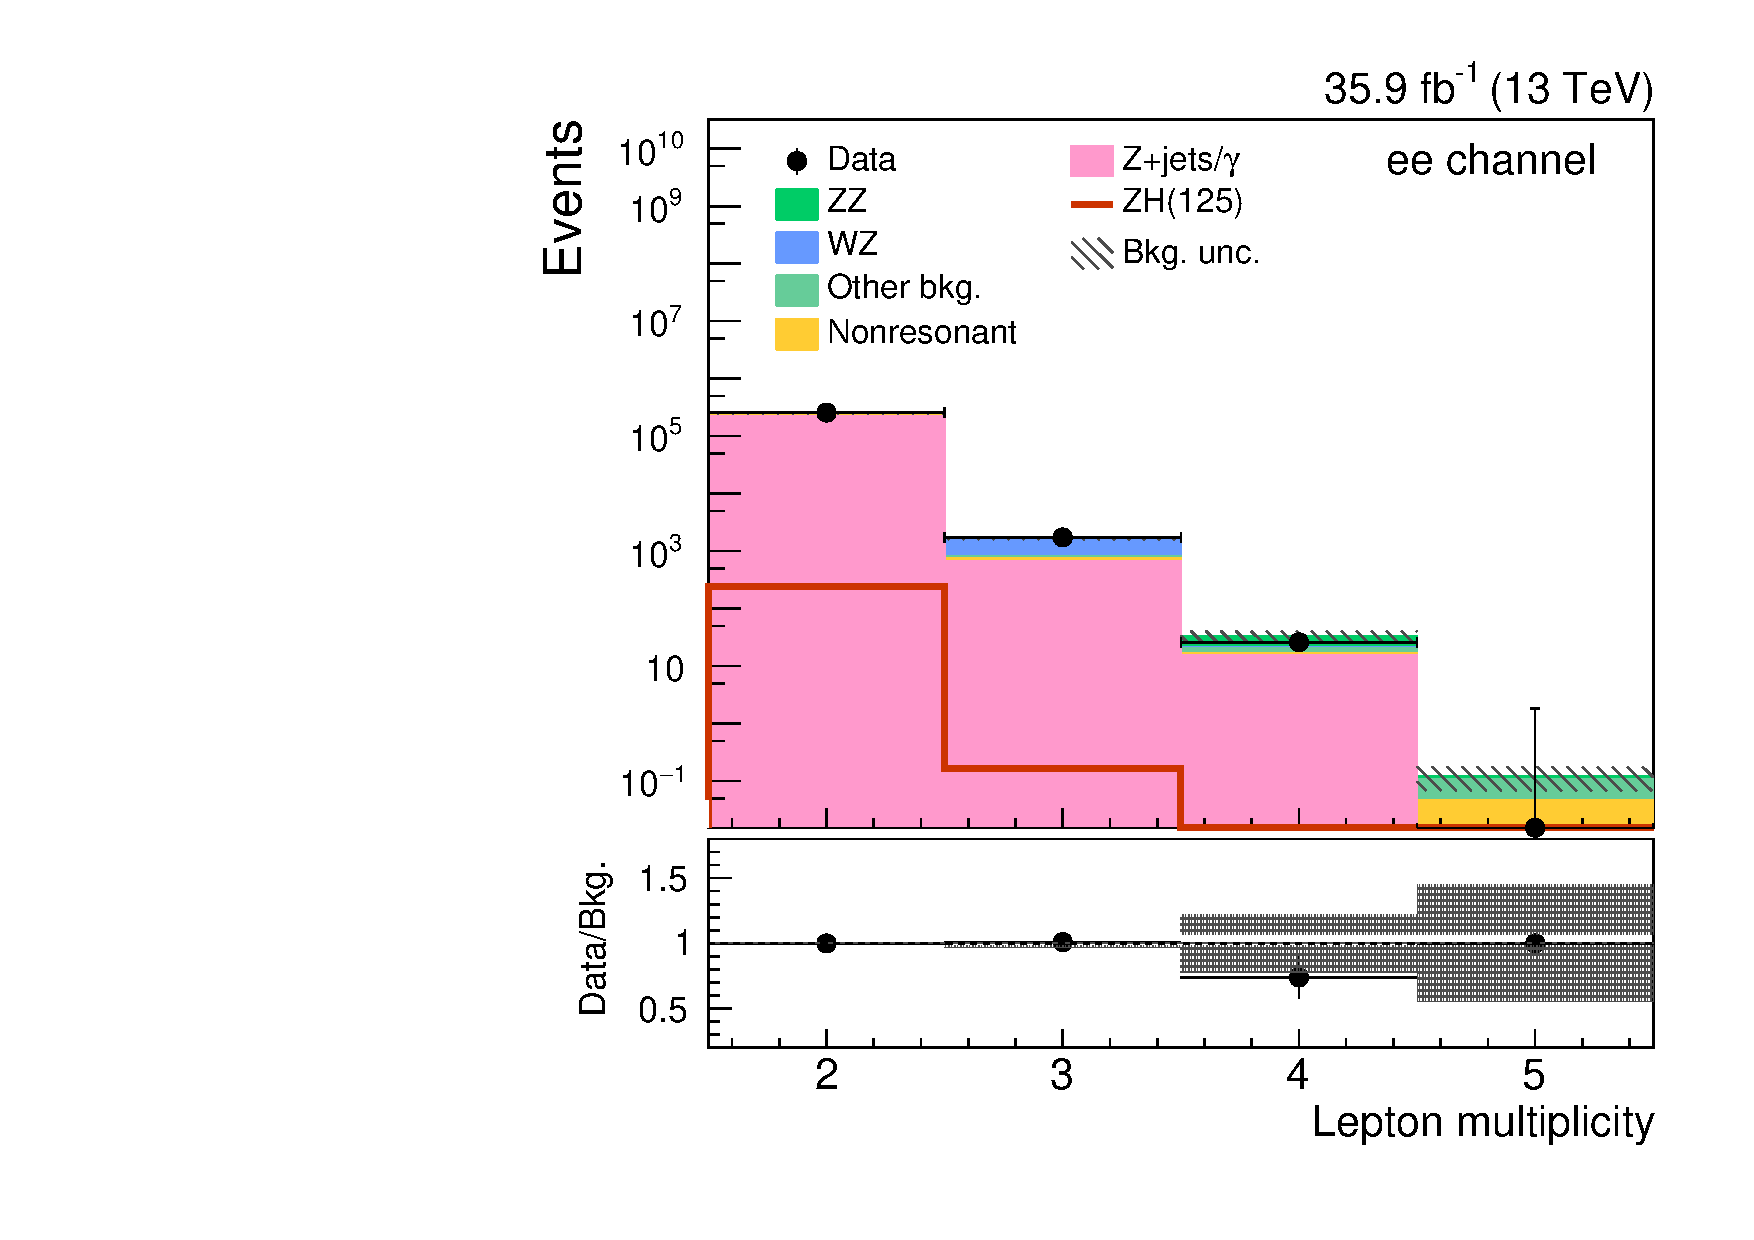
\includegraphics[width=\cmsFigWidth]{figures/zsel_nlep_ee.pdf}
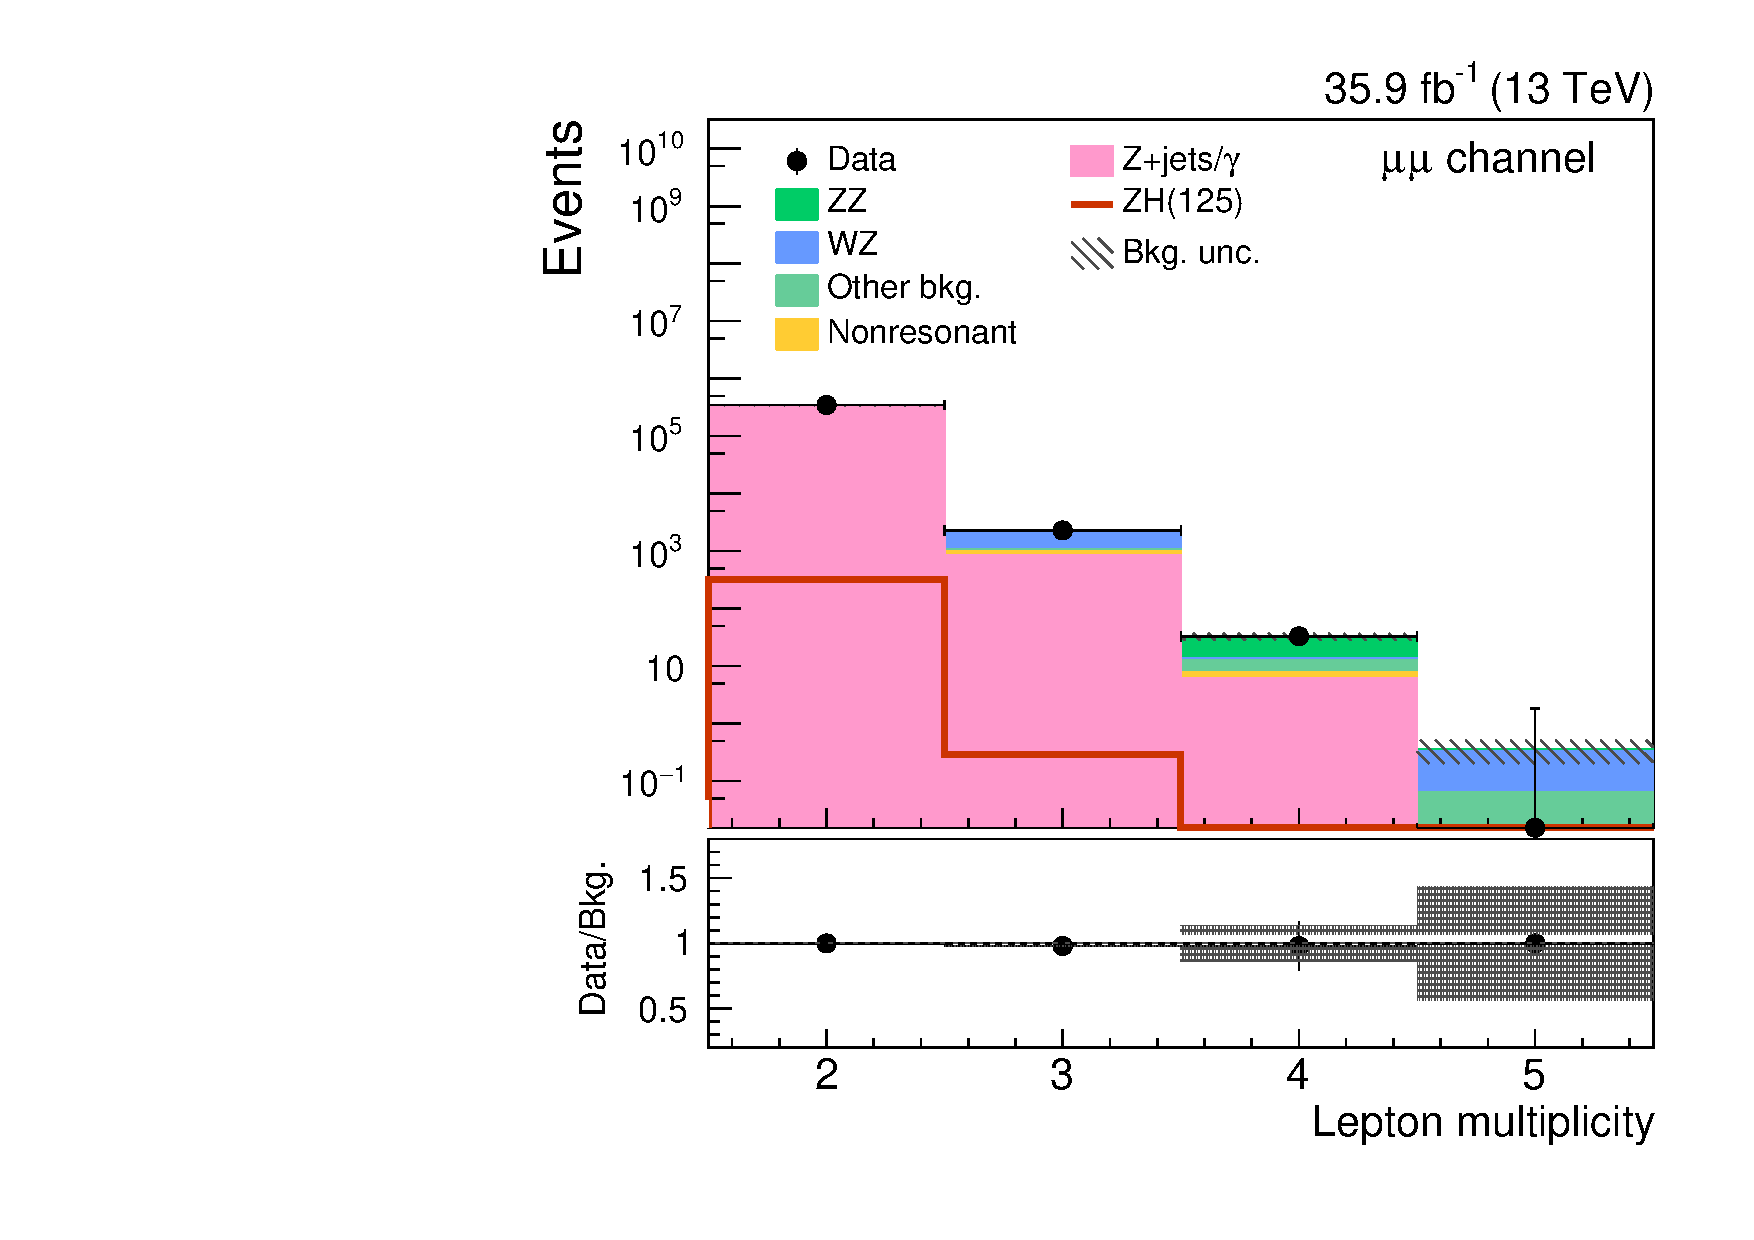
\includegraphics[width=\cmsFigWidth]{figures/zsel_nlep_mm.pdf}
\caption{
  Lepton multiplicity for each flavor channel in $\zll$ events with $\pt^{\ell\ell} > 60~\GeV$ and $\met > 40~\GeV$. 
  The uncertainty band corresponds to the statistical uncertainty only. Left: dielectron channel. Right: dimuon channel.
}
\label{fig:distributions_zsel_nlep}
\end{center}
\end{figure}
\begin{figure}[!hbtp]
\begin{center}
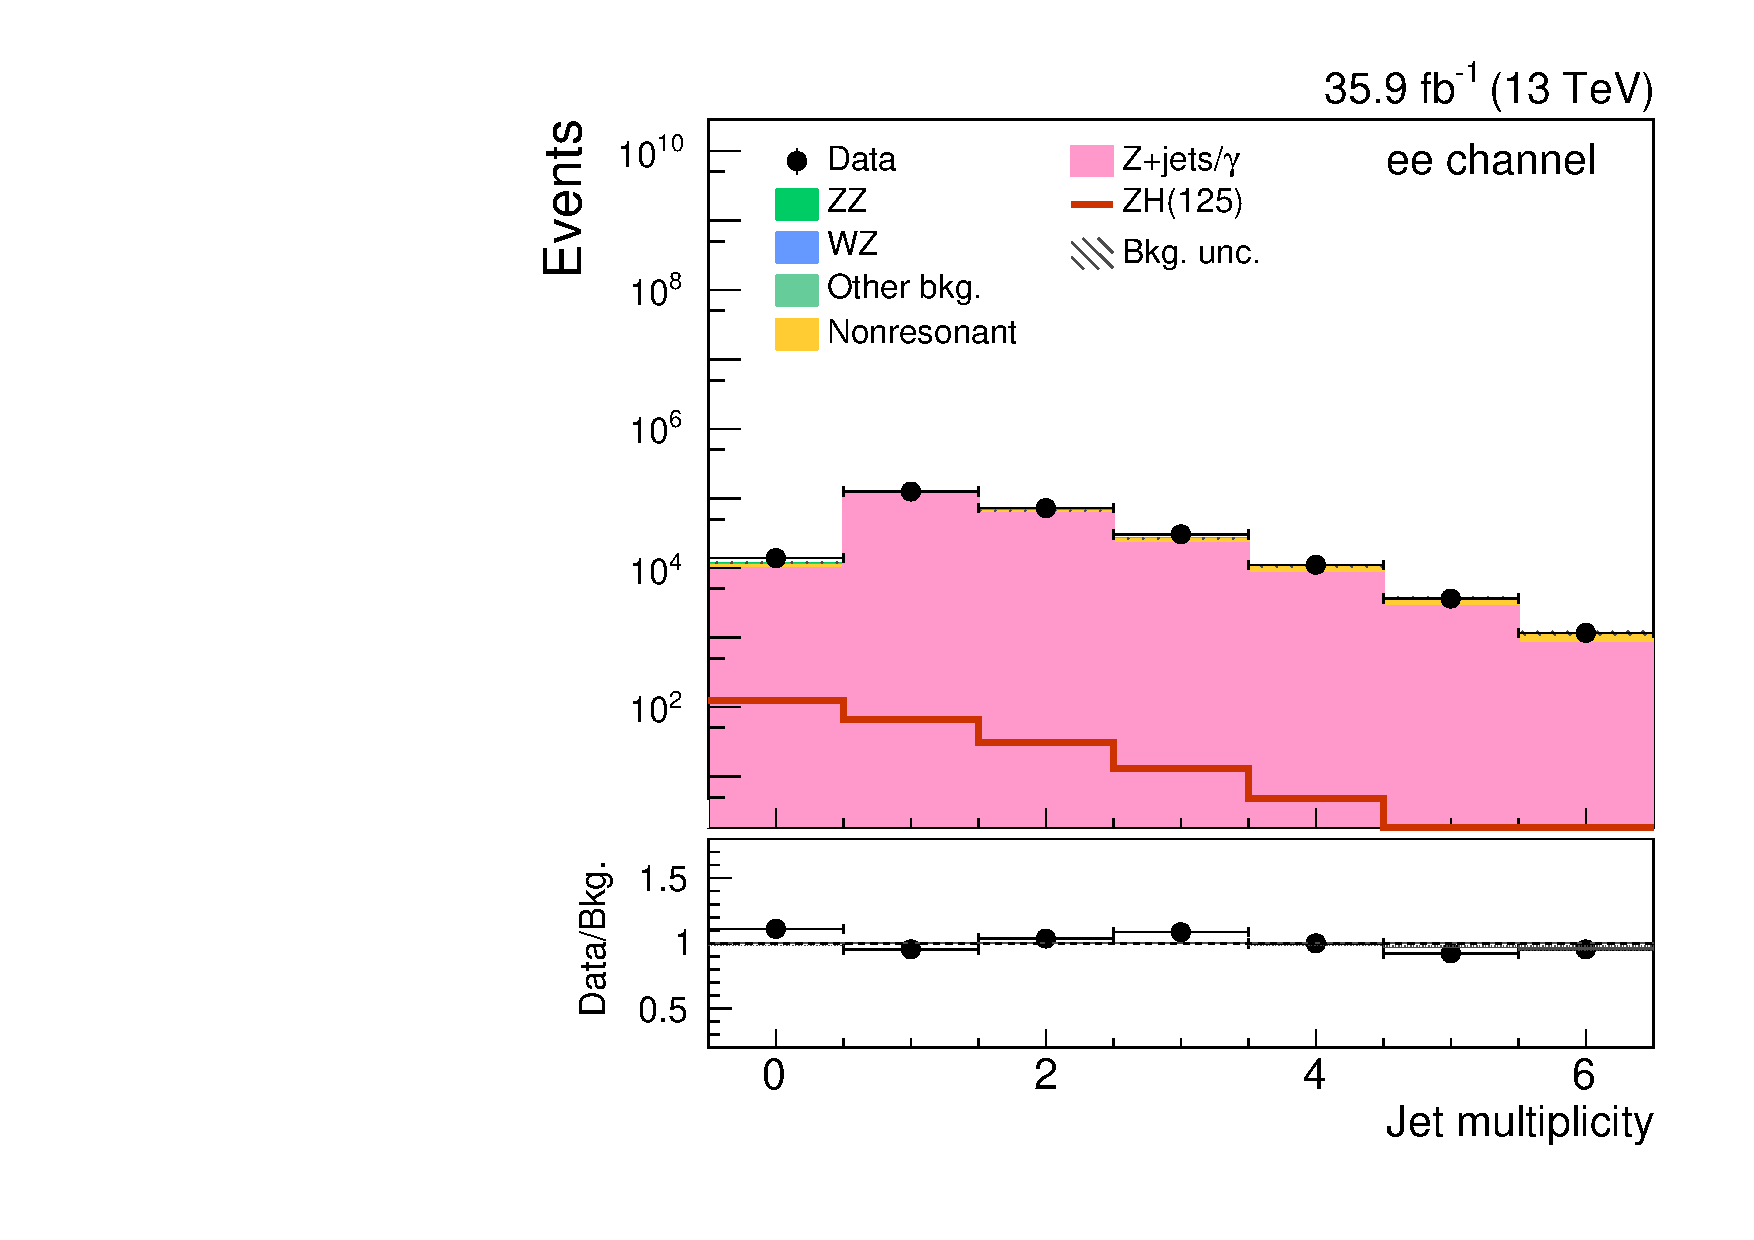
\includegraphics[width=\cmsFigWidth]{figures/zsel_njets_ee.pdf}
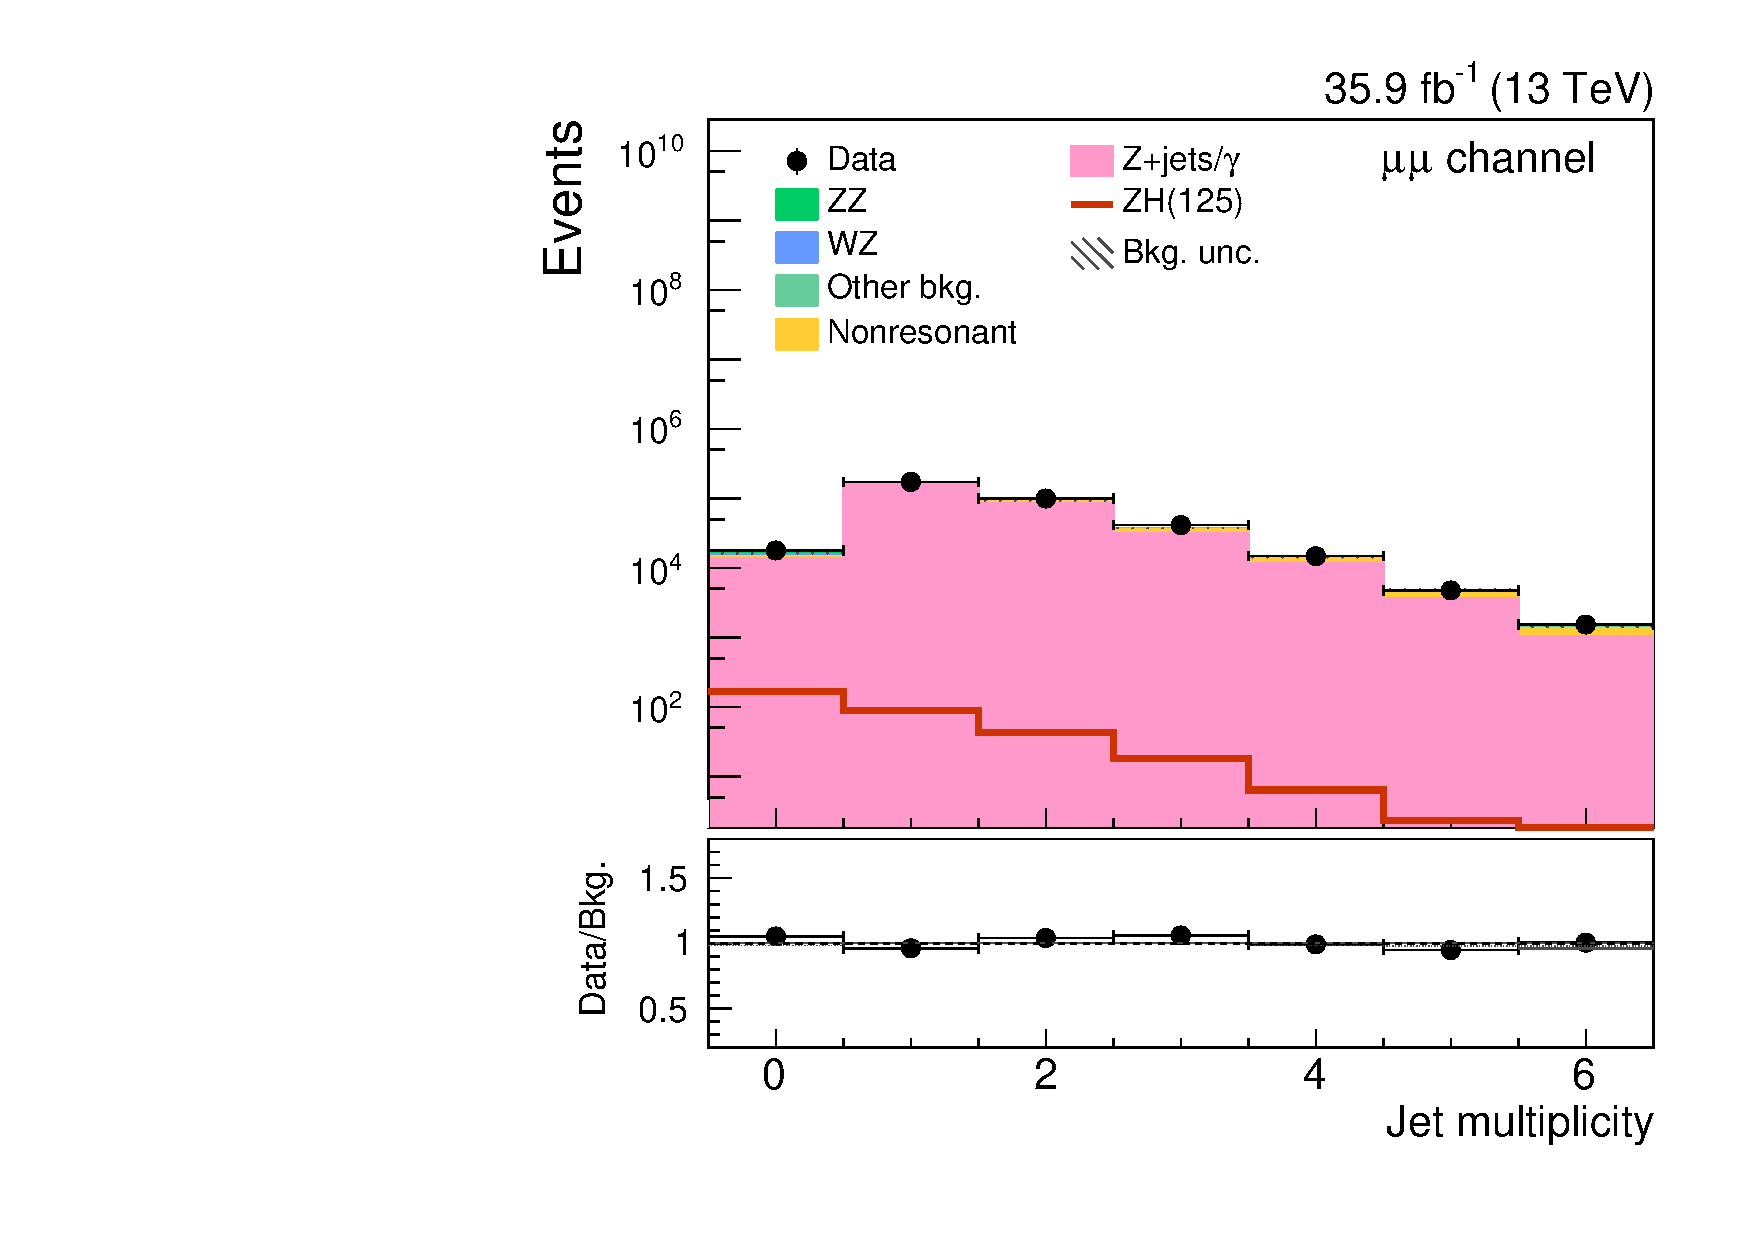
\includegraphics[width=\cmsFigWidth]{figures/zsel_njets_mm.pdf}
\caption{
  Jet multiplicity for each flavor channel in $\zll$ events with $\pt^{\ell\ell} > 60~\GeV$ and $\met > 40~\GeV$. 
  The uncertainty band corresponds to the statistical uncertainty only. Left: dielectron channel. Right: dimuon channel.
}
\label{fig:distributions_zsel_njets}
\end{center}
\end{figure}
\begin{figure}[!hbtp]
\begin{center}
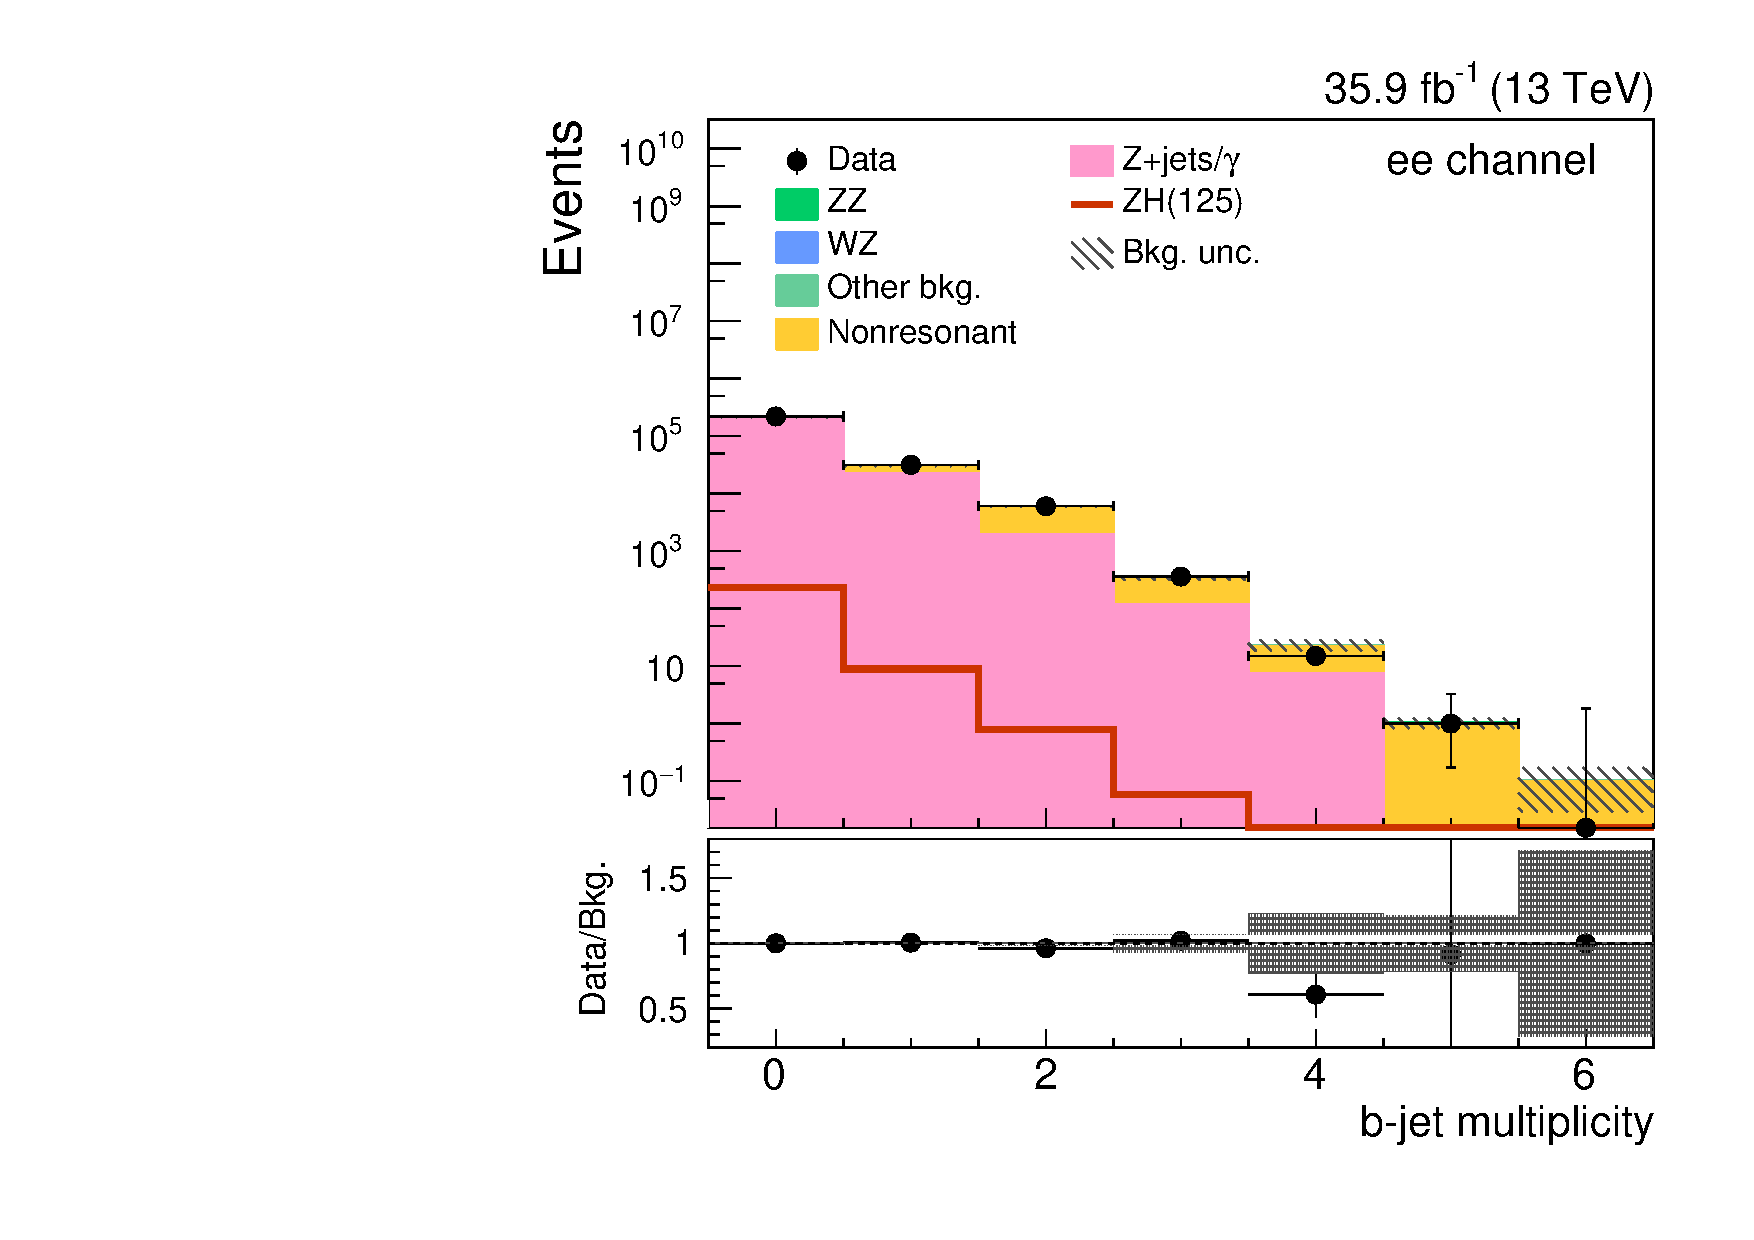
\includegraphics[width=\cmsFigWidth]{figures/zsel_bjets_ee.pdf}
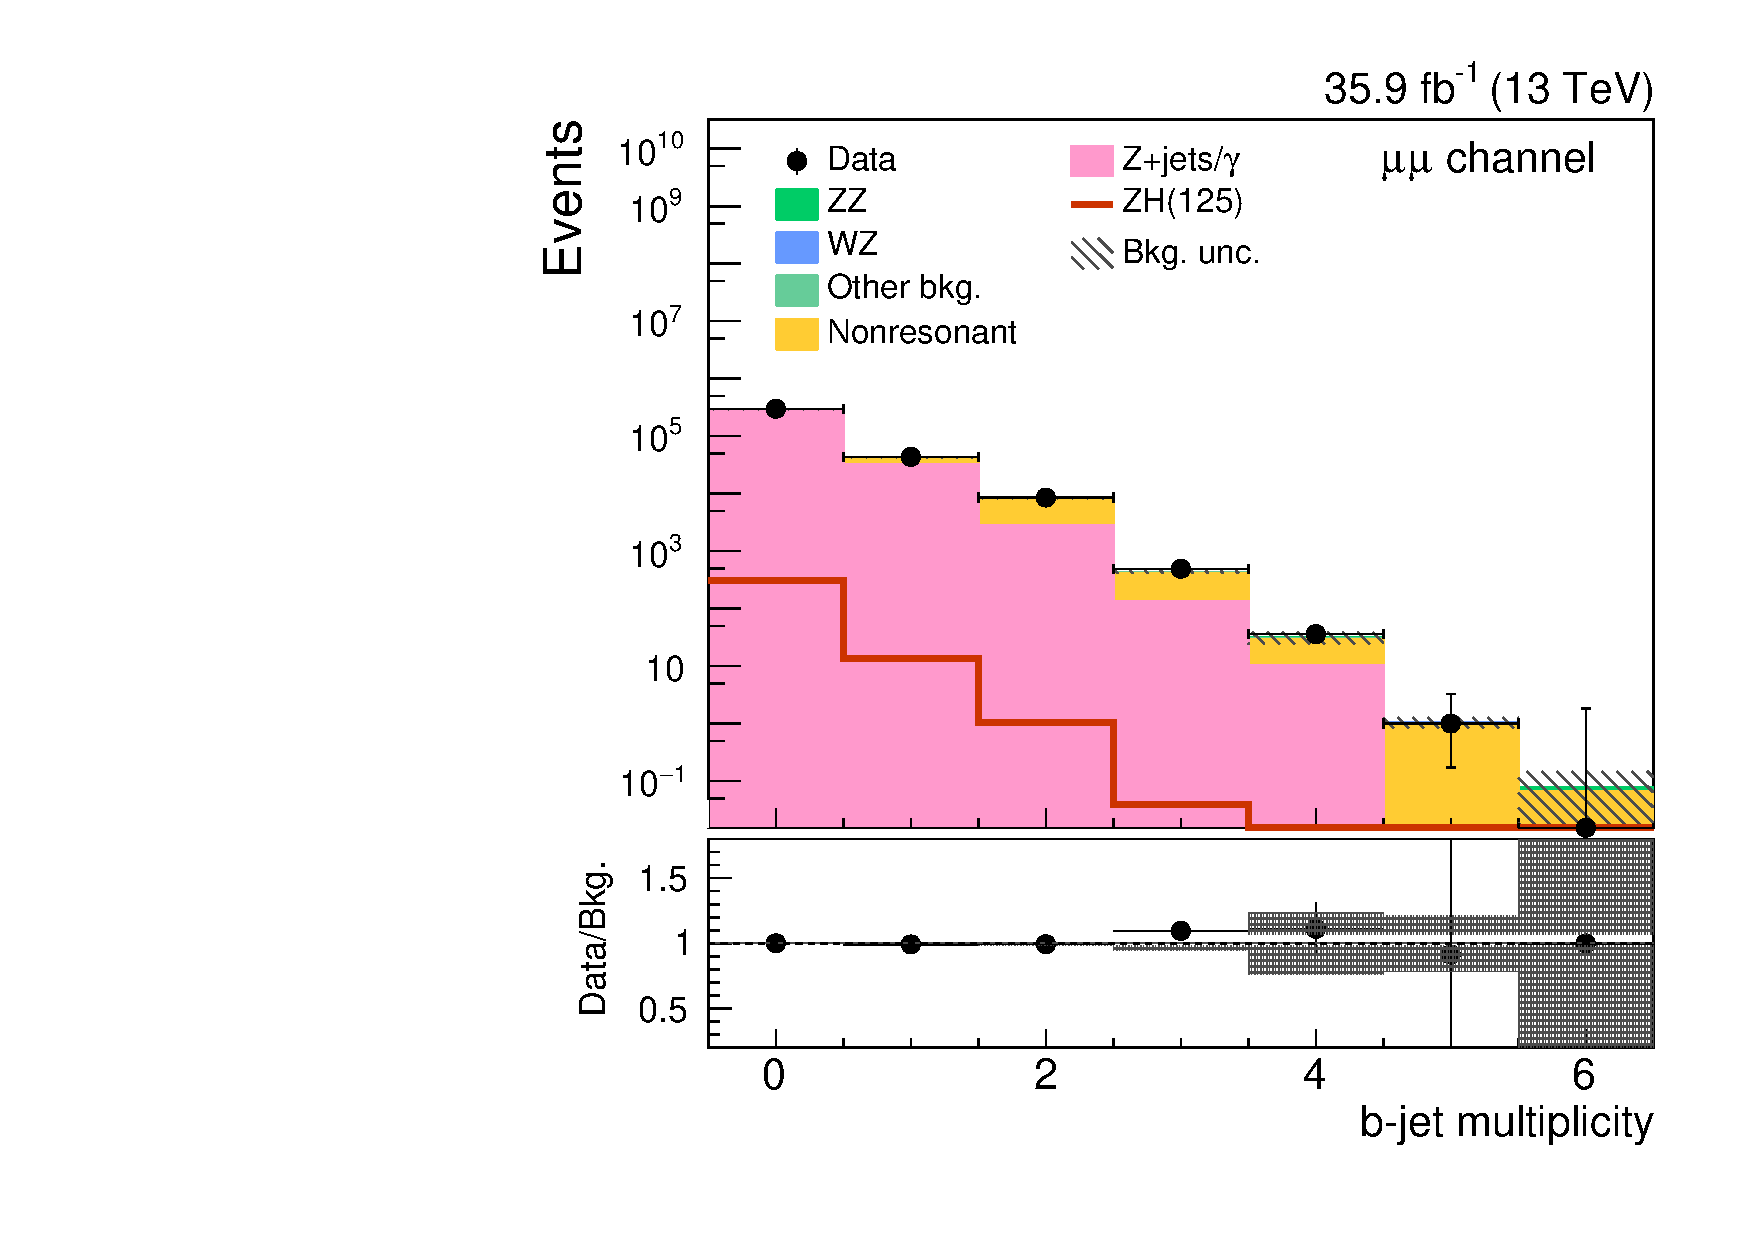
\includegraphics[width=\cmsFigWidth]{figures/zsel_bjets_mm.pdf}
\caption{
  Number of jets passing the requirements for b-tagging for each flavor channel in $\zll$ events with $\pt^{\ell\ell} > 60~\GeV$ and $\met > 40~\GeV$. 
  The uncertainty band corresponds to the statistical uncertainty only. Left: dielectron channel. Right: dimuon channel.
}
\label{fig:distributions_zsel_bjets}
\end{center}
\end{figure}
\begin{figure}[!hbtp]
\begin{center}
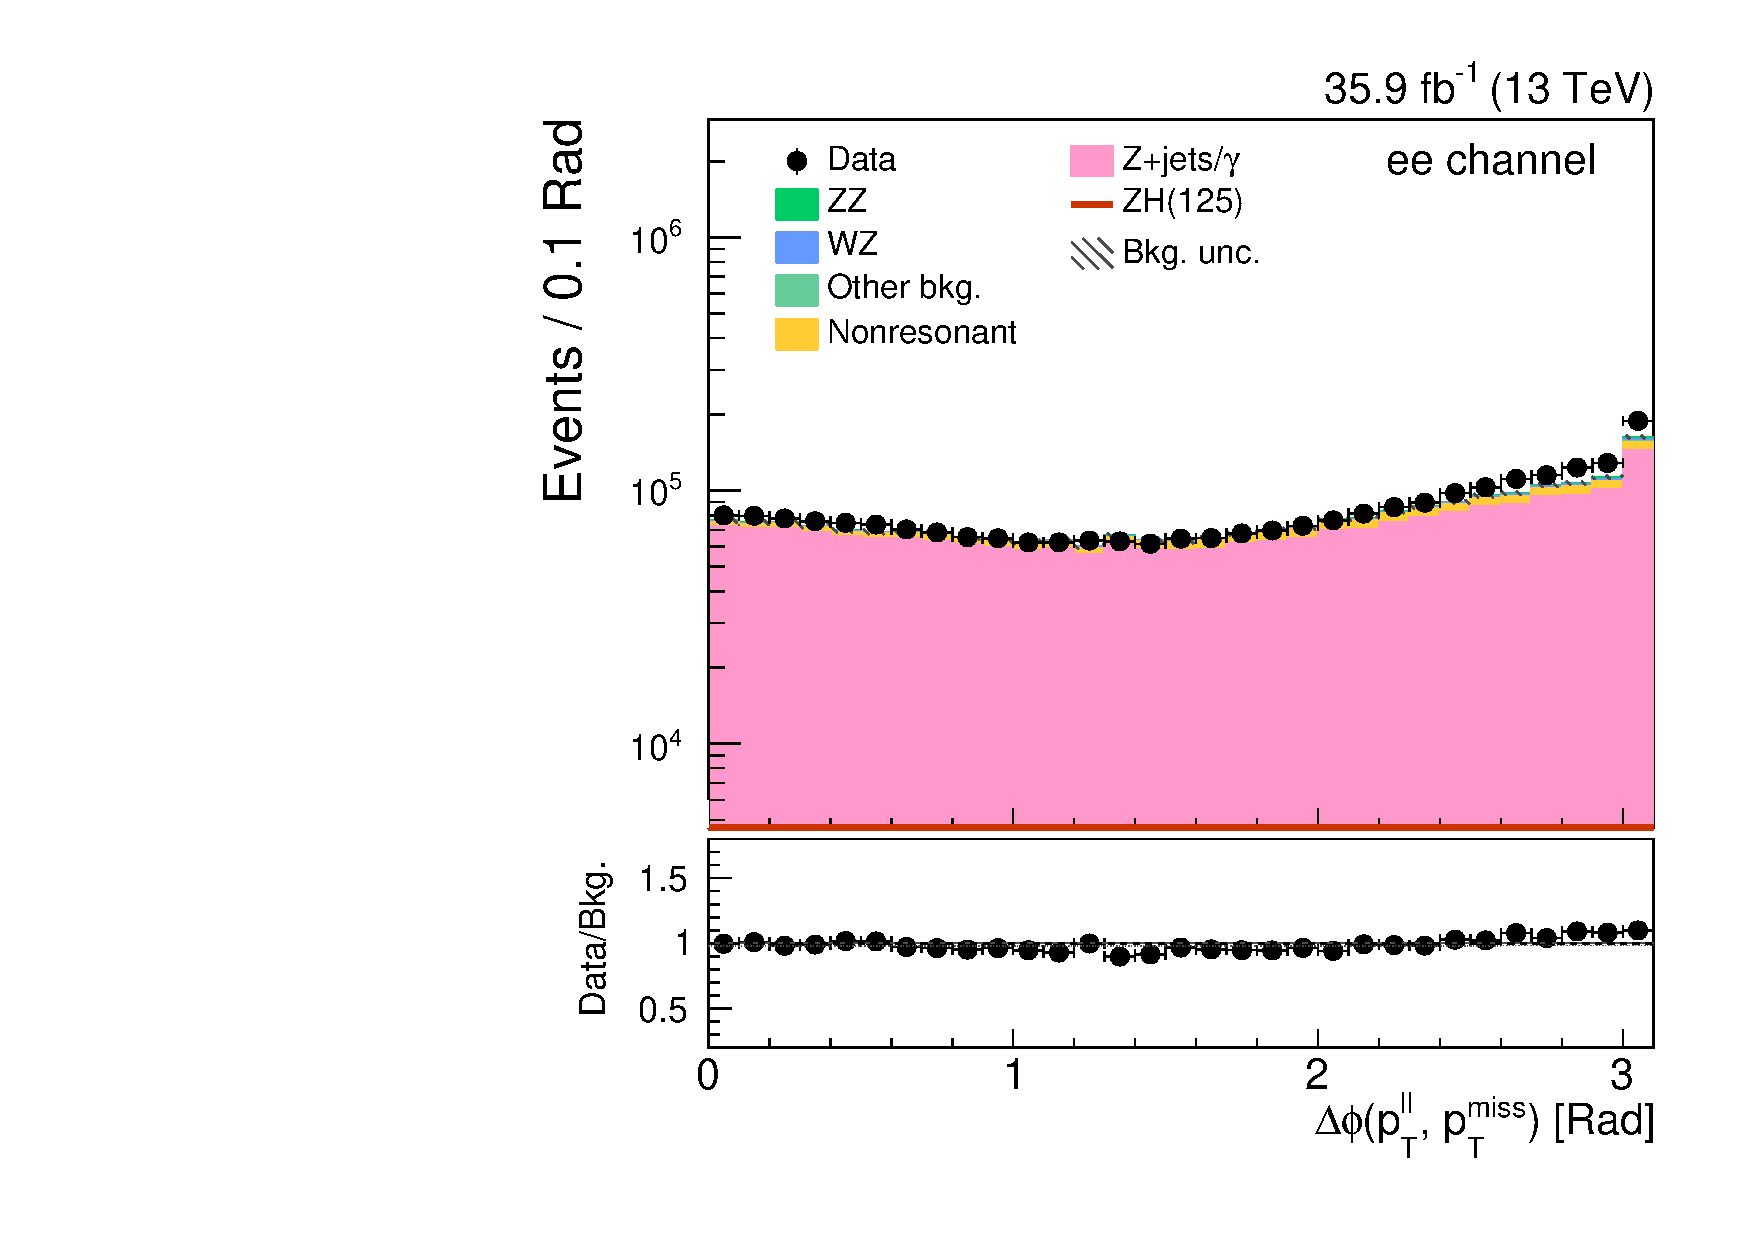
\includegraphics[width=\cmsFigWidth]{figures/zsel_dphiZMET_ee.pdf}
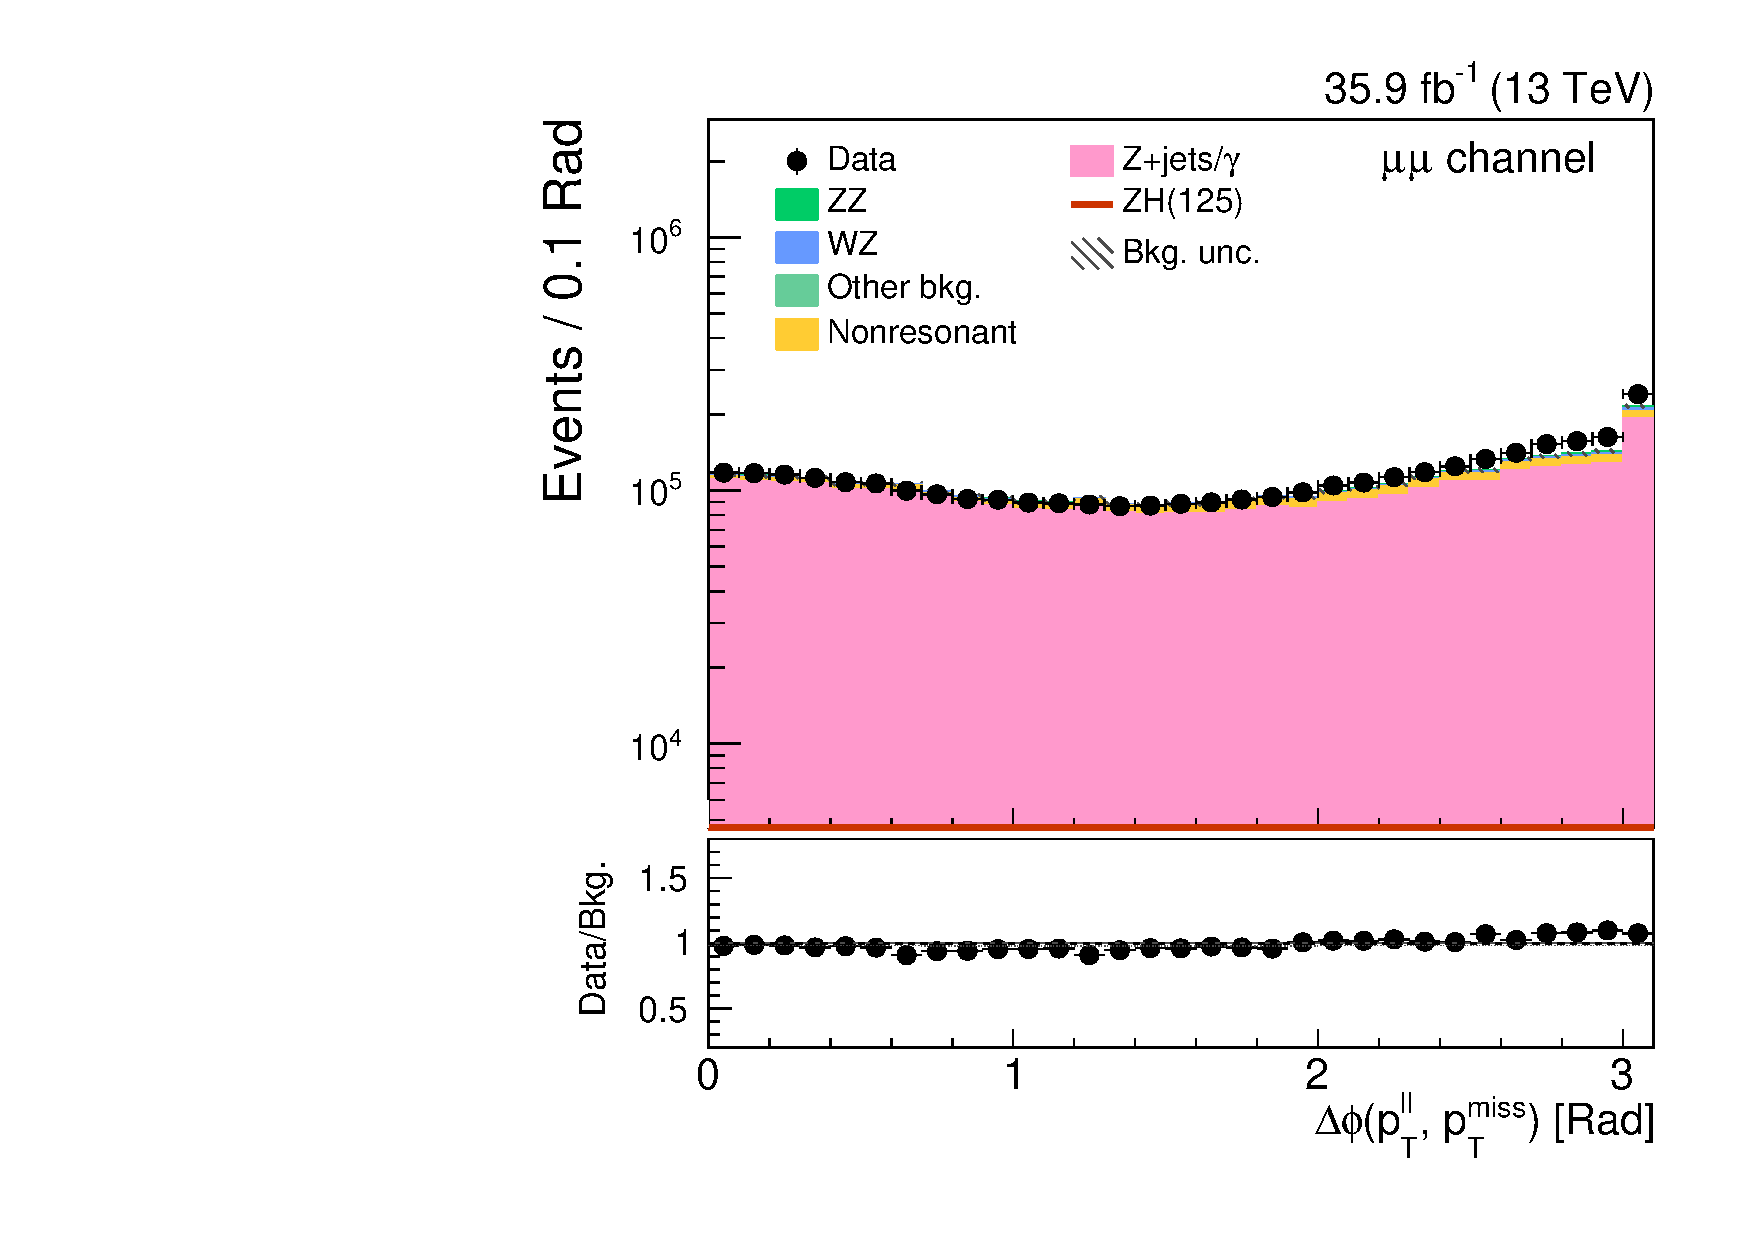
\includegraphics[width=\cmsFigWidth]{figures/zsel_dphiZMET_mm.pdf}
\caption{
  Azimuthal separation between the dilepton system and the missing transverse energy for each flavor channel in $\zll$ events with $\pt^{\ell\ell} > 60~\GeV$ and $\met > 40~\GeV$. 
  The uncertainty band corresponds to the statistical uncertainty only. Left: dielectron channel. Right: dimuon channel.
}
\label{fig:distributions_zsel_dphiZMET}
\end{center}
\end{figure}

\begin{figure}[!hbtp]
\begin{center}
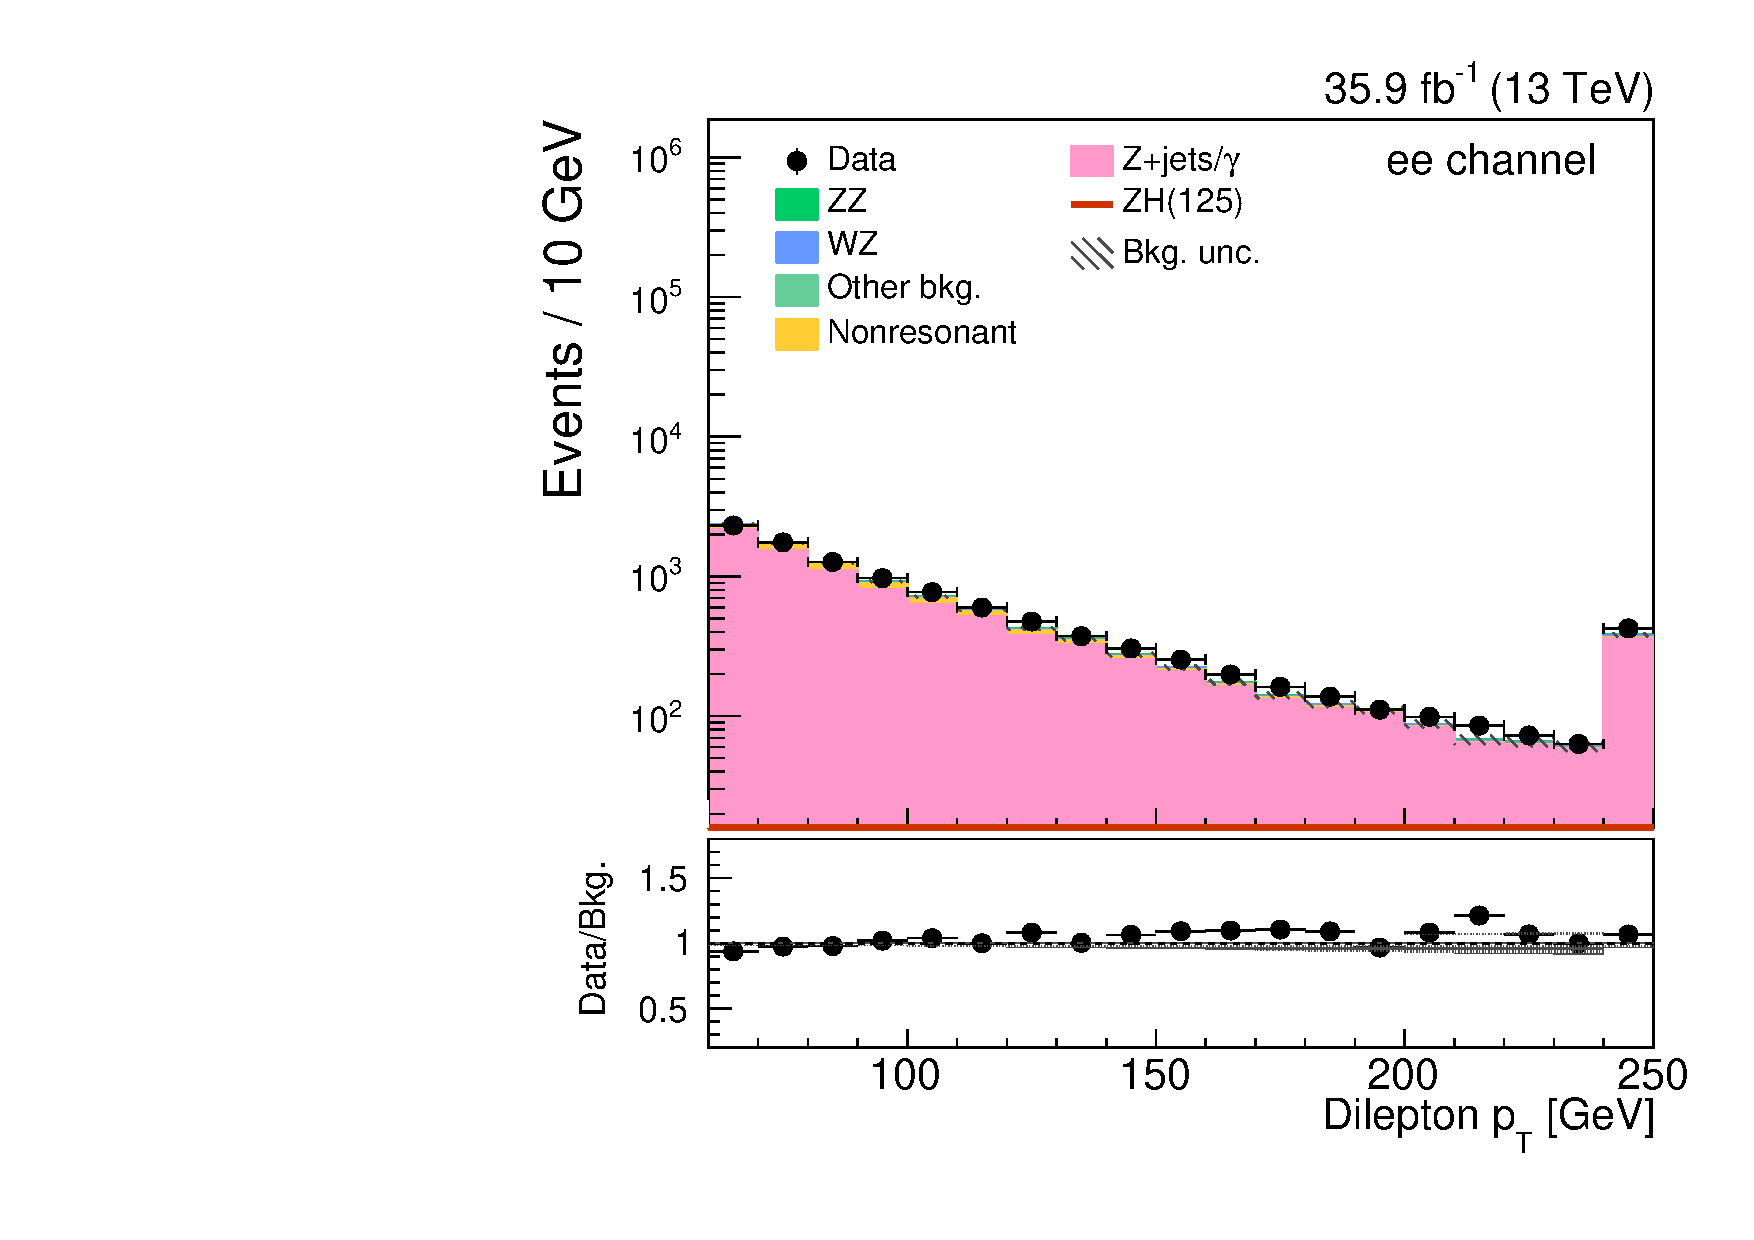
\includegraphics[width=\cmsFigWidth]{figures/presel_ptll_ee.pdf}
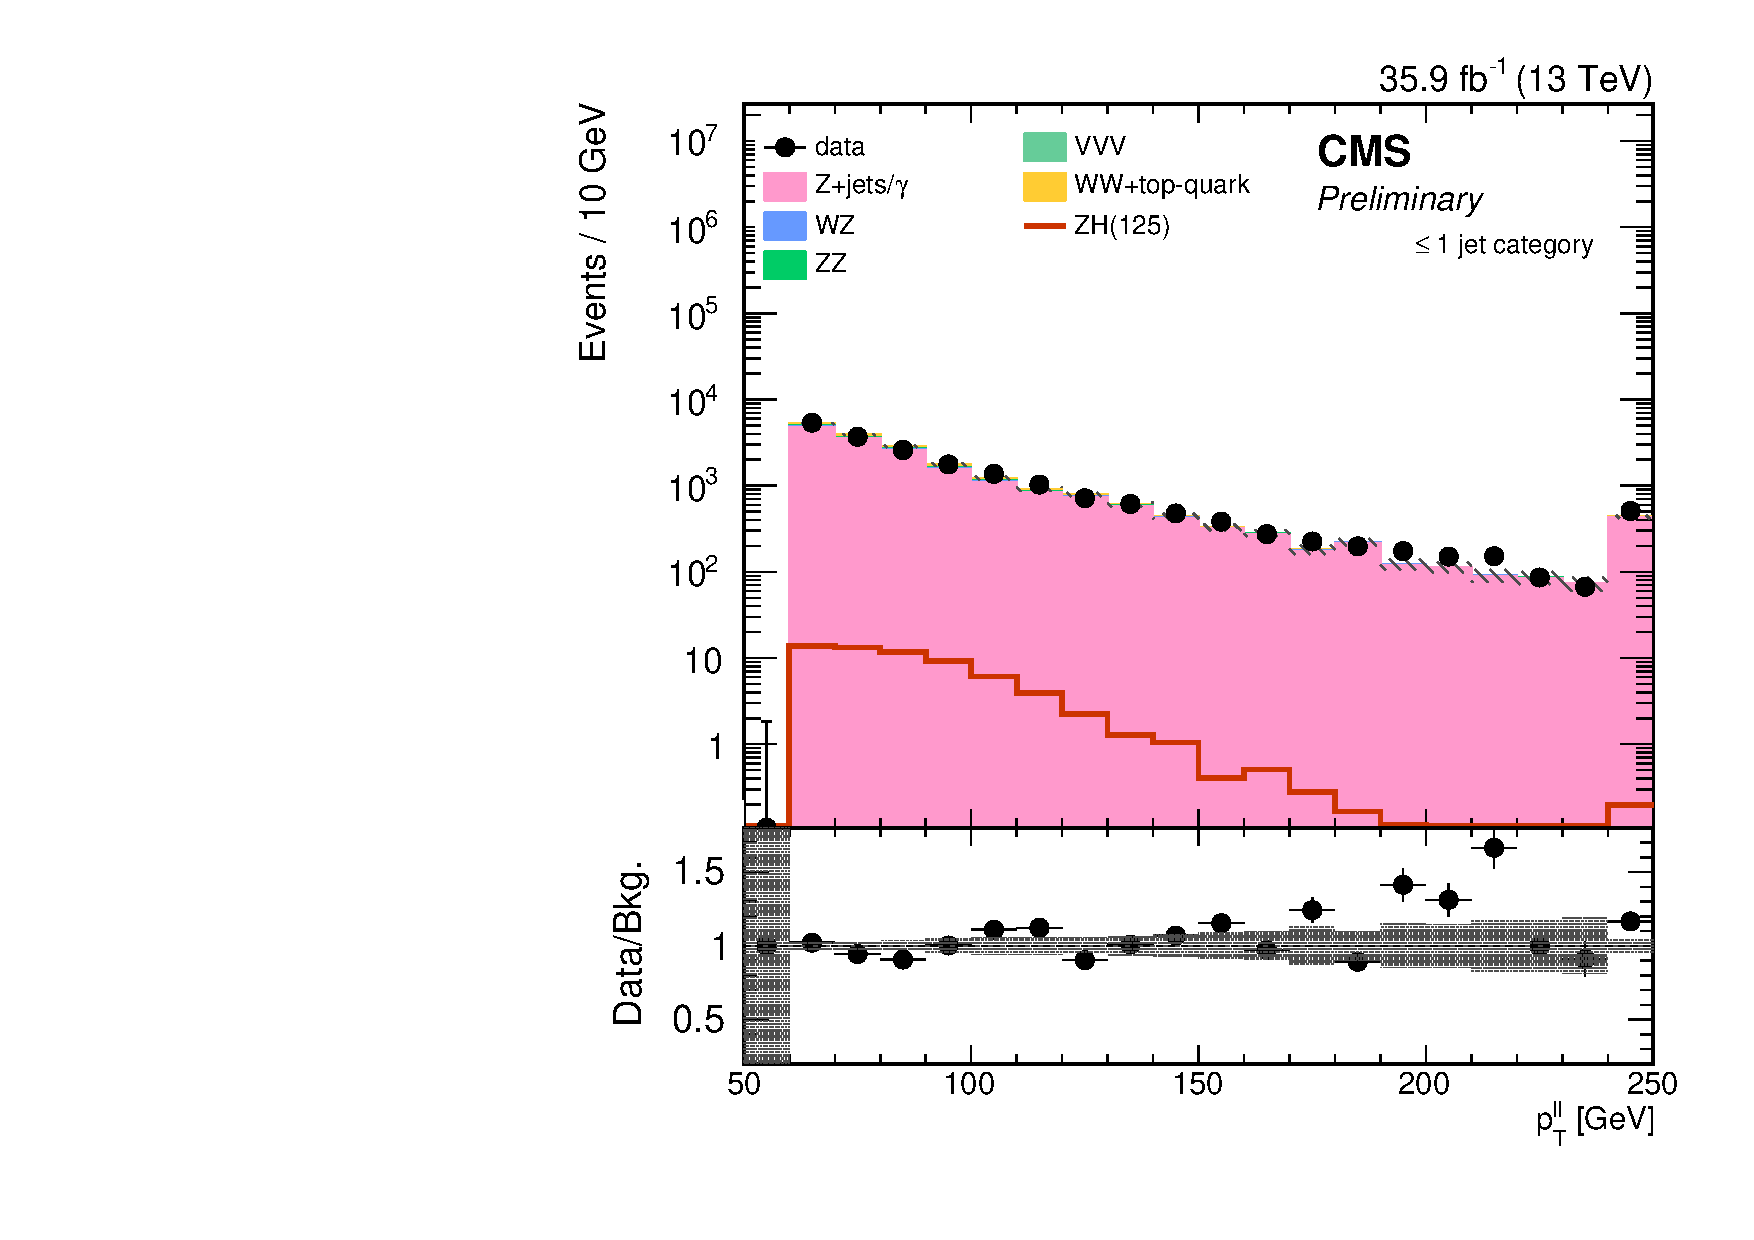
\includegraphics[width=\cmsFigWidth]{figures/presel_ptll_mm.pdf}
\caption{
  Distributions of the $\pt^{\ell\ell}$ for each flavor channel in $\zll$ events with $\pt^{\ell\ell} > 60~\GeV$ and $\met > 40~\GeV$.
  The uncertainty band corresponds to the statistical uncertainty only. Left: dielectron channel. Right: dimuon channel.
}
\label{fig:distributions_presel_ptll}
\end{center}
\end{figure}
\begin{figure}[!hbtp]
\begin{center}
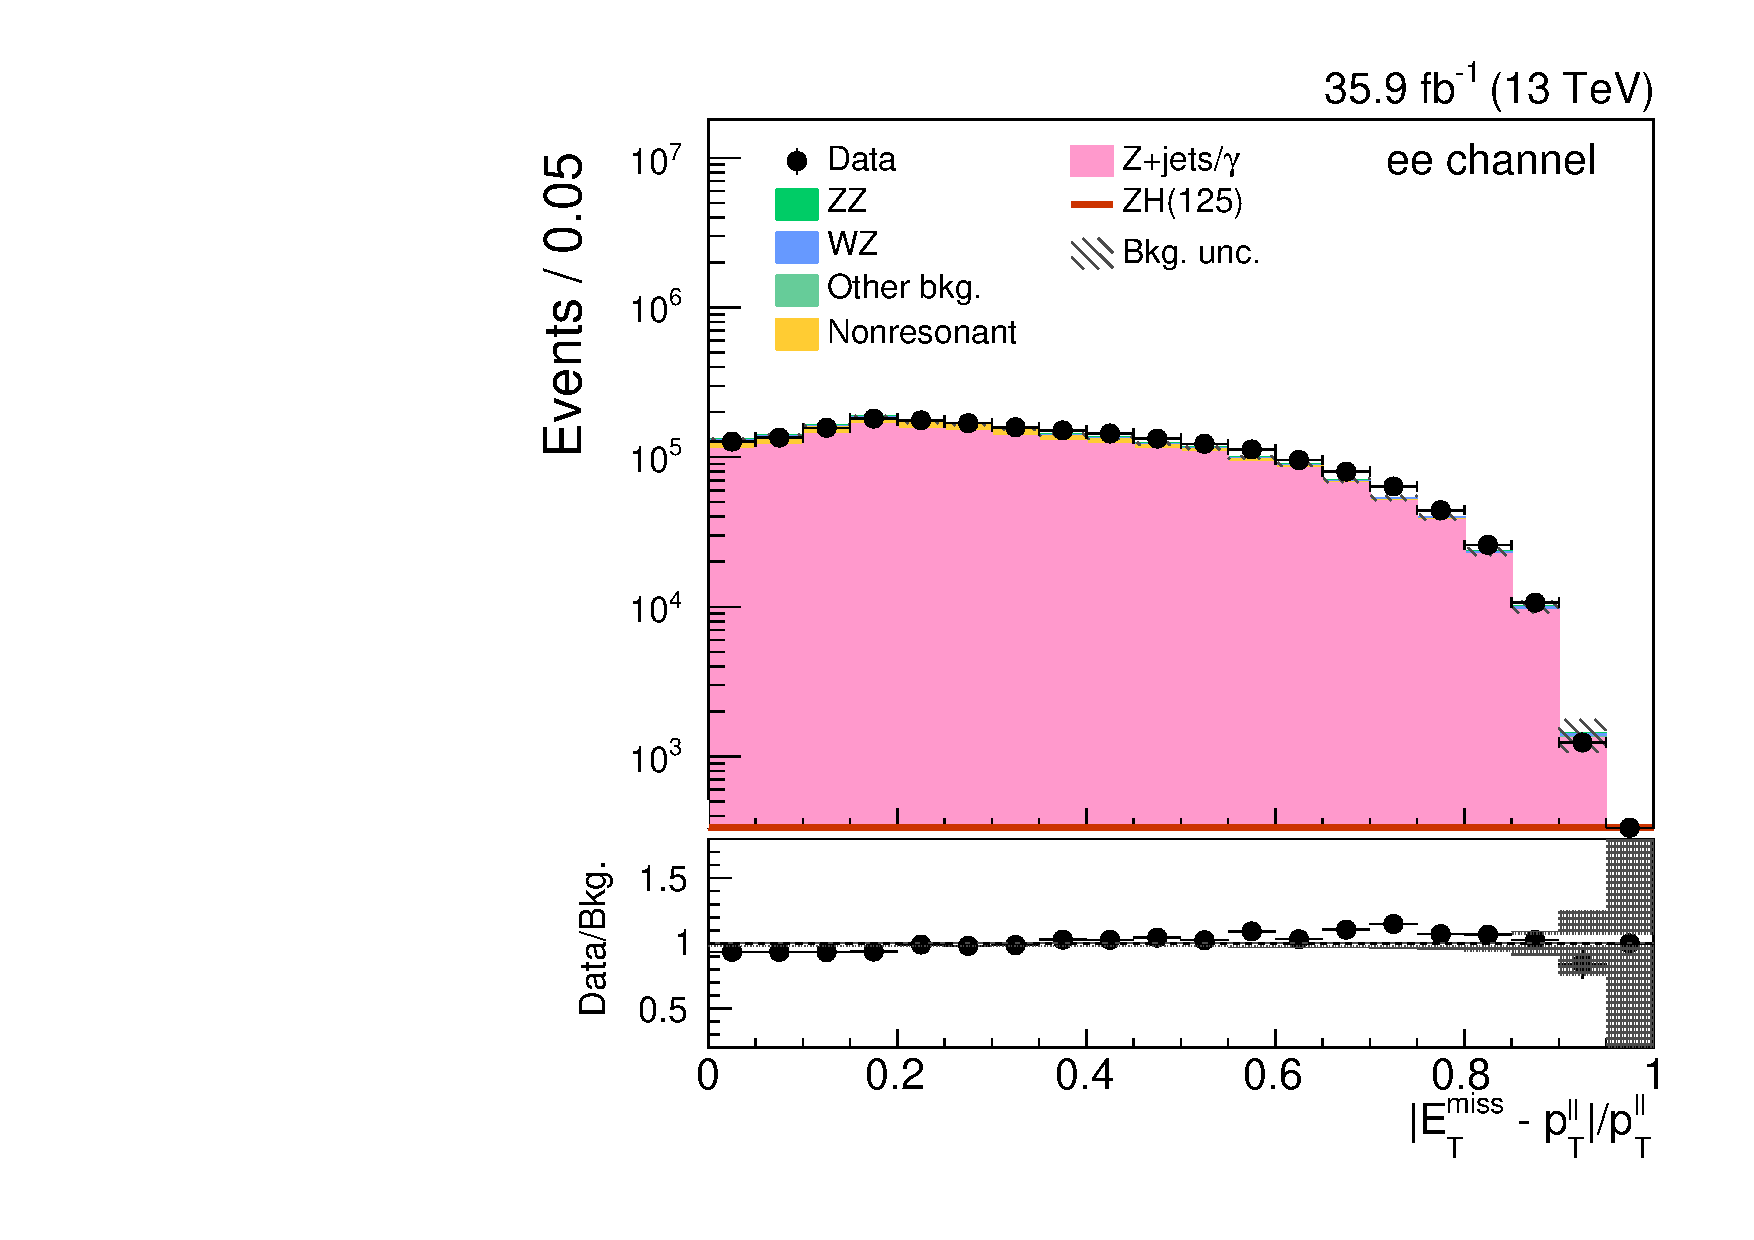
\includegraphics[width=\cmsFigWidth]{figures/presel_balance_ee.pdf}
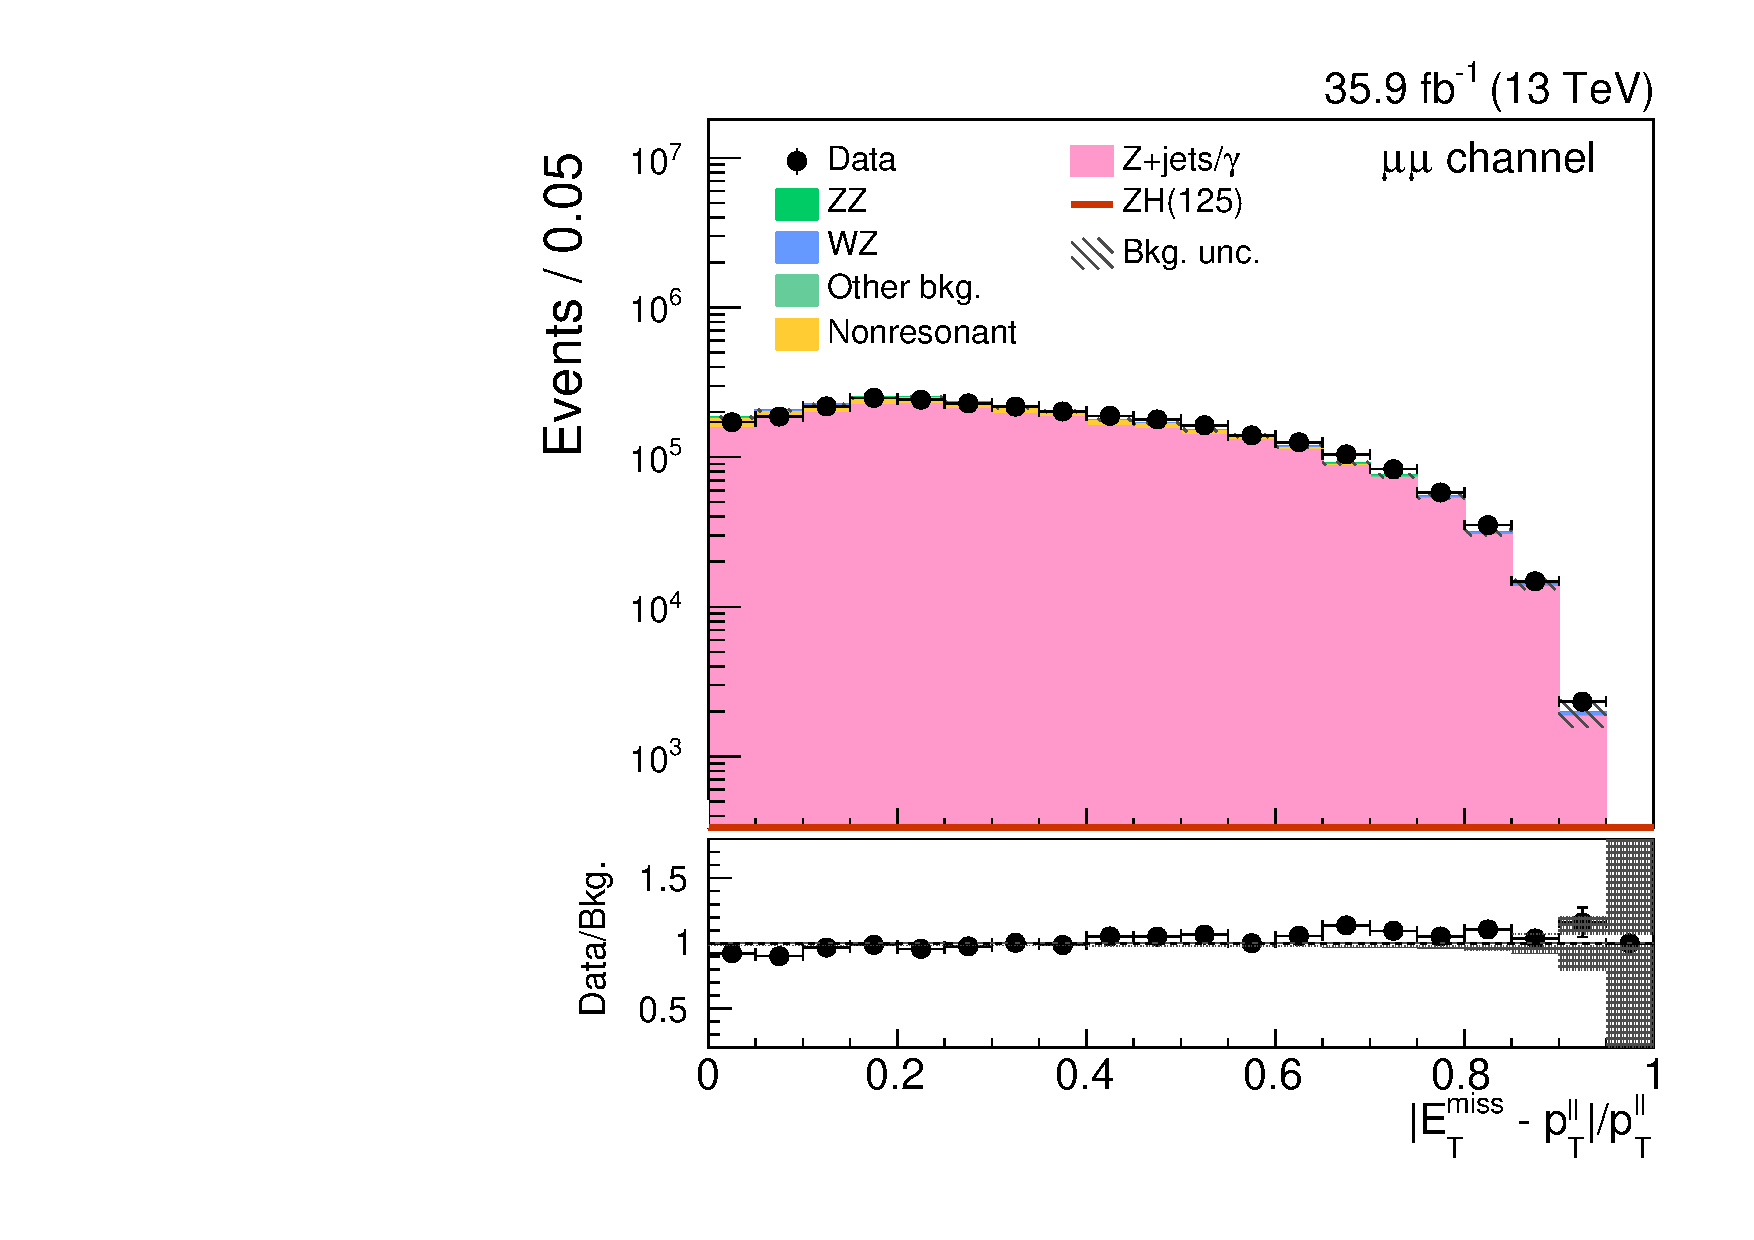
\includegraphics[width=\cmsFigWidth]{figures/presel_balance_mm.pdf}
\caption{
  Distributions of the balance variable $|\met-\pt^{\ell\ell}|/\pt^{\ell\ell}$ for each flavor channel in $\zll$ events with $\pt^{\ell\ell} > 60~\GeV$ and $\met > 40~\GeV$. 
  The uncertainty band corresponds to the statistical uncertainty only. Left: dielectron channel. Right: dimuon channel.
}
\label{fig:distributions_presel_balance}
\end{center}
\end{figure}
\clearpage

\begin{figure}[!hbtp]
\begin{center}
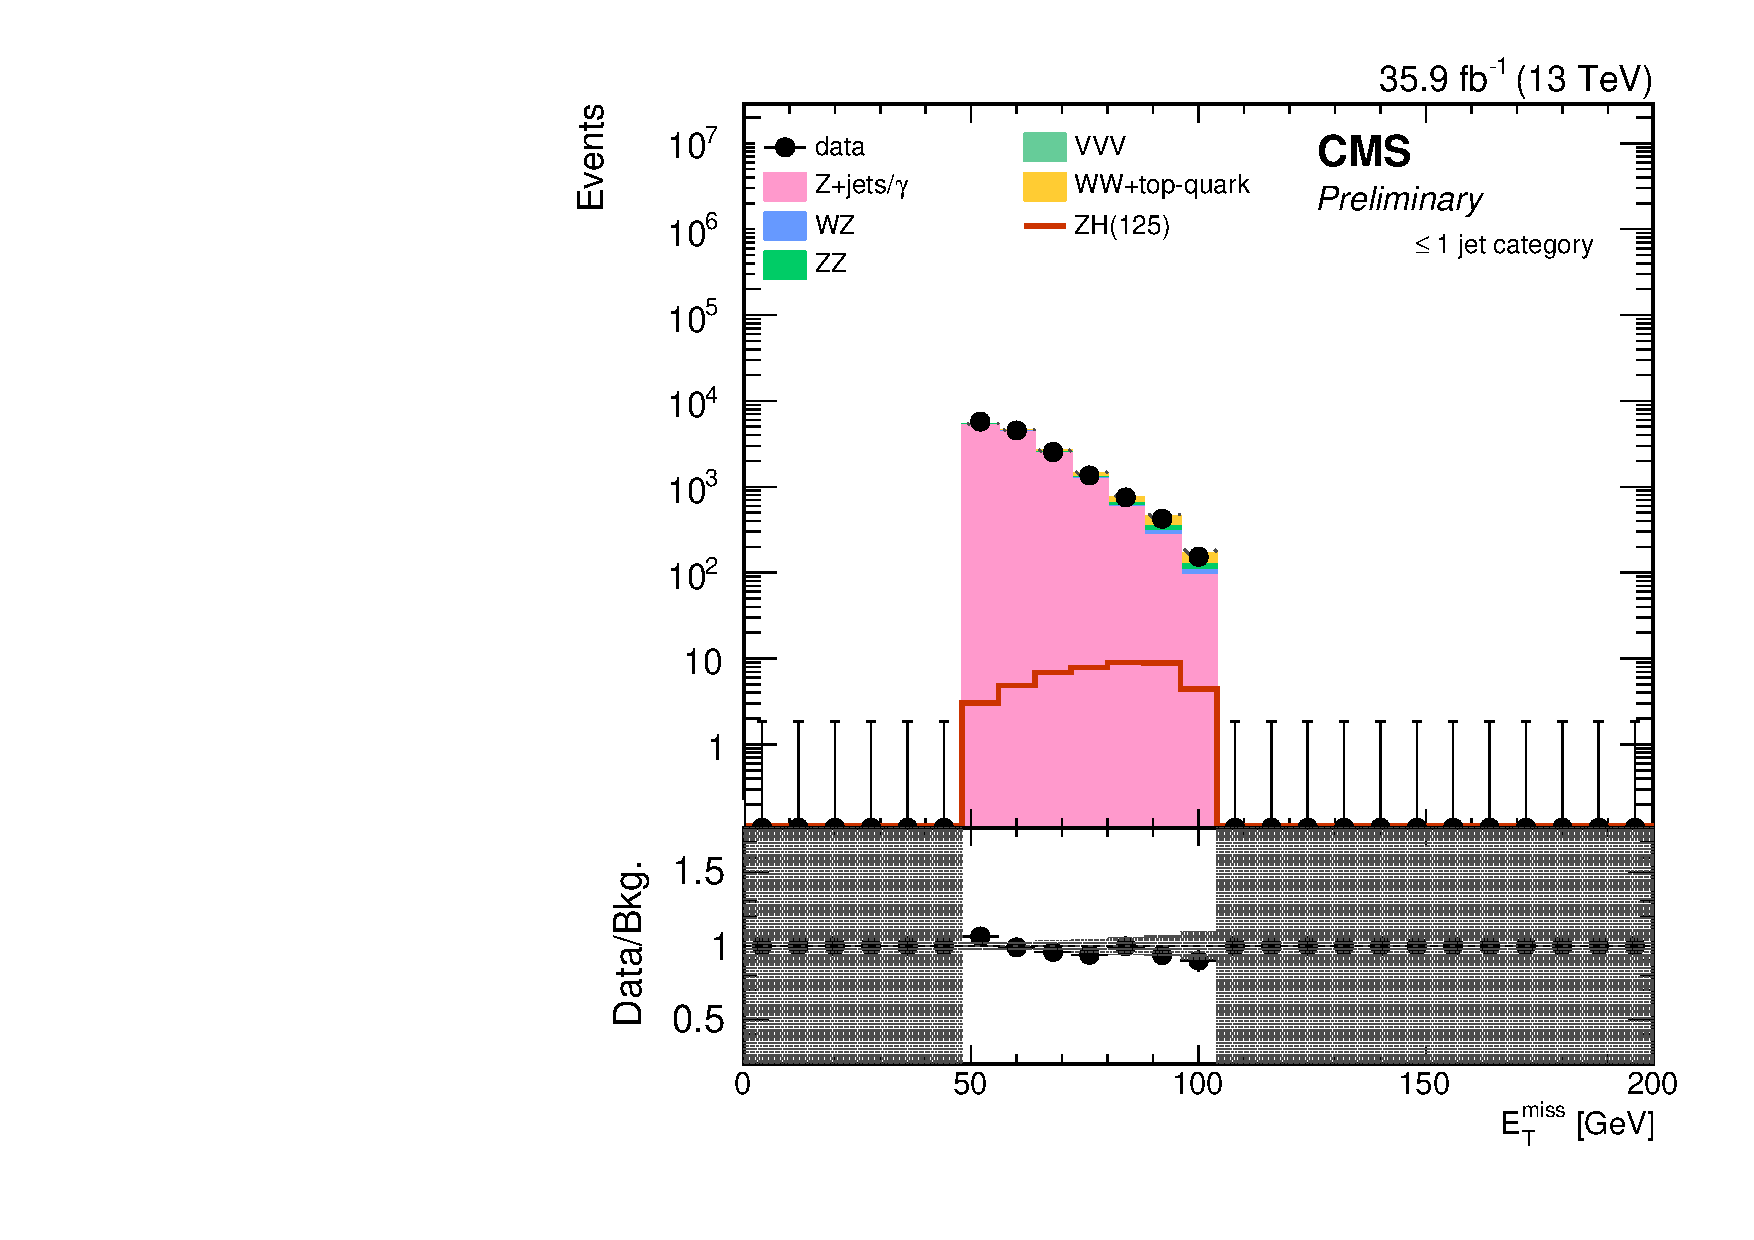
\includegraphics[width=\cmsFigWidth]{figures/presel_met_ee.pdf}
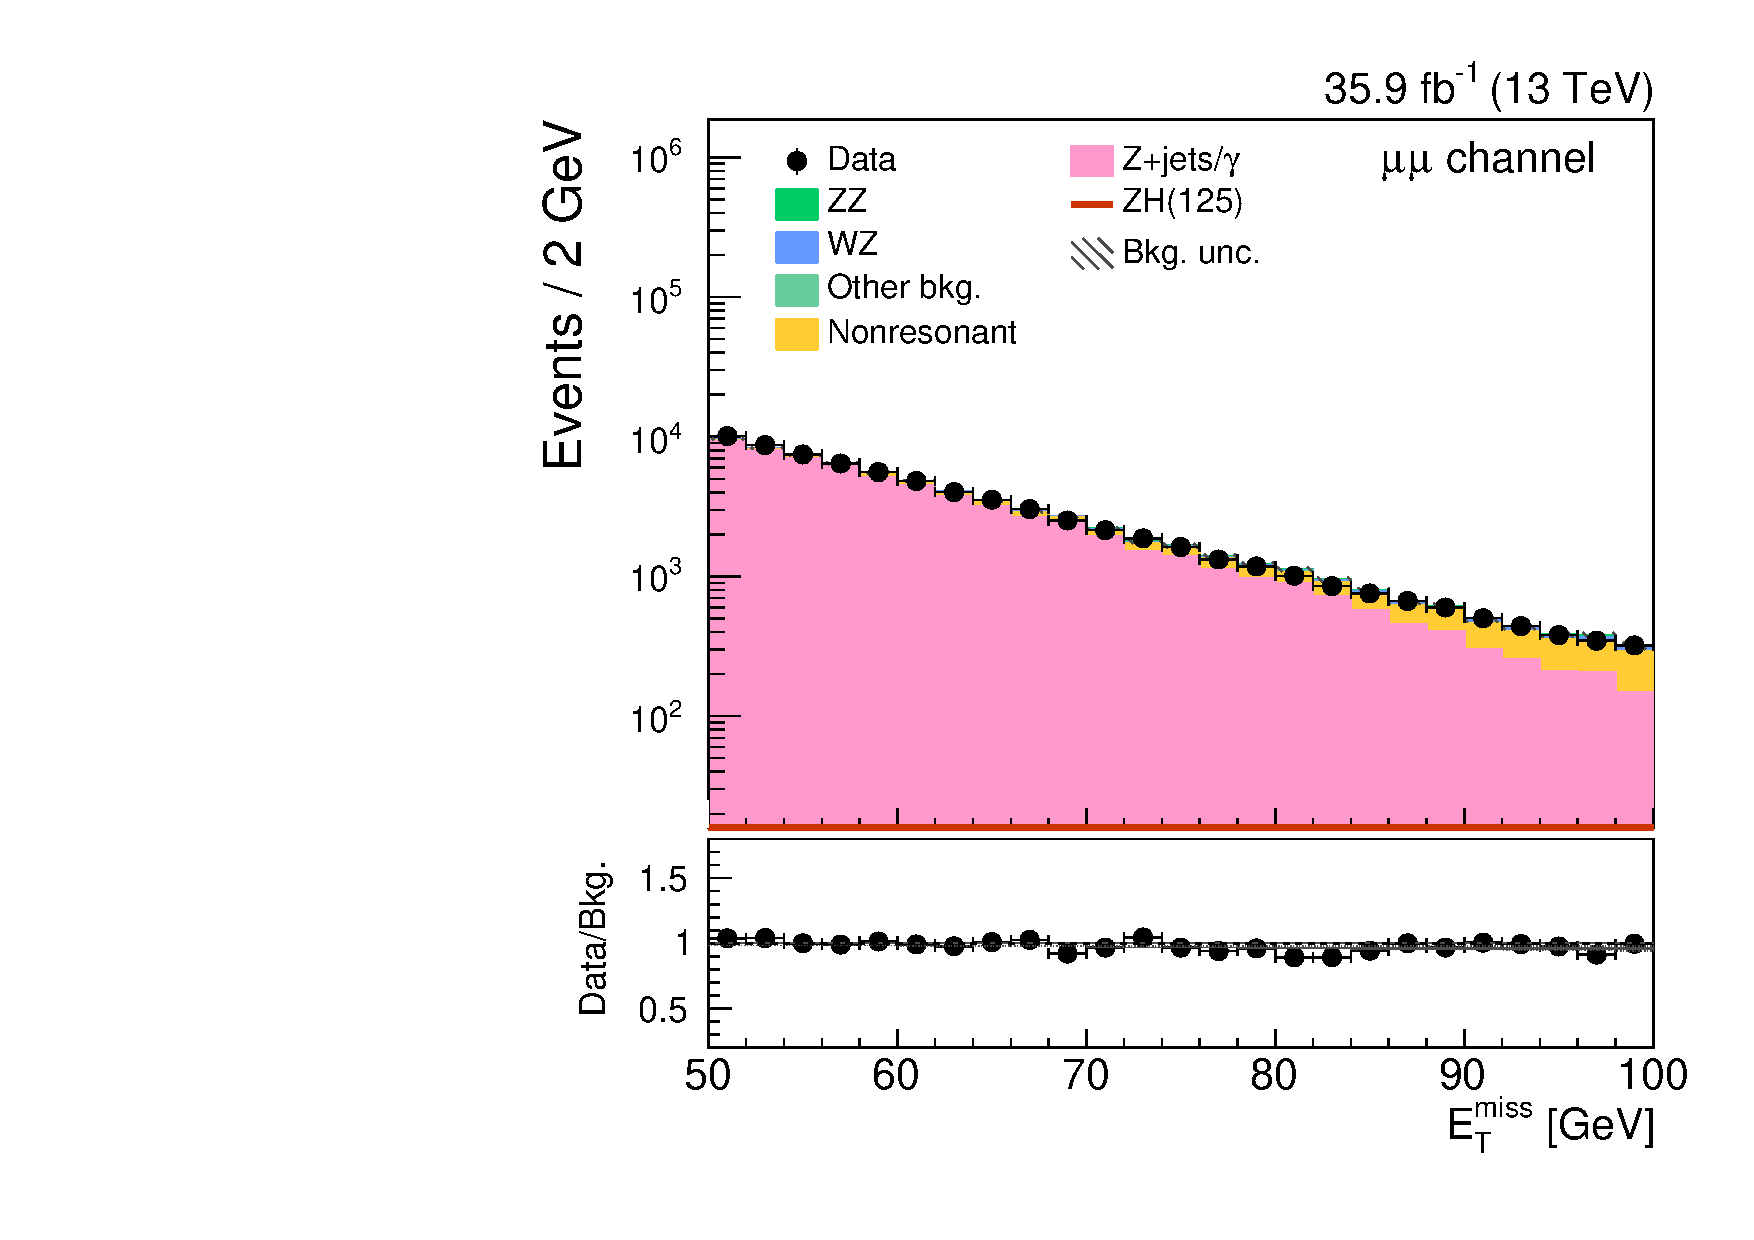
\includegraphics[width=\cmsFigWidth]{figures/presel_met_mm.pdf}
\caption{
  Distributions of the missing transverse energy for each flavor channel in $\zll$ events with $\pt^{\ell\ell} > 60~\GeV$ and $\met > 40~\GeV$.
  The uncertainty band corresponds to the statistical uncertainty only. Left: dielectron channel. Right: dimuon channel.
}
\label{fig:distributions_presel_met}
\end{center}
\end{figure}

\subsection{Signal selection}
\label{ss:zlldmsigsel}
After the preselection, more stringent criteria are applied to enhance the significance of a dark matter signal.
There are nonresonant background processes which do not have anything to do with a Z boson,
but they can end up looking like a signal event by way of combinatorics.
A great example of this is two independent objects each eventually producing a charged lepton and missing energy, such as leptonic WW decays.
Another example is top-quark backgrounds such as the ubiquitous ditop production.
There, each top-quark decays to a b-quark and a W boson, which decays leptonically.
These nonresonant backgrounds are already partially mitigated by the Z candidate mass window requirement in the preselection.
It can be further reduced by requiring a small angular separation of the leptons, $\Delta R < 1.8$.

All of the dark matter models considered are quark-induced processes 
with no extra quarks or gluons produced in the final state.
Refer to the diagrams in Figure~\ref{fig:BSMdiagrams}.
Hadronic activity in a dark matter signal event is minimal and only arises from the initial-state radiation of a gluon or secondary pileup interactions.
Top-quark backgrounds are not quark-induced, and produce b-jets from the top-quark decays as well as extra jets in general.
They are easily reduced by requiring that events have no more than one jet with $\pt^{j} > 30~\GeV$ and $|\eta|<2.4$.
Furthermore, a b-jet veto is imposed.
Events are rejected if a central jet is found which passes the ``Medium'' working point of the CSVv2 b-tagging algorithm ($>0.8484$).


\begin{figure}[!thbp]
 \centering
 \begin{tikzpicture}
  \begin{feynman}
   \vertex (g1) {\(\boldsymbol{g}\)};
   \vertex [below= 2cm of g1] (g2) {\(\boldsymbol{g}\)};
   \vertex [right= 2cm of g1] (a1);
   \vertex [right= 2cm of g2] (a2);
   \vertex [right= 1.5cm of a1] (b1);
   \vertex [right= 1.5cm of a2] (b2);
   \vertex [right= 1.5cm of b1] (c1);
   \vertex [right= 1.5cm of b2] (c2);
   \vertex [right= 1.5cm of c1] (e1);
   \vertex [right= 1.5cm of c2] (e2);
   \vertex [above= 0.3cm of e1] (f1) {\(\boldsymbol{\nu_{\ell}}\)};     
   \vertex [below= 0.3cm of e1] (f2) {\(\boldsymbol{\ell^{+}}\)};       
   \vertex [above= 0.3cm of e2] (f3) {\(\boldsymbol{\ell^{-}}\)};       
   \vertex [below= 0.3cm of e2] (f4) {\(\boldsymbol{\bar{\nu}_{\ell}}\)};
   \vertex [right= 1.0cm of b1] (e3);
   \vertex [above= 0.5cm of e3] (e5);
   \vertex [right= 1.0cm of b2] (e4);
   \vertex [below= 0.5cm of e4] (e6);
   
   \diagram* {
    (g1) -- [gluon, very thick] (a1),
    (g2) -- [gluon, very thick] (a2),
    (a2) -- [fermion, very thick] (a1),
    (a1) -- [fermion, very thick, edge label'=\(\boldsymbol{t}\)] (b1),
    (a2) -- [anti fermion, very thick, edge label=\(\boldsymbol{\bar{t}}\)] (b2),
    (b1) -- [boson, very thick, edge label'=\(\boldsymbol{\W^{+}}\)] (c1),
    (b2) -- [boson, very thick, edge label=\(\boldsymbol{\W^{-}}\)] (c2),
    (c1) -- [fermion, very thick] (f1),
    (c1) -- [anti fermion, very thick] (f2),
    (c2) -- [fermion, very thick] (f3),
    (c2) -- [anti fermion, very thick] (f4),
    (b1) -- [fermion, very thick, edge label=\(\boldsymbol{b}\)] (e5),
    (b2) -- [anti fermion, very thick, edge label'=\(\boldsymbol{\bar{b}}\)] (e6),
   };
  \end{feynman}
 \end{tikzpicture} \hspace{1cm}
 \begin{tikzpicture}
  \begin{feynman}
   \vertex (q1) {\(\boldsymbol{\Pq}\)};
   \vertex [below= 2cm of q1] (q2) {\(\boldsymbol{\Paq}\)};
   \vertex [right= 2cm of q1] (a);
   \vertex [right= 2cm of q2] (b);
   \vertex [right= 2cm of a] (c);
   \vertex [right= 2cm of b] (d);
   \vertex [right= 1.5cm of c] (e);
   \vertex [right= 1.5cm of d] (f);
   \vertex [above= 0.3cm of e] (f1) {\(\boldsymbol{\ell^{-}}\)};
   \vertex [below= 0.3cm of e] (f2) {\(\boldsymbol{\bar{\nu}_{\ell}}\)};
   \vertex [above= 0.3cm of f] (f3) {\(\boldsymbol{\nu_{\ell}}\)};
   \vertex [below= 0.3cm of f] (f4) {\(\boldsymbol{\ell^{+}}\)};
   
   \diagram* {
    (q1) -- [fermion, very thick] (a),
    (q2) -- [anti fermion, very thick] (b),
    (a) -- [fermion, very thick] (b),
    (a) -- [boson, very thick, edge label'=\(\boldsymbol{\W^{-}}\)] (c),
    (b) -- [boson, very thick, edge label'=\(\boldsymbol{\W^{+}}\)] (d),
    (c) -- [fermion, very thick] (f1),
    (c) -- [anti fermion, very thick] (f2),
    (d) -- [fermion, very thick] (f3),
    (d) -- [anti fermion, very thick] (f4),
   };
  \end{feynman}
 \end{tikzpicture} 
 \caption{Nonresonant backgrounds. Left: ditop production resulting in two b-jets, two charged leptons, and missing energy. Right: WW production producing two charged leptons and missing energy.}
 \label{fig:dmnrb}
\end{figure}

Events are rejected if a third, additional electron or muon is reconstructed with $\pt > 10~\GeV$ using a loose selection; 
or if they contain a reconstructed hadronically decaying $\tau$ lepton with $\pt>18\GeV$.
These criteria reduce the background contribution from $\W\Z$ events
where the lepton originating from the $\W$ boson decay is not reconstructed.

Last but not least, the Drell-Yan process must still be dealt with.
It is important to note that the Drell-Yan process cannot generate real missing energy.
It can only look like a signal event due to detector acceptance effects and mismeasurement of jets.
This is handled in the signal selection in several ways.
The Z candidate and the missing transverse energy are required to be back-to-back in the transverse plane: $\Delta \phi_{\ell\ell,\met} > 2.6$.
Their momenta in the transverse plane must also be balanced\footnote{This is frequently referred to as ``the balance.''}: $|\met-\pt^{\ell\ell}|/\pt^{\ell\ell} < 0.4$.
A mismeasurement of an energetic jet will induce missing energy in the same angular direction of the jet.
So if there is a jet in the event, it must not be in the same azimuthal direction as the jet: $\Delta \phi_{{\rm jet},\met} > 0.5~ \mathrm{Rad}$.
This also helps deal with the aforementioned lost WZ, in the case that the lepton is
mistakenly reconstructed as a jet or the $\tau$ lepton reconstruction fails.
Finally, since the missing energy distribution of the Drell-Yan background is a sharply falling spectrum,
events must have $\met$ larger than 100 \GeV.

A summary of the criteria for the signal region are given in Table~\ref{tab:zlldmsigsel}.
Following this selection, a dark matter signature could, in principle, appear prominently in the spectrum of missing transverse energy.
A maximum likelihood fit is performed to test the compatibility of the observed spectrum with signal+background and background-only hypotheses.
The likelihood is described below in Section~\ref{sec:likelihood}.

\begin{table}[hbtp]
  \begin{center}
 {\scriptsize
  \begin{tabular} {lcc}
\hline
  Variable & Selection  & Rejection Target \\
\hline
$N_{\ell}$                                & == 2                                         & $\W\Z$, $\V\V\V$      \\
\multirow{2}{*}{$\pt^{\ell}$}             & $>$25/20\GeV (electrons)                     & QCD \\
                                          & $>$20\GeV (muons)                            & QCD  \\
$\Z$ boson requirement ($\GeV$)           & $\left|\mll-m_{\Z}\right| < 15\GeV$          & $\W\W$, top-quark         \\
Jet counting                              & $\leq$ 1 jet with $\pt^{\rm j} > 30~\GeV$    & $\dyll$, top-quark, $\V\V\V$ \\
$\pt^{\ell\ell}$ ($\GeV$)                 & $>$ 60                                       & $\dyll$           \\
B-tagging veto                            & CSVv2 $<$ 0.8484                             & Top-quark, $\V\V\V$   \\
Tau veto                                  & 0 $\Pgt_{\rm h}$ candidates with $\pt^{\Pgt}>18\GeV$ & $\W\Z$   \\
$\met$  ($\GeV$)                          & $>$ 100                                      & $\dyll$, $\W\W$, top-quark   \\
$\Delta \phi_{\ell\ell,\met}$             & $>$ 2.6                                      & $\dyll$           \\
$|\met-\pt^{\ell\ell}|/\pt^{\ell\ell}$    & $<$ 0.4                                      & $\dyll$             \\
$\Delta \phi_{{\rm jet},\met}$            & $>$ 0.5                                      & $\dyll$, $\W\Z$         \\
$\Delta R_{\ell\ell}$                     & $<$ 1.8                                      & $\W\W$, top-quark       \\
  \hline
  \end{tabular}
}
  \caption{Summary of the kinematic selection requirements for the $\met$-based analysis.}
  \label{tab:zlldmsigsel}
  \end{center}
\end{table}

\clearpage
\begin{figure}[!htb]
\centering
\setlength{\fboxsep}{0pt}
\setlength{\fboxrule}{0.3pt}
\fbox{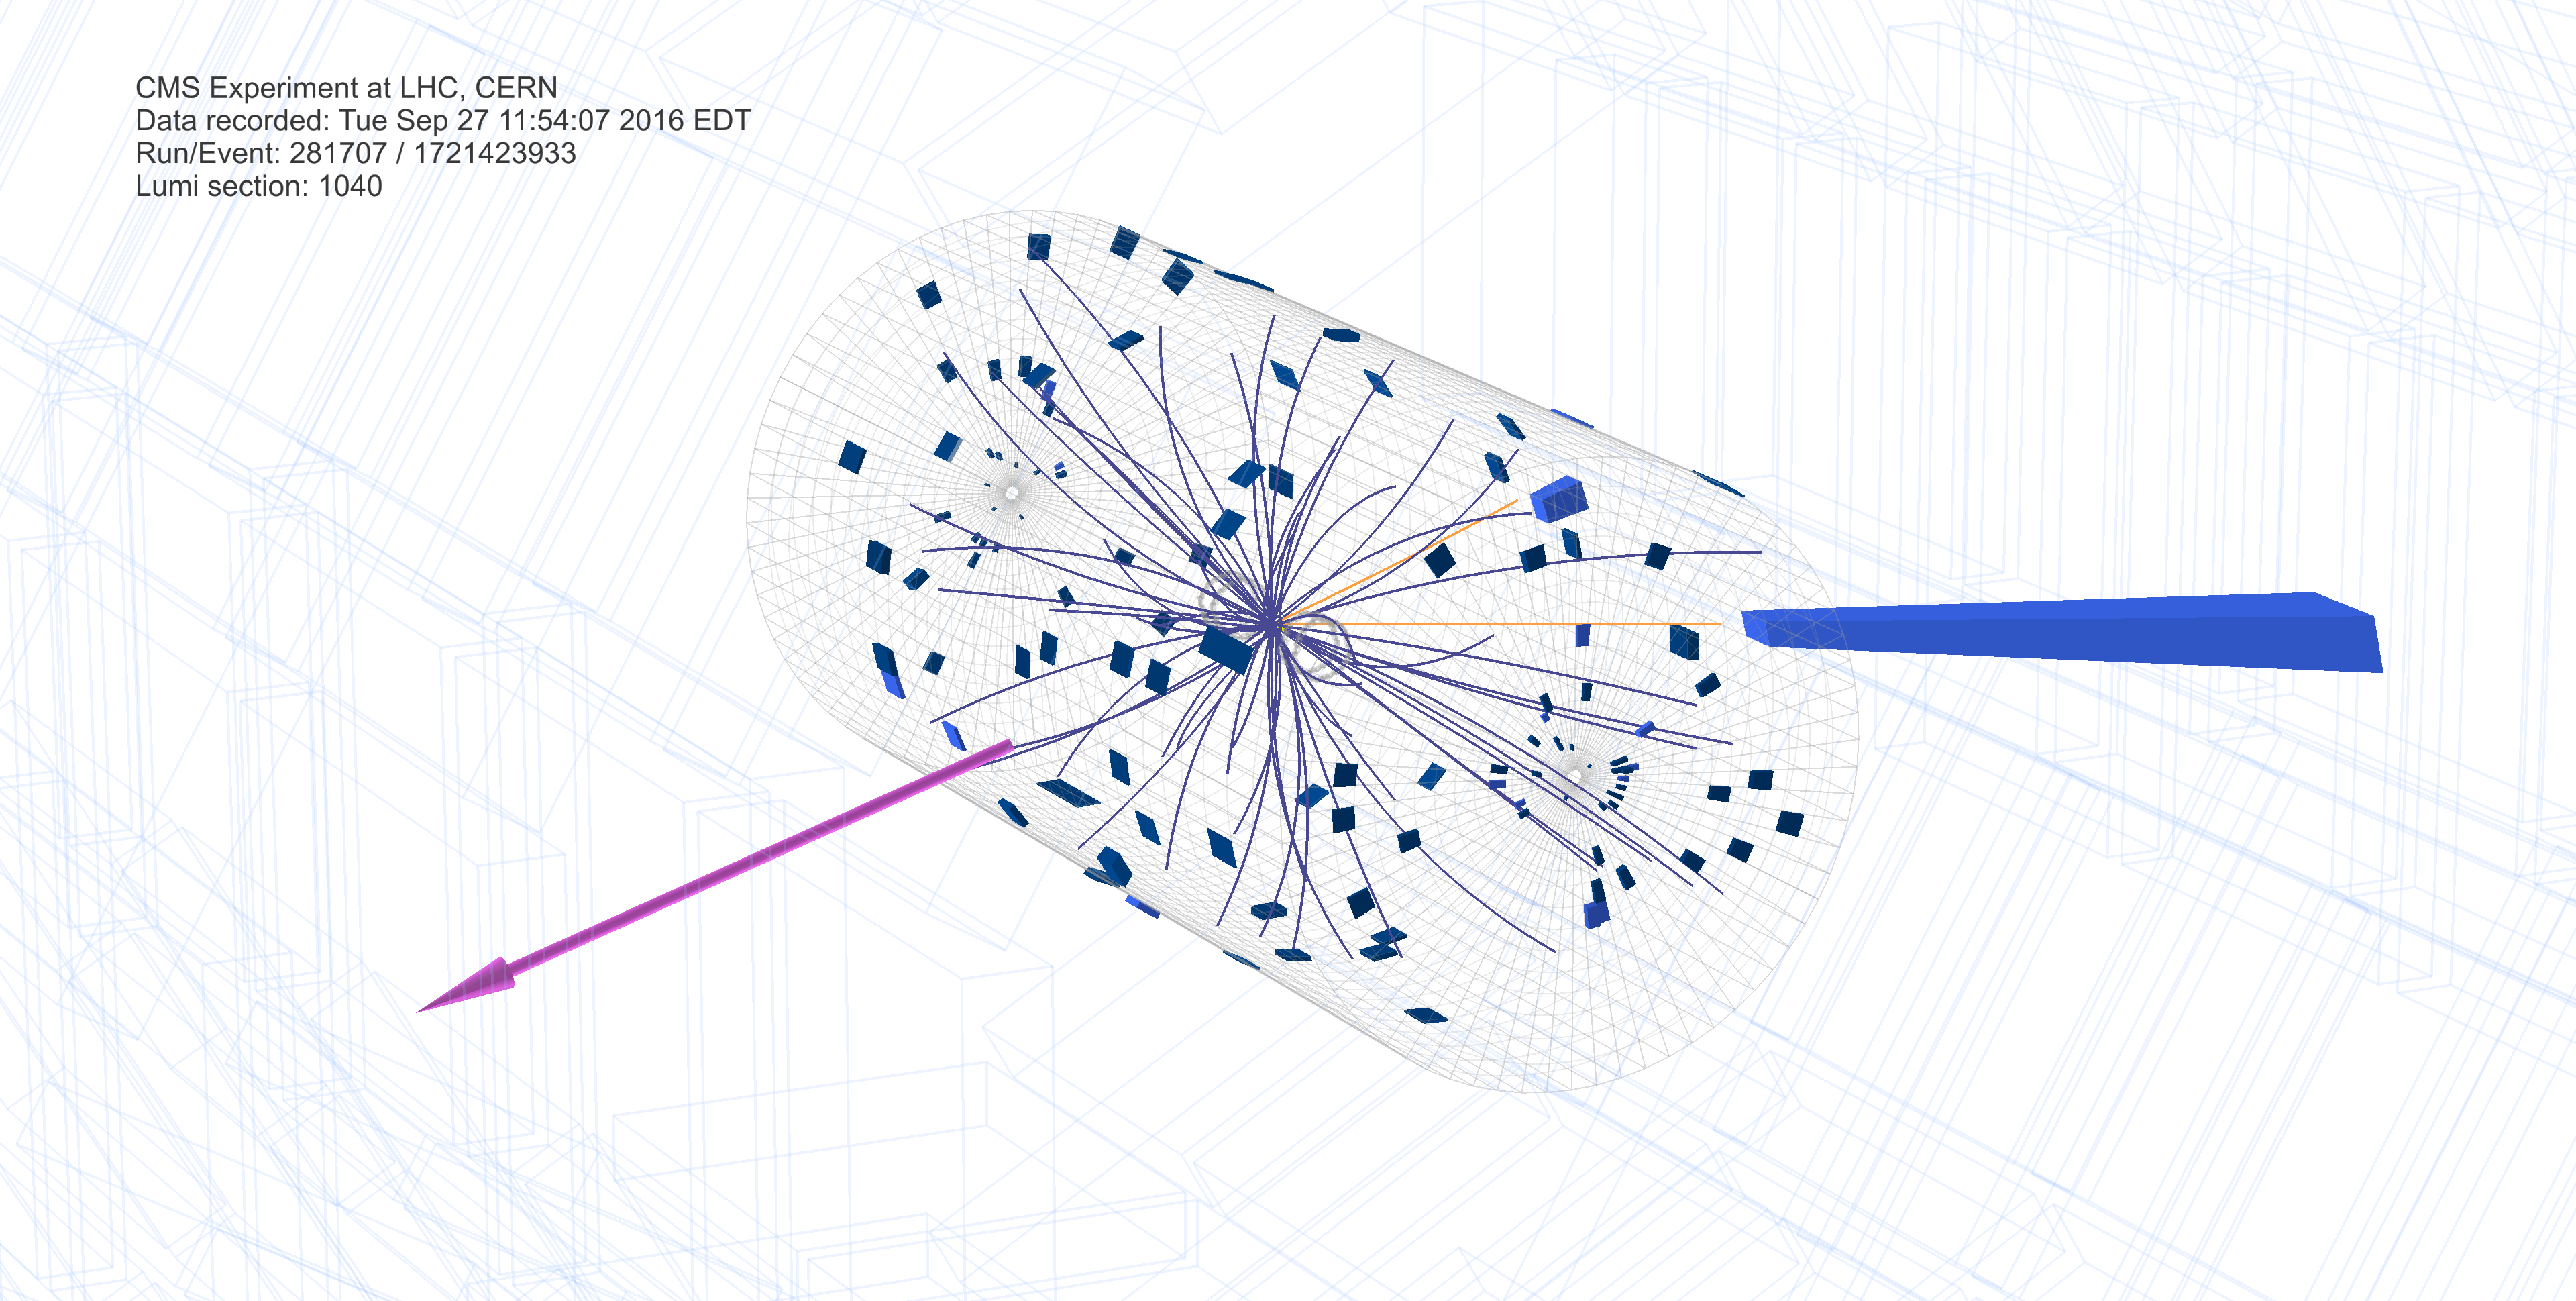
\includegraphics[width=1.0\textwidth]{figures/cmsShow_ZeeMET_MET300-281707_1721423933_1040_3DTower.png}}\vspace{1cm}

\fbox{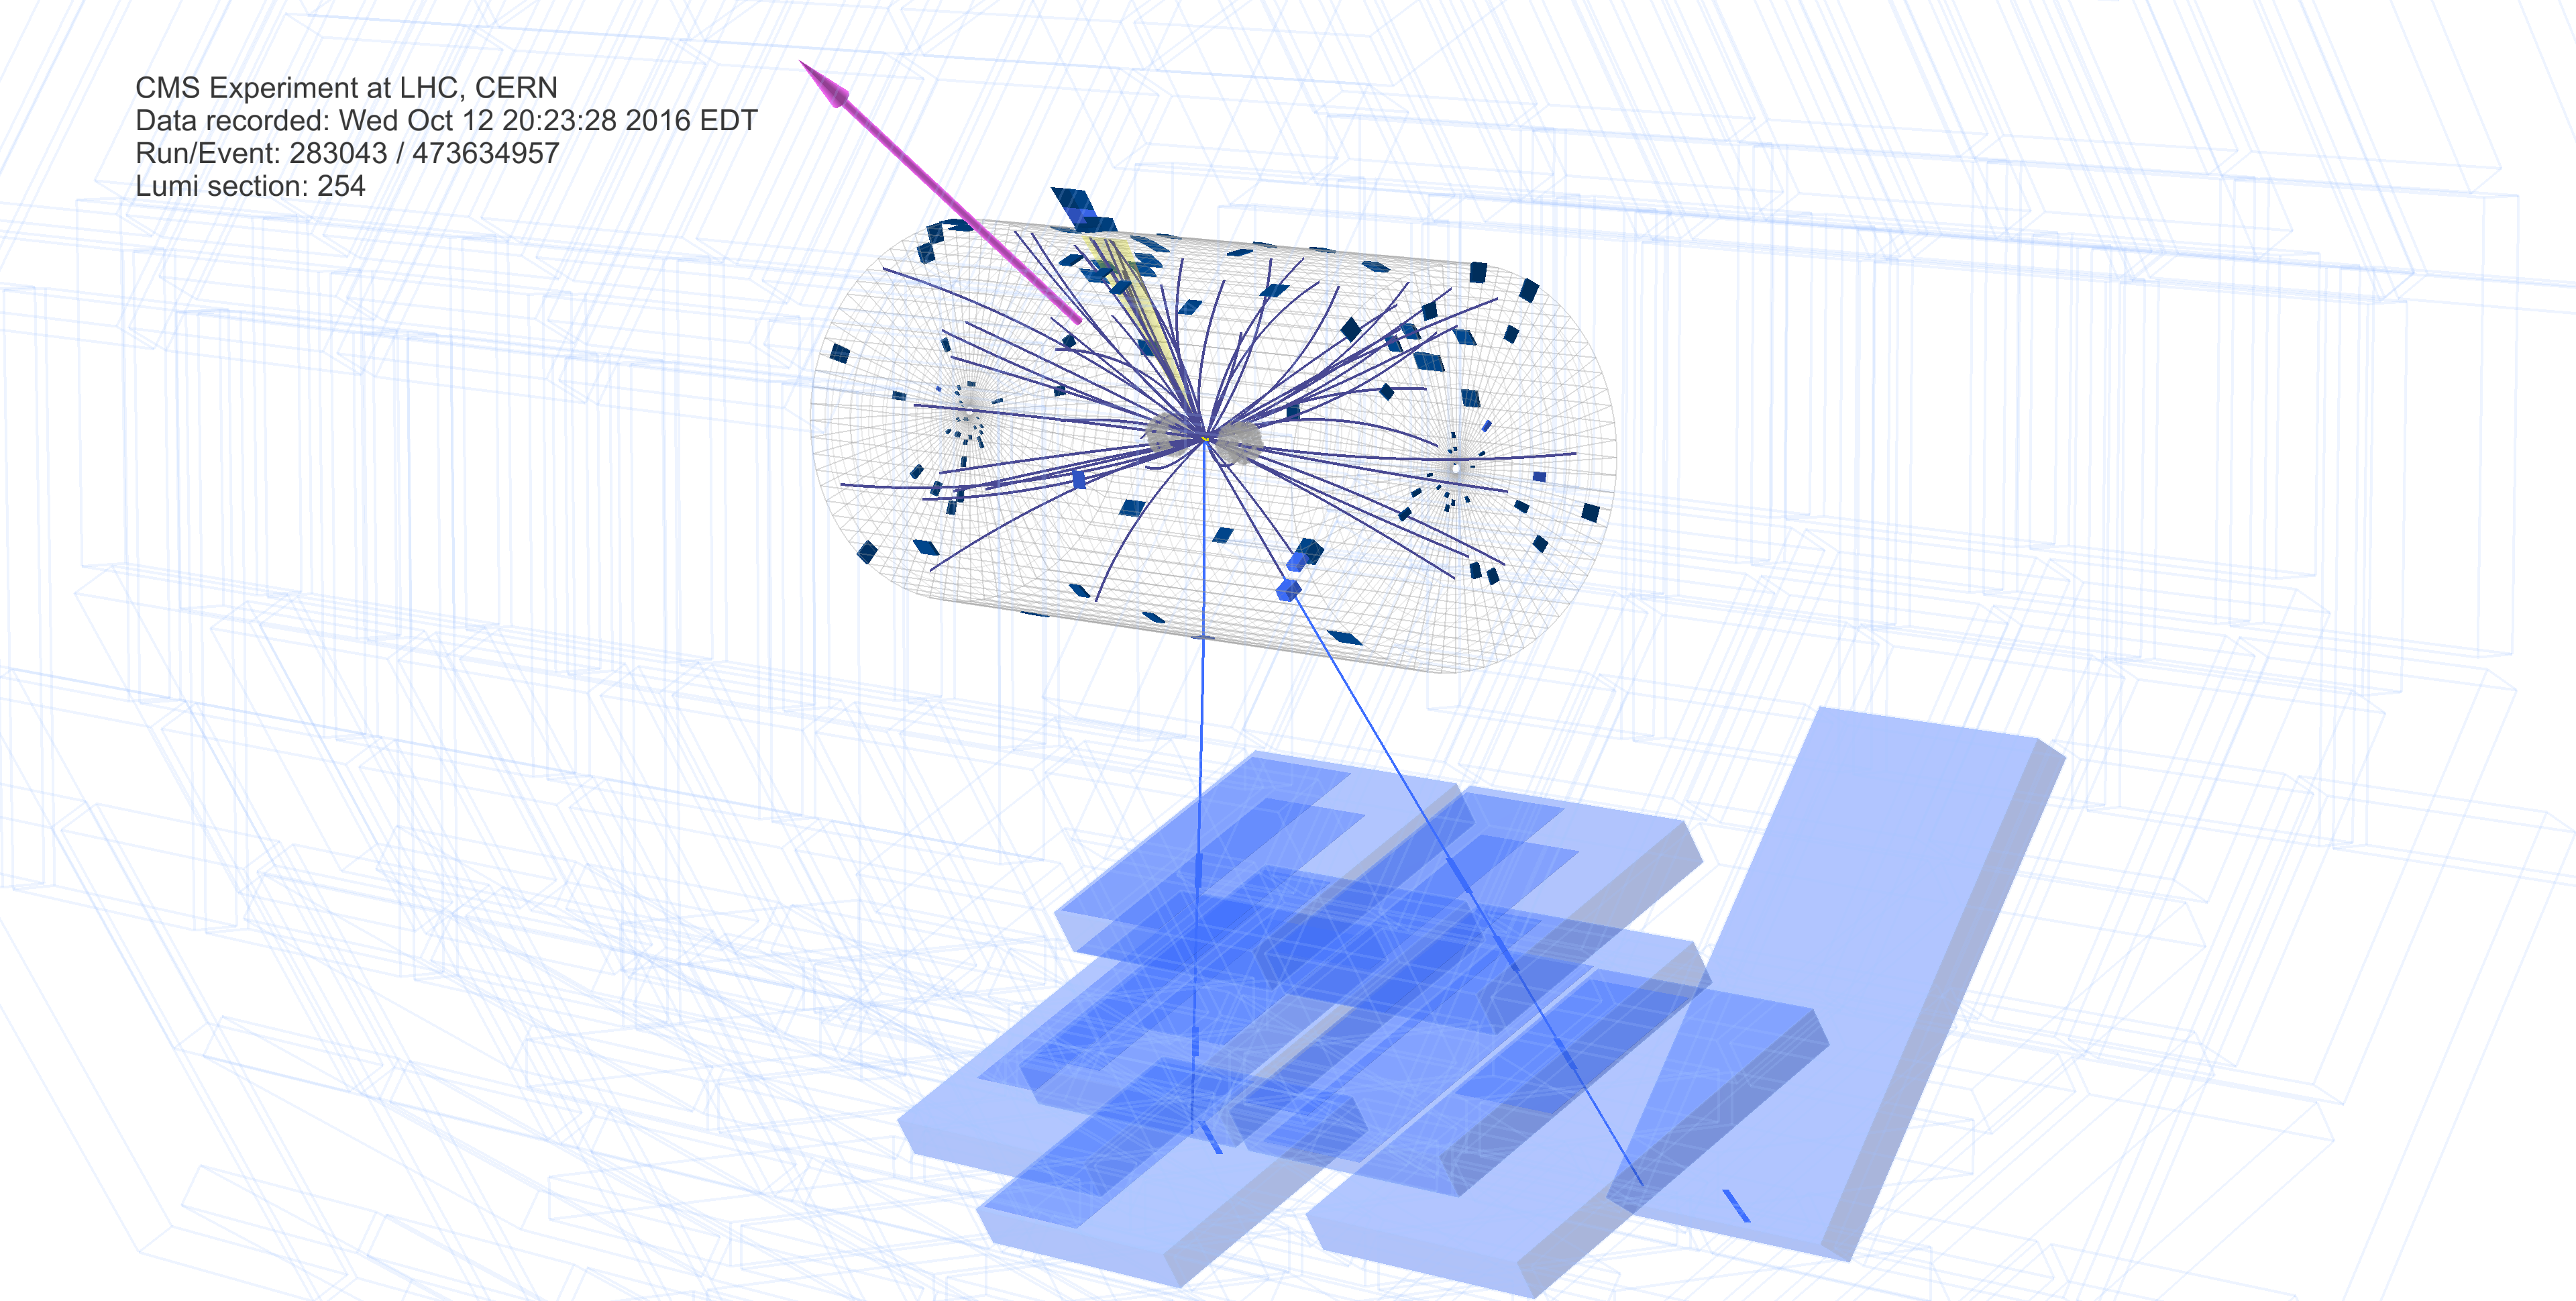
\includegraphics[width=1.0\textwidth]{figures/cmsShow_ZmmMET_MET300-283043_473634957_254_3DTower.png}}\vspace{1cm}

\caption{3D event displays of Z($\ell\ell$) events with $\met > 300 \GeV$.
\eventDisplayCaption
\label{fig:zllmet_eventdisplay}}
\end{figure}
\clearpage

%\clearpage
\section{Background estimation}
\label{sec:dmbkg}
A combination of data-driven methods and detailed simulated studies is used to
estimate background contributions.
The spectra of diboson processes are taken from simulation with conservative systematic uncertainties, but the ratio of ZZ/WZ is measured from data.
The nonresonant background processes may just as well produce different-flavor lepton pairs, so we extrapolate from those data events to estimate the yield of same-flavor lepton pairs.
The Drell-Yan process is estimated from a sideband of low $\met$. Its contribution for higher values of $\met$ is very small, but in order to verify the accurate simulation of the $\met$ spectrum, several cross-checks are performed.


%%%%%%%%%%%

\subsection{Diboson processes}
\label{sec:vvbkg}
Contributions from the ZZ and WZ processes are estimated from control regions in data.
These processes contribute to the signal region via the
$\ZZ\rightarrow\Lep\Lep\nu\nu$ and $\WZ\rightarrow\Lep\Lep\Lep\nu$ decay modes, respectively.
In both cases, the observed $\met$ corresponds to the \pt of one of the bosons.
The processes are estimated from the control samples described in Chapter~\ref{chap:dibosons}, Sections~\ref{sec:wz3l} and~\ref{sec:zz4l}. 
The visible decay modes allow us to probe the boson \pt distribution, which is expected to be independent of the decay mode.

Using the pure control samples with three or four leptons, an extrapolation is performed
to the missing energy spectra for $\Z\Z$ and $\W\Z$ events 
with only two reconstructed leptons and missing energy in the final state
\footnote{The $\W\Z$ process can appear this way due to a lost lepton, either from inefficiency in the reconstruction and identification or the non-hermetic tracking acceptance}.
Extrapolation to the $2\ell+\met$ final state is accomplished by furnishing a quantity
known as the emulated $\met$.
For the $\WZ$ process, the fake $\met$ is the true $\W$ boson $\pt$.
It is estimated by calculating the vectorial sum of the $\met$ vector and the transverse momentum vector of the third lepton.
For the $\Z\Z$ process, the fake $\met$ comes from taking the sum of any nominal true $\met$ and one of the leptonically-decaying $\Z$ bosons.
The $\Z$ boson which is made to vanish is chosen to be the one whose reconstructed 
mass is further from the nominal Z boson mass, previously denoted
as $\mathrm{Z}_2$ in Section~\ref{sec:zz4l}.
The choice of which Z candidate to use for the fake $\met$ is arbitrary,
and has almost no effect on the resulting distribution.

After the emulated \met procedure, the kinematic criteria of the selection in
Section~\ref{sec:zlldmsel} are applied.
The resulting emulated \met spectra are shown in Fig.~\ref{fig:histo_fakemet}.

\begin{figure}[htbp]
\centering
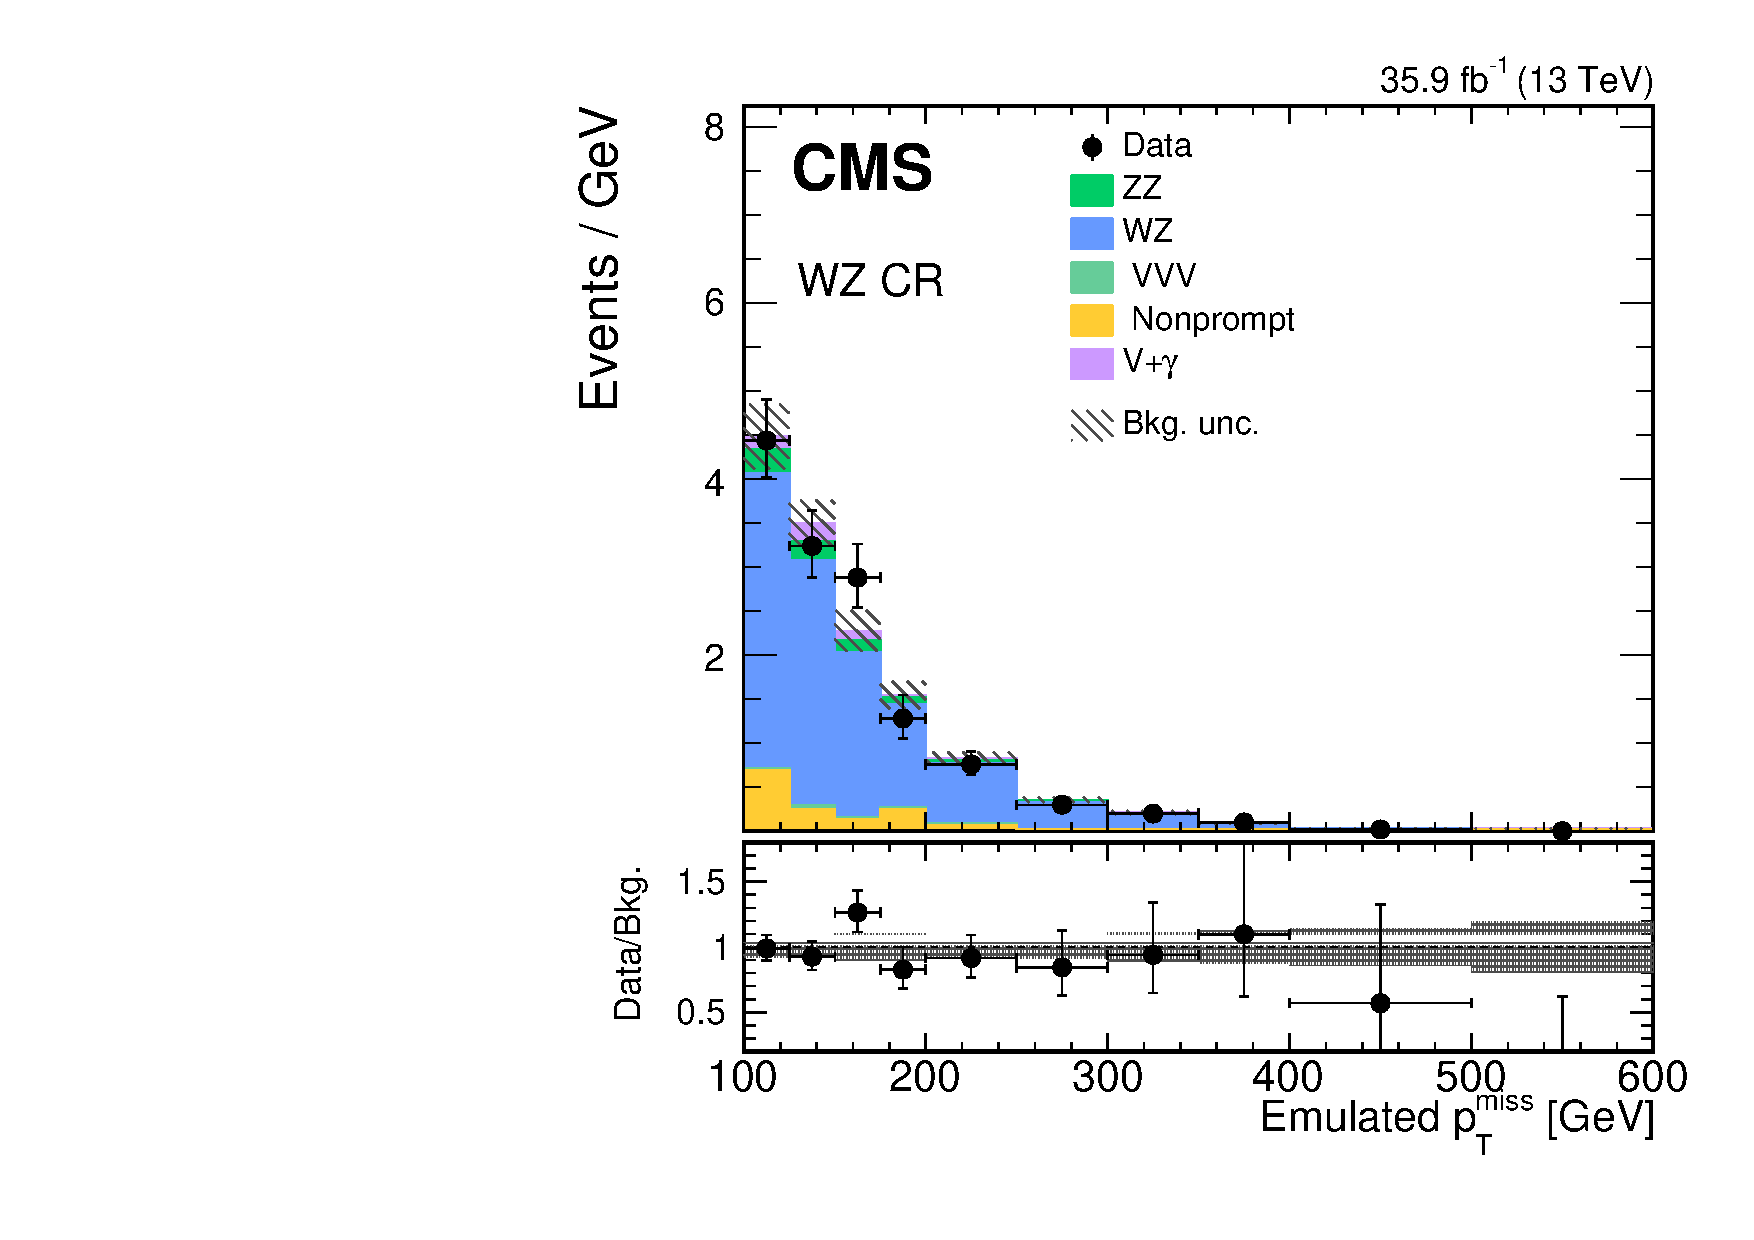
\includegraphics[width=0.48\textwidth]{figures/wz_fakemet_allcuts_postfit.pdf}
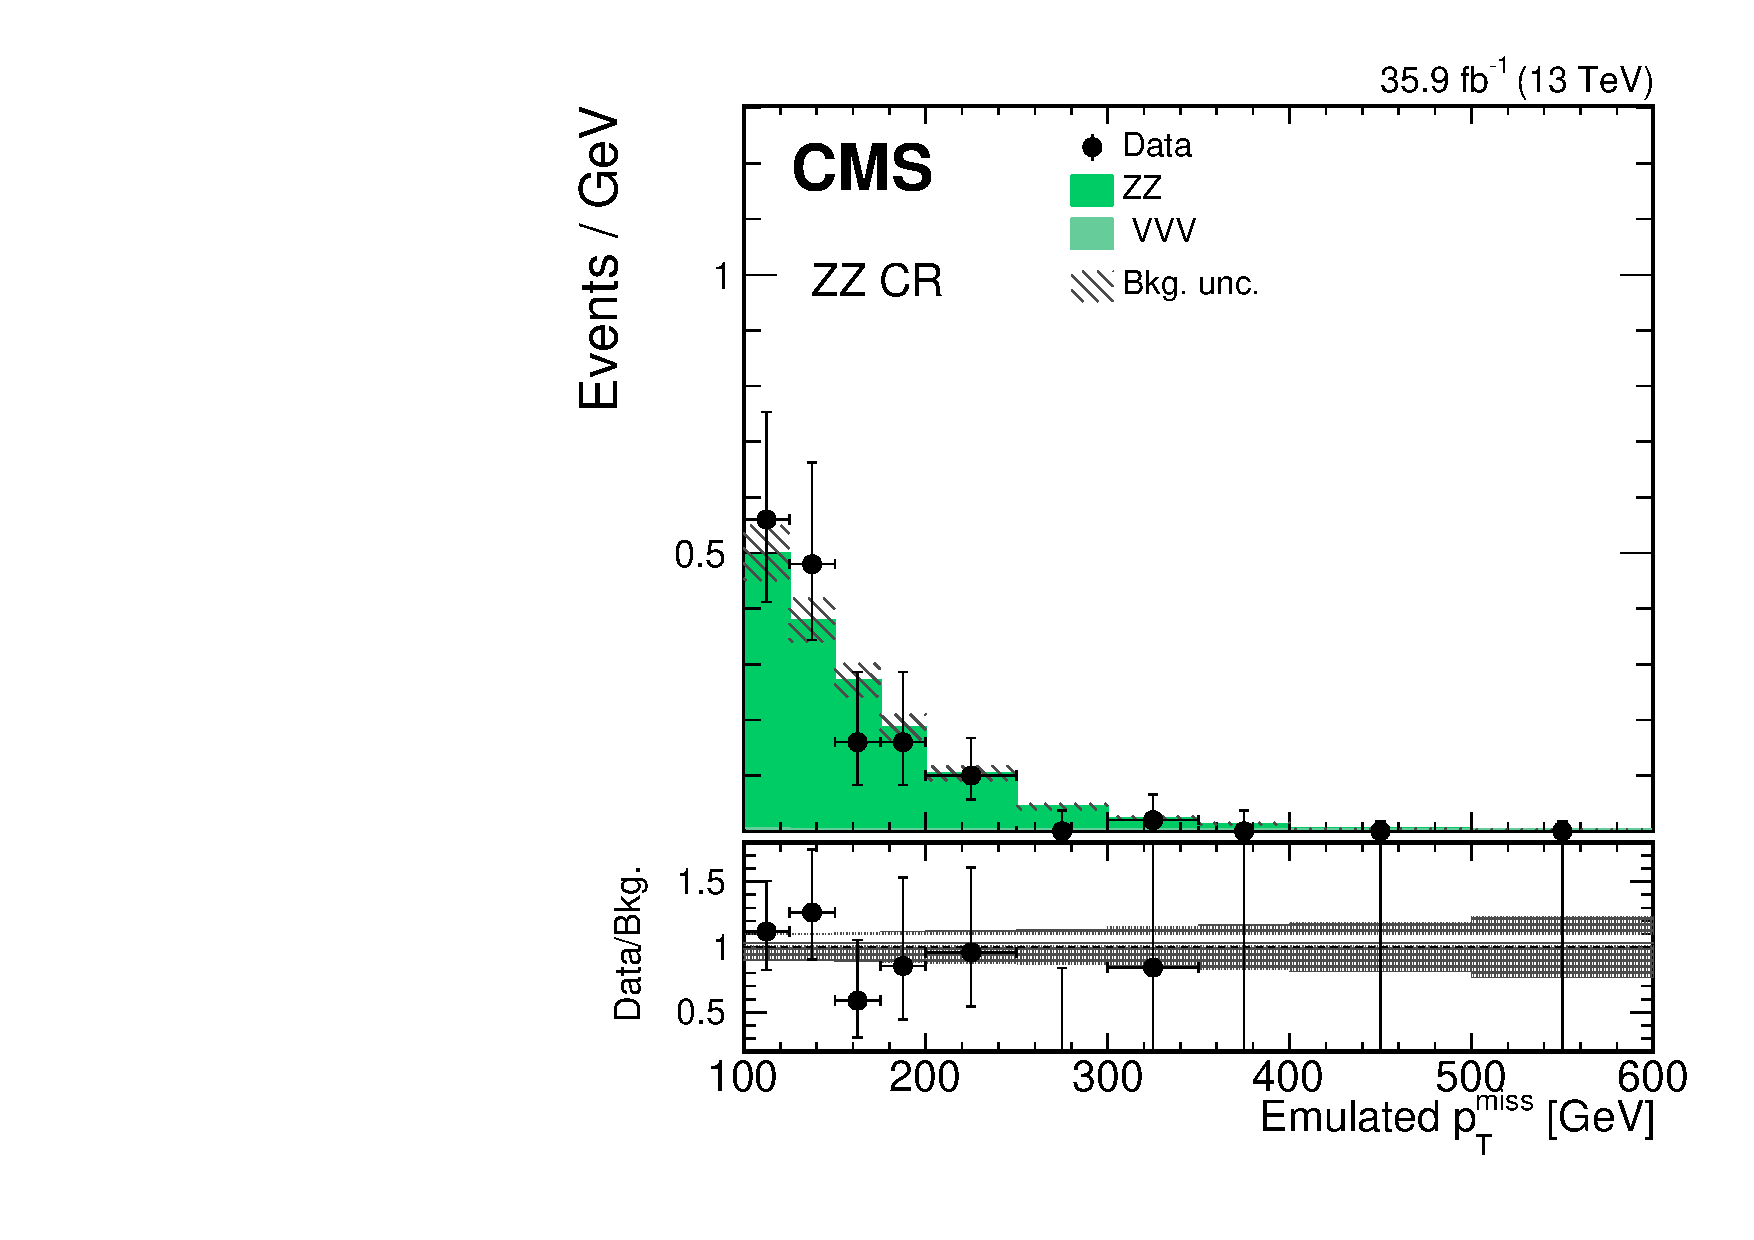
\includegraphics[width=0.48\textwidth]{figures/zz_fakemet_allcuts_postfit.pdf}
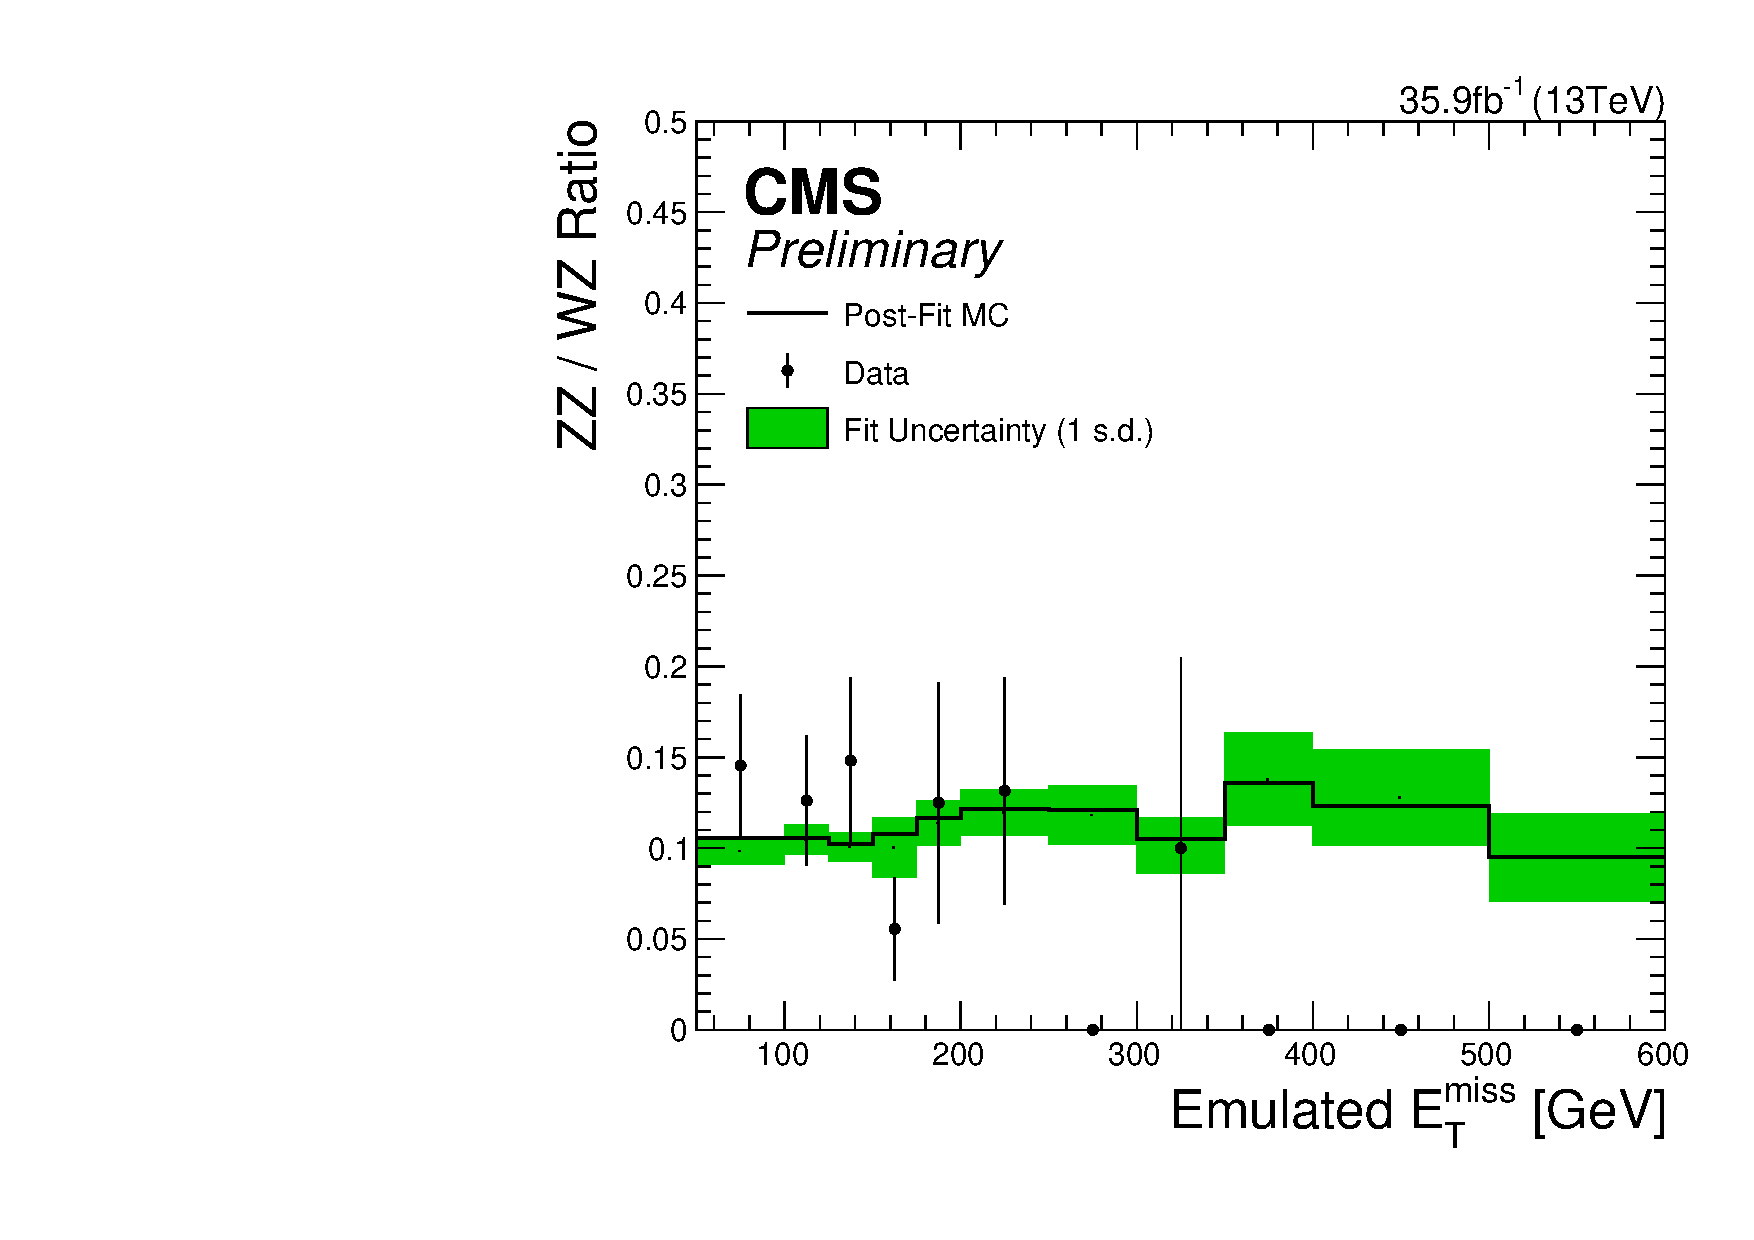
\includegraphics[width=0.48\textwidth]{figures/ratio_zzvswz.pdf}
\caption{Emulated $\met$
distribution for  the $\W\Z \to 3\Lep\nu$(top left) and $\Z\Z \to 4\Lep$ (top right)
control regions, and the ratio between both distributions in data and simulation (bottom).
Simulated distributions correspond to the result of the maximum likelihood fit described in Section~\ref{sec:likelihood}.
 Uncertainty bands correspond to both statistical and systematic uncertainty.}
\label{fig:histo_fakemet}
\end{figure}

\subsection{Nonresonant backgrounds}
\label{ss:dm_nrb}
The contribution of the nonresonant flavor symmetric backgrounds is estimated from a control
sample of events with dilepton of different flavors
($\Pe^{\pm}\Pgm^{\mp}$) that pass all analysis selections.
Nonresonant backgrounds (NRB) consists mainly of leptonic \PW\ decays in
$\ttbar$, $\cPqt\PW$ decays and 
$\PW\PW$ events. Small contributions from single top-quark events produced from
$s$-channel and $t$-channel processes, and $\cPZ\rightarrow \Pgt\Pgt$
events in which $\Pgt$ leptons produce light leptons and \ETm are also
considered in this NRB estimation. 

The method assumes the lepton flavor symmetry in the final states of these processes.
Since the leptonic decay branching ratios for the $ee$, $\mu\mu$ and $e\mu$ final states from NRB are 1:1:2,
the $e\mu$ events selected inside the $\Z$-mass window can be extrapolated to the $ee$ and $\mu\mu$ channels.
To account for differences in efficiency for electrons and muons, a correction factor $k_{ee}$ can be derived
by comparing the NRB yields in the $ee$ and $\mu\mu$ channels,
exactly as is done in Formulas~\ref{eq:kee} and~\ref{eq:nrb_xfer} from Section~\ref{sec:zptbkg}:

\begin{equation}
k_{ee} = \frac{\epsilon_e}{\epsilon_{\mu}} \approx \sqrt{\frac{N^{ee}_{NRB}}{N^{\mu\mu}_{NRB}}}
\end{equation}
once again under the assumption that each lepton leg acts independently.
In simulation, $k_{ee}$ is found to be about $0.88$ after all selection criteria are applied.
With this correction factor, the relation between the NRB yields in the signal and control region is:

\begin{equation}
\begin{split}
  N^{ee}_{NRB}     &= \frac{1}{2} k_{ee} N^{e\mu}_{NRB} \\
  N^{\mu\mu}_{NRB} &= \frac{1}{2} \frac{1}{k_{ee}} N^{e\mu}_{NRB} \\
\rightarrow N^{2\ell}_{NRB}  &= \frac{1}{2} \left( k_{ee} + \frac{1}{k_{ee}} \right) N^{e\mu}_{NRB} \\
&= f_{NRB} N^{e\mu}_{NRB}
\end{split}
\end{equation}
This transfer factor $f_{NRB}$ is implied by the MC estimates in the likelihood (Sec.~\ref{sec:likelihood}),
and the MC yields are found to be consistent with the derived relation within the statistical uncertainty.
Perturbations in the predicted transfer factor are suppressed upon summing the $ee+\mu\mu$ channels, as shown:
\begin{equation}
\begin{split}
  f + \delta f &= \frac{1}{2} \left( k + \delta k + \frac{1}{k + \delta k} \right) \\
  &= f + \frac{k^2-1}{2k^2} \delta k + \mathcal{O}(\delta^2) \\
  &= f + \mathcal{O}(\delta^2) \quad \text{for } k \approx 1
\end{split}
\end{equation}
such that the extrapolation uncertainty, taken as a conservative 20\%, covers any data-MC discrepancy
in the transfer factor.

Note that the $e\mu$ control sample contains a small contribution from
$\PW+{\mathrm{jets}}$ because of fake leptons. Since the rate of fake
electrons and muons is different, this method does not account
properly for the $\PW+{\mathrm{jets}}$ contribution, leading to an
underestimation of $\PW+{\mathrm{jets}}\to ee+X$, and an
overestimation of $\PW+{\mathrm{jets}}\to \mu\mu+X$. Given the very 
small yield expected for such process in the signal region, well below
the systematic uncertainty, the effect is neglected.
Moreover, the small biases resulting in the $ee$ and
$\mu\mu$ channels partially cancel out, so the overall effect on the
$\Lep\Lep$ channel is even smaller. 

As shown in Fig.~\ref{fig:m_em},
the $e\mu$ system mass, transverse momentum distributions and the \met\ distribution in
the $e\mu$ channel, the dominant sources in the $e\mu$ channel within
the Z mass window and in large $\ETm$ (or $p_{T}^{\Lep\Lep}$) region are
$\mathrm{t\bar{t}}, \ \mathrm{tW}, \ \mathrm{WW}, \ \mathrm{\tau\tau}$, and $\PW+{\mathrm{jets}}$ events.
Contributions from the $\mathrm{t\bar{t}Z}$ process
are deemed negligible.
As shown in Fig.~\ref{fig:met_tt_ww}, the shape of the $\met$ spectrum is identical in the $e\mu$ control region
and the $\ell\ell$ signal region.


\begin{figure}[hbtp]
 \begin{center}
   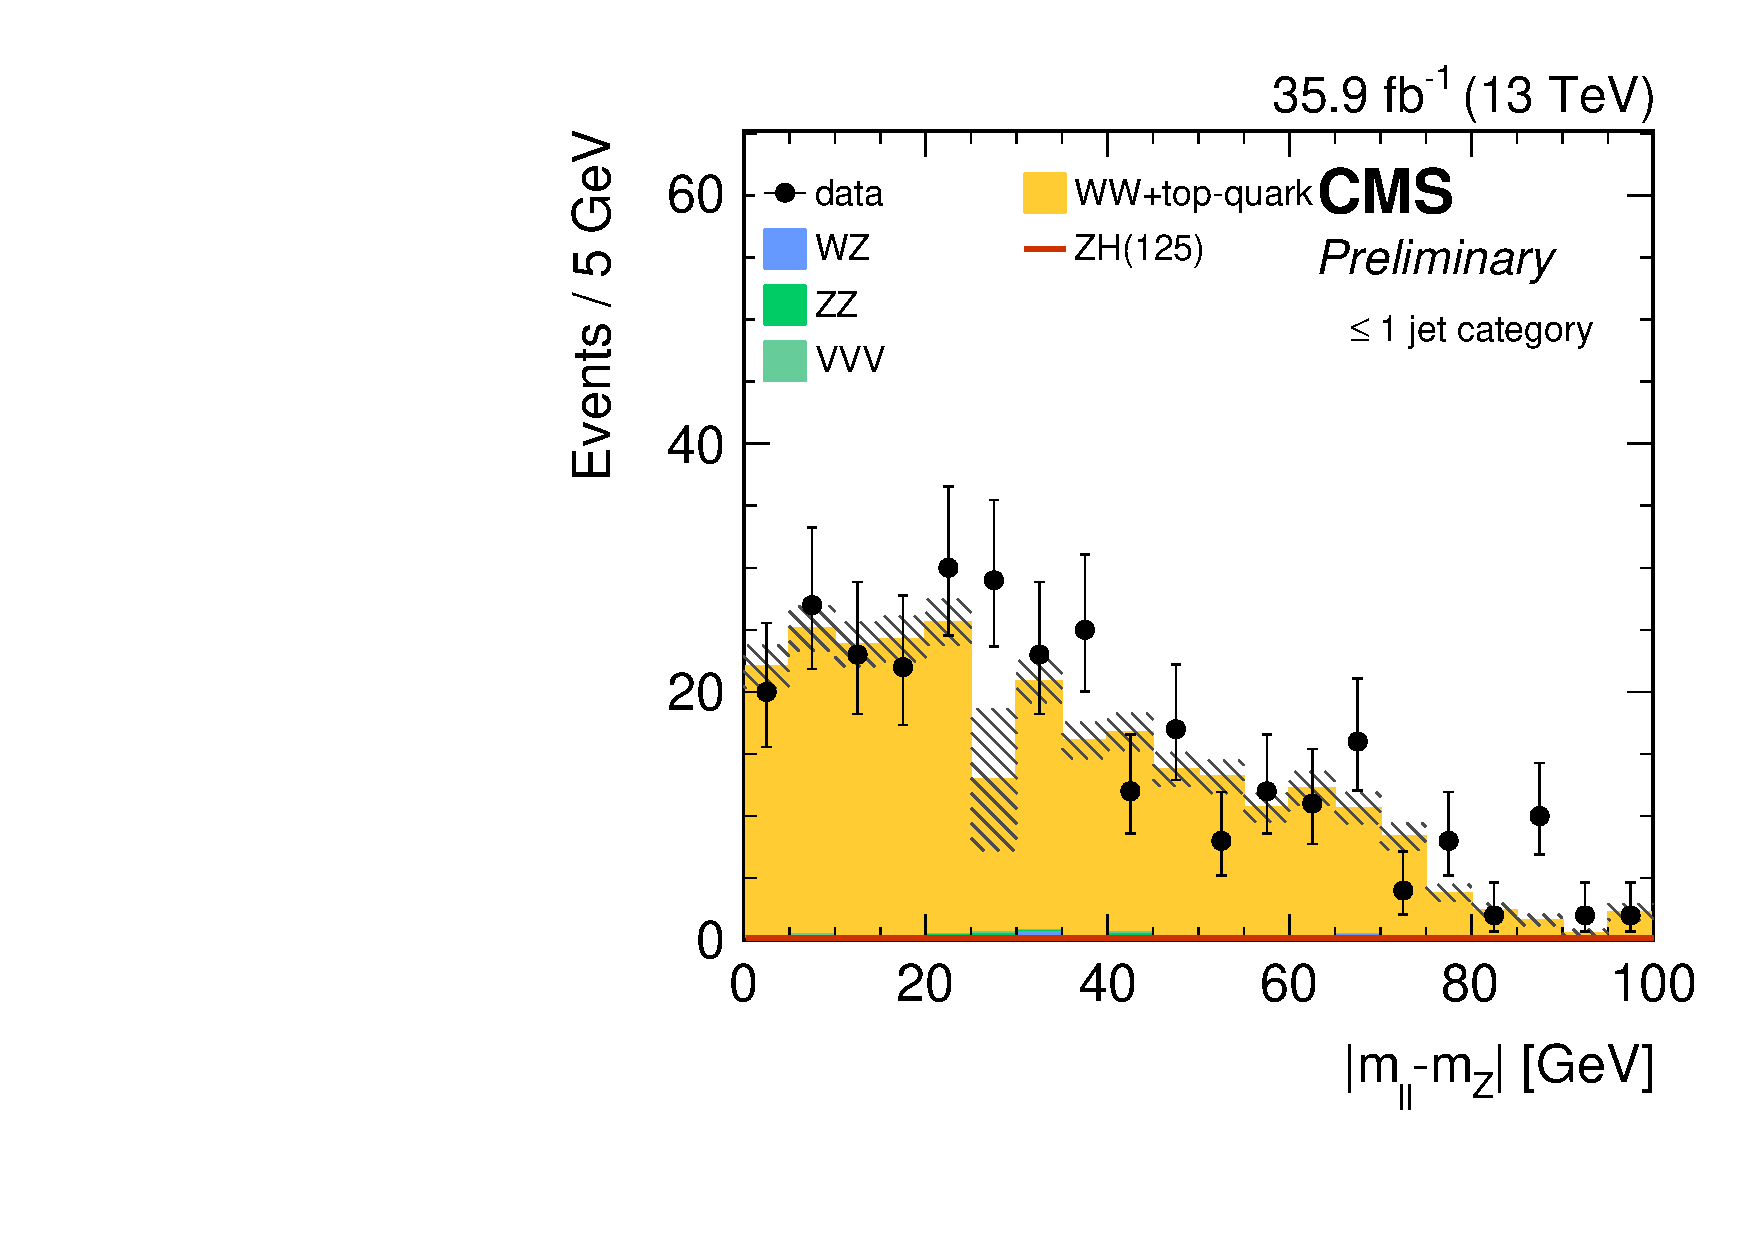
\includegraphics[width=0.46\textwidth]{figures/em_zh_1j_mll_allcutsbutone.pdf}
   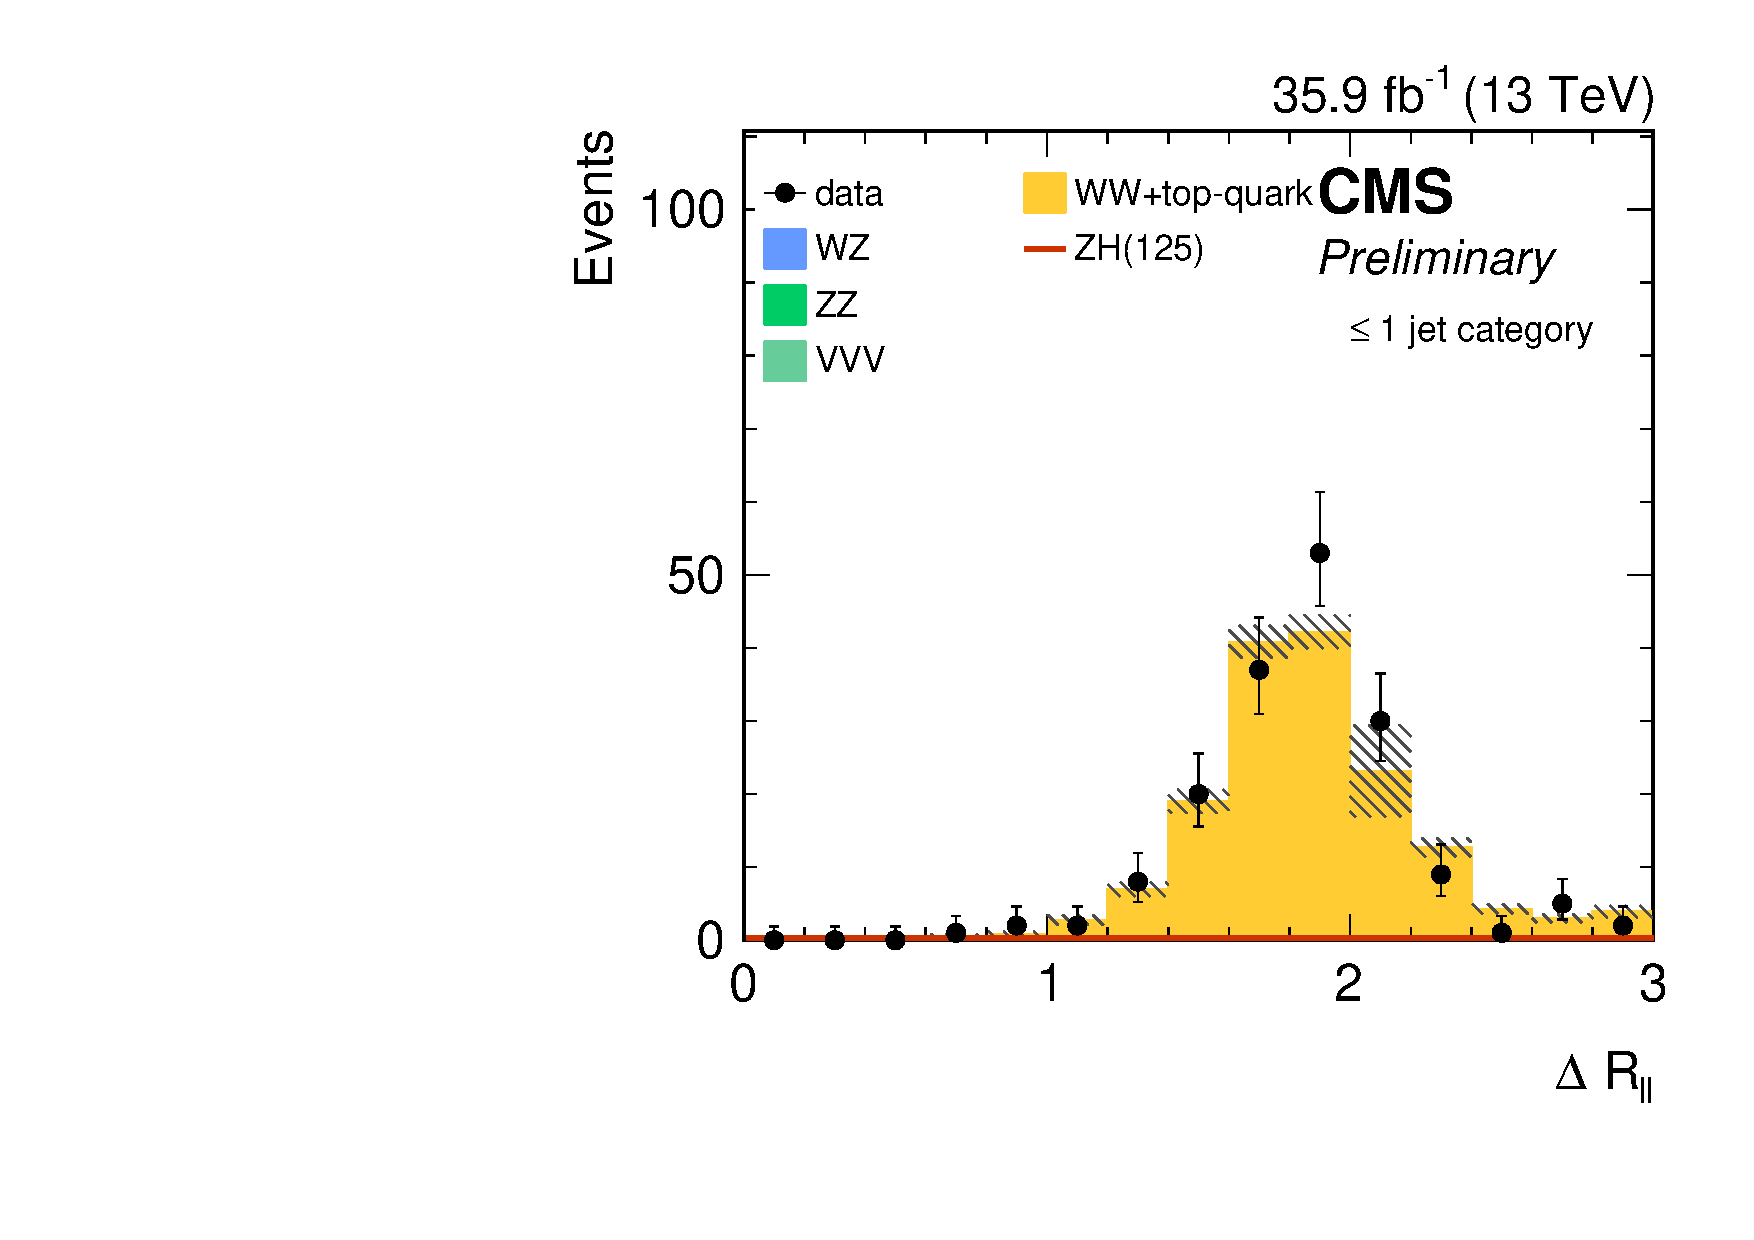
\includegraphics[width=0.46\textwidth]{figures/em_zh_1j_deltarll_allcutsbutone.pdf}\\
   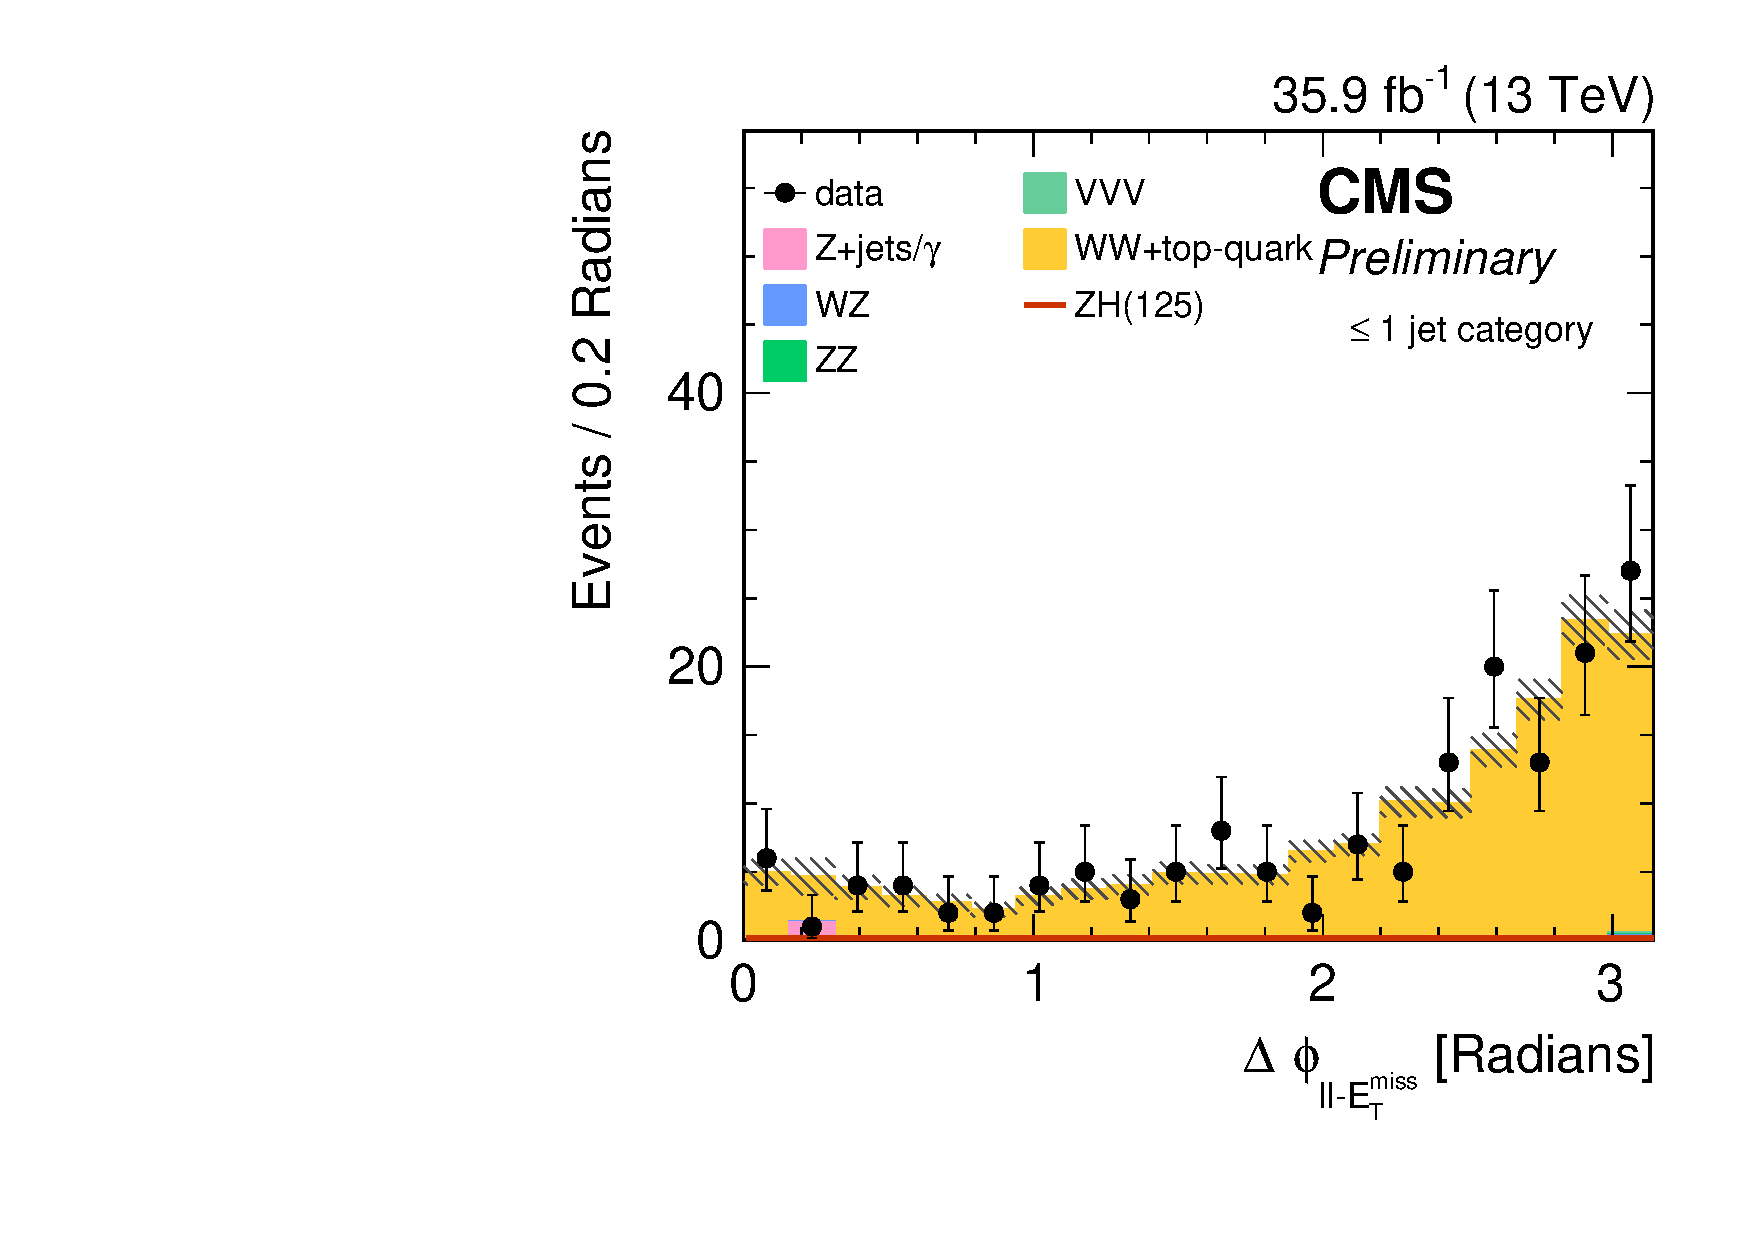
\includegraphics[width=0.46\textwidth]{figures/em_zh_1j_dphillmet_allcutsbutone.pdf}
   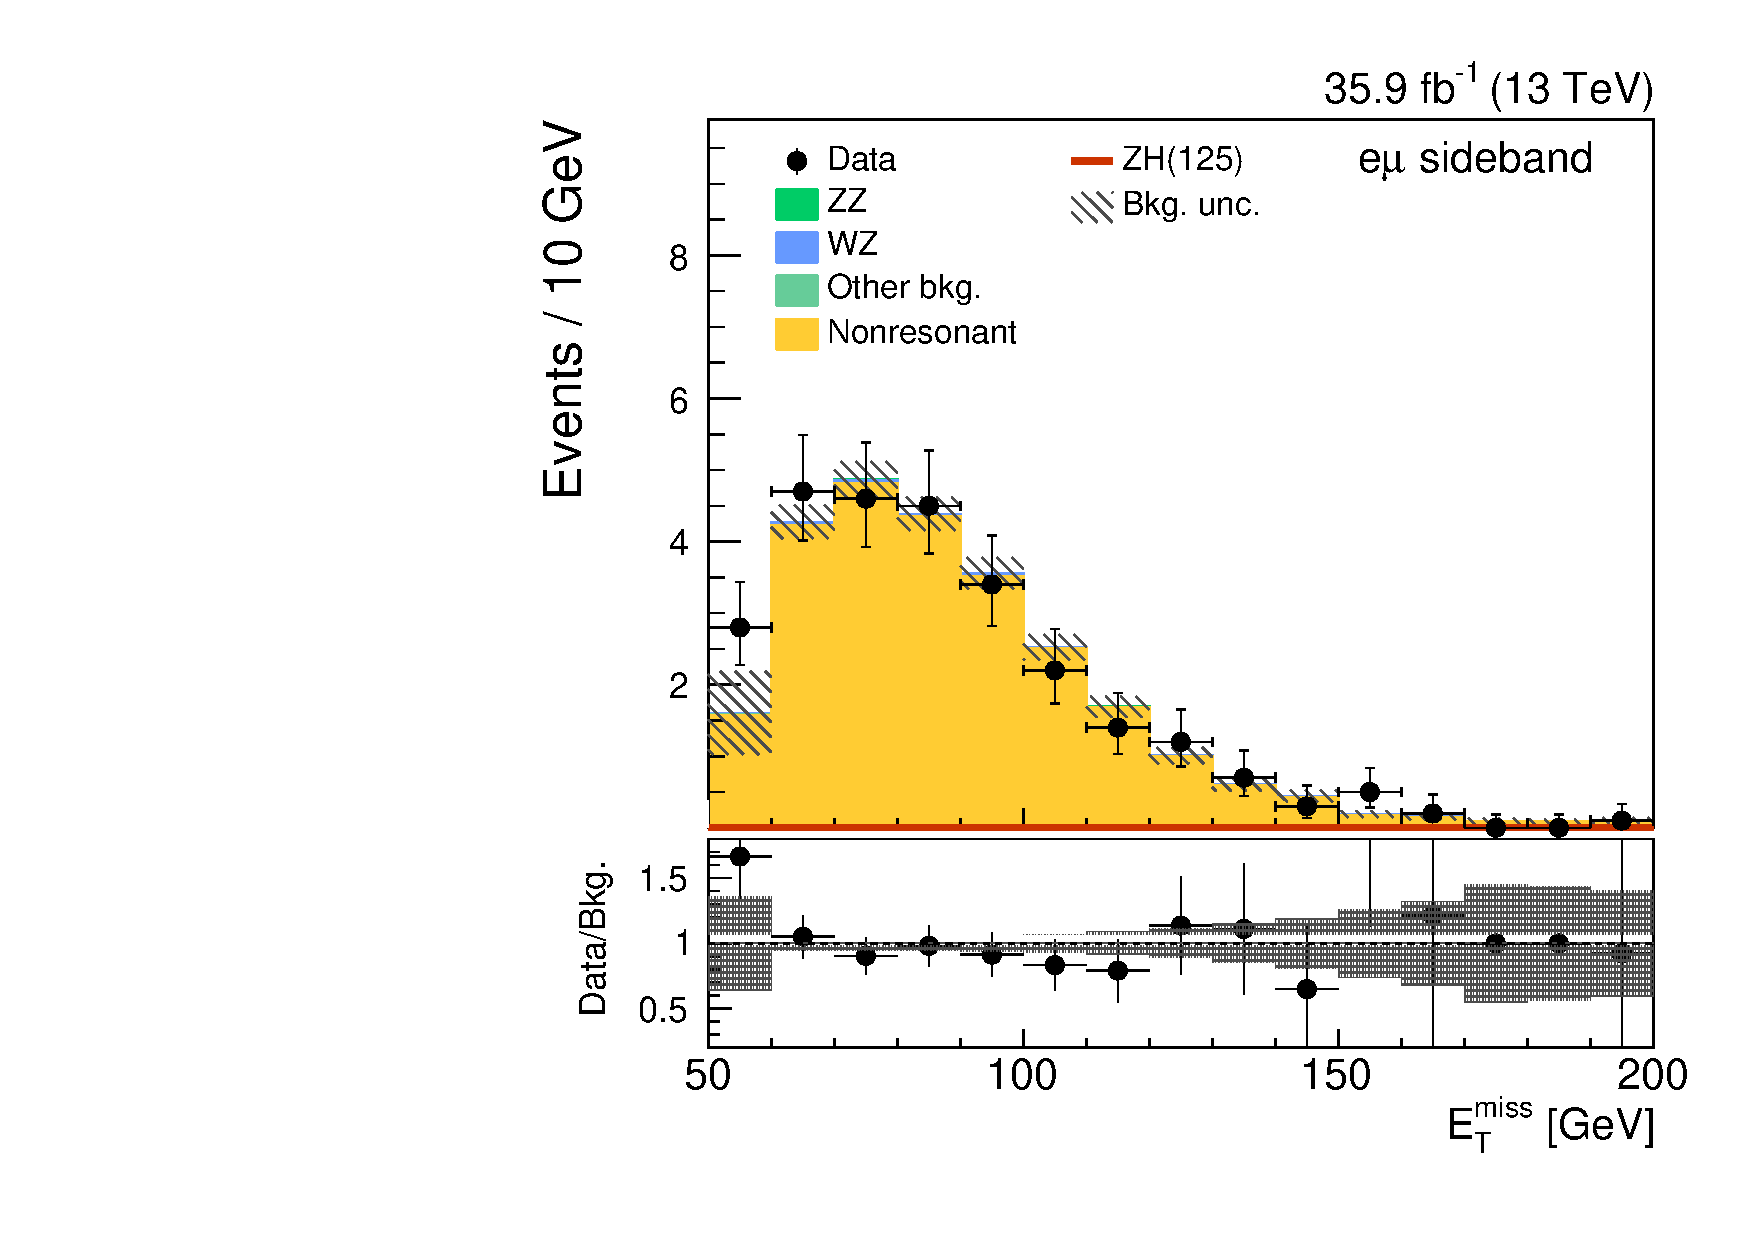
\includegraphics[width=0.46\textwidth]{figures/em_zh_1j_met_allcutsbutone.pdf}
 \end{center}
 \caption{Distributions of $|m_{e\mu}-m_{\Z}|$,
        $\Delta R_{\ell\ell}$,
        $\Delta \phi_{\ell\ell,\met}$,
        and $\met$ for $\Pe \mu$ events after applying the full selection except the variable itself.}
\label{fig:m_em}
\end{figure}

\begin{figure}[hbtp]
\centering
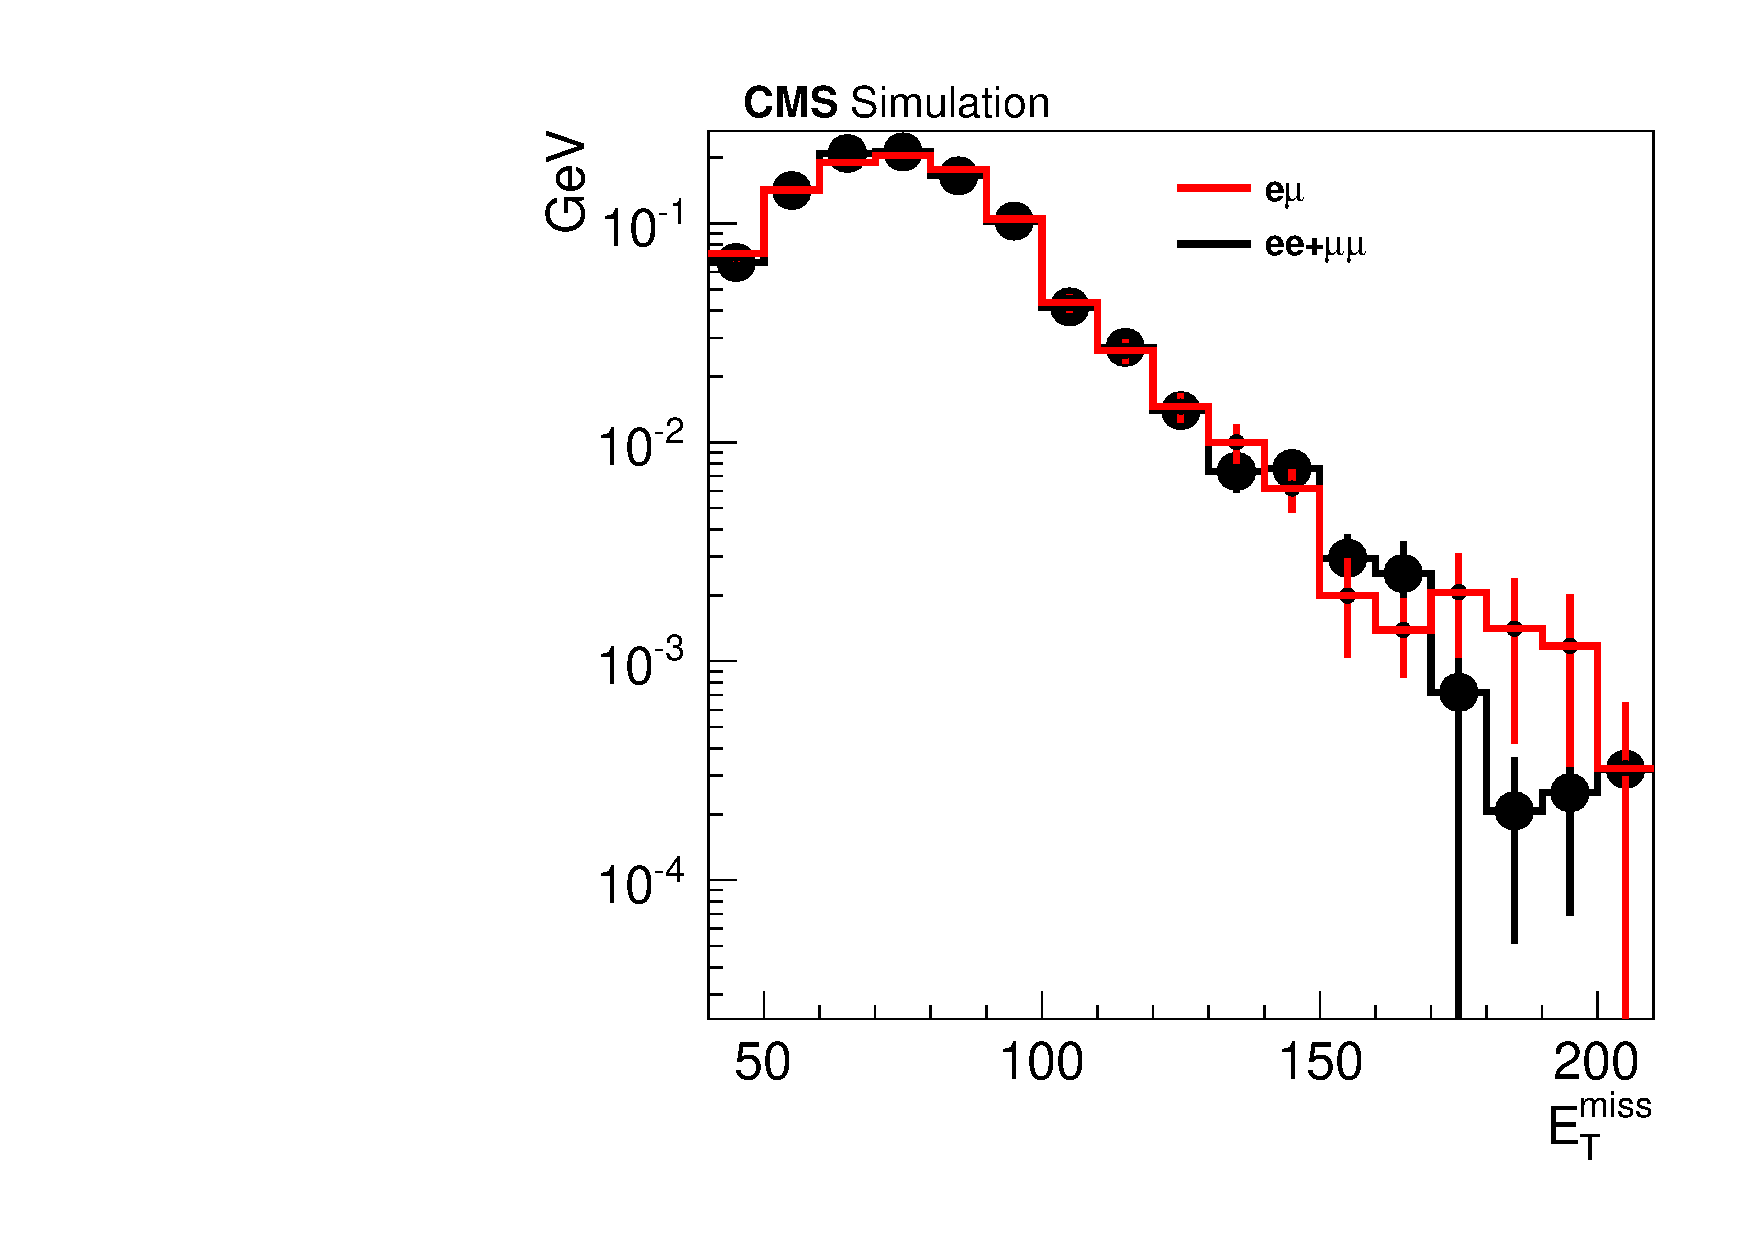
\includegraphics[width=0.48\textwidth]{figures/met_tt_ww.pdf}
\caption{Comparison of the $\met$ distributions for $\WW$+top-quark simulated 
events for $e\mu$ versus $ee+\mu\mu$ events.} 
\label{fig:met_tt_ww}
\end{figure}

\newpage
\subsection{Drell-Yan background estimation}
The Drell-Yan (DY) process is dominant in the region of low $\ETm$.
This process does not produce undetectable particles, therefore any non-zero $\ETm$ arises from
limited detector acceptance and mismeasurement.
The estimation of this background uses simulated DY events, which are normalized to data in a control region.
A scale factor is obtained by measuring the number of DY events in a $\met$ sideband of $[50, 100]\GeV$,
and is included in the maximum likelihood fit, as shown in Sec.~\ref{sec:likelihood}.

A $100\%$ uncertainty is assigned to the DY estimate in order to cover the extrapolation from the low-\met region to the higher-\met signal region.
This uncertainty has little effect on the results due to the small overall contribution from the DY process.
Extensive checks are performed to ensure that the estimation method is sensible.
By defining control regions where $\met$ mismodeling issues are expected to have a large impact, and confirming that the 
estimate from simulation for these regions still holds within the uncertainties, it is shown in Fig.~\ref{fig:met_control} that $\met$ mismodeling is under control.

For example, it is possible to calculate missing energy multiple ways and assess how well they corroborate one another.
The nominal \met quantity used in this work uses all the information from the Particle Flow reconstruction, and is called PF \met.
The so-called ``Calo \met'' is the calculation of missing energy only using the calorimeter deposits.
A large difference between the two indicates fake missing energy e.g. from mismeasurement of a jet.
The focus is how well the simulation describes the distribution in data of that disagreement, especially at high values.

Additionally, an independent estimation method using a $\gamma+\met$ control region is implemented, and the results are
confirmed to be consistent between the two methods, further increasing confidence in the approach chosen here.
%Detailed information regarding the $\gamma+\met$ studies can be found in~\cite{CMS-AN-2016-199}.

Spurious muons and mismeasured electrons were observed in the re-reconstruction of the 2016 data, due to the relaxed tracking and PF requirements of the `HIP mitigation'
described earlier in Section~\ref{ss:hips}. 
A re-analysis of the data was performed to identify and clean or correct the data for these objects.
These issues are not expected to affect our analysis in a significant manner, mainly due to our third lepton veto.
Nevertheless, the effect is negligible in our signal region. 
A correlation plot showing the effect of this cleaning is shown in Fig.~\ref{fig:met_control}.

\begin{figure}[hbtp]
  \centering
  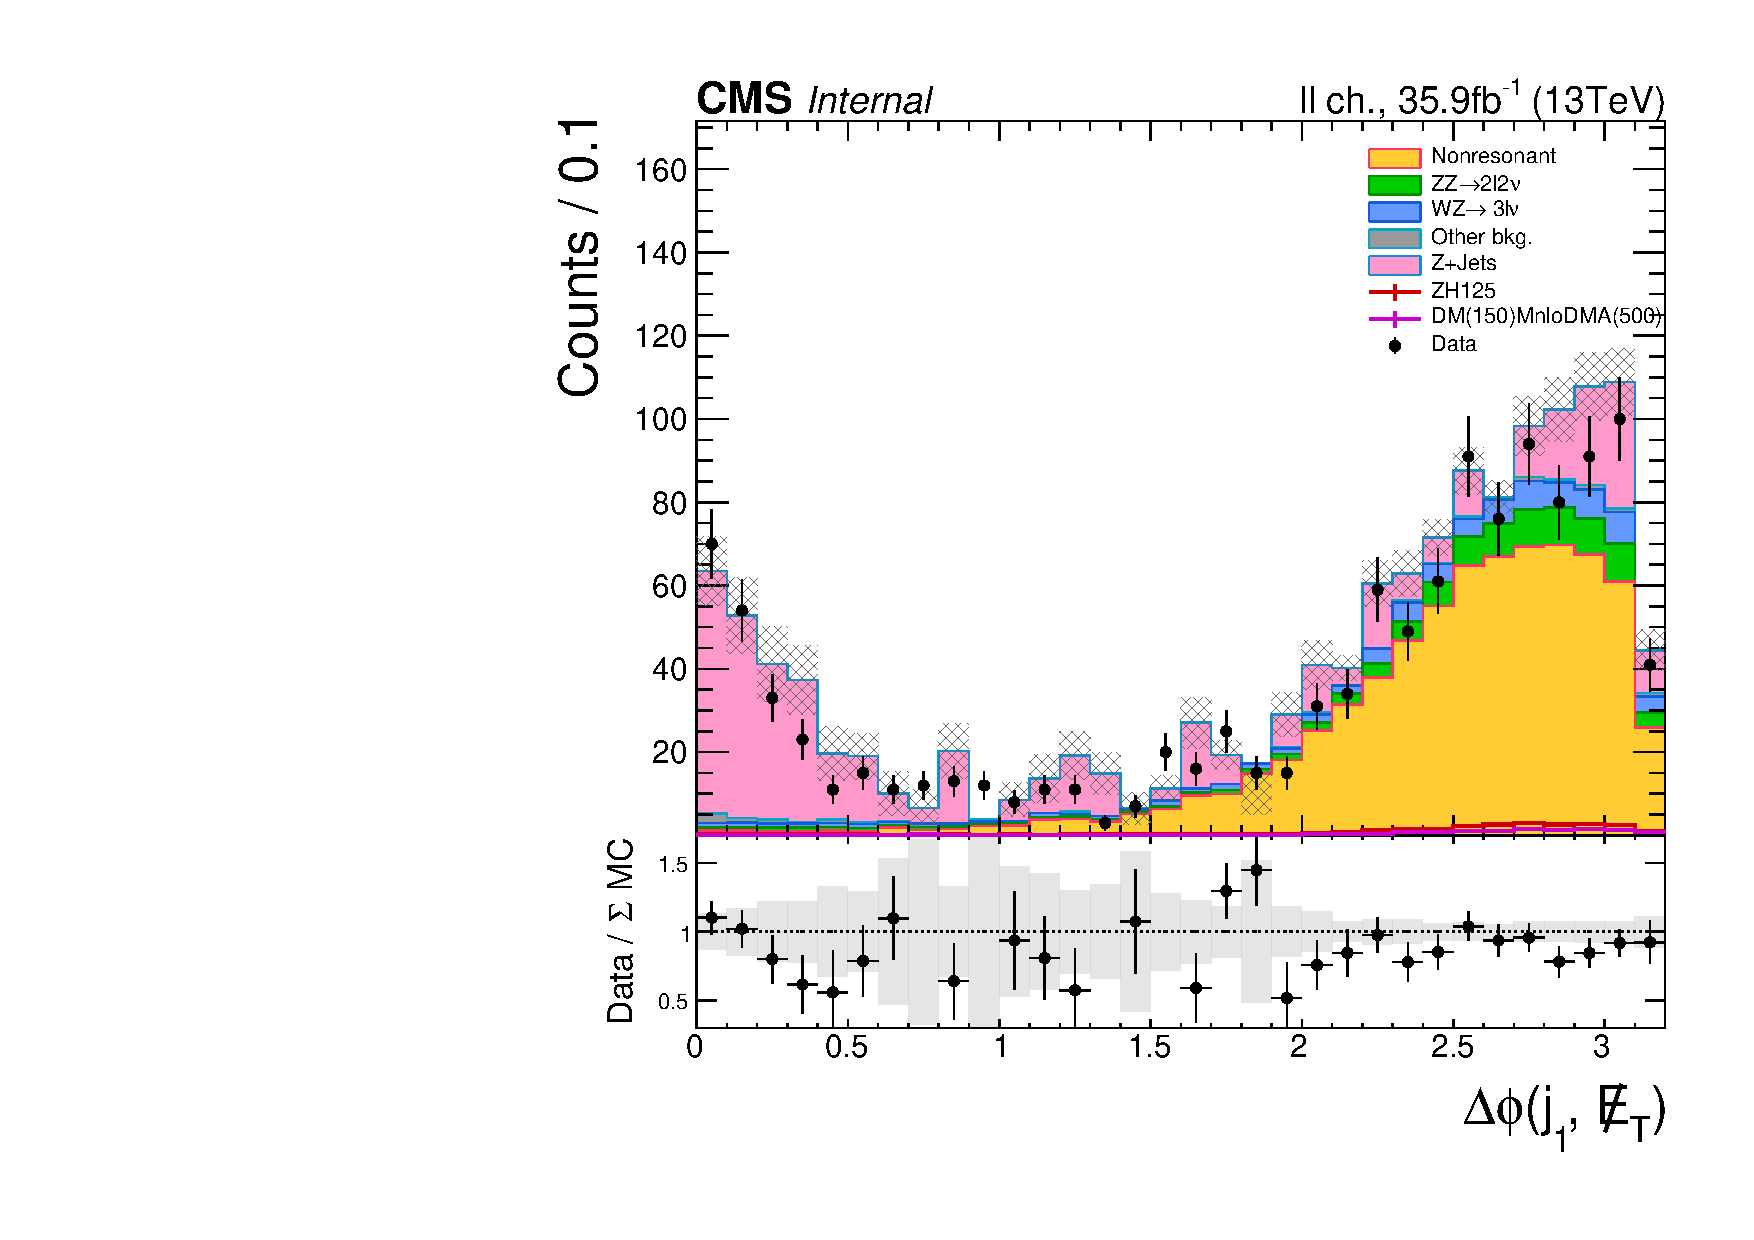
\includegraphics[width=0.48\textwidth]{figures/ll_metCheck_dPhiJetMet_failBalance.pdf}
  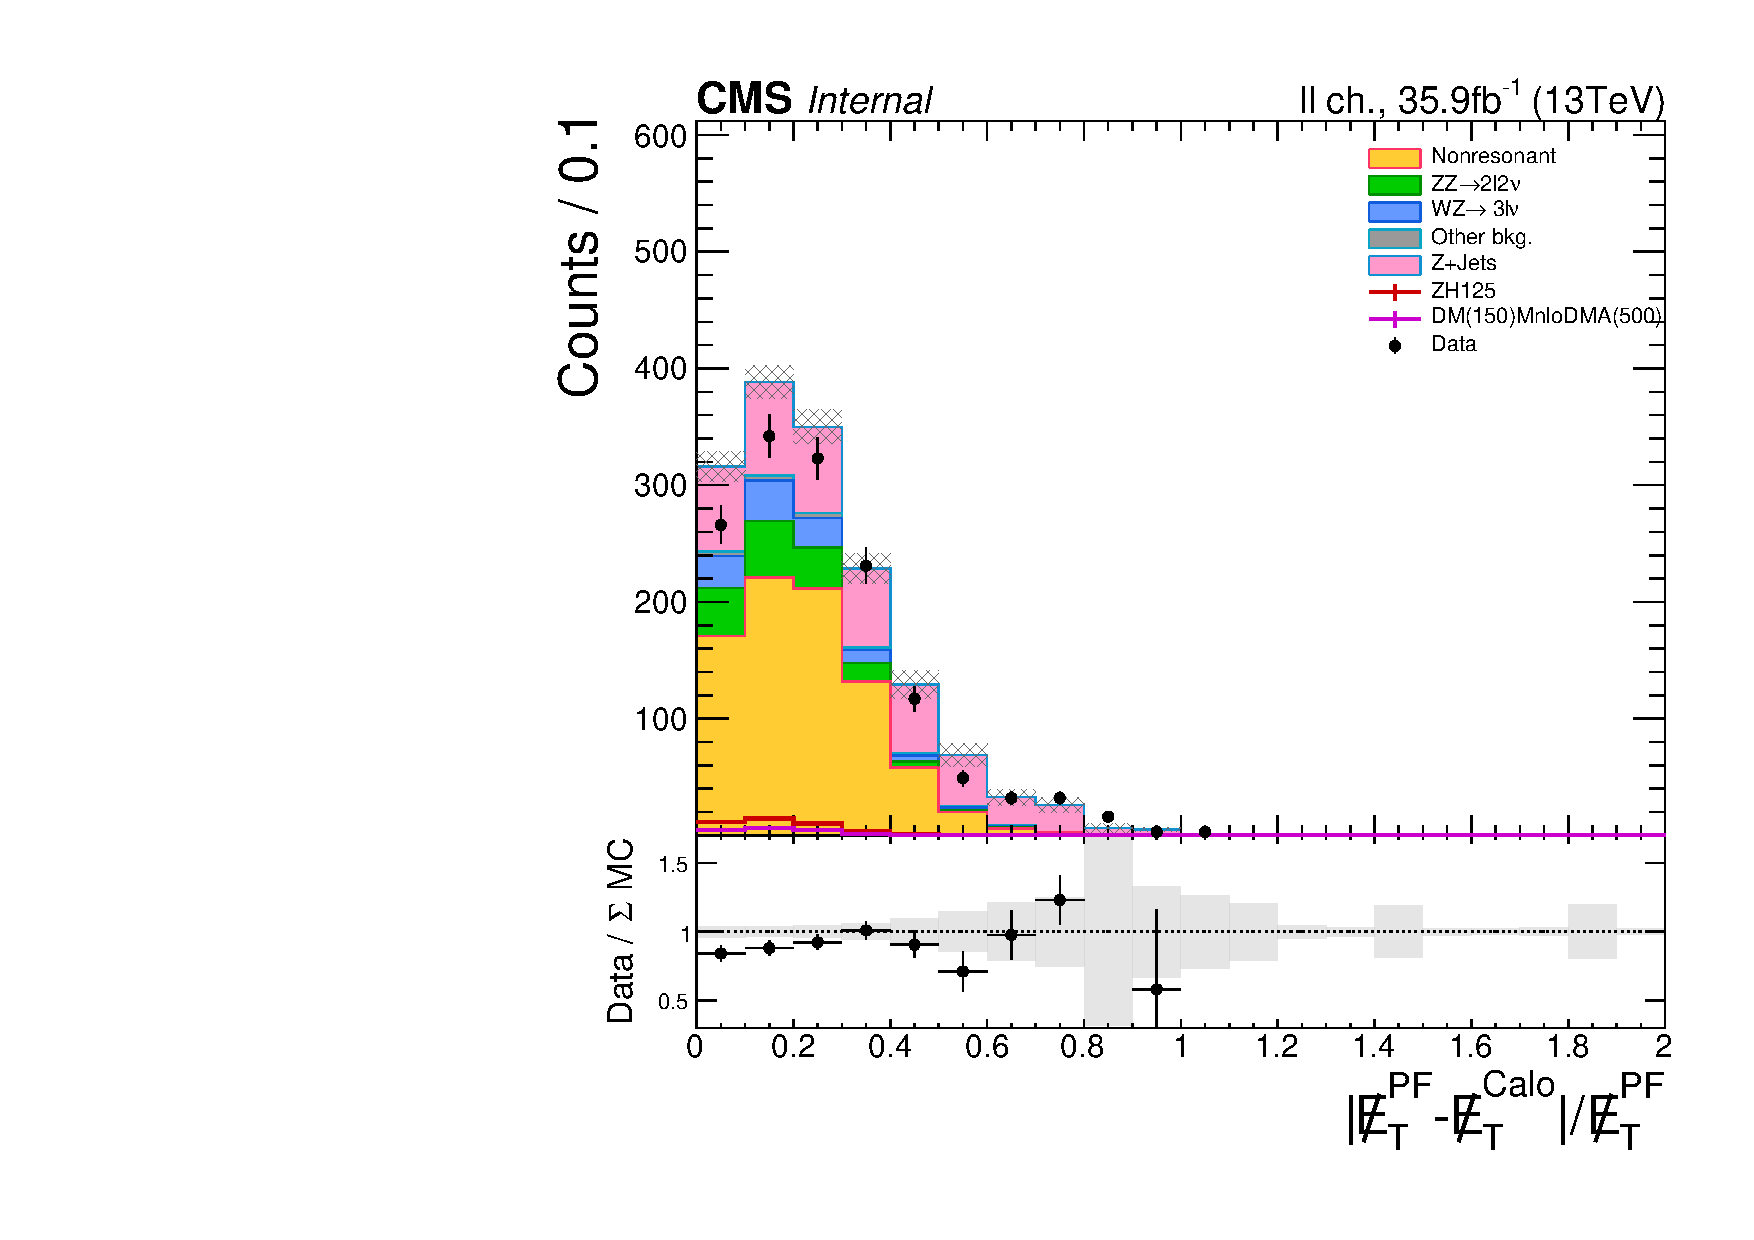
\includegraphics[width=0.48\textwidth]{figures/ll_metCheck_pfVsCaloMet_failBalance.pdf}
  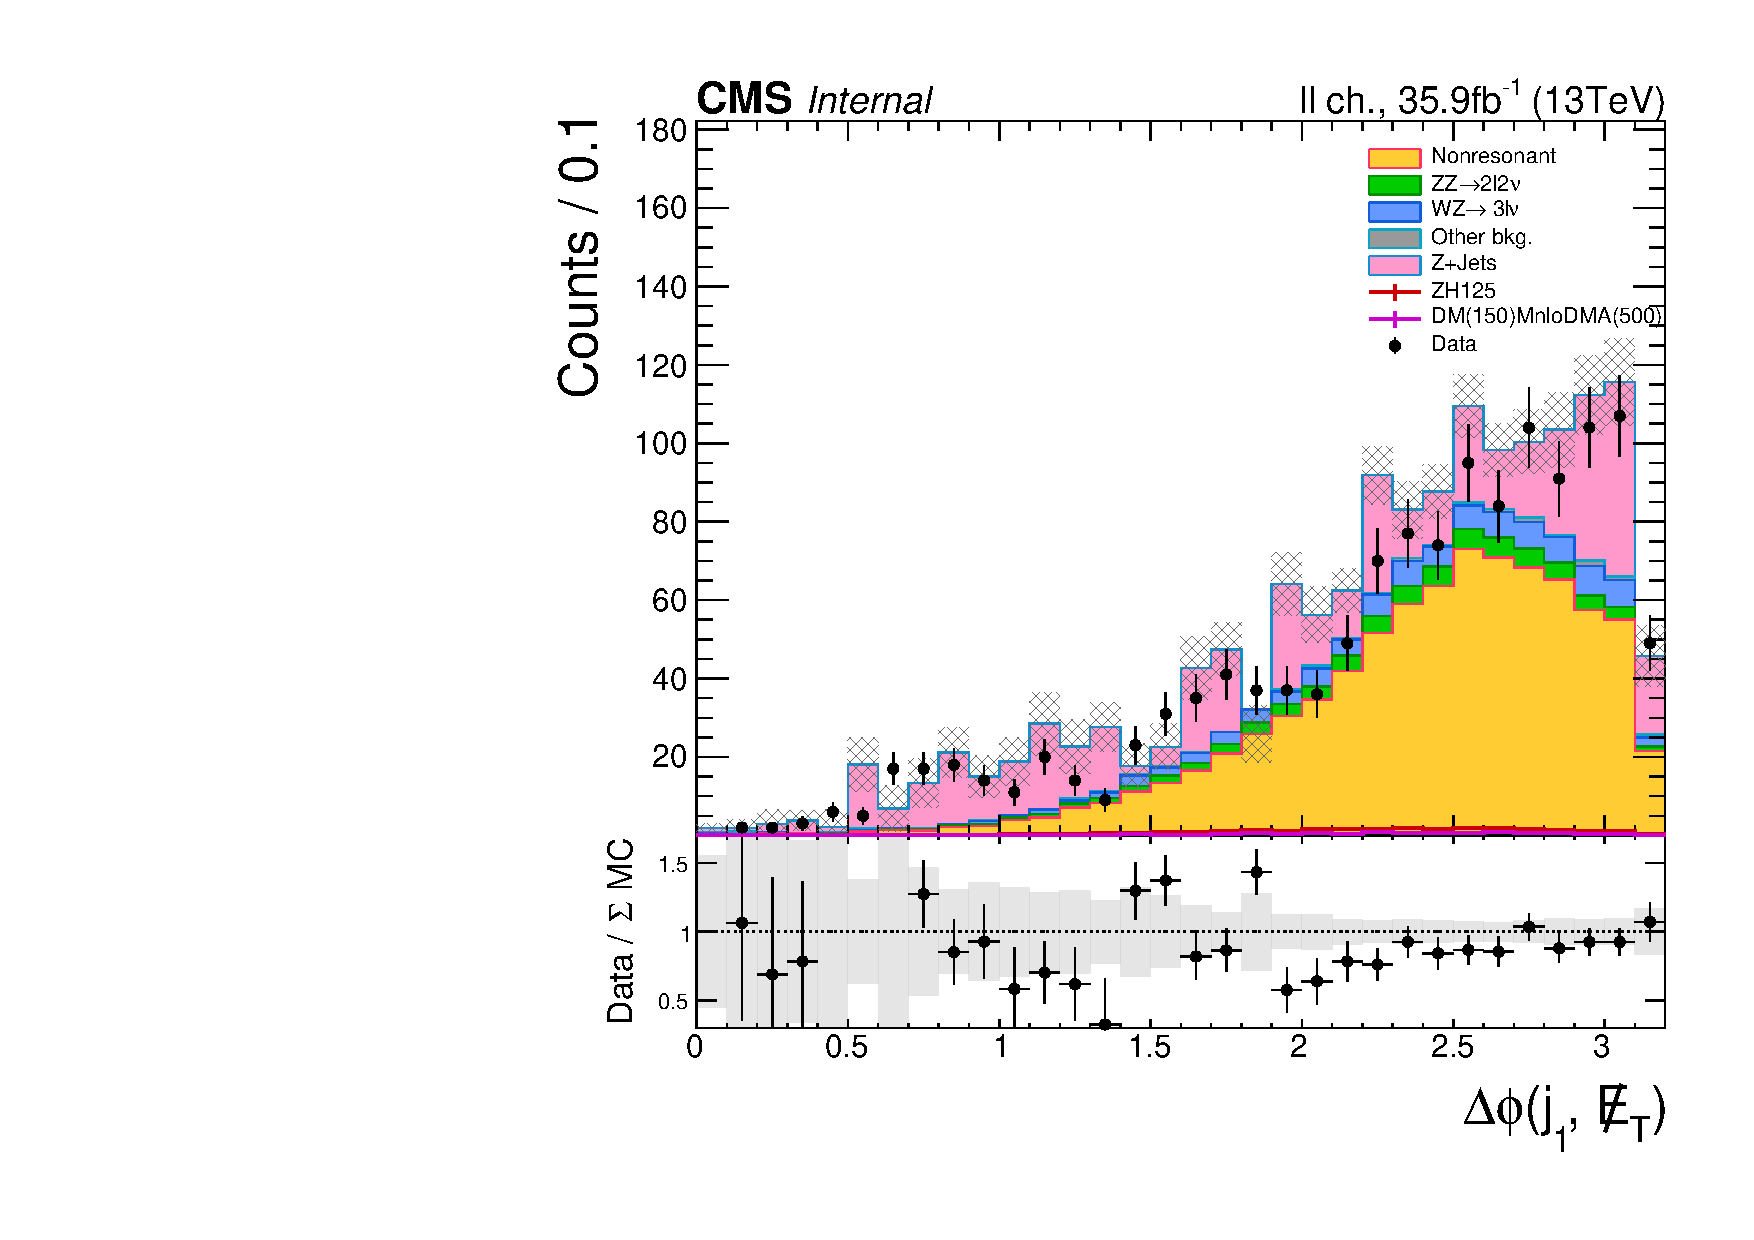
\includegraphics[width=0.48\textwidth]{figures/ll_metCheck_dPhiJetMet_failDphi.pdf}
  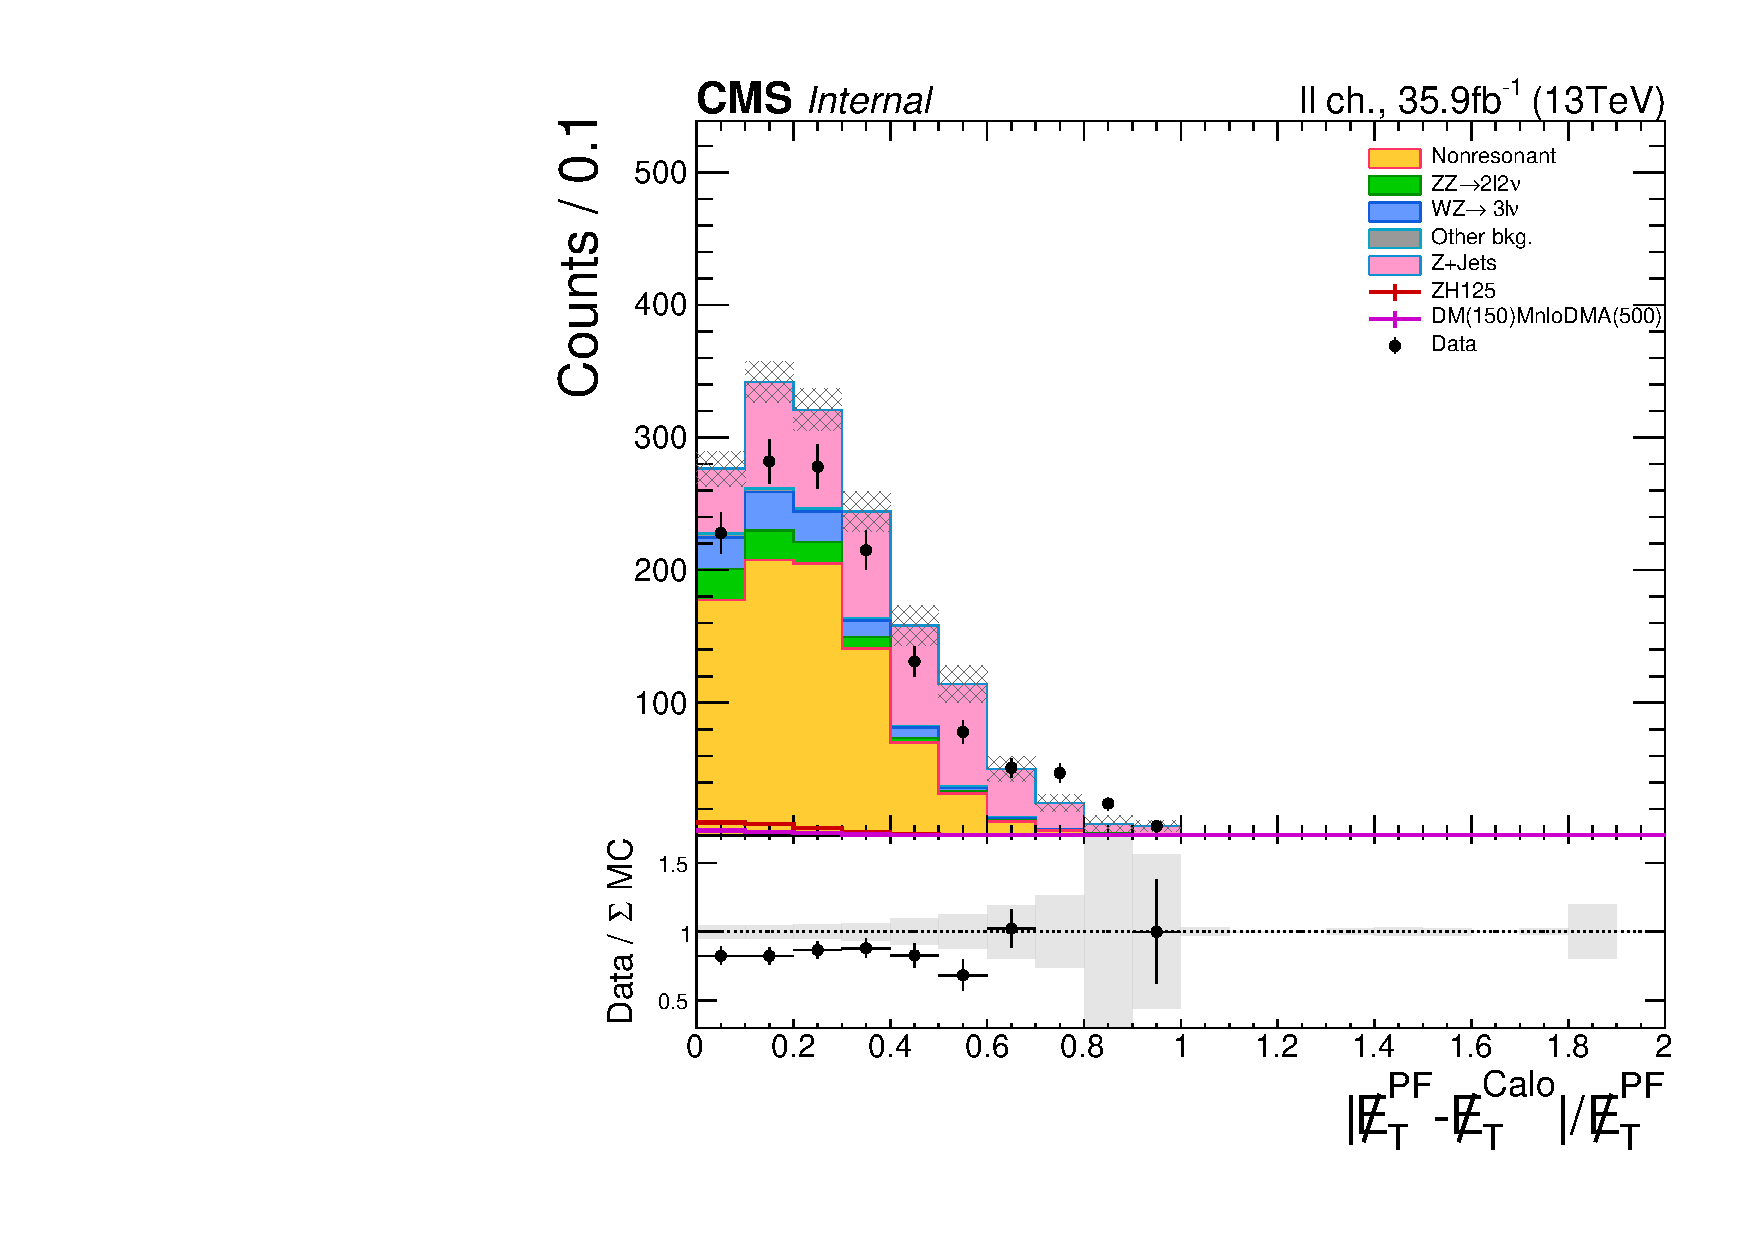
\includegraphics[width=0.48\textwidth]{figures/ll_metCheck_pfVsCaloMet_failDphi.pdf}
  \caption{
    Selection of \met mismodeling control regions, after a loose selection: $m_Z$ window, $p_{T}^{\ell\ell}>60\GeV$, $<2$ Jets, $\met>100\GeV$.
    Top row: Events failing \met Balance cut, $\Delta\phi(j,\met)$ and the PF to Calo \met ratio are plotted.
    Second row: Events failing $\Delta\phi(Z,\met)$ cut, $\Delta\phi(j,\met)$ and the PF to Calo \met ratio are plotted.
  }
  \label{fig:met_control}
\end{figure}

\begin{figure}[hbtp]
  \centering
  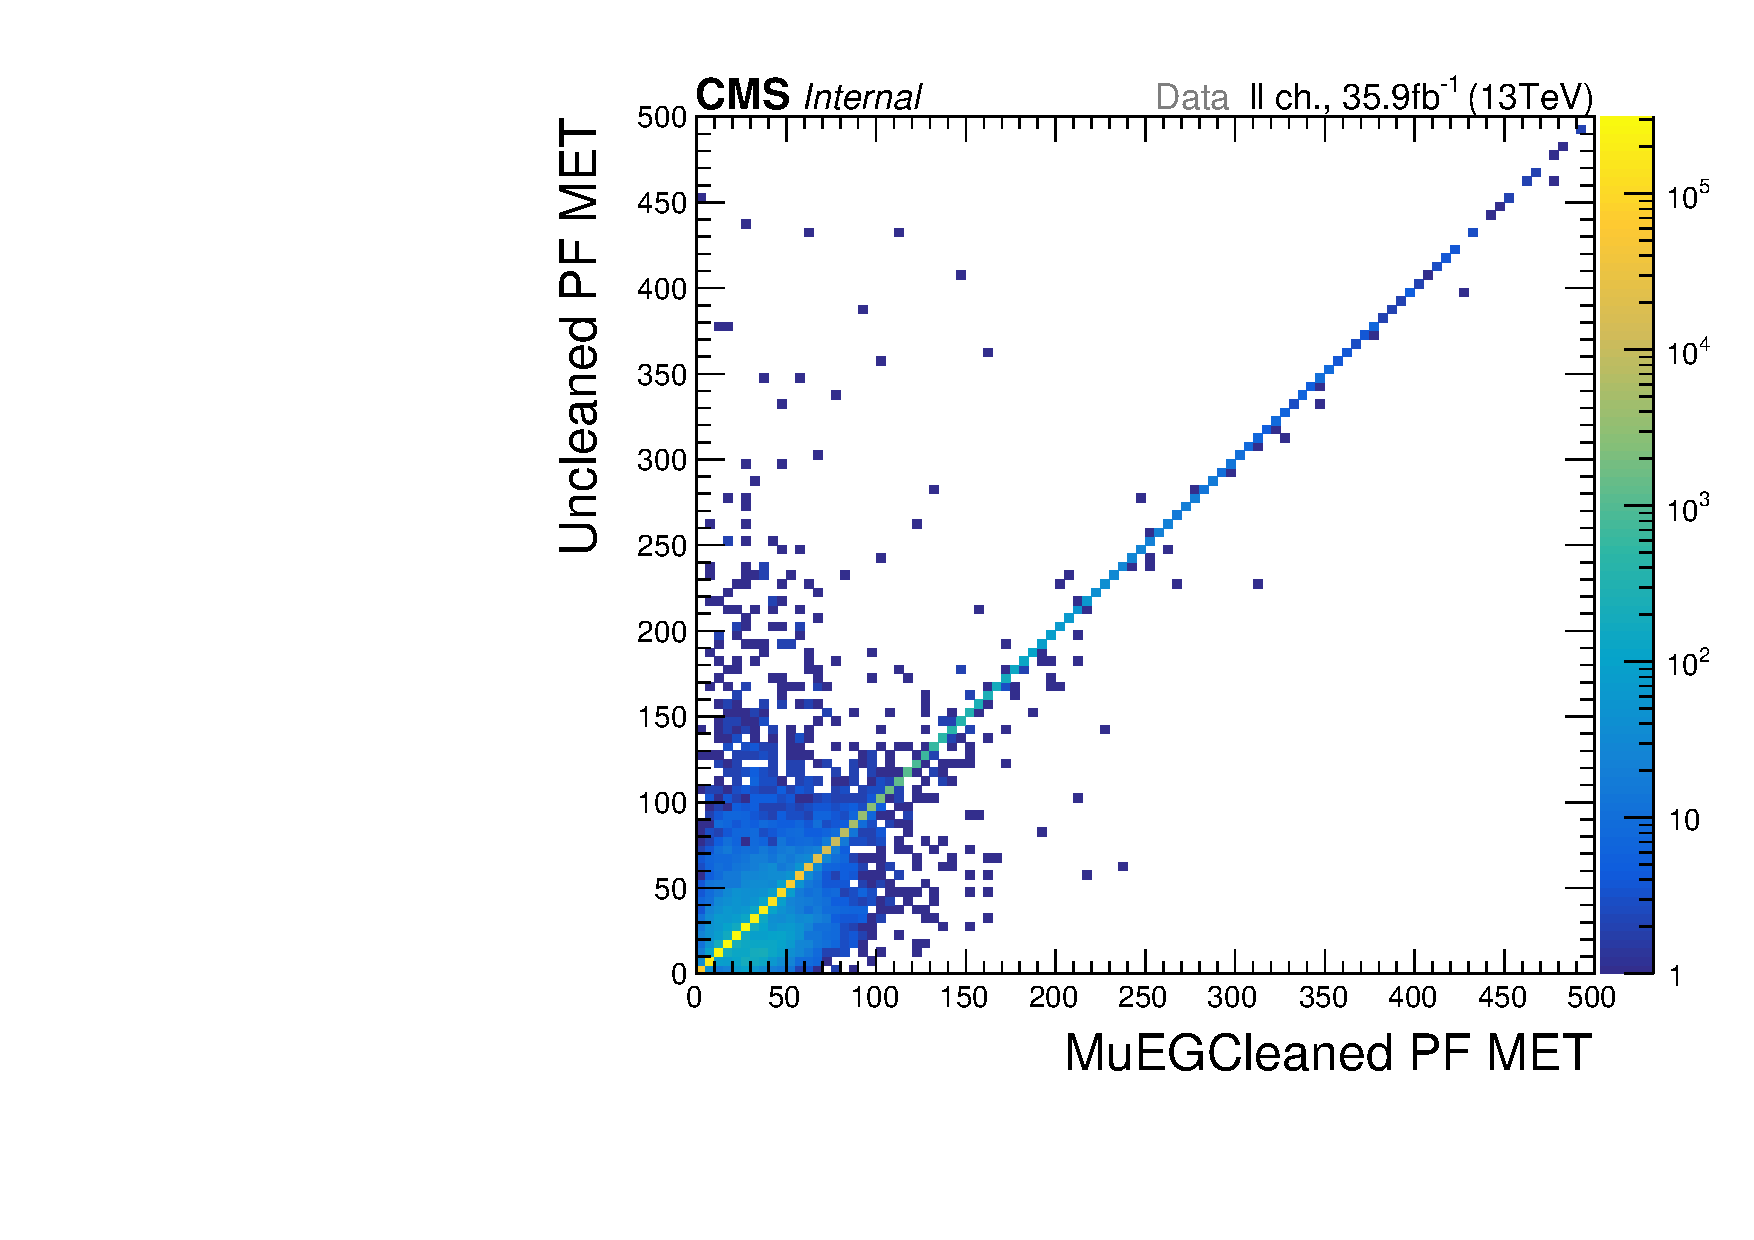
\includegraphics[width=0.48\textwidth]{figures/ll_metAltVsUncleaned.pdf}
  \caption{
    Joint disribution of the \met and the cleaned \met, showing the effect of the cleaning.
  }
  \label{fig:met_control2}
\end{figure}

\section{Systematic uncertainties}
\label{sec:dmsyst}
Systematic uncertainties in the data-based background estimates are described 
in Section~\ref{sec:dmbkg}.
Here I will list all of the uncertainties which are taken into
account in the fit to the $\met$ shapes. 
Uncertainties which do not only influence the overall normalization
(\eg the uncertainty in the luminosity measurement), but also the
distribution of relevant kinematic observables (\eg the uncertainty in
the jet energy scale), are treated as shape uncertainties. Their
impact is evaluated by performing the full analysis not only for the
central value of the relevant parameter, but also with its value
shifted up and down by one standard deviation. The final varied
$\met$-distributions are used as input for the limit calculation. For
each source of uncertainty, the impact in different bins of the
$\met$-distribution is thus considered fully correlated, while
independent sources of uncertainty are treated as uncorrelated. 

%%%%%%%%%%%%%%%%%%%%%%%%%%%%%%%%%%
\subsection{Luminosity}
%%%%%%%%%%%%%%%%%%%%%%%%%%%%%%%%%%

The assigned uncertainty to the integrated luminosity measurement for
the data set used in this analysis is 2.5\%~\cite{CMS:2017sdi}.

%%%%%%%%%%%%%%%%%%%%%%%%%%%%%%%%%%
\subsection{Trigger, lepton reconstruction and identification efficiencies}
%%%%%%%%%%%%%%%%%%%%%%%%%%%%%%%%%%
Discrepancies in the lepton reconstruction and identification
efficiencies between data and simulation are corrected by applying
to all MC samples data-to-simulation scale factors measured using $\dyll$ 
events in the $\cPZ$ peak region~\cite{wzxs} that are recorded with unbiased triggers. 
These factors depend on the lepton $\pt$ and $\eta$ and are within a few percent for electrons and muons.
The uncertainty in the determination of the trigger efficiency leads to an uncertainty 
smaller than 1\% in the expected signal yield. Residual difference between the analysis 
lepton requirements with respect to the trigger selections is well covered by 
the uncertainty in the trigger efficiency. 

%%%%%%%%%%%%%%%%%%%%%%%%%%%%%%%%%%
\subsection{Lepton momentum and electron energy scale}
%%%%%%%%%%%%%%%%%%%%%%%%%%%%%%%%%%

The lepton momentum scale uncertainty is computed by varying the
momentum of the leptons by their uncertainties. 
The uncertainty on the muon and electron transverse momenta is assumed to be 1\%.

%%%%%%%%%%%%%%%%%%%%%%%%%%%%%%%%%%
\subsection{Jet energy scale (JES) and resolution (JER)}
%%%%%%%%%%%%%%%%%%%%%%%%%%%%%%%%%%

The uncertainty in the calibration of the jet energy scale and resolution
directly affects the acceptance of the requirement $< 2$~jets, 
the \ETm computation, and all the cuts related to jets. 

The estimate of the jet energy scale uncertainty is performed varying the jet energy scale up and down by 1$\sigma$.
The variation corresponds to a simple re-scaling of the jet four-momentum as
$P\rightarrow P \cdot (1 \pm \delta\pt^{JES}/{\pt})$, where 
$\delta\pt^{JES}$ is the absolute uncertainty on the jet energy scale
which is parametrized as function of the $\pt$ and $\eta$ of the jet. 
For more details on the jet energy scale prescription, see Ref.~\cite{JES2011}. 

In order to account for the systematic uncertainty of the jet resolution smearing procedure,
the resolution scale factors are varied up and down within their uncertainty.

%%%%%%%%%%%%%%%%%%%%%%%%%%%%%%%%%%
\subsection{B-tagging efficiency}
%%%%%%%%%%%%%%%%%%%%%%%%%%%%%%%%%%

In this analysis, b-tagging is used to reject events with real b-jets in 
the final state since the signal events have little b-jet content. 
For numerous reasons, the b-tagging efficiency of light flavor, c-quark, and b-quark jets varies between data and simulation.
To account for this, a recommendation provided by the collaboration's B-Tagging and Vertexing Group is used to reweight the b-tagging (in)efficiencies of the selected jets~\cite{Sirunyan:2017ezt}.

The b-tagging efficiency determination relies on a data sample of jets enriched in heavy flavor content.
This is obtained by requiring a primary AK4 jet containing a soft muon, along with a secondary "away-jet" having separation $\Delta R>1.5$ with respect to the first jet.
Fit templates for the different jet flavors are built from muon-enriched simulated samples of QCD processes.
Various systematic uncertainties are considered for this method:
\begin{itemize}
\item Relative contribution of gluon splitting 
\item Modelling of b-quark fragmentation
\item Relative contribution of light jets and c-quark jets
\item Pileup
\item Muon selection
\item Away-jet selection
\item Jet energy scale
\end{itemize}

The impact of these systematic uncertainties on the sensitivity of this analysis is only 0.1\%.

%%%%%%%%%%%%%%%%%%%%%%%%%%%%%%%%%%
\subsection{Pileup}
%%%%%%%%%%%%%%%%%%%%%%%%%%%%%%%%%%

As discussed in Sec.~\ref{subsec:puweights}, MC samples are re-weighted to
reproduce the pileup conditions observed in data.
To compute the uncertainty related to this re-weighting procedure, the pileup distribution is 
computed not only for the nominal value of the minimum bias cross-section,
but also for $\pm5\%$ variations of it.
The resulting variations in weights are propagated through the analysis chain, 
and the varied \met spectra are used to as input to the maximum likelihood fit.
The variation of the final yields induced by this procedure is less than 1\% in MC-estimated processes.


%%%%%%%%%%%%%%%%%%%%%%%%%%%%%%%%%%
\subsection{Theoretical uncertainties}
\label{subsec:dmtheo}
%%%%%%%%%%%%%%%%%%%%%%%%%%%%%%%%%%

Uncertainties on the normalization for $\Z\Z$, $\W\Z$ and signal
processes are derived from variations of the QCD scale, $\alpha_{s}$
and parton distribution functions (PDFs)
variations~\cite{Botje:2011sn,Alekhin:2011sk,Lai:2010vv,Martin:2009iq,Ball:2011mu,MCFM}. 

The PDF and $\alpha_s$ uncertainties for signal and background processes are estimated 
from the standard deviation of weights from the replicas provided in the 
NNPDF3.0 parton distribution set~\cite{nnpdf}.

The samples for the signals and leading backgrounds were generated at NLO in QCD,
and the scale uncertainties are estimated using the weights
stored in the respective samples. For the ZZ process, this procedure is rather conservative
in the sense that the prediction is corrected to NNLO in QCD, but the assumed uncertainty reflects
the precision of the NLO generator.

The PDF uncertainties for the PDF4LHC PDF sets are assessed in the following way.
The final distribution for the variable of interest is reweighted bin-by-bin using the PDF4LHC PDF sets.
This produces $1+N_{\textrm{mem}}$ distributions, where $N_{\textrm{mem}}$ is the number of alternative PDF sets used.
The uncertainty $\delta^{\textrm{PDF}}\sigma$ on the cross section $\sigma$ is calculated in a bin-by-bin approach via
%%%%%%%%%%%%%%%%%%
\begin{equation}
\delta^{\textrm{PDF}} \sigma= \sqrt{ \frac{1}{N_{\textrm{mem}} - 1} \sum_{k=1}^{N_{\textrm{mem}}} \left(\sigma^{(k)} - \langle \sigma \rangle\right)^2 }\,,
\end{equation}
%%%%%%%%%%%%%%%%%%
whereby the mean value of the cross section $\sigma$ is given by
%%%%%%%%%%%%%%%%%%
\begin{equation}
\langle\sigma\rangle = \frac{1}{N_{\textrm{mem}}} \sum_{k=1}^{N_{\textrm{mem}}} \sigma^{(k)},
\end{equation}
%%%%%%%%%%%%%%%%%%

Now, let us return to the discussion of diboson theory introduced in Chapter~\ref{chap:dibosons}, Section~\ref{sec:vvtheo}.
The uncertainties from the higher order theoretical calculations are propagated to the \ETm distribution.
The NLO electroweak and NNLO QCD corrections each carry a ``shape uncertainty,''
meaning the corresponding nuisance parameters in each bin of \ETm are fully correlated for the
purposes of the maximum likelihood fit.

%%%%%%%%%%%%%%%%%%%%%%%%%%%%%%%%%%
\subsection{MC statistical uncertainty}
%%%%%%%%%%%%%%%%%%%%%%%%%%%%%%%%%%

All background estimation procedures in this analysis rely on some degree
of simulation shape information.
For the DY and NRB processes, the final shape is taken directly from simulation, 
while the WZ and ZZ estimates only depend on the ratio of the MC expectations for the processes.
In any case, the limited number of simulated events gives rise to a statistical uncertainty.
This uncertainty is treated as fully uncorrelated for each process classification and distribution bin.
%%%%%%%%%%%%%%%%%%%%%%%%%%%%%%%%%%
\subsection{Summary}
\label{sec:syst_summary}
%%%%%%%%%%%%%%%%%%%%%%%%%%%%%%%%%%

The summary of all systematic uncertainties and their correlations is shown in Table~\ref{tab:syst}.
The following uncertainties are considered for the shape variation:
\begin{itemize}
\item lepton efficiencies and momentum resolution 
\item missing transverse energy 
\item jet energy scale and resolution 
\item b-tagging efficiency 
\item pileup reweighting 
\item limited number of Monte Carlo events
\item missing mixed QCD-EW corrections
\item missing QCD higher-order corrections
\item PDF
\end{itemize}

The overall signal efficiency uncertainty is estimated to be about 11\%
and is dominated by the theoretical uncertainty due to missing
higher-order corrections and PDF uncertainties. The total uncertainty in the 
background estimations in the signal region is about 10\%, which is 
dominated by the theoretical uncertainties in the ZZ and WZ processes.

The post-fit pulls and the impacts of the top 30 uncertainties, ordered by decreasing importance,
are shown in Figure~\ref{fig:impacts}.

\begin{table}[htb]
\caption{
Summary of systematic uncertainties.
Each uncertainty represents the variation of the relative yields of the processes in the signal region.
A particular uncertainty is fully correlated across processes for which it contributes, including those processes which are also present in control regions.
The symbol ``-'' indicates that the systematic uncertainty does not contribute or is deemed negligible.
For shape uncertainties (indicated with a *), the numbers correspond to the overall effect of the shape variation on yield or acceptance.
The impact on the expected limit, i.e. the relative decrease in the median expected upper limit on signal strength upon removing the nuisance, is also evaluated with respect to the SM Higgs signal.
\label{tab:syst}
} 
\centering
{\scriptsize
\setlength{\tabcolsep}{3pt} % Default value: 6pt
\begin{tabular}{lccccccc}
\hline
\multirow{2}{*}{Source of uncertainty}         & \multicolumn{6}{c}{Effect (\%)}                                              & Impact on   \\
                                               & Signal     & ZZ         & WZ         & NRB         & DY         & Other      & exp. limit  \\
\hline
* VV Electroweak Corrections                   & -          & 10         & -4         & -           & -          & -          & 14 \%      \\
* QCD Scale, VV backgrounds                    & -          & 9          & 4          & -           & -          & -          & \multirow{8}{*}{2 \%} \\
* QCD Scale, Higgs Signal                      & 3.5        & -          & -          & -           & -          & -          &            \\
* QCD Scale, Dark Matter Signal                & 5          & -          & -          & -           & -          & -          &            \\
* PDF, WZ background                           & -          & -          & 1.5        & -           & -          & -          &            \\
* PDF, ZZ background                           & -          & 1.5        & -          & -           & -          & -          &            \\
* PDF, Higgs Signal                            & 1.5        & -          & -          & -           & -          & -          &            \\
* PDF, Dark Matter Signal                      & 1-2        & -          & -          & -           & -          & -          &            \\
\hline
* MC Statistics, Nonresonant                   & -          & -          & -          & 5           & -          & -          & \multirow{5}{*}{1 \%}  \\
* MC Statistics, Drell-Yan                     & -          & -          & -          & -           & 30         & -          &            \\
* MC Statistics, ZZ                            & -          & 0.1        & -          & -           & -          & -          &            \\
* MC Statistics, WZ                            & -          & -          & 2          & -           & -          & -          &            \\
* MC Statistics, Higgs Signal                  & 1          & -          & -          & -           & -          & -          &            \\
* MC Statistics, DmSimp Signals                & 3          & -          & -          & -           & -          & -          & -          \\
\hline
NRB extrapolation to signal region             & -          & -          & -          & 20          & -          & -          & $<1$ \%       \\
Drell-Yan extrapolation to signal region       & -          & -          & -          & -           & 100        & -          & $<1$ \%       \\
Non-prompt backgrounds (signal region)         & -          & -          & 3          & -           & -          & -          & $<1$ \%       \\
Non-prompt backgrounds (WZ control region)     & -          & -          & -          & -           & 30         & -          & $<1$ \%       \\
\hline                                                                                                                              
Luminosity                                     & \multicolumn{6}{c}{2.6}                                                      & $<1$ \%        \\
\hline
* Electron Efficiency                          & \multicolumn{6}{c}{1.5}                                                      & \multirow{9}{*}{1 \%}  \\
* Muon Efficiency                              & \multicolumn{6}{c}{1}                                                        &           \\
* Electron energy scale                        & \multicolumn{6}{c}{1-2}                                                      &           \\
* Muon energy scale                            & \multicolumn{6}{c}{1-2}                                                      &           \\
* Jet Energy Scale                             & \multicolumn{6}{c}{1-3 (typically anti-correlated with yield)}               &           \\
* Jet Energy Resolution                        & \multicolumn{6}{c}{1 (typ. anti-correlated)}                                 &           \\
* Unclustered Energy Scale (MET)               & \multicolumn{6}{c}{1-4 (typ. anti-correlated), strong in DY}                 &           \\
* Pileup                                       & \multicolumn{6}{c}{1 (typ. anti-correlated)}                                 &           \\
* B-tagging fake efficiency                    & \multicolumn{6}{c}{0.1}                                                      &           \\
\hline
\end{tabular}
}
\end{table}

\begin{figure}[hbtp]
 \begin{center}
   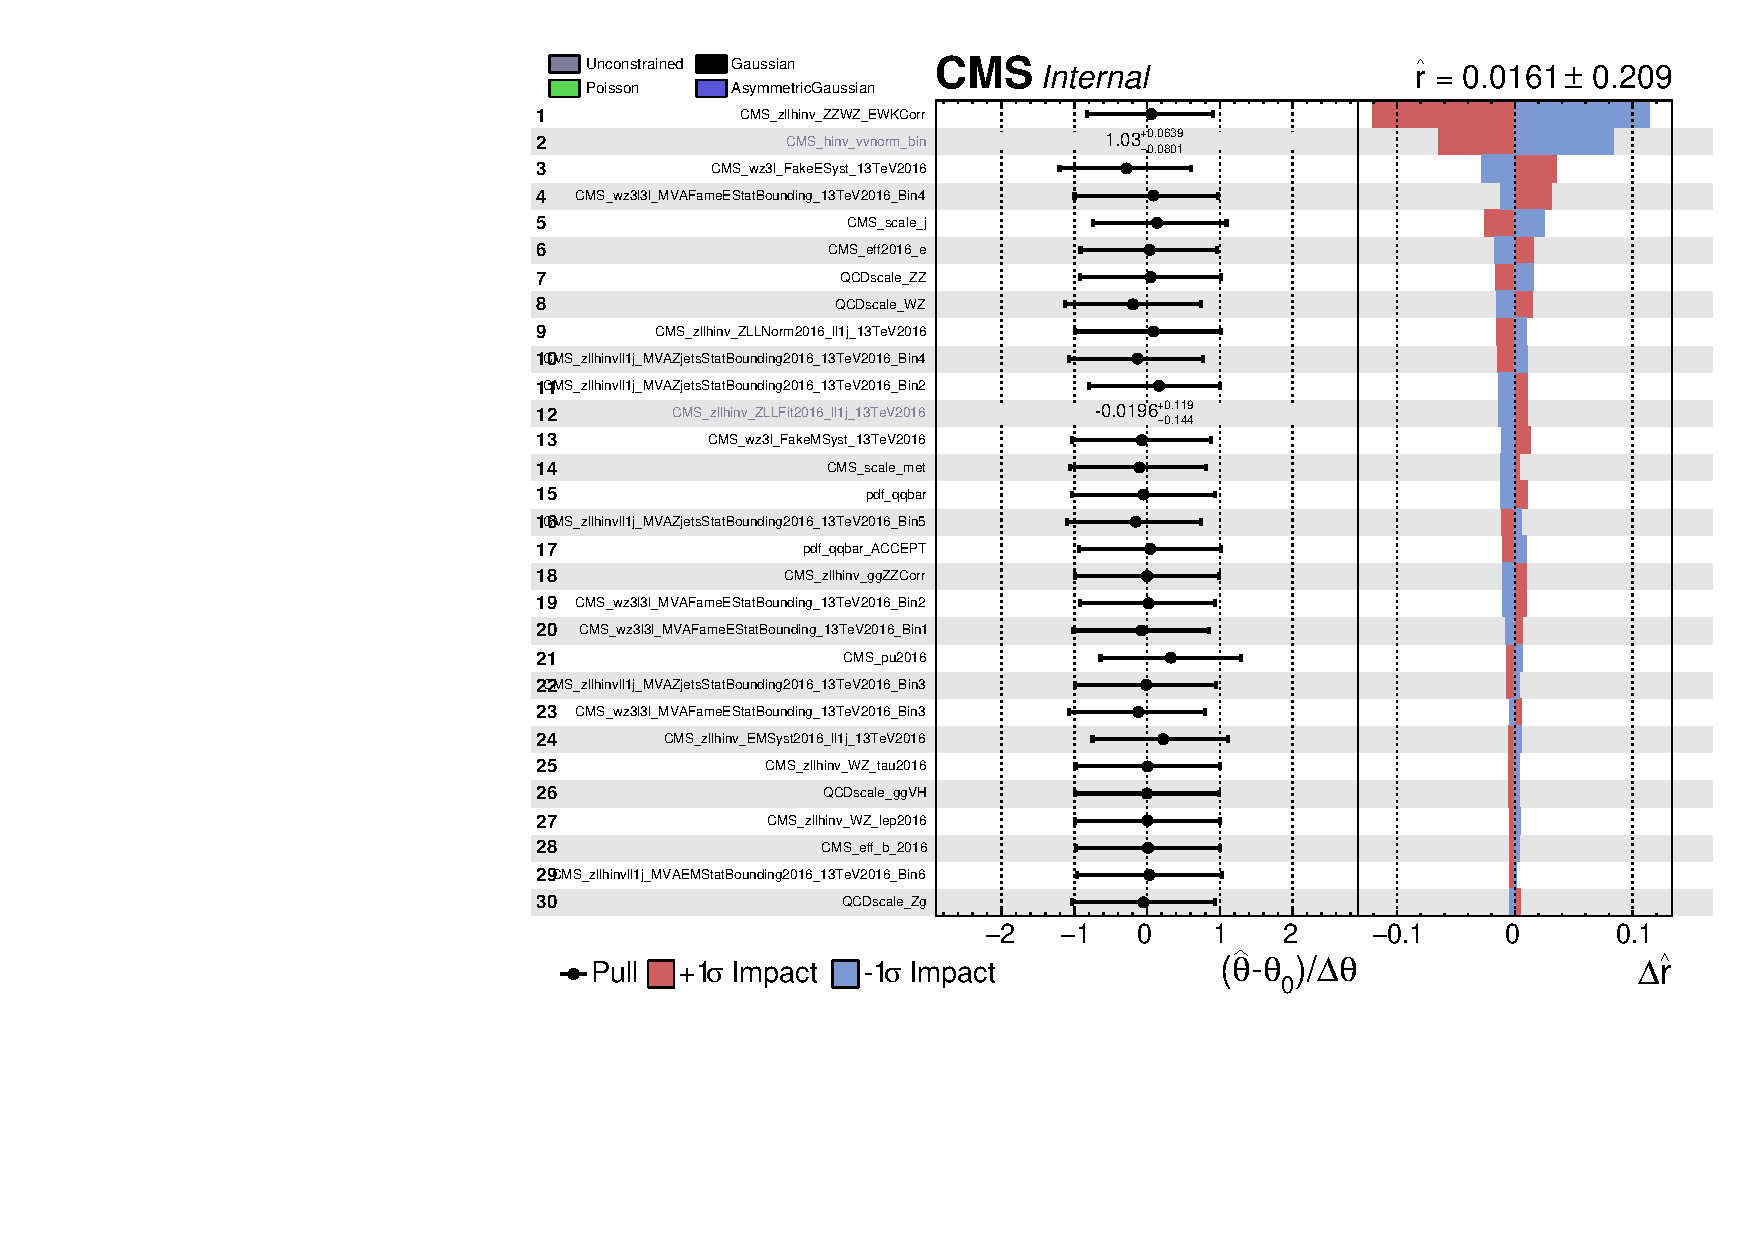
\includegraphics[width=0.92\textwidth,page=1]{figures/impacts_zmet_da.pdf}
 \end{center}
 \caption{Top uncertainties at $\usedLumi$ for a 125 $\GeV$ scalar boson mediator, ranked by decreasing importance. The codenames are explained as follows:
\texttt{CMS\_zllhinv\_ZZWZ\_EWKCorr} is the diboson electroweak uncertainties.
\texttt{CMS\_hinv\_vvnorm\_bin} is the ZZ/WZ ratio parameter from Section~\ref{sec:likelihood}. 
\texttt{CMS\_wz3l\_FakeESyst\_13TeV2016} is the uncertainty on MC simulation for producing an electron fake to give 3 leptons in the 3-lepton control sample.
\texttt{CMS\_wz3l3l\_MVAFameEStatBounding\_13TeV2016\_Bin4} is a statistical nuisance on a bin of this electron fake process.
\texttt{CMS\_scale\_j} is the jet energy scale uncertainty.
\texttt{CMS\_eff2016\_e} is the uncertainty on the electron identification efficiency.
\texttt{QCDscale\_ZZ} is the effect of the QCD scale on the ZZ process.
\texttt{QCDscale\_WZ} is the effect of the QCD scale on the WZ process.
\texttt{CMS\_zllhinv\_ZLLNorm2016\_ll1j\_13TeV2016} is the effect of the 100\% uncertainty on the Drell-Yan + fake \met process extrapolating from the low-\met sideband to the signal region.
 }
\label{fig:impacts}
\end{figure}

\clearpage
\section{Maximum likelihood fit}
\label{sec:likelihood}
The likelihood $\mathcal{L}$ is constructed as follows:
\begin{equation}
\begin{split}
  \mathcal{L} = \prod_{i} \mathcal{P}&\termLB N^{2\ell}_{obs,i} \bigg| \boldsymbol\mu_{DY} N^{2\ell}_{DY,i}(\boldsymbol\theta) + \boldsymbol\mu_{NRB} N^{2\ell}_{NRB,i}(\boldsymbol\theta) \\
  & + N^{2\ell}_{other,i}(\boldsymbol\theta) + \boldsymbol\mu_i^{VV} (N^{2\ell}_{ZZ,i}(\boldsymbol\theta)+N^{2\ell}_{WZ,i}(\boldsymbol\theta)) + \boldsymbol\mu N^{2\ell}_{Sig,i}(\boldsymbol\theta) \termRB \\
   \times \prod_{i} \mathcal{P} & \termLB N^{3\ell}_{obs,i} \bigg| N^{3\ell}_{other,i}(\boldsymbol\theta) + \boldsymbol\mu_i^{VV} N^{3\ell}_{WZ,i}(\boldsymbol\theta) \termRB \\
   \times \prod_{i} \mathcal{P} & \termLB N^{4\ell}_{obs,i} \bigg| N^{4\ell}_{other,i}(\boldsymbol\theta) + \boldsymbol\mu_i^{VV} N^{4\ell}_{ZZ,i}(\boldsymbol\theta) \termRB \\
   \times \mathcal{P}&\termLB N^{e\mu}_{obs} \bigg| \boldsymbol\mu_{NRB} N^{e\mu}_{NRB}(\boldsymbol\theta) + N^{e\mu}_{other}(\boldsymbol\theta) \termRB \\
   \times \mathcal{P}&\termLB N^{DYsb}_{obs} \bigg| \boldsymbol\mu_{DY} N^{DYsb}_{DY}(\boldsymbol\theta) + \boldsymbol\mu_{NRB} N^{DYsb}_{NRB}(\boldsymbol\theta) + N^{DYsb}_{other}(\boldsymbol\theta) \\
   & + \boldsymbol\mu_i^{VV} (N^{DYsb}_{ZZ}(\boldsymbol\theta)+N^{DYsb}_{WZ}(\boldsymbol\theta)) + \boldsymbol\mu N^{DYsb}_{Sig}(\boldsymbol\theta) \termRB  \times e^{-({\boldsymbol\theta}-\hat{{\boldsymbol\theta}})^2/2}
\end{split}
\end{equation}
where $\mathcal{P}(N|\lambda)$ is the Poisson probability,
${\boldsymbol\theta}$ are nuisance parameters for the systematics as described in Section~\ref{sec:dmsyst},
$\boldsymbol\mu$ is the signal strength,
$\boldsymbol\mu_i^{VV}$ is the diboson process normalization in bin $i$,
$\boldsymbol\mu_{DY}$ is the Drell-Yan normalization,
$\boldsymbol\mu_{NRB}$ is the nonresonant background (NRB) normalization,
$N^{2\ell}_{x}$ is the MC prediction for the yield of process $x$ in the signal region,
$N^{3\ell}_{x}$ is the MC prediction for the yield of process $x$ in the WZ control region,
$N^{4\ell}_{x}$ is the MC prediction for the yield of process $x$ in the ZZ control region,
$N^{e\mu}_{x}$ is the MC prediction for the yield of process $x$ in the NRB control region,
and $N^{DYsb}_{x}$ is the MC prediction for the yield of process $x$ in the $2\ell$ Drell-Yan sideband ($[50,100]\GeV$) region.
\subsection{The ZZ/WZ ratio}

The ZZ and WZ control samples are included as separate control regions in the maximum-likelihood fit.
A freely floating normalization parameter is used which scales both VV processes. It is correlated across the bins of \met~and emulated \met.
Systematic uncertainties from the corrections at higher order in electroweak may not fully cancel between the two processes.
Thus, a shape uncertainty on the ratio of ZZ to WZ is considered which takes into account the electroweak uncertainty of both processes.
The nuisance is bin-dependent, but it is correlated between the \met~bins and between the signal and control regions.
%In order to best constrain the shape uncertainty, a separate, freely floating normalization parameter is used for each \met bin.
%These normalization parameters are each correlated among the regions and among both VV processes.
% For example, one normalisation parameter controls the normalisation for the bin 100\GeV$<$(emulated) \met$<$125\GeV in all regions at the same time, but leaves all other bins unaffected.
% If this parameter is set to e.g. $1.5$, both the \WZ and \ZZ expected yields in this bin will be set to $1.5 \times N_{MC}$, where $N_{mc}$ is the yields as predicted in simulation with all corrections applied.
%Since each of these parameters scales \WZ and \ZZ in the same manner, the ratio between the two is left constant.
%However, systematic uncertainties that do not fully cancel between the two processes may change the ratio.
%The nuisance parameters corresponding to these uncertainties are correlated between \met bins and between the signal and control regions.
%A detailed breakdown of the correlation prescription can be seen in~\ref{sec:syst_summary}. 

\section{Multivariate analysis}
\label{sec:dmmva}
As previously described, the analysis contains several theoretical interpretations, some of which act as representatives for a whole class of models.
However, in the case of the invisible Higgs model with Standard Model mass hypothesis of 125 GeV,
the well-defined nature of the model permits exploration of multivariate analysis techniques without reducing the discovery potential of the analysis.
The main irreducible backgrounds of this analysis consist of an invisible vector boson of mass 80 or 91 GeV recoiling against a leptonic Z, resulting in very similar 
$\met$ shapes of the invisible Higgs signal hypothesis and the background processes.
Thus, it is essential to look for information in reconstructed objects
which is related to the spin state of the invisible particle, so as to discriminate the spin-0 Higgs from these spin-1 vector boson backgrounds.
Furthermore, any information that is not mutual to important analysis variables such as the $\met$ and the dilepton mass could be capitalized upon using a multivariate approach.

\subsection{Classifier variables and training} 

The following set of twelve variables is used to train a Boosted Decision Tree (BDT) classifier: 
\begin{itemize}
\item  $\left|\mll-m_{\Z}\right|$ (dilepton mass) 
\item $\pt^{\ell 1}$ (leading lepton transverse momentum) 
\item $\pt^{\ell 2}$ (subleading lepton transverse momentum)
\item $\pt^{\ell\ell}$ (dilepton transverse momentum)
\item $| \eta^{\ell 1} |$ (leading lepton pseudorapidity)
\item $| \eta^{\ell 2} |$ (subleading lepton pseudorapidity)
\item $\met$       (missing transverse energy)
\item $m_{T}(\pt^{\ell 1}, $\met$)$ (leading lepton transverse mass)
\item $m_{T}(\pt^{\ell 2}, $\met$)$ (subleading lepton transverse mass)
\item $\Delta \phi_{\ell\ell,\met}$ (azimuthal separation between dilepton and missing energy) 
\item $\Delta R_{\ell\ell}$ (separation between leptons)
\item $| \cos \theta^{CS}_{\ell1} |$ (cosine of Collins-Soper angle for leading lepton)
\end{itemize}

%We define the helicity angle $\theta^{*}_{\ell1}$ as the angle between (a) the trajectory of the lepton in the Z mother rest frame, and (b) the trajectory of the Z mother in the rest frame of the grandmother system Z+H. Since the longitudinal missing energy is not known, we can only approximately know the grandmother rest frame using $\met$.
The Collins-Soper angle $\theta^{CS}_{\ell1}$ is defined as the angle between
the leading lepton trajectory and the Z mother trajectory, 
in the rest frame of the Z mother \cite{Collins:1984kg}.
This allows some access to the spin information of the invisible particle and adds discrimination power between the diboson processes and the invisible Higgs hypothesis.

The best performance for this analysis was found in a multiclass BDT with the following parameters: 400 trees, gradient boosting with learning rate 0.5, bagging with fraction 0.5, and tree depth of 4.
For a discussion of gradient boosted decision trees, see Appendix~\ref{app:mva}.
The multiple classes are: invisible Higgs (Signal); ZZ; WZ; Drell-Yan (Z+jets); and flavor-symmetric or non-resonant backgrounds (Non-prompt).
The signal likelihood which is used as the final discriminator is the likelihood assigned to the quark- and gluon- induced invisible Higgs process, normalized to the sum of the likelihoods of all processes.
The analysis criteria involving jet counting, jet kinematics, or jet vetoes are not considered as input variables, so that the classifier remains unbiased toward selecting events with 0 jets.
The training preselection is as follows:
\begin{itemize}
\item B-tagging veto
\item Tau veto
\item Jet multiplicity $\leq$ 1 jet with $\pt^{\rm j} > 30~\GeV$
\item Exactly 2 leptons
\item $\Delta \phi_{{\rm jet},\met} >$ 0.5 (in events with a jet)
\item $\met >$ 130 $\GeV$
\end{itemize}
The training requirement for the $\met$ was found via a stepwise optimization procedure.
Because events with less $\met$ can still be classified as highly signal-like,
a looser criterion of $\met >$ 100 $\GeV$ is applied for the MVA signal region.
The higher training requirement helps to learn about difficult events which are not handled well by the standard analysis.
It also happens to be compatible with the $125~\GeV$ Higgs mass.

The pairwise mutual information between the input variables for the different physics process classes is shown in Figure~\ref{fig:bdt_mutual_information}.
After applying the training preselection, distributions of these variables are compared
between data and simulation in Figures~\ref{fig:bdt_inputvar_histos}, and~\ref{fig:bdt_inputvar_histos2}.

\subsection{Analysis selection} 

The signal region in the multivariate analysis is defined using the training preselection cuts except $\met >$ 100 $\GeV$ and classifier value $>$ 0.2. 
The Drell-Yan normalization is taken from a control selection similar to the rectangular analysis, admitting events which otherwise pass the signal region selection with $\met <$ 100 $\GeV$ or classifier value $<$ 0.2.
The non-resonant background normalization is taken from a control sample applying the signal region selection 
described in this section, but requiring opposite-flavor events. The diboson control region 
selections are unchanged from the rectangular analysis. See Figures~\ref{fig:bdt_zh} 
and~\ref{fig:bdt_vv} for the classifier spectrum in the signal region and diboson regions.

The signal hypothesis is considered in a shape analysis of the BDT classifier spectrum. 

\begin{figure}[htbp]
\begin{center}
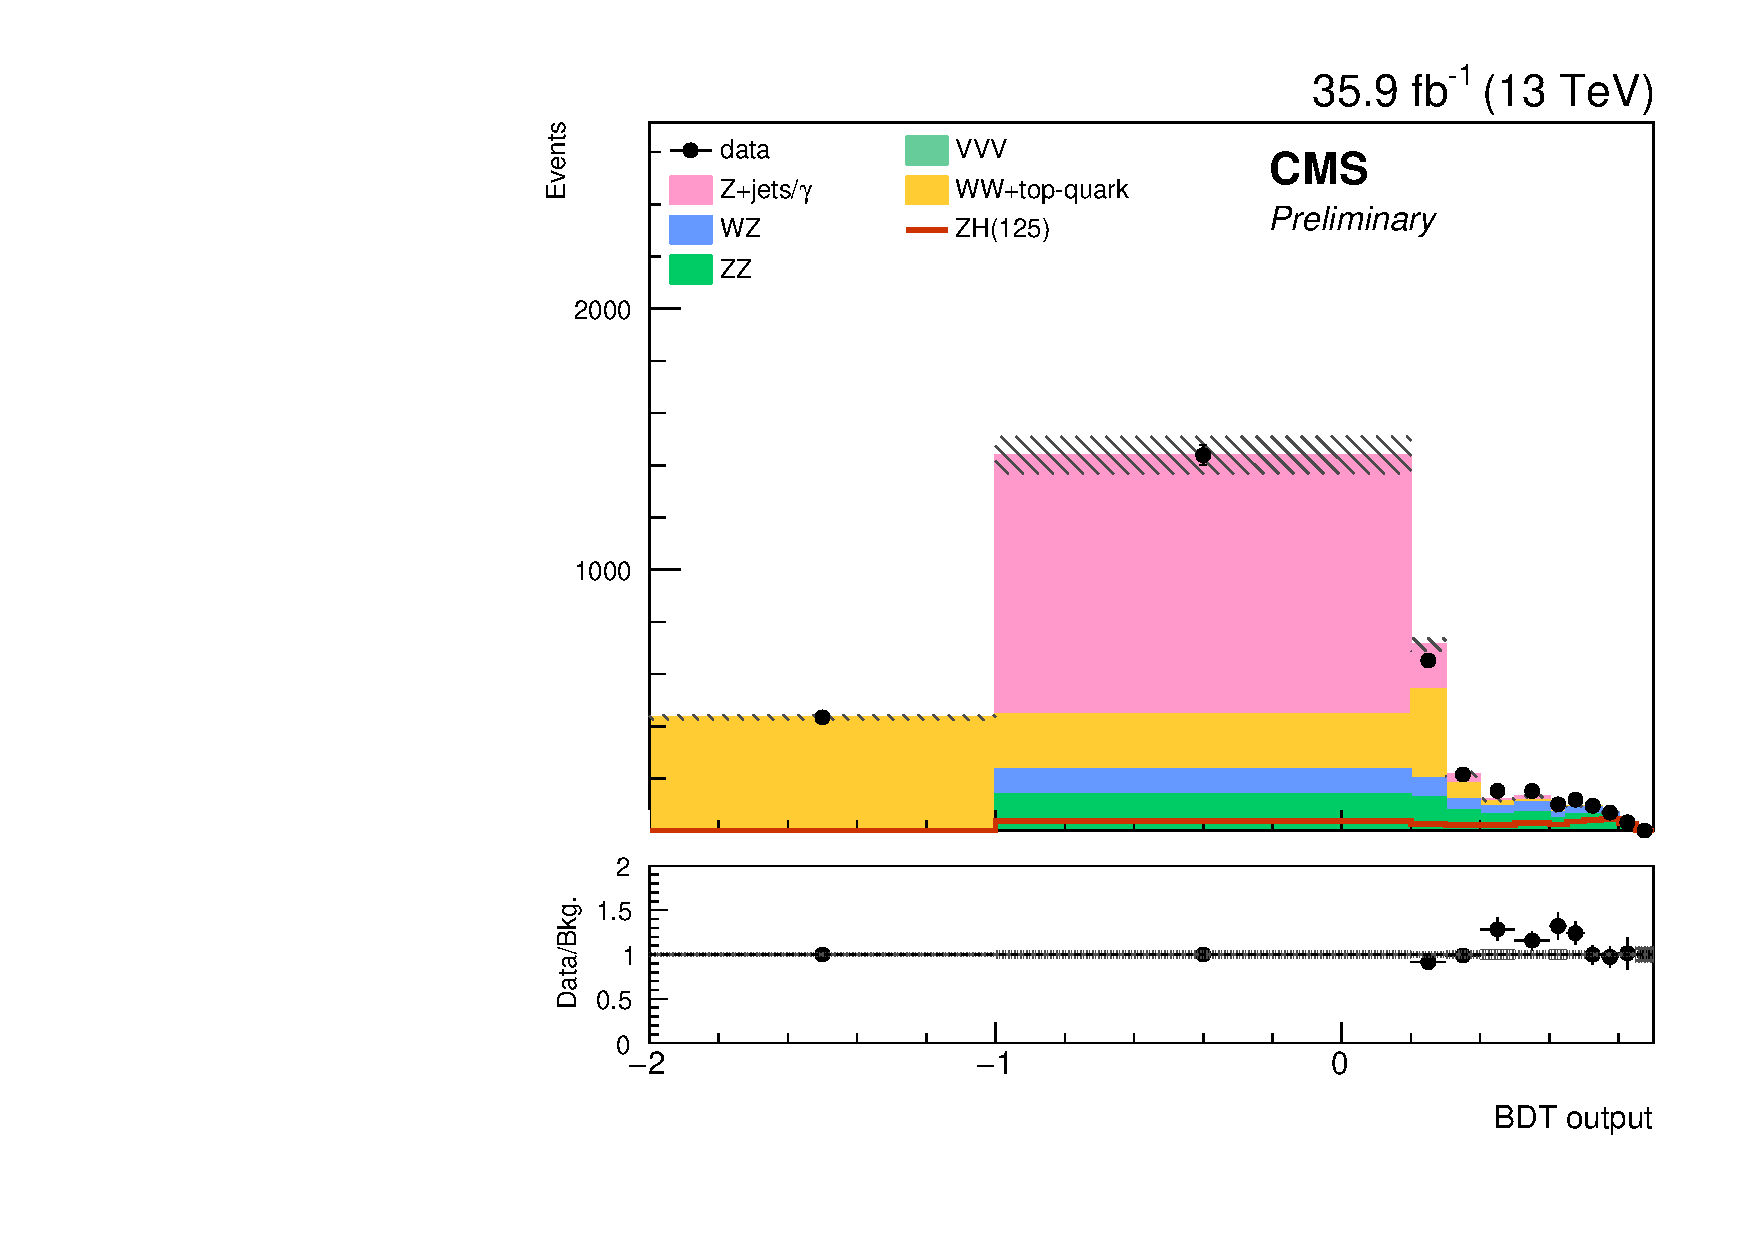
\includegraphics[width=0.48\textwidth]{figures/bdt_zh_prefit.pdf}
\caption{Distribution of the BDT classifier in the multivariate analysis before the likelihood fit.
The first two bins $[-2,\ -1]$ and $[-1,\ 0]$ are a technical artifact of the control region implementation and do not correspond to a BDT score.
The first bin contains the nonresonant background sideband of opposite-flavor events. The second bin contains the Drell-Yan sideband of events failing the BDT or $\met$ requirement. The rest of the bins are the signal region BDT bins. Uncertainty bands represent only the statistical uncertainty.}
\label{fig:bdt_zh_prefit}
\end{center}
\end{figure}

\begin{figure}[htbp]
\begin{center}
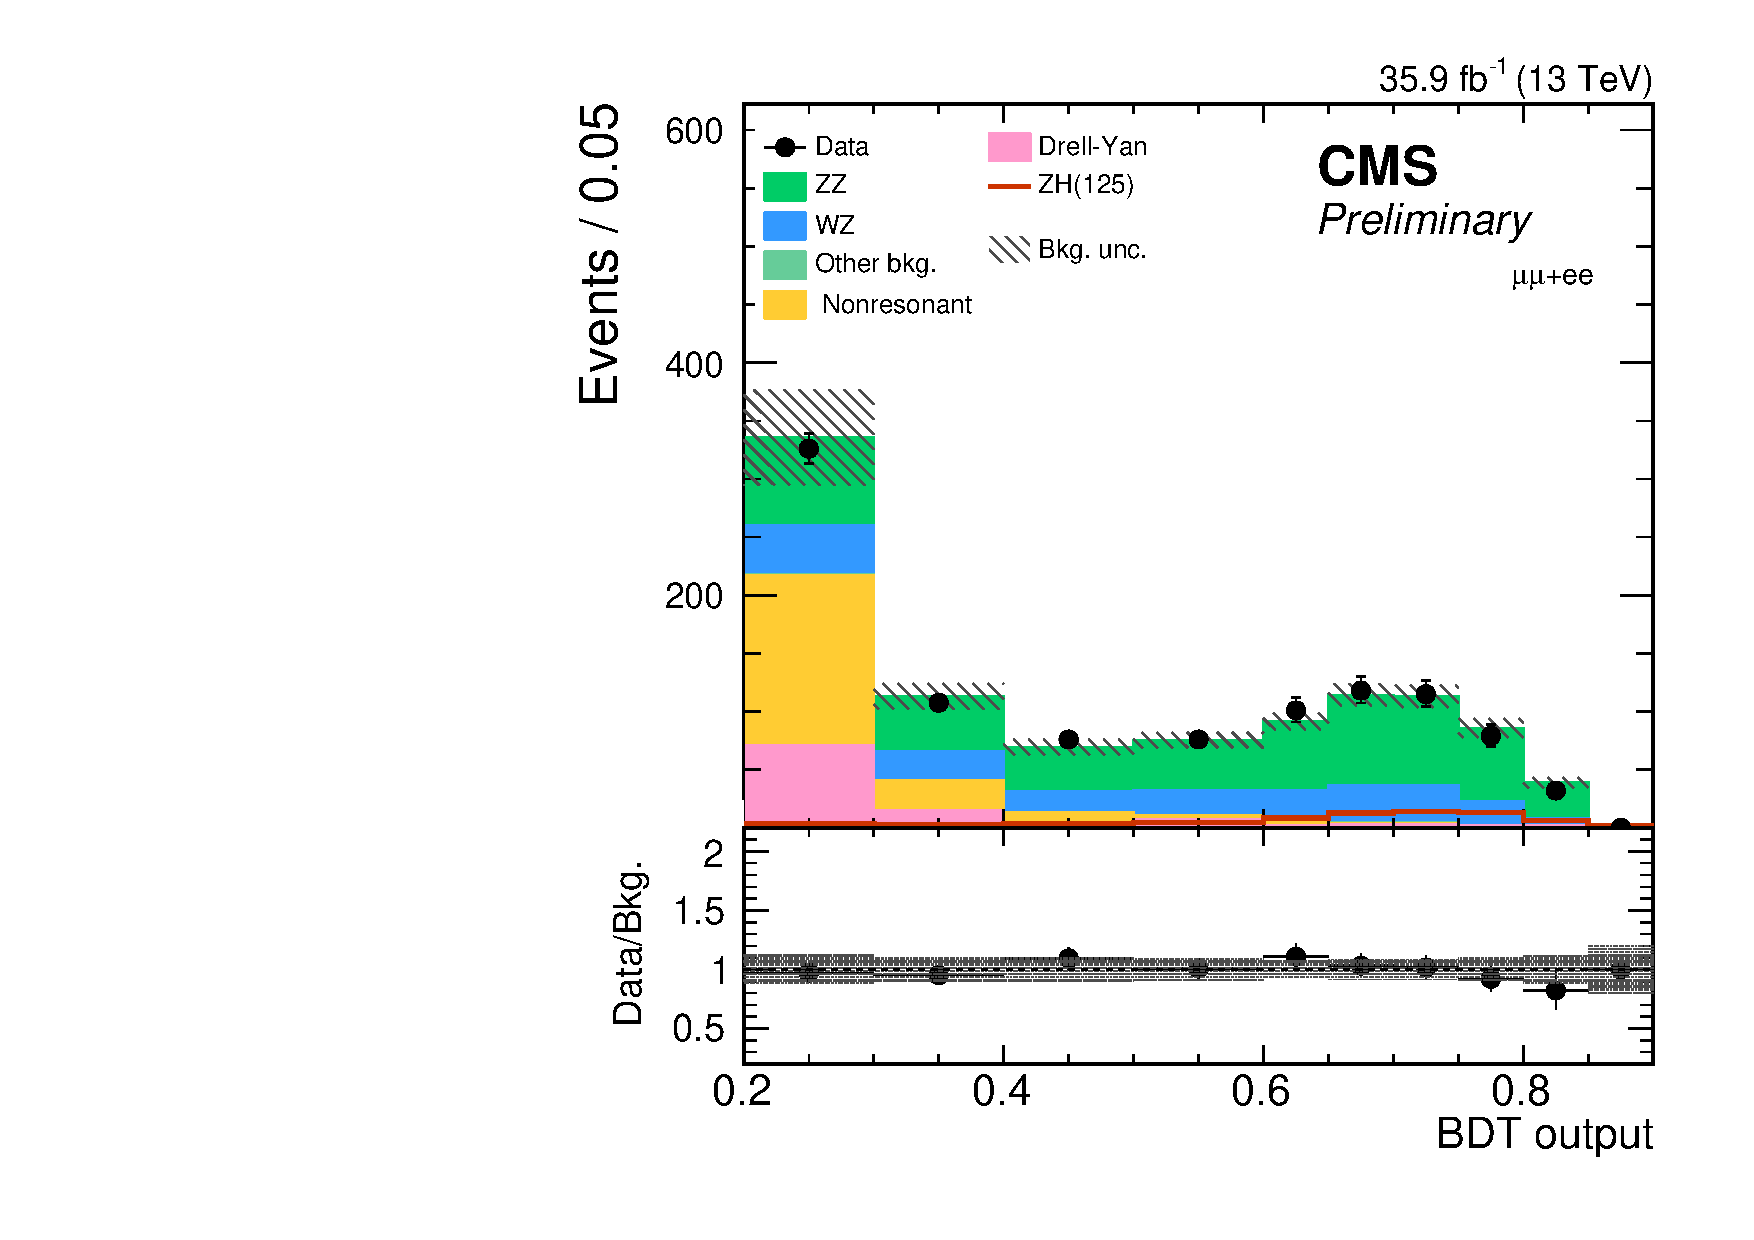
\includegraphics[width=0.48\textwidth]{figures/fullsel_bdt_ll_postfit.pdf}
\caption{Distribution of the BDT classifier in the multivariate analysis signal region after the likelihood fit. Uncertainty bands correspond to both statistical and systematic uncertainty.}
\label{fig:bdt_zh}
\end{center}
\end{figure}

\begin{figure}[htbp]
\begin{center}
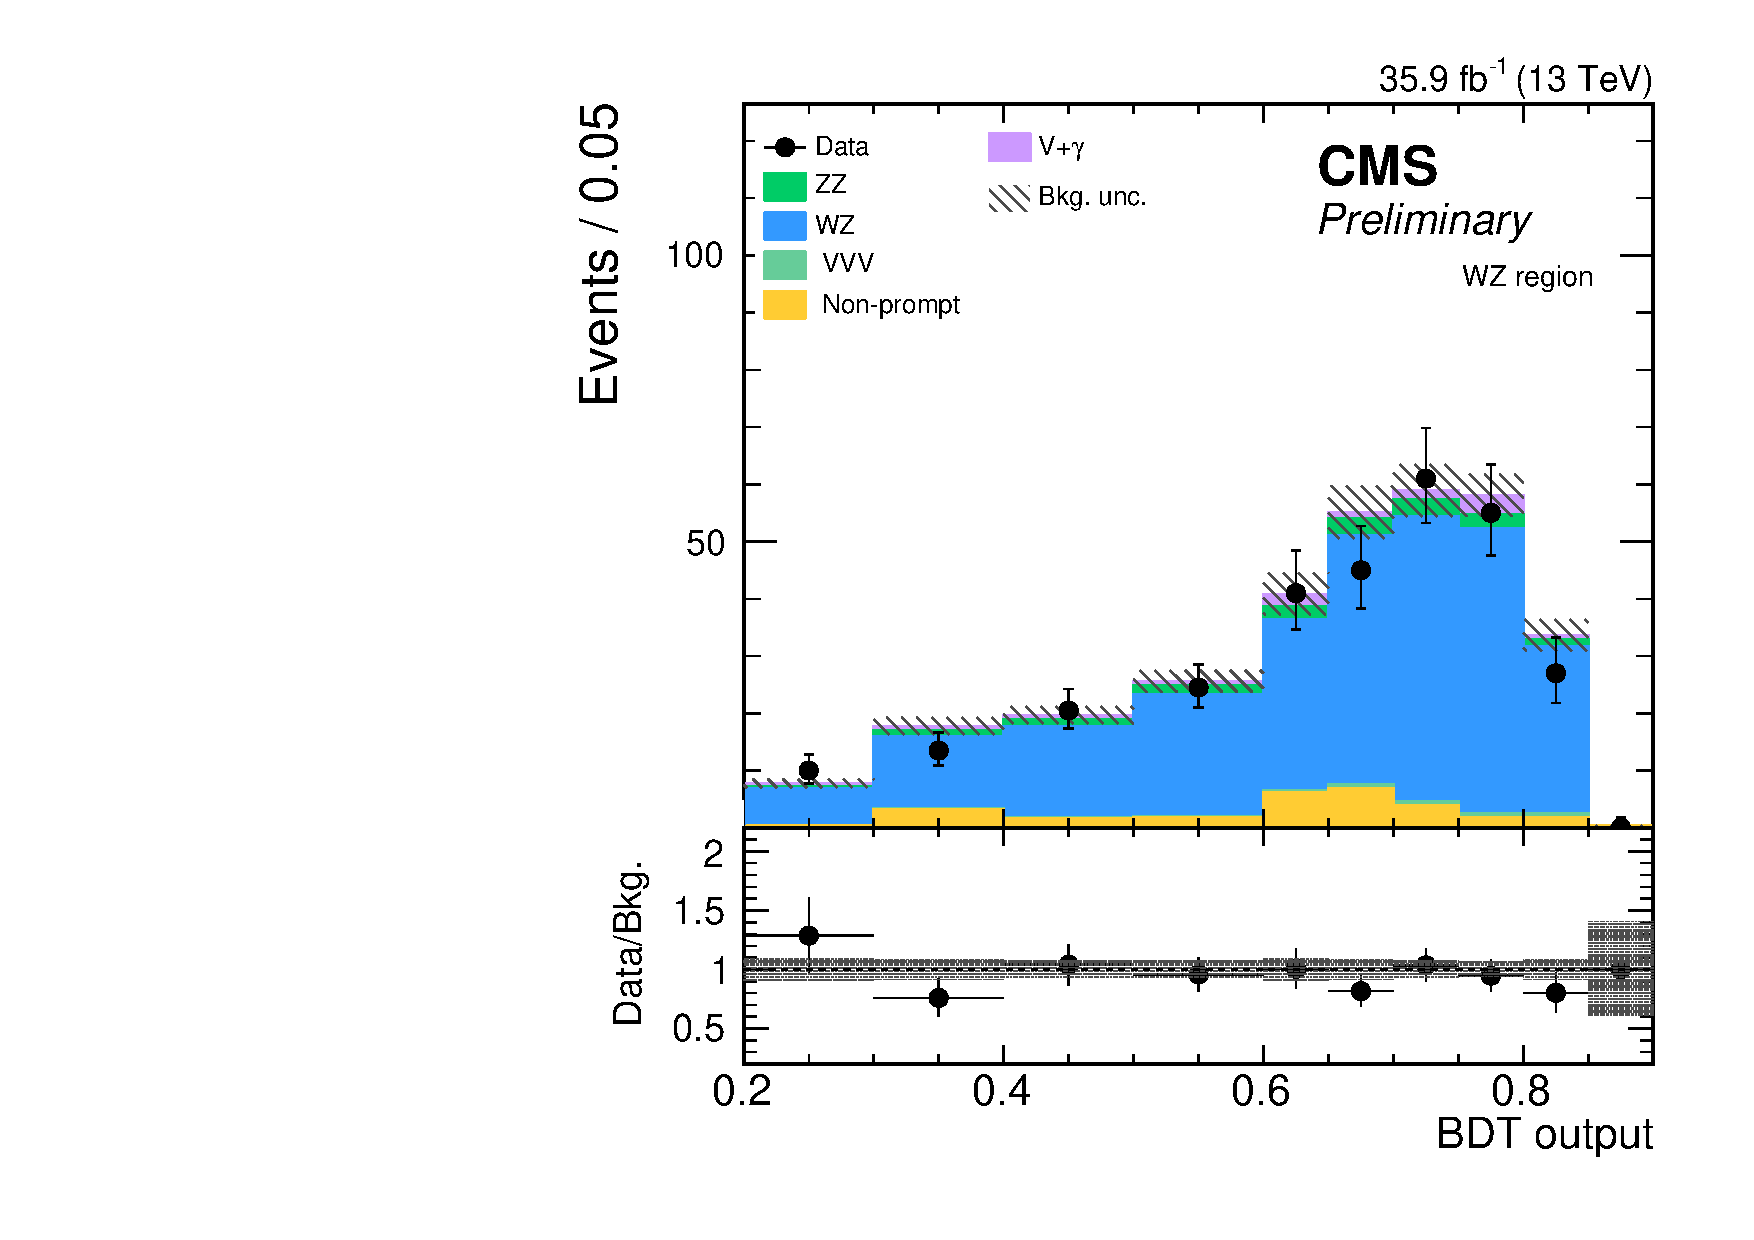
\includegraphics[width=0.48\textwidth]{figures/fullsel_bdt_wz_postfit.pdf}
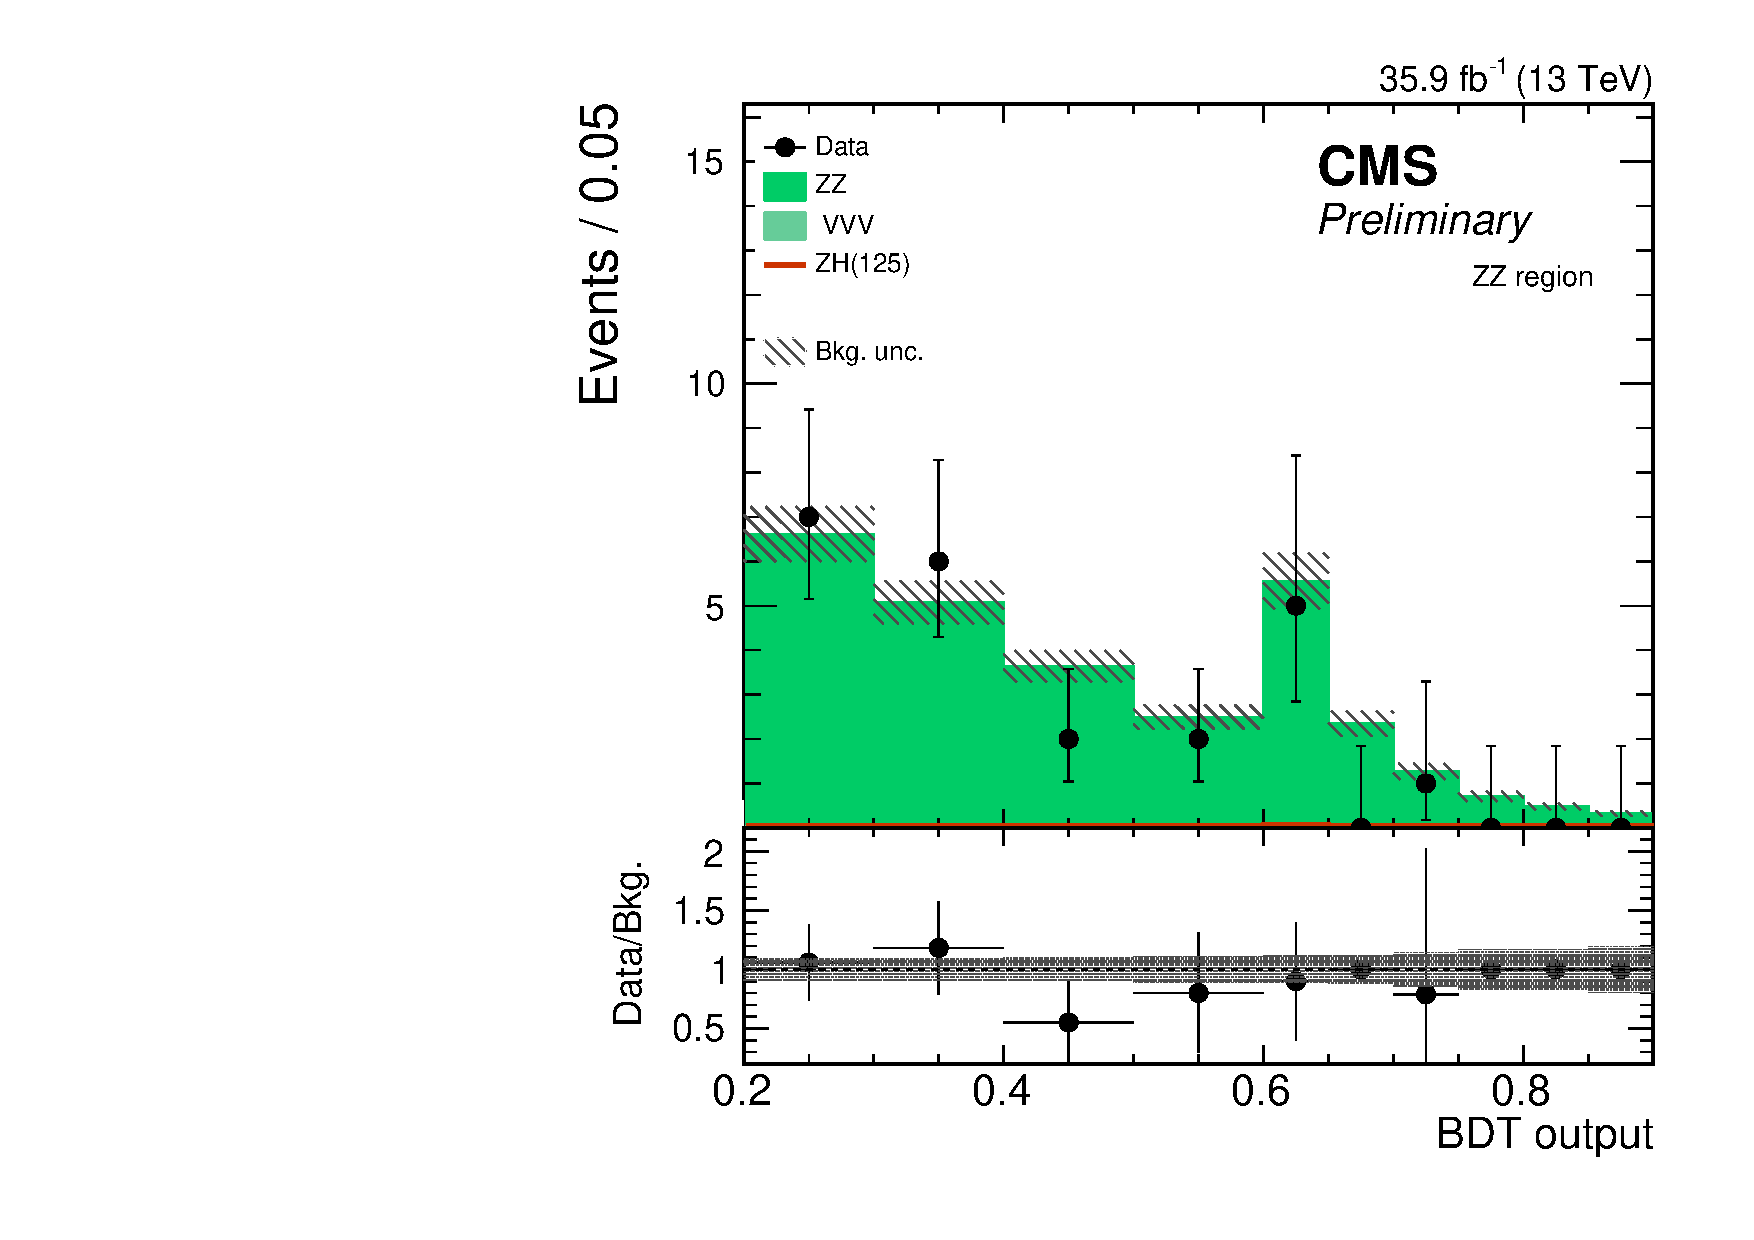
\includegraphics[width=0.48\textwidth]{figures/fullsel_bdt_zz_postfit.pdf}
\caption{Distribution of the BDT classifier in the diboson control regions: WZ three-lepton region at left, ZZ four-lepton region at right. Uncertainty bands correspond to both statistical and systematic uncertainty. 
%These are the same events as shown earlier in Chapter~\ref{chap:dibosons}, Figure \ref{fig:histo_fakemet}.}
These are the same events as in Figure \ref{fig:histo_fakemet}.}
\label{fig:bdt_vv}
\end{center}
\end{figure}
\clearpage

The experimental uncertainties affecting the input values to the BDT are propagated to
the corresponding uncertainties on the output distribution of BDT scores in a robust mapping procedure.
For a discussion of it, see Section \ref{sec:bdt_toys}.

\subsection{Improvement in sensitivity} 
A maximum likelihood fit is performed in the distribution of BDT scores, akin to the $\met$ analysis prescription described in Section~\ref{sec:likelihood}.
The ZZ/WZ ratio is handled in the same way, but the bin-dependent electroweak uncertainty on the ratio of ZZ/WZ
is described in bins of BDT score instead of (emulated) $\met$.
Altogether, the BDT analysis improves the invisible Higgs sensitivity by 10\%,
where the metric is the expected limit on the branching ratio of Higgs boson to invisible particles.

Taking this approach is not nearly as rewarding for the higher mass simplified-model DM signals, where $\met$ is a more powerful discriminant variable.
Furthermore, the multivariate analysis strategy described above is dependent on the mediator mass.
This would necessitate training and evaluating a different classifier for every mass scenario.
These cases require further study before multivariate techniques can be exploited there.

\section{Search results}
\label{sec:dmresults}
The number of observed and expected events after final selection for the $\met$ and BDT analyses are shown in Tables~\ref{tab:zhinvsel} and~\ref{tab:BDTsel}, respectively. 
There is no significant difference between the dimuon and dielectron channels 
in terms of signal-to-background ratio, and hence the two of them 
are treated together when computing the final results. 
Figure~\ref{fig:distributions1} shows the $\met$
distributions after the final selection.

No deviation from the SM background expectations is found.
Upper limits on the contribution of events from new physics are
computed by using the modified frequentist approach
$\CLs$~\cite{Read1,junkcls} based on asymptotic
formulas~\cite{Cowan:2010js}. 
The expected numbers of background events and signal events, scaled by
a signal strength modifier, are combined in a profile-likelihood test 
statistic, in which the systematic uncertainties are incorporated as
nuisance parameters. 
%binned likelihood for each bin of the $\met$ distribution. 
The systematic uncertainties include normalization uncertainties that
affect the overall size of contributions and, when a shape analysis is
performed, shape uncertainties that alter the shapes of the
distributions used in extracting the signal limits. 


\setlength{\tabcolsep}{12pt}
\begin{table}[hbtp]
  \caption{Observed number of events, post-fit background estimates, and signal 
  predictions for the $\met$ analysis using $\usedLumi$. Both statistical and systematic uncertainties are reported.
  High-mass Higgs model is scaled to 1 pb
  (all masses in \GeV).
  \label{tab:zhinvsel}}
  \begin{center}
{\footnotesize
  \begin{tabular}{rlll}
\hline 
Process & ee & $\mu\mu$ & $\mu\mu$+ee \\
\hline
qqZH(125)             &   69.3 $\pm$  2.3 &   89.3 $\pm$  3.1 &  158.6 $\pm$    5.4 \\
ggZH(125)             &   18.4 $\pm$  2.0 &   24.3 $\pm$  2.9 &   42.7 $\pm$    4.9 \\
ZH(800)               &  113.1 $\pm$  4.5 &  152.1 $\pm$  6.1 &  265.1 $\pm$   10.6 \\
DM(150)MV(500)        &   40.9 $\pm$  1.6 &   57.9 $\pm$  2.3 &   98.8 $\pm$    3.9 \\
DM(150)MA(500)        &   27.5 $\pm$  1.1 &   38.0 $\pm$  1.5 &   65.5 $\pm$    2.6 \\
\hline
Nonresonant bkg.      &   32.1 $\pm$  6.4 &   41.0 $\pm$  8.2 &   74.8 $\pm$	15.0 \\ 
$ZZ$                  &  162.3 $\pm$  4.0 &  217.5 $\pm$  5.4 &  379.8 $\pm$	 9.4 \\ 
$WZ\rightarrow3l\nu$  &   70.4 $\pm$  2.9 &   92.1 $\pm$  3.9 &  162.5 $\pm$	 6.8 \\ 
Other bkg.            &    1.1 $\pm$  0.1 &    1.4 $\pm$  0.1 &    2.6 $\pm$	 0.2 \\ 
Z+Jets                &   35.6 $\pm$ 14.4 &   22.9 $\pm$  9.3 &   72.0 $\pm$	29.2 \\ 
\hline 
Total bkg.            &  310.4 $\pm$ 19.5 &  381.3 $\pm$ 15.7 &  691.7 $\pm$   34.8 \\
\hline 
Data                  &  292              &  396              &  688                 \\
\hline
  \end{tabular}
}
  \end{center}
\end{table}
\begin{table}[hbtp]
  \caption{Observed number of events, post-fit background estimates, and signal 
  predictions for the BDT analysis using $\usedLumi$. Both statistical and systematic uncertainties are reported.
  (all masses in \GeV).
  \label{tab:BDTsel}}
  \begin{center}
{\footnotesize
  \begin{tabular}{rlll}
\hline 
Process & ee & $\mu\mu$ & $\mu\mu$+ee \\
\hline
qqZH(125)             &   89.6 $\pm$  2.5 &  117.3 $\pm$  3.3 &  207.0 $\pm$    5.8 \\
ggZH(125)             &   26.8 $\pm$  2.8 &   35.9 $\pm$  3.7 &   62.7 $\pm$    6.5 \\
\hline
Nonresonant bkg.      &    165 $\pm$   20 &    211 $\pm$   26 &    375 $\pm$	 46 \\ 
$ZZ$                  &    309 $\pm$   12 &    421 $\pm$   17 &    730 $\pm$	 29 \\ 
$WZ\rightarrow3l\nu$  &  142.9 $\pm$  5.2 &  192.5 $\pm$  7.0 &    335 $\pm$	 12 \\ 
Other bkg.            &   2.31 $\pm$ 0.15 &   3.23 $\pm$ 0.21 &   5.54 $\pm$   0.36 \\ 
Z+Jets                &     84 $\pm$   25 &    110 $\pm$   33 &    194 $\pm$	 58 \\ 
\hline 
Total bkg.            &    704 $\pm$   35 &    936 $\pm$   46 &   1640 $\pm$     81 \\
\hline 
Data                  &    682 $\pm$   26 &    904 $\pm$   30 &   1586 $\pm$     40 \\
\hline
  \end{tabular}
}
  \end{center}
\end{table}
\setlength{\tabcolsep}{6pt}

\begin{figure}[hbtp]
\begin{center}
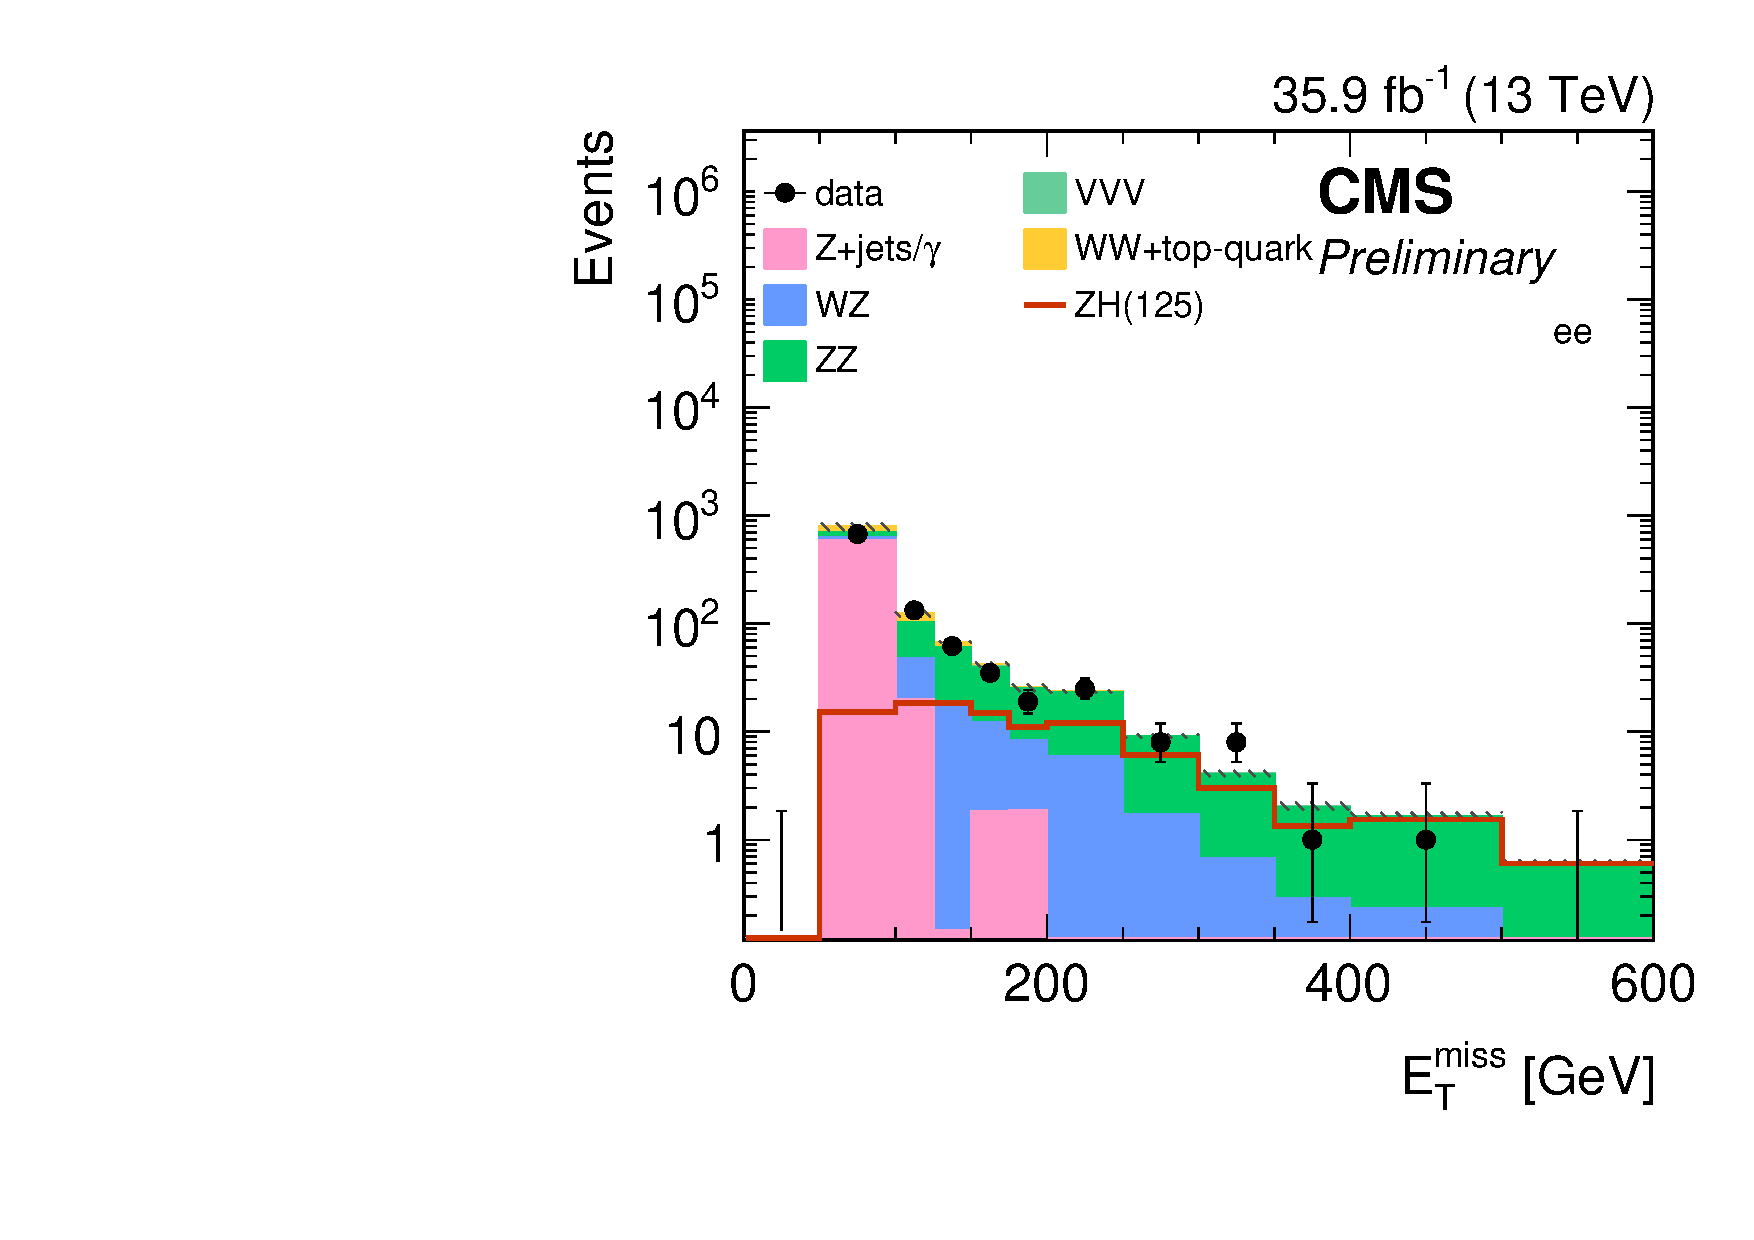
\includegraphics[height=0.3\textheight,width=\cmsFigWidth]{figures/fullsel_met_ee.pdf}
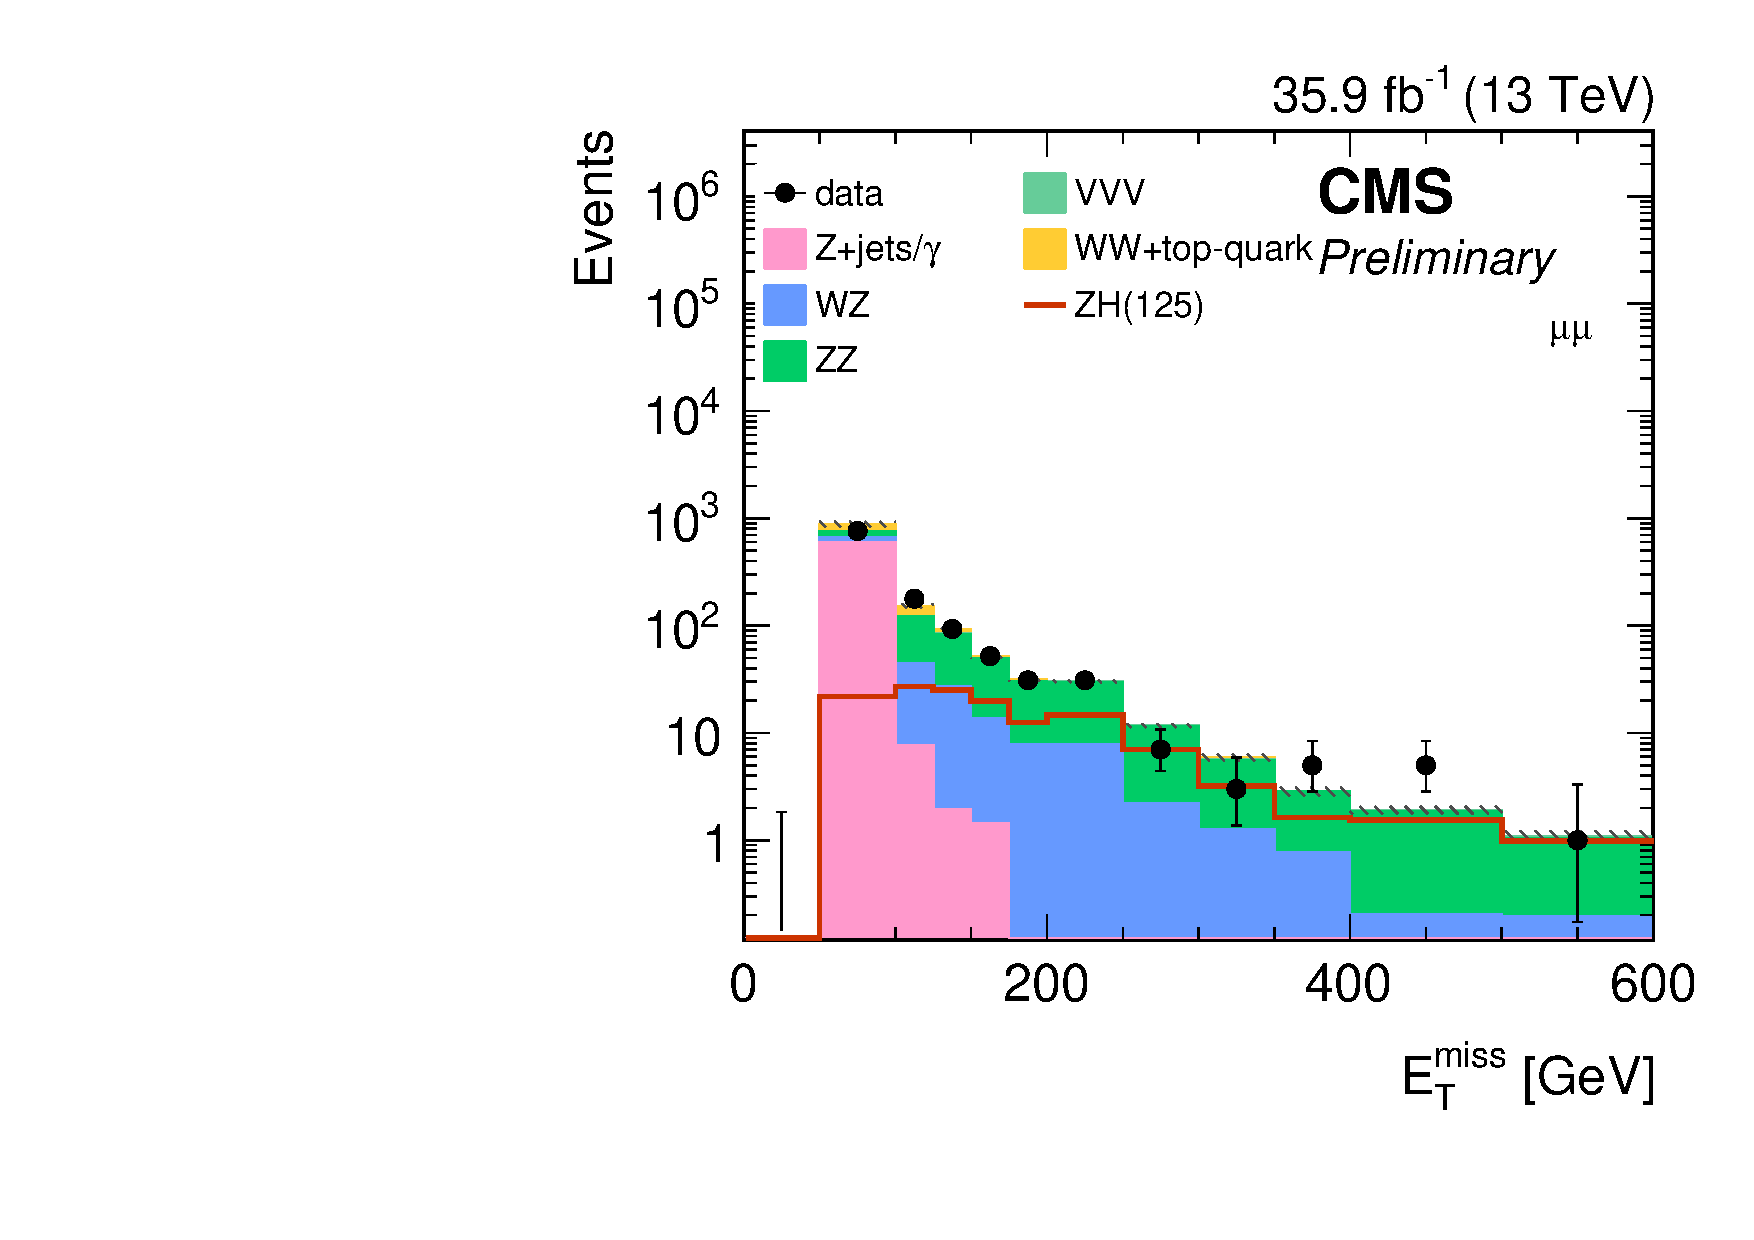
\includegraphics[height=0.3\textheight,width=\cmsFigWidth]{figures/fullsel_met_mm.pdf} \\
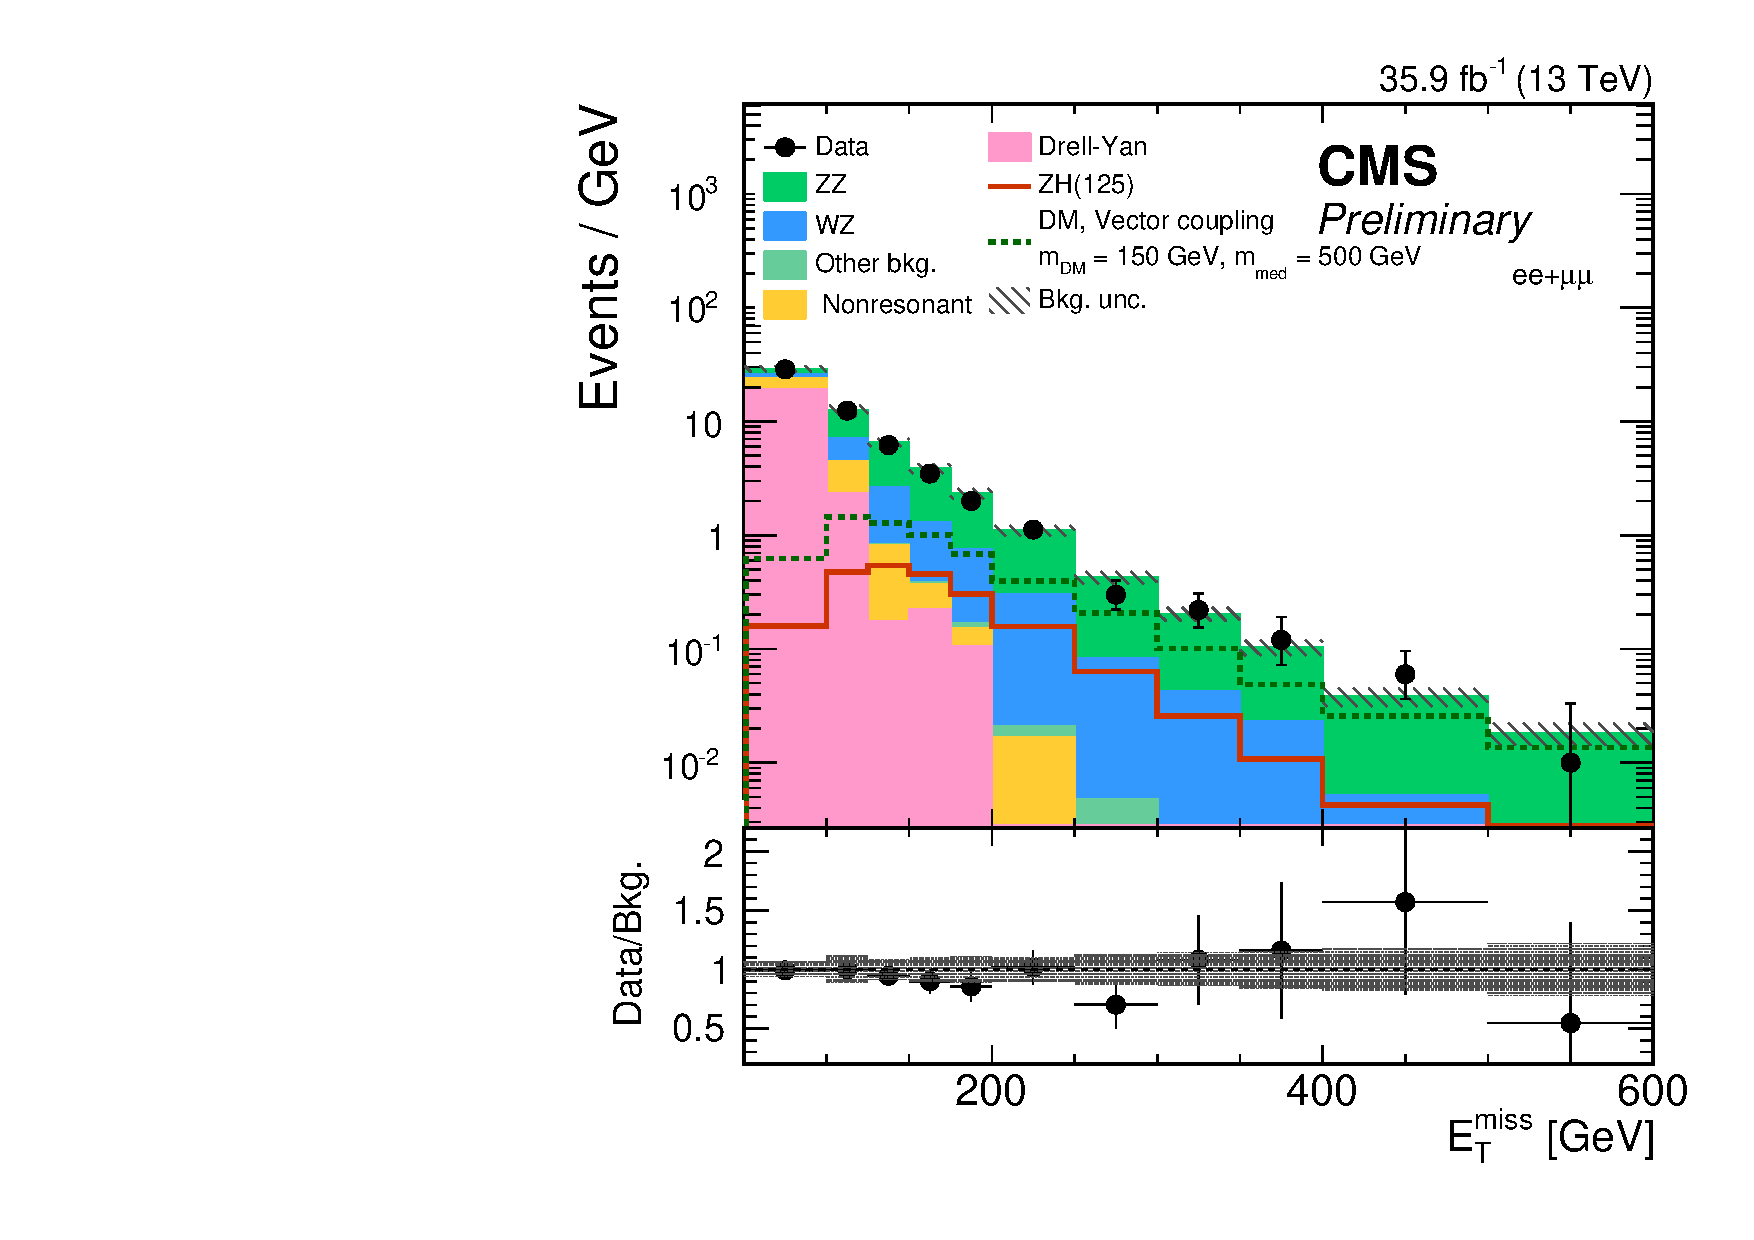
\includegraphics[height=0.3\textheight,width=\cmsFigWidth]{figures/fullsel_met_ll_postfit.pdf}
\caption{Distribution of the $\met$ after the full selection including the region between 50 and 100 $\GeV$.
  For the ee channel (top left) and $\mu\mu$ channel (top right), the uncertainty band corresponds to the statistical uncertainty only.
  For the $\ell\ell$ channel (bottom), the plot includes both statistical and systematic uncertainty.
  The signal normalization is arbitrary.}
\label{fig:distributions1}
\end{center}
\end{figure}

\begin{figure}[hbtp]
\begin{center}
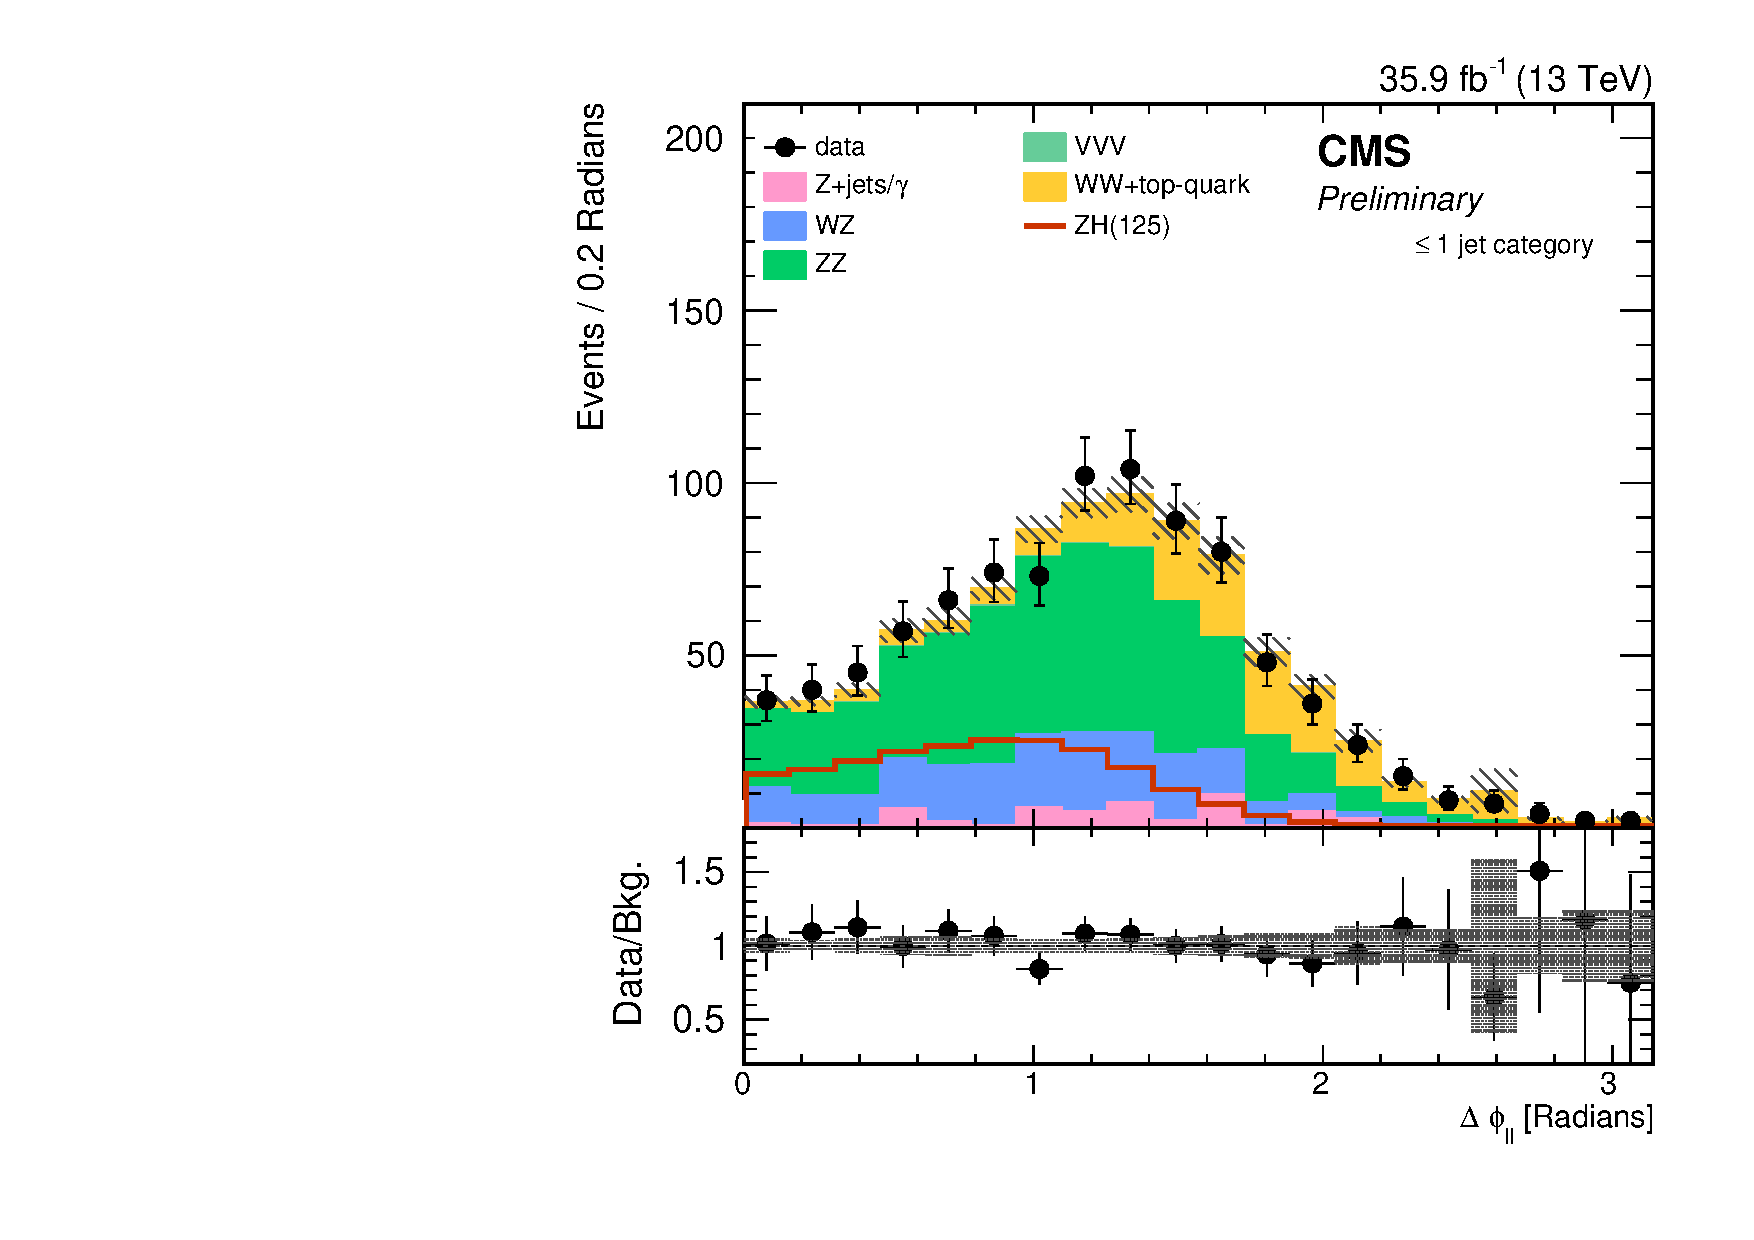
\includegraphics[width=\cmsFigWidth]{figures/zh_1j_deltaphill_allcutsbutone.pdf}
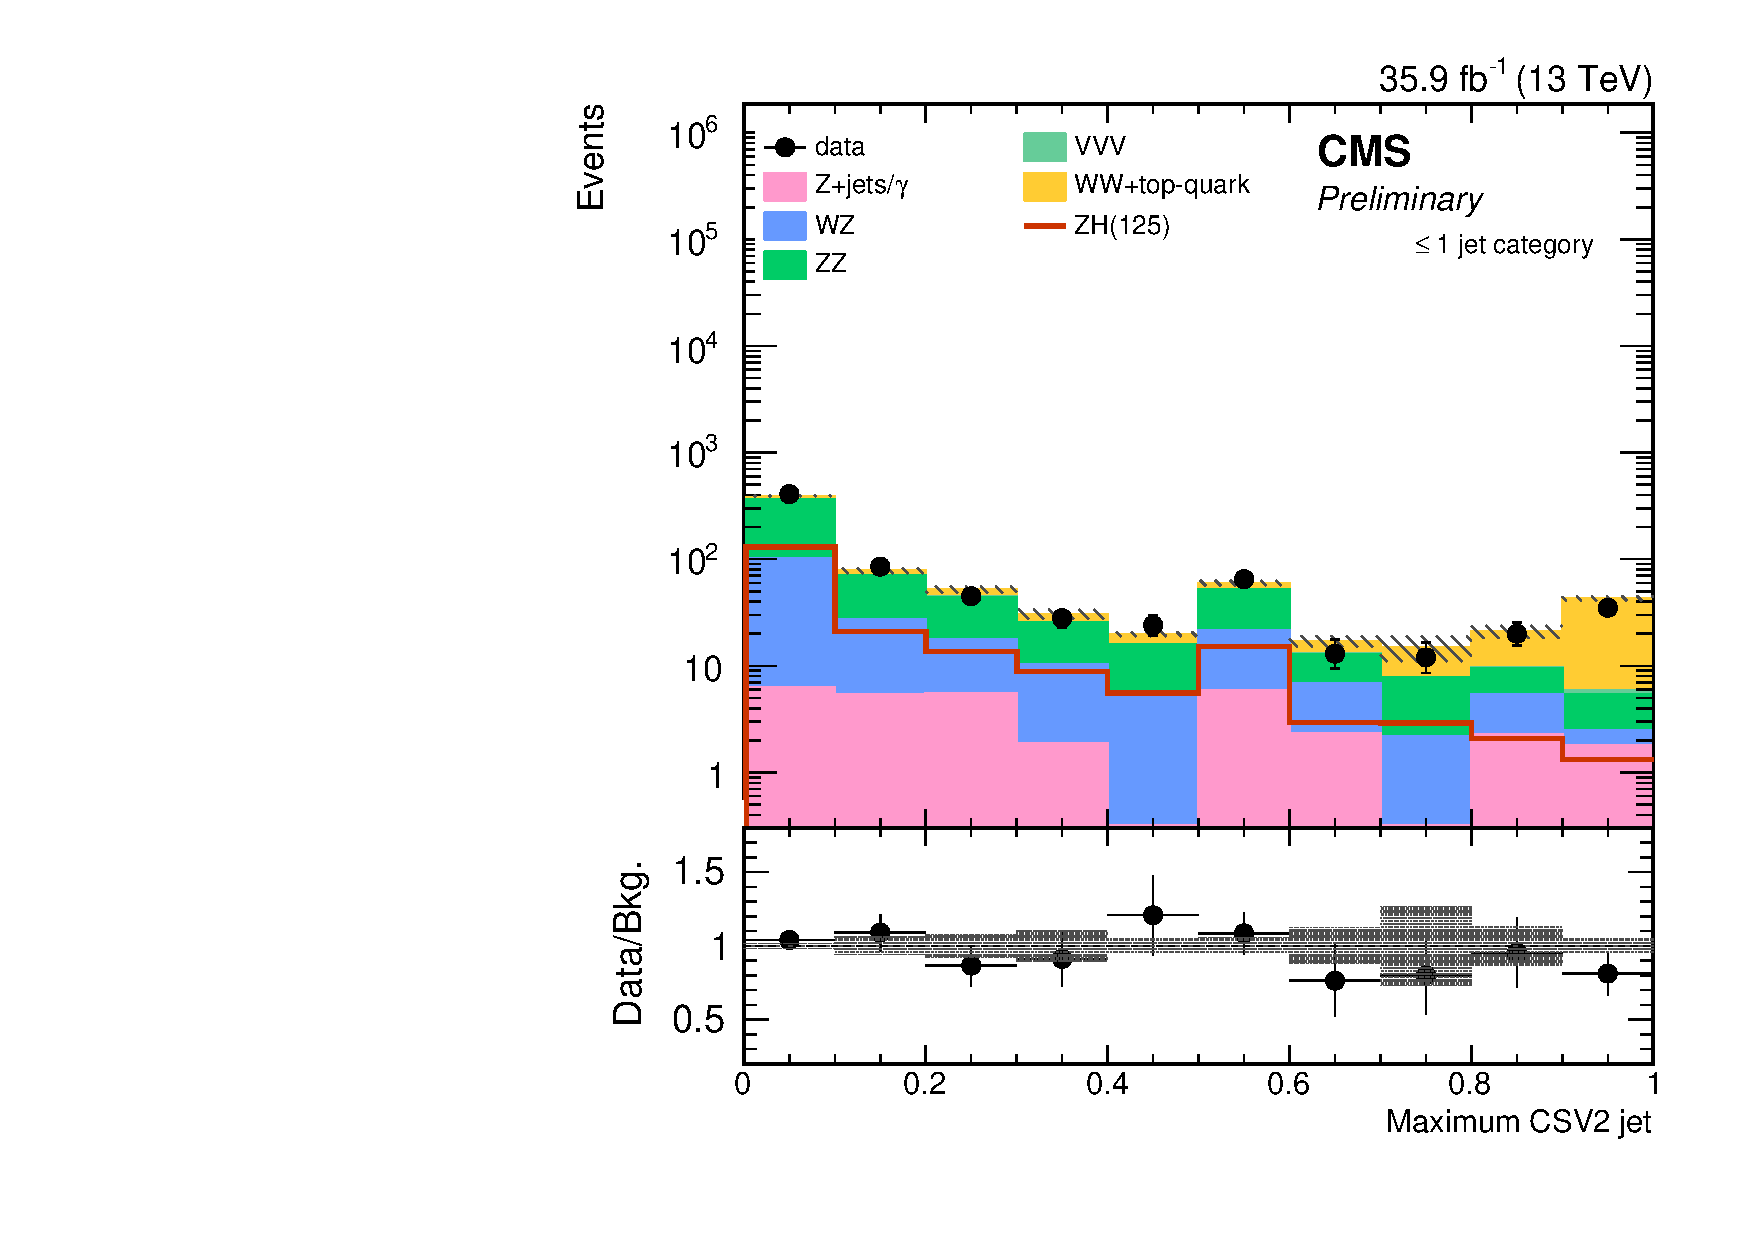
\includegraphics[width=\cmsFigWidth]{figures/zh_1j_btagmax_allcutsbutone.pdf}
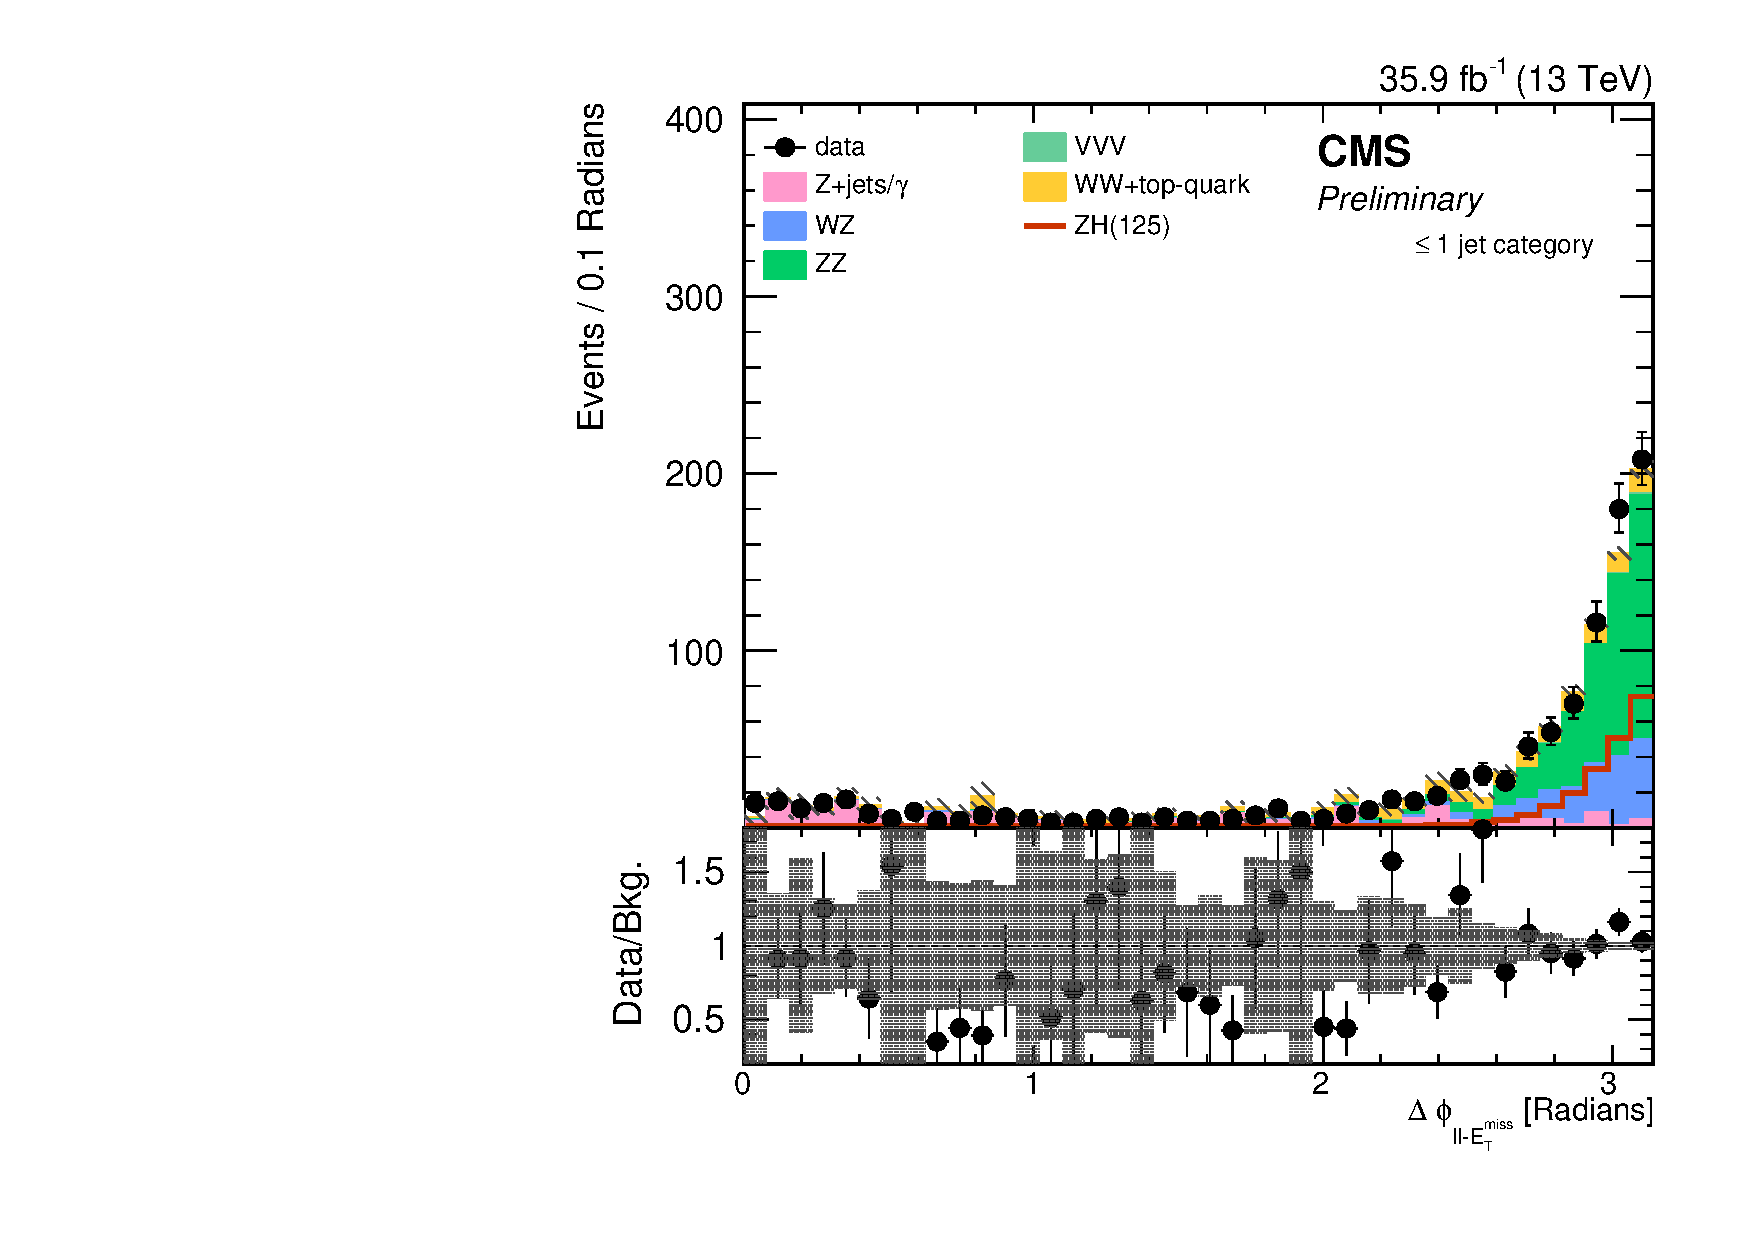
\includegraphics[width=\cmsFigWidth]{figures/zh_1j_dphillmet_allcutsbutone.pdf}
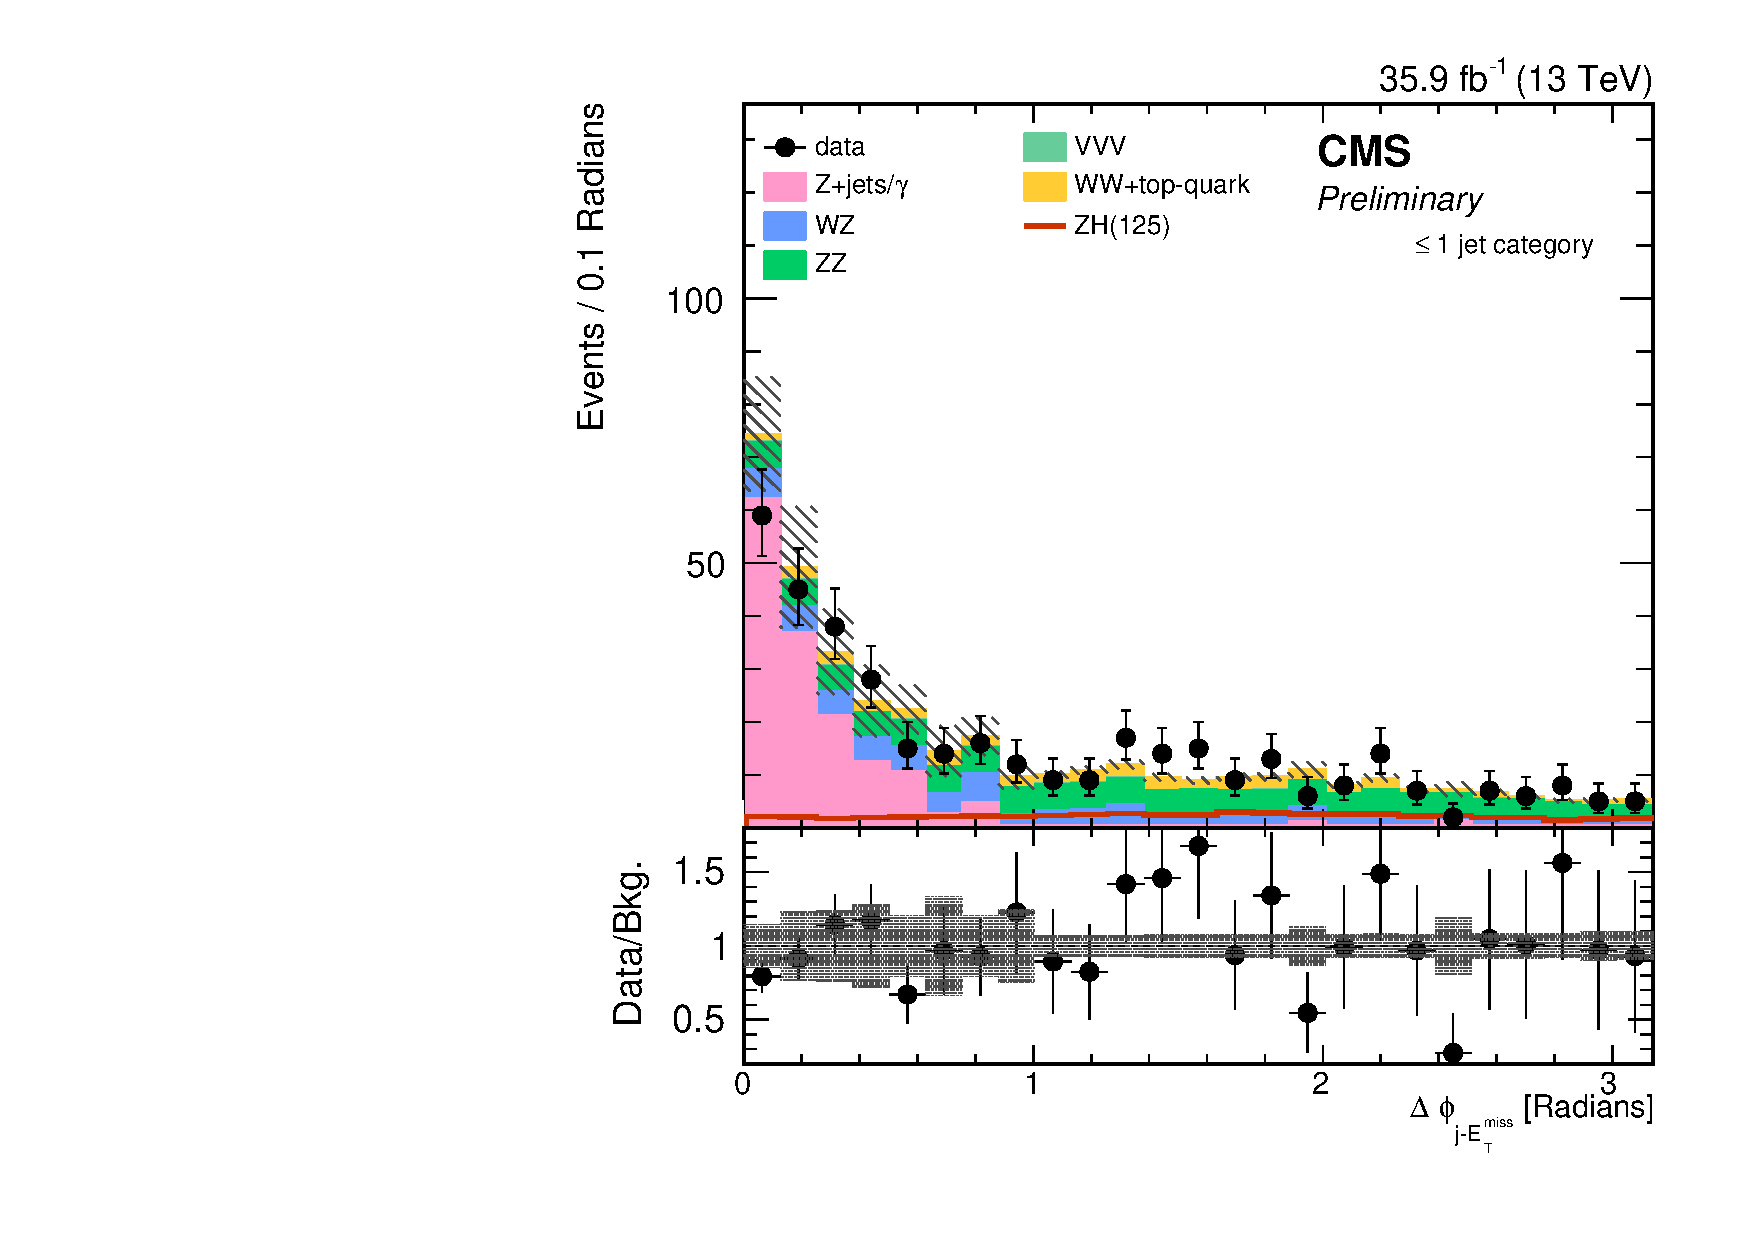
\includegraphics[width=\cmsFigWidth]{figures/zh_1j_dphijmet_allcutsbutone.pdf}
\caption{Distributions after the full selection except the variable itself.
Upper left: $\delphill$. 
Upper right: maximum CSV2 b-tagging score among the jets.
Bottom left: $\Delta \phi_{\ell,\met}$.
Bottom right: $\Delta \phi_{{\rm jet},\met}$.
The uncertainty band corresponds to the statistical uncertainty only.}
\label{fig:distributions2}
\end{center}
\end{figure}


%%%%%%%%%%%%%%%%%%%%%%%%%%%%%%%%%%%%%%%%%%%%%%%%%%%%%%%% 
%%%%%%%%%%%%%%%%%%%%%%%%%%%%%%%%%%%%%%%%%%%%%%%%%%%%%%%%
\clearpage
\subsection{Invisible Higgs interpretation} 

No significant excess of events is observed over the SM expectation.
Upper limits are derived for the Higgs boson production cross section.
For  $\mHi = 125~\GeV$, this is interpreted as the upper limit on the
branching ratio of the Higgs boson to invisible particles,
assuming the SM production rate. 
To compute the upper limits, the modified frequentist construction 
$\CLs$ is used (see ~\cite{Read1,junkcls,ATLAS:2011tau}).
The number of events are modeled as a Poisson random variable, 
where the mean value is the sum of the contributions from signal and background processes. 
The 95\% observed and median expected CL upper limits on the production cross section times branching ratio, 
$\sigma_{qq \to \Z \Hi} \times \mathrm{B}(\Hi \to {\rm invisible})$, computed with the asymptotic $\CLs$
method are shown in Figure~\ref{fig:xsLim} for the rectangular analysis in $\met$.
Assuming the SM production rate, the 95\% observed (expected) CL upper limit on $\mathrm{B}(\Hi \to {\rm invisible})$ is
0.45 (0.44) using the rectangular analysis in \met, and 0.40 (0.42) using the multivariate analysis. 
The $gg \to \Z(\ell\ell)\Hi$ process has also been considered for the 125 GeV mass point. 

The signal strength limits for quark+gluon initiated $\Z\Hi(\to{\rm invisible})$ processes is shown in Fig.~\ref{fig:xsLim_qqgg}.
The signal strength limits for only quark-initiated processes is shown in Fig.~\ref{fig:xsLim_qq}.


%\begin{figure}[bhp]
%  \floatbox[{\capbeside\thisfloatsetup{capbesideposition={right,bottom},capbesidewidth=4.75cm}}]{figure}[\FBwidth]
%  {\caption{
%   Expected and observed 95\% CL upper 
%   limits on the production cross section times branching ratio, 
%   $\sigma_{\Z\Hi(\to \rm invisible)} \times \mathrm{BR}(\Hi \to {\rm invisible})$
%   as a function of the Higgs boson mass.}
%   \label{fig:xsLim}
%  }
%  {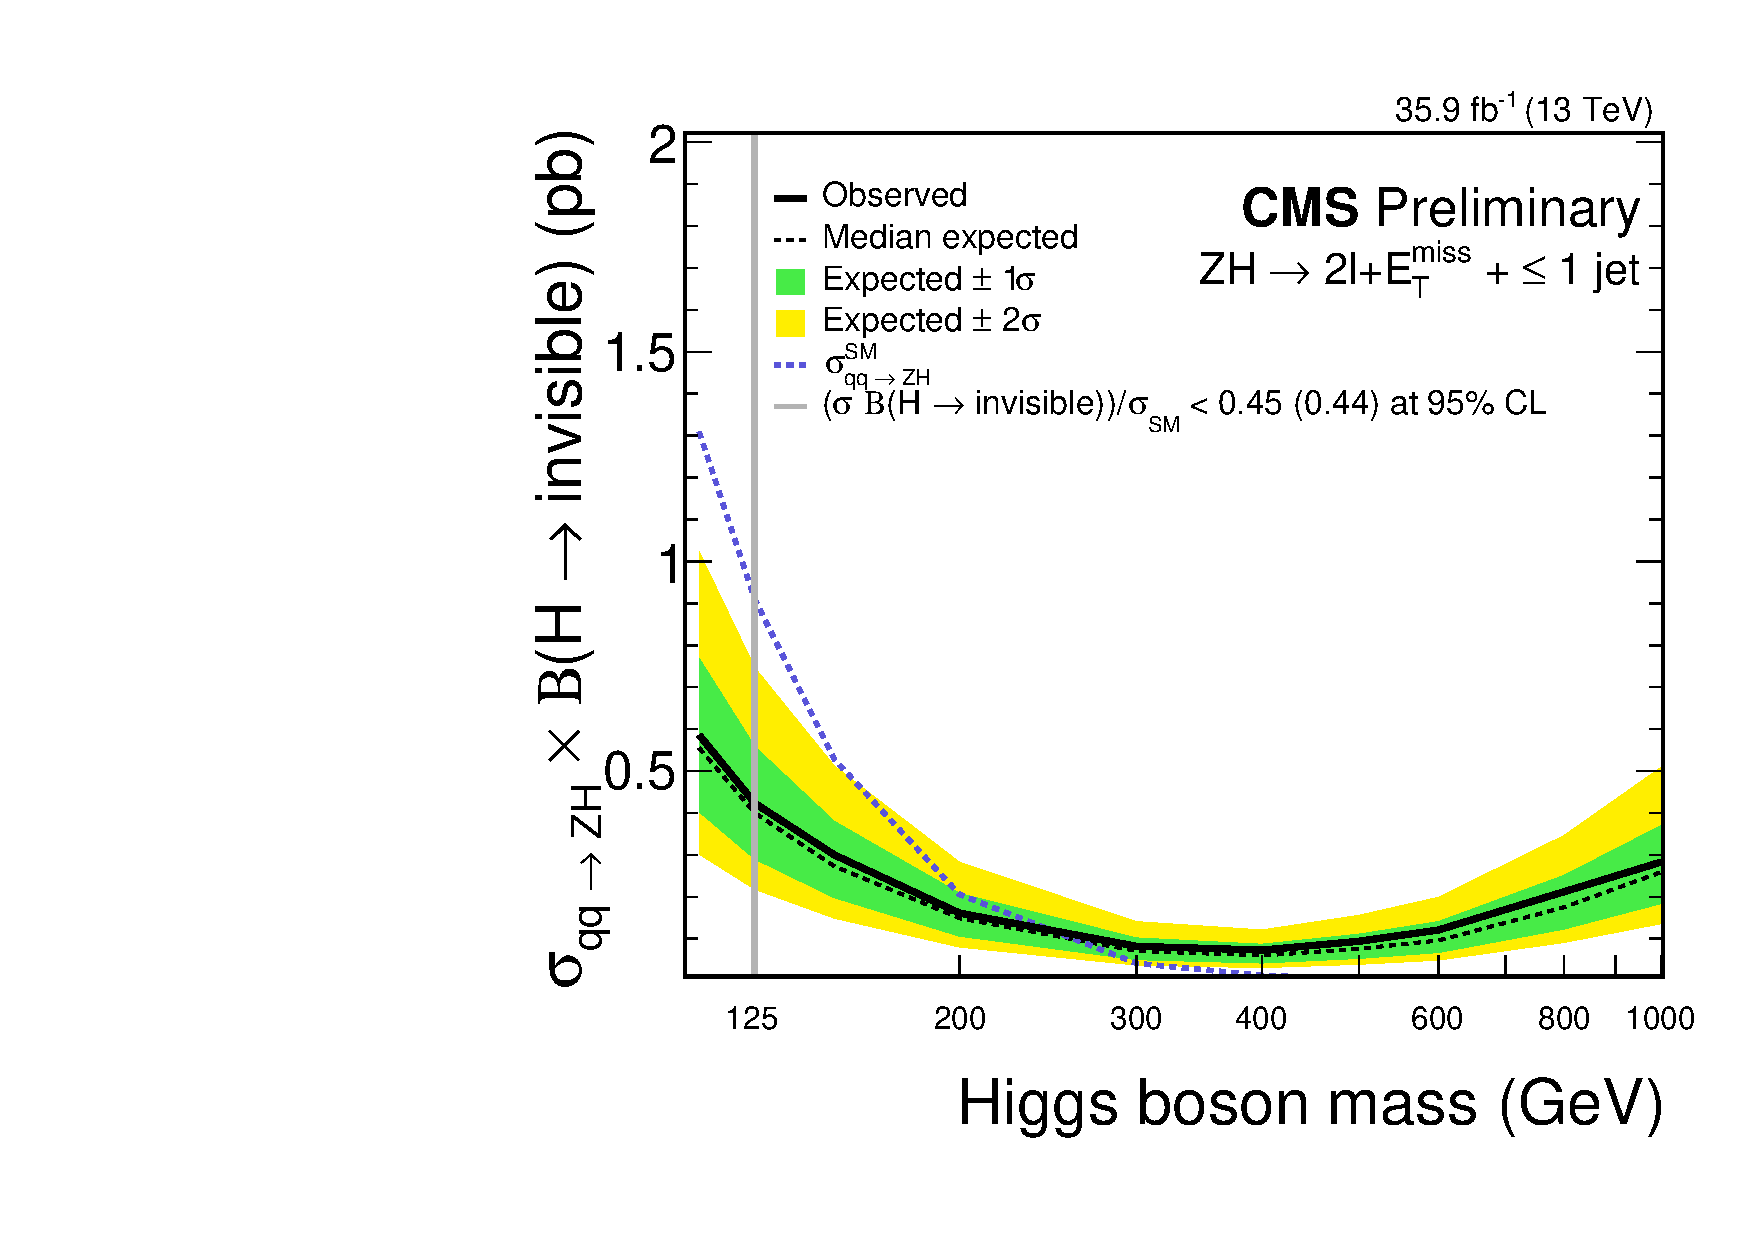
\includegraphics[width=0.55\textwidth]{figures/ana_hzinv_met_nj_from110to1000_logx1_logy0.pdf}}
%\end{figure}

%\begin{figure}[hp]
%  \floatbox[{\capbeside\thisfloatsetup{capbesideposition={right,bottom},capbesidewidth=4.75cm}}]{figure}[\FBwidth]
%  {\caption{
%   Expected and observed 95\% CL upper limits on the signal strength, 
%   $\sigma_{\Z\Hi(\to \rm invisible)} \times \mathrm{BR}(\Hi \to {\rm invisible})/\sigma_{SM}$ as a function of the Higgs boson mass.
%   $\sigma_{SM}$ includes both quark- and gluon-initiated processes.}
%   \label{fig:xsLim_qqgg}
%  }
%  {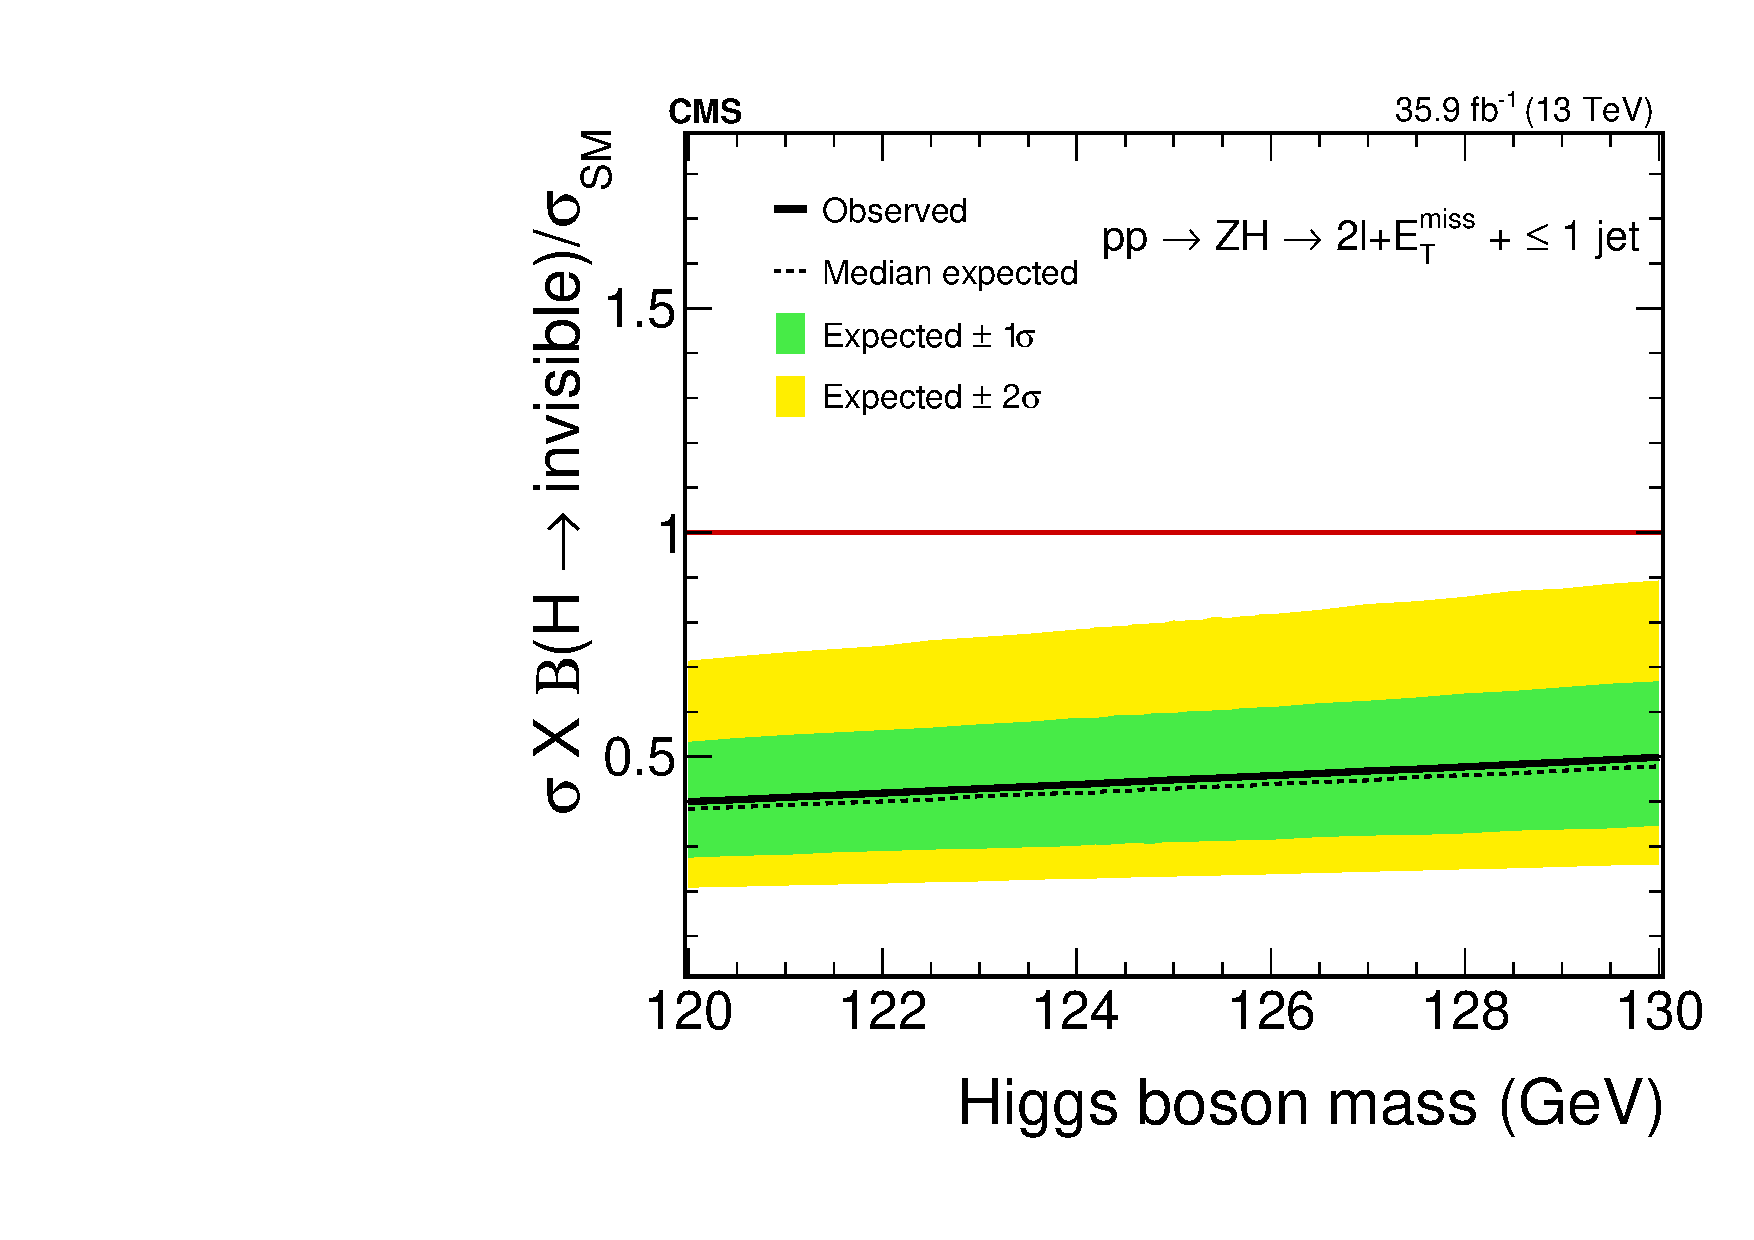
\includegraphics[width=0.55\textwidth]{figures/ana_hzinv_met_nj_massscan_from120to130_logx0_logy0.pdf}}
%\end{figure}
%
%
%\begin{figure}[hp]
%  \floatbox[{\capbeside\thisfloatsetup{capbesideposition={right,bottom},capbesidewidth=4.75cm}}]{figure}[\FBwidth]
%  {\caption{
%   Expected and observed 95\% CL upper limits on the signal strength, 
%   $\sigma_{\Z\Hi(\to \rm invisible)} \times \mathrm{BR}(\Hi \to {\rm invisible})/\sigma_{SM}$ as a function of the Higgs boson mass,
%   including only quark-initiated processes.}
%   \label{fig:xsLim_qq}
%  }
%  {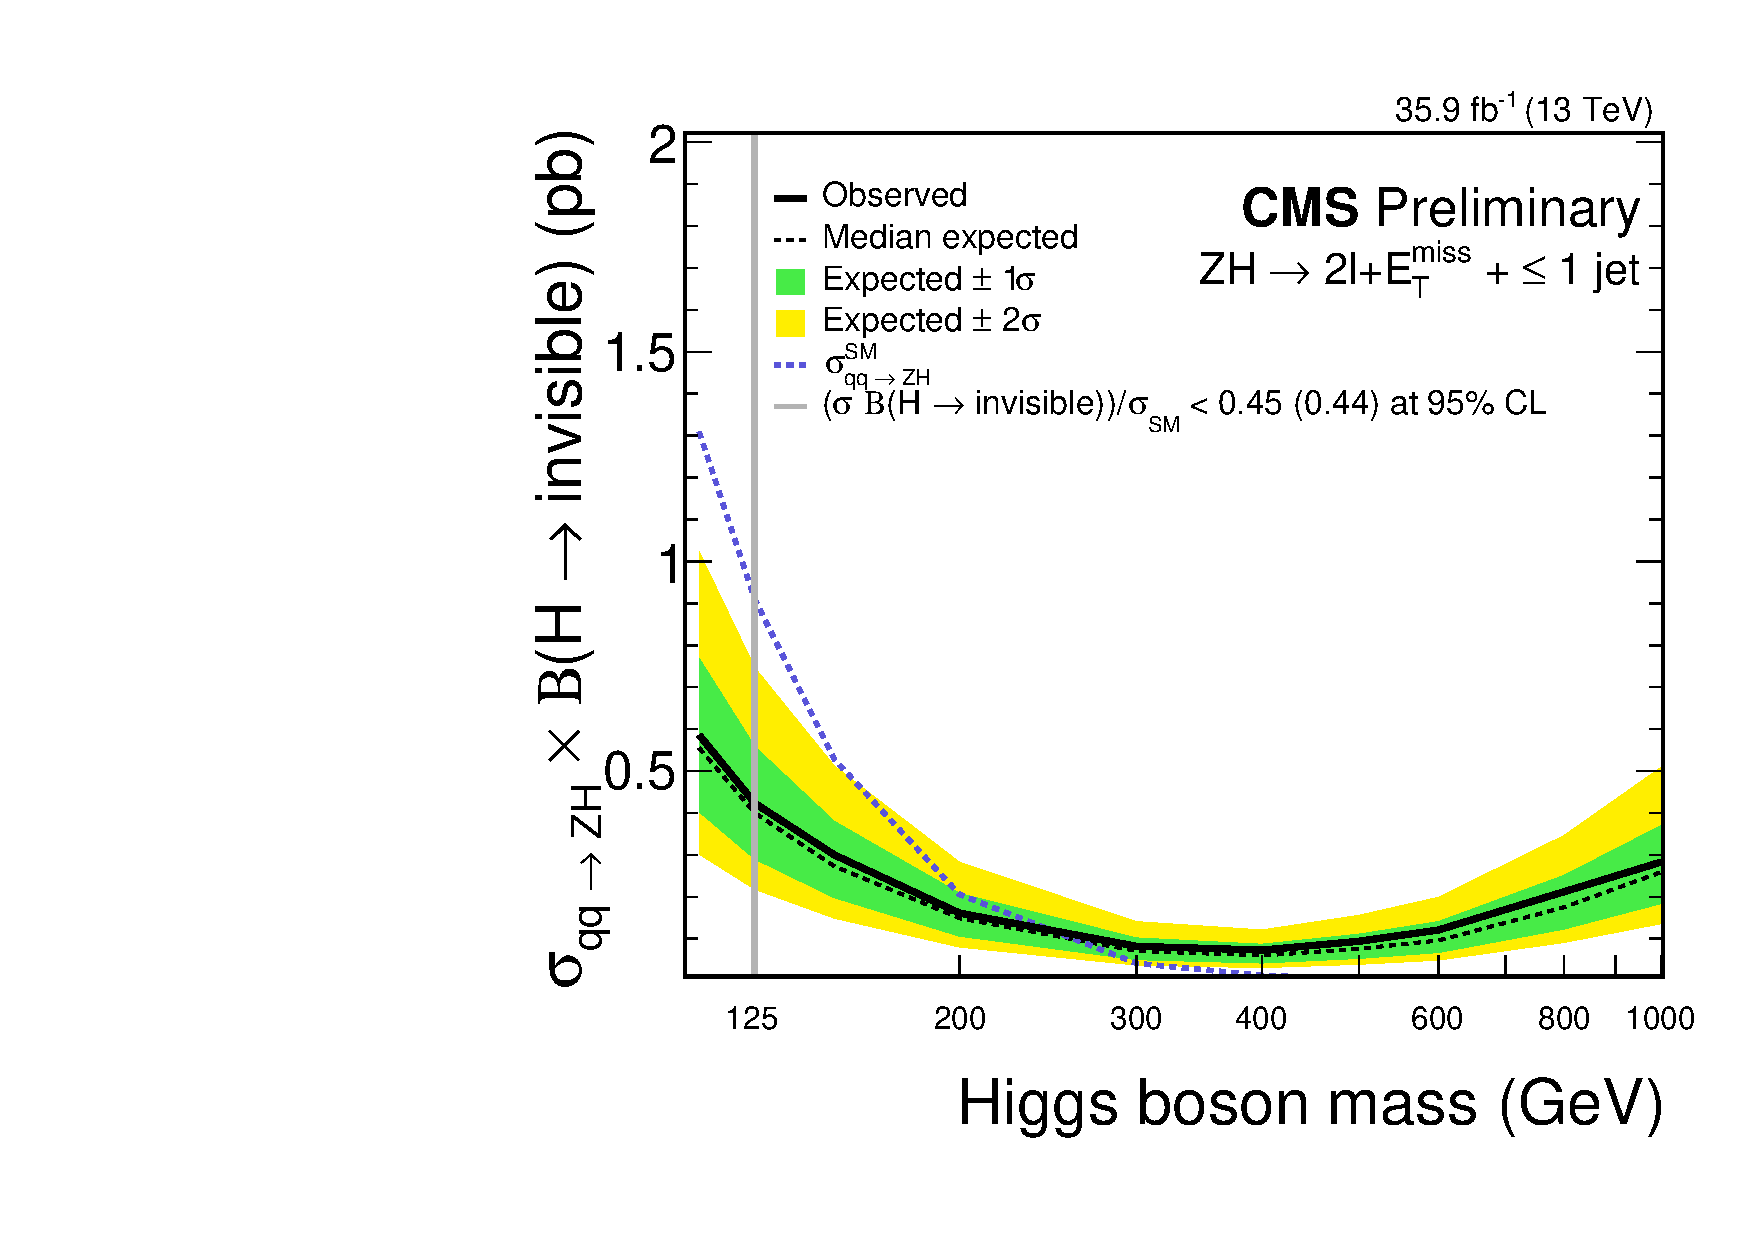
\includegraphics[width=0.55\textwidth]{figures/ana_hzinv_met_nj_from110to1000_logx1_logy0.pdf}}
%\end{figure}

 \begin{figure}[hbtp]
   \begin{center}
 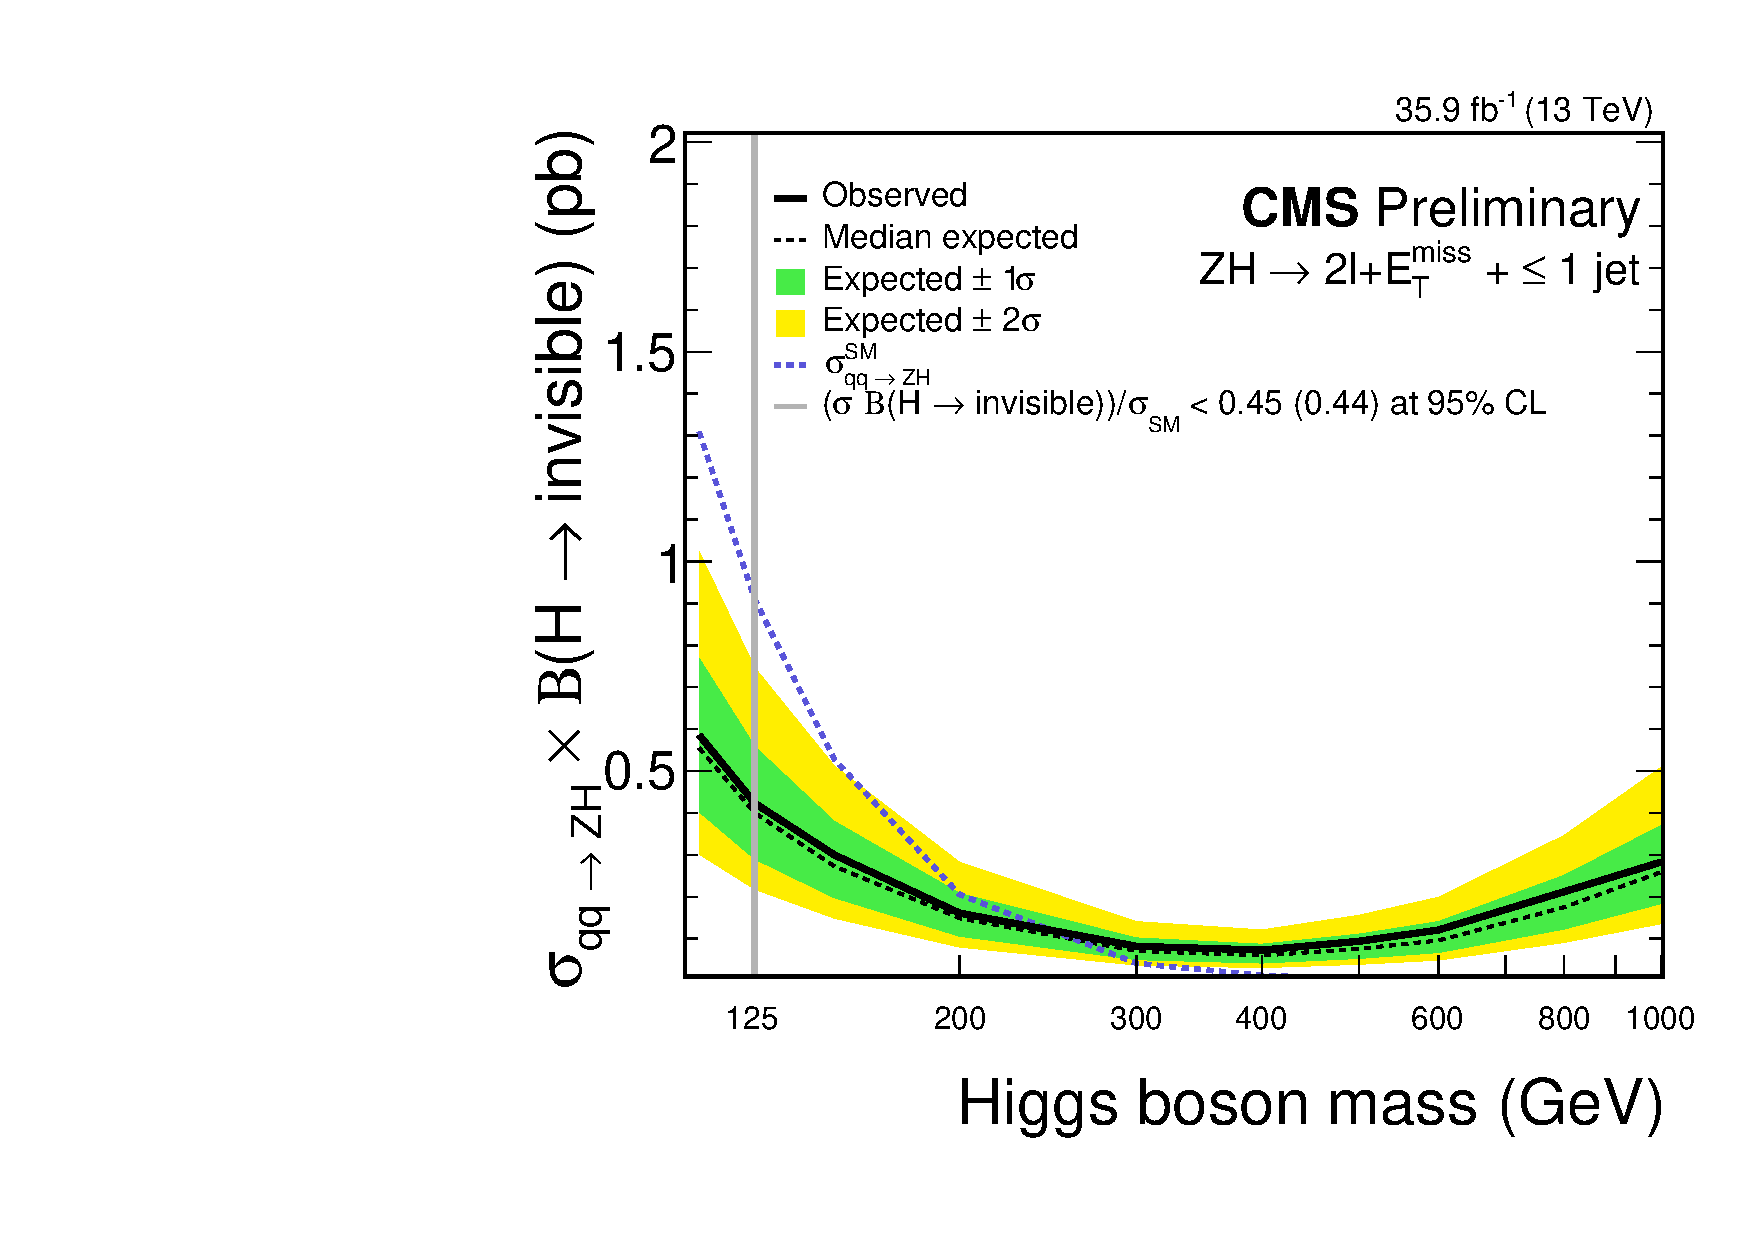
\includegraphics[width=0.65\textwidth]{figures/ana_hzinv_met_nj_from110to1000_logx1_logy0.pdf}
     \caption{Expected and observed 95\% CL upper
        limits on the production cross section times branching ratio, 
 $\sigma_{\Z\Hi(\to \rm invisible)} \times \mathrm{BR}(\Hi \to {\rm invisible})$ as a function 
        of the Higgs boson mass.}
     \label{fig:xsLim}
   \end{center}
 \end{figure}

 \begin{figure}[hbtp]
   \begin{center}
     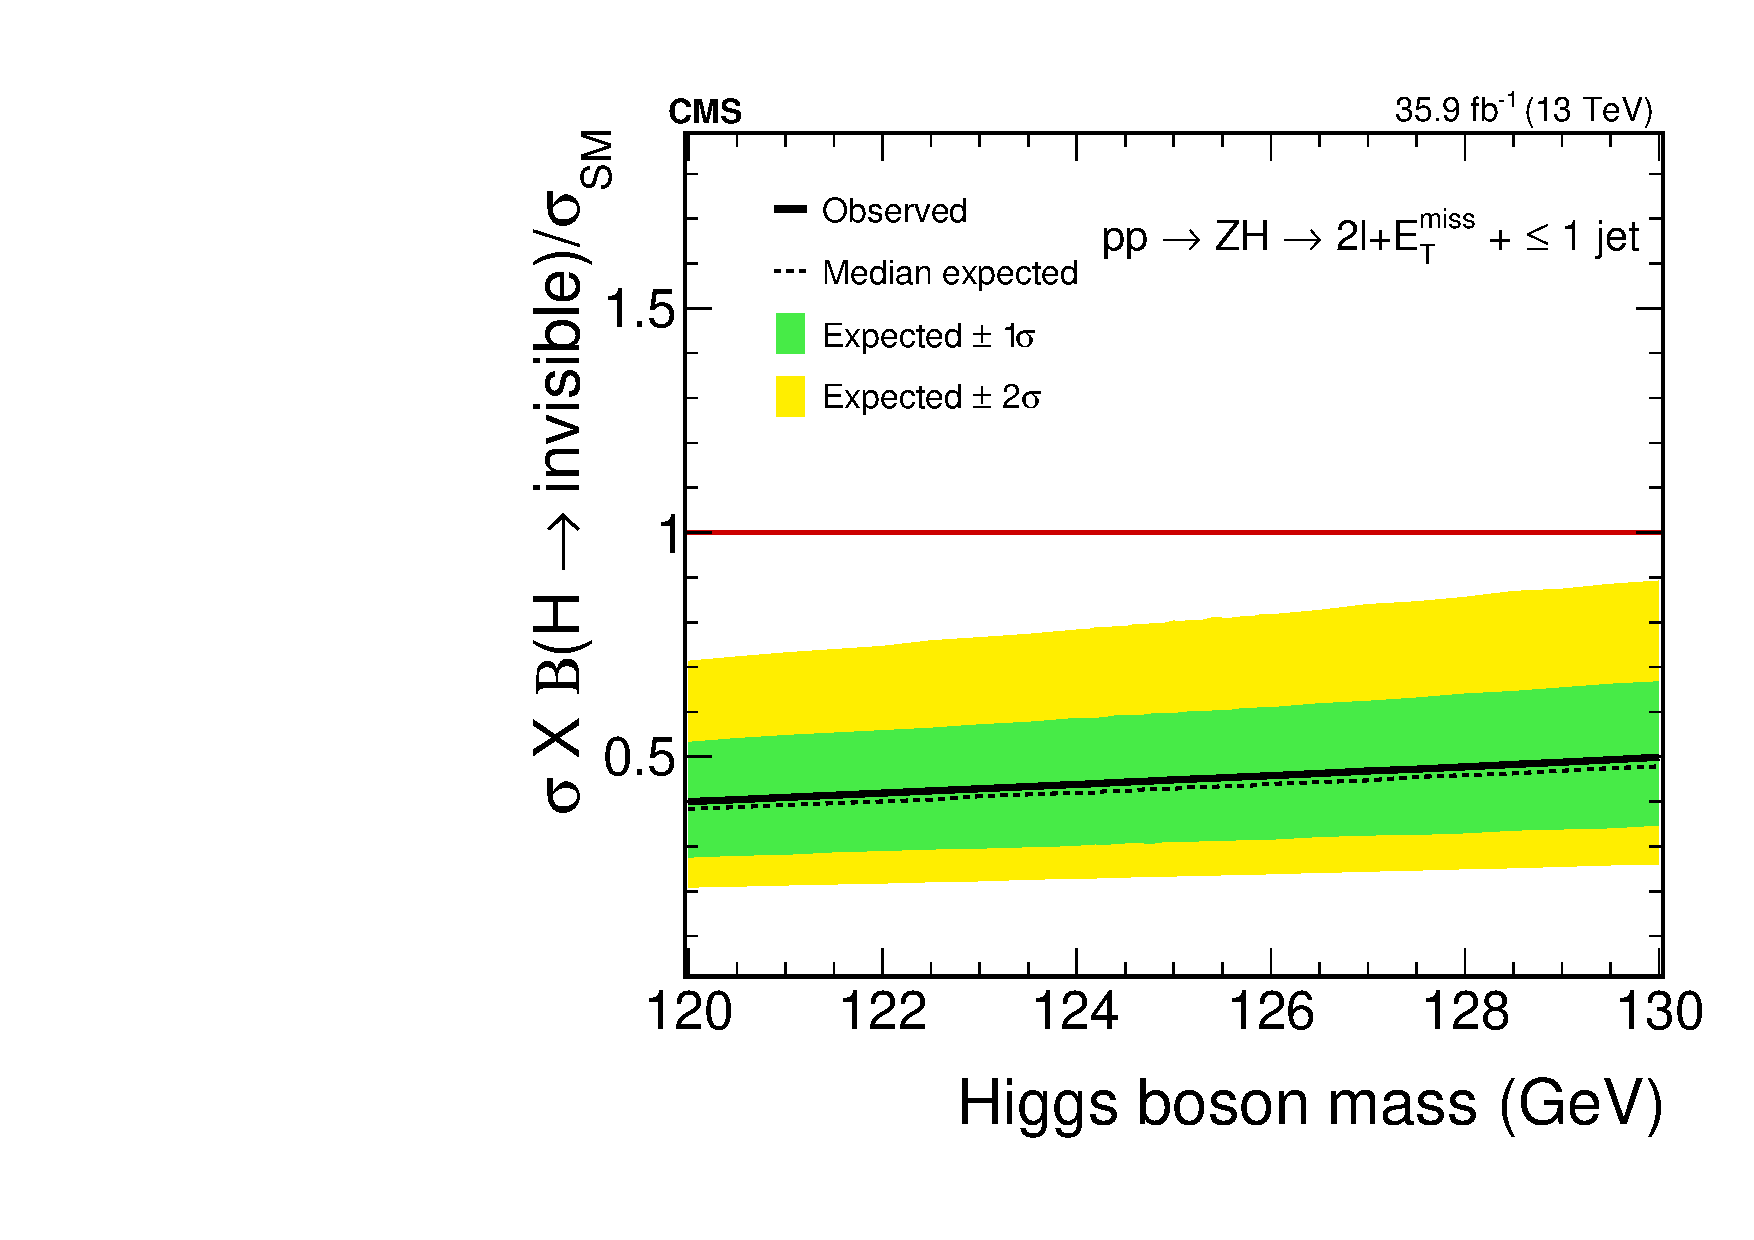
\includegraphics[width=0.65\textwidth]{figures/ana_hzinv_met_nj_massscan_from120to130_logx0_logy0.pdf}
     \caption{
       Expected and observed 95\% CL upper limits on the signal strength, 
       $\sigma_{\Z\Hi(\to \rm invisible)} \times \mathrm{BR}(\Hi \to {\rm invisible})/\sigma_{SM}$ as a function of the Higgs boson mass.
       $\sigma_{SM}$ includes both quark- and gluon-initiated processes.
     }
     \label{fig:xsLim_qqgg}
   \end{center}
 \end{figure}

 \begin{figure}[hbtp]
   \begin{center}
     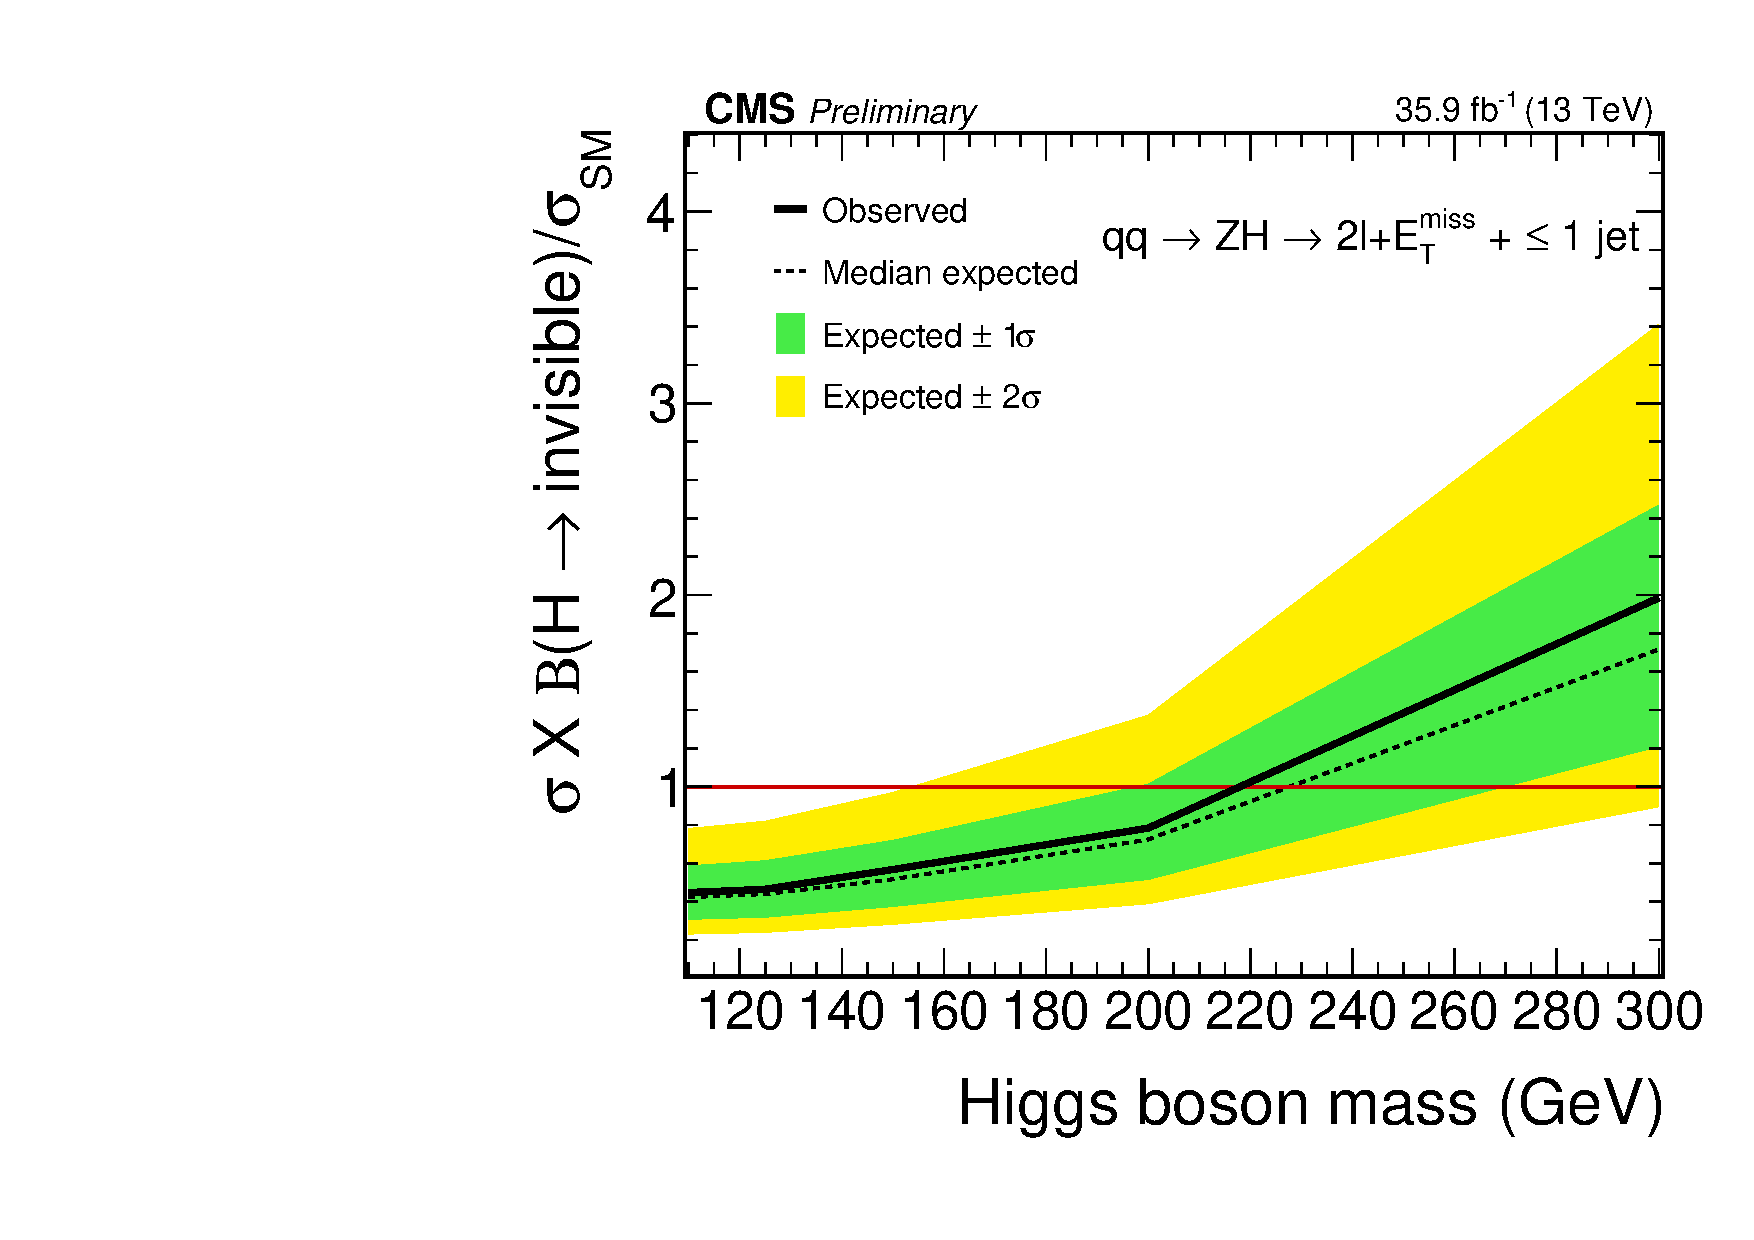
\includegraphics[width=0.65\textwidth]{figures/ana_hzinv_met_nj_ratios_from110to300_logx0_logy0.pdf}
     \caption{
       Expected and observed 95\% CL upper limits on the signal strength, 
       $\sigma_{\Z\Hi(\to \rm invisible)} \times \mathrm{BR}(\Hi \to {\rm invisible})/\sigma_{SM}$ as a function of the Higgs boson mass,
       including only quark-initiated processes.
     }
     \label{fig:xsLim_qq}
   \end{center}
 \end{figure}

\clearpage
\subsection{Simplified Model dark matter interpretation} 

To compute limits on specific DM models, a shape-based analysis is
employed, based on the \ETm distributions in
Fig.~\ref{fig:distributions1}. 
In this case, the test statistics is a binned likelihood. 
Figure~\ref{fig:DM13TeV_MV_MX_gq-0p25} shows the 95\%~CL expected limits for vector and axial-vector mediated scenarios with couplings $g_\chi=1$, $g_q=0.25$.
The plane of mediator and dark matter masses is interpolated between the fully simulated points, which are tabulated in Table~\ref{tab:vector_limits}.
More details on this interpolation procedure may be found in Appendix~\ref{app:interpolation}.
%The same interpolation procedure as in~\cite{exo16010} is followed.

The limits are compared to the results from direct-detection experiments in Fig.~\ref{fig:DDlimits}.
Figure~\ref{fig:DM13TeV_MS_MX_gq-1} shows the 95\%~CL expected limits as a function of $m_{\phi}$ for fixed $m_{\chi}=1\GeV$ with
couplings $g_\chi=1$, $g_q=1$ for scalar and pseudoscalar-vector mediated scenarios.
The expected and observed cross section limits for the different DM signal hypotheses are shown in
Tables~\ref{tab:vector_limits}, \ref{tab:axial_limits}, \ref{tab:pseudoscalar_limits}, \ref{tab:scalar_limits}.

\begin{figure}[hbtp]
  \centering
   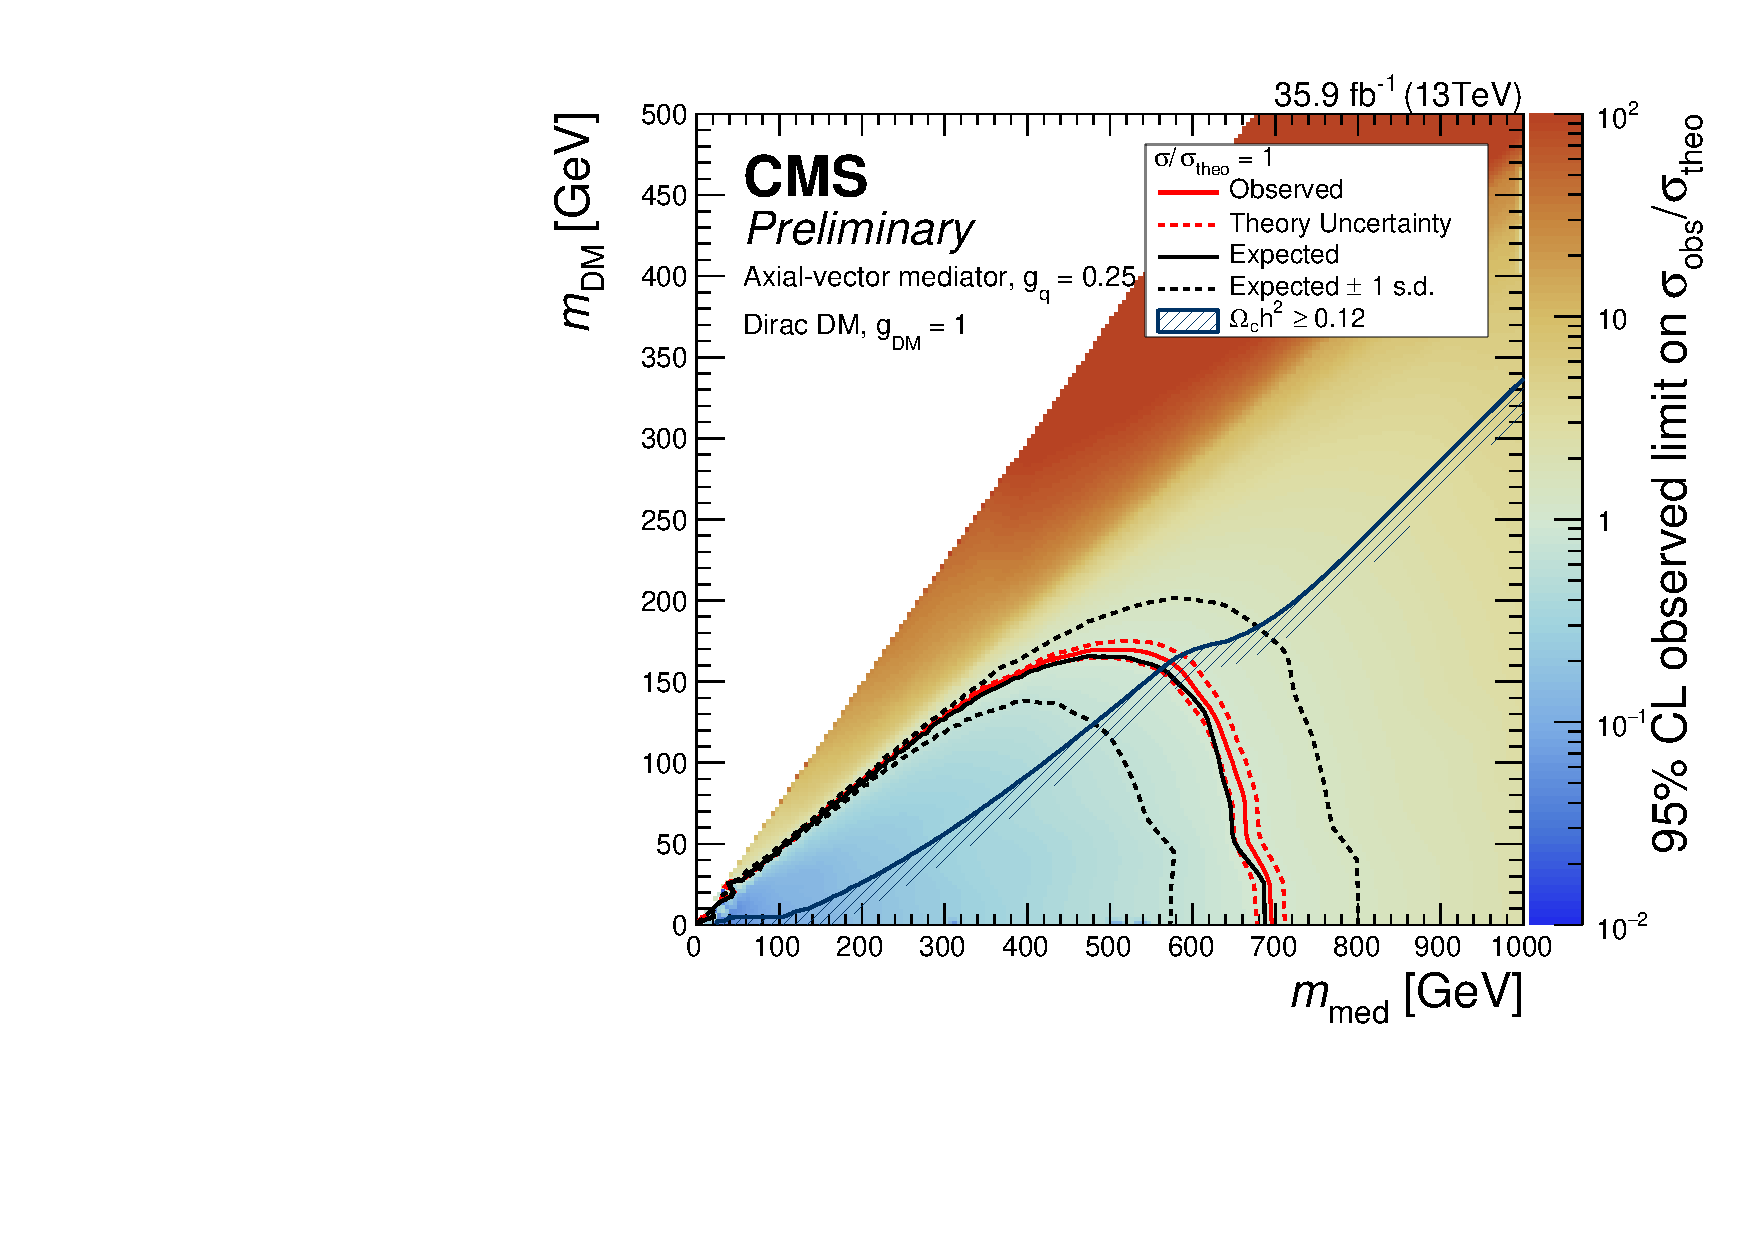
\includegraphics[width=0.48\textwidth]{figures/limit_axial_cl95.pdf}
   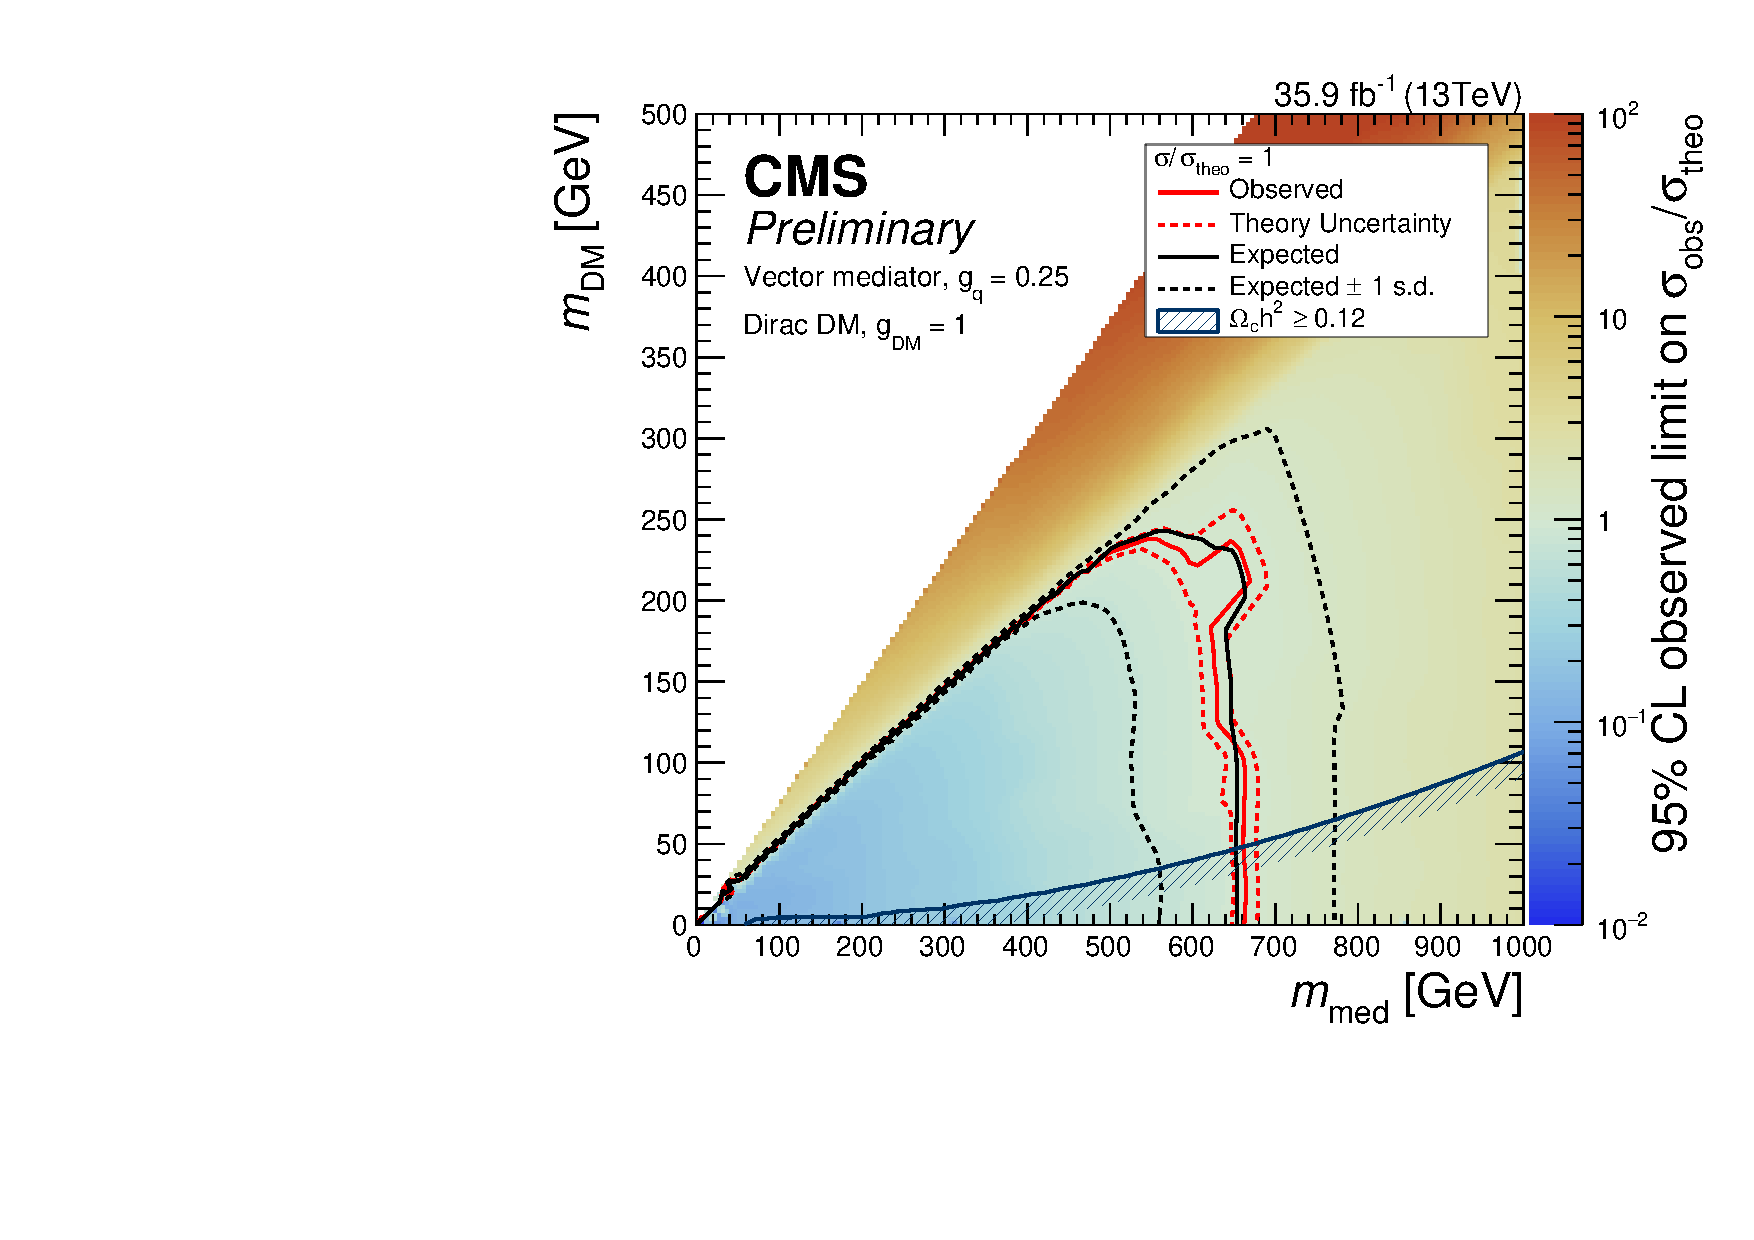
\includegraphics[width=0.48\textwidth]{figures/limit_vector_cl95.pdf}
  \caption{
    The 95\%~\CL expected and observed limits on signal strength $\sigma^{obs}/\sigma^{th}$
    for the axial (left) and vector (right) mediated DM scenario with $g_{q}=0.25$.
    % The 95\%~\CL observed limits on signal strength $\sigma^{obs}/\sigma^{th}$
    % in both vector (left) and axial-vector (right) coupling
    % scenario, for coupling $g_{q}=0.25$. The expected exclusion curves for unity signal
    % strength are shown as a reference.
  } 
  \label{fig:DM13TeV_MV_MX_gq-0p25}
\end{figure}

\begin{figure}[hbtp]
  \centering
   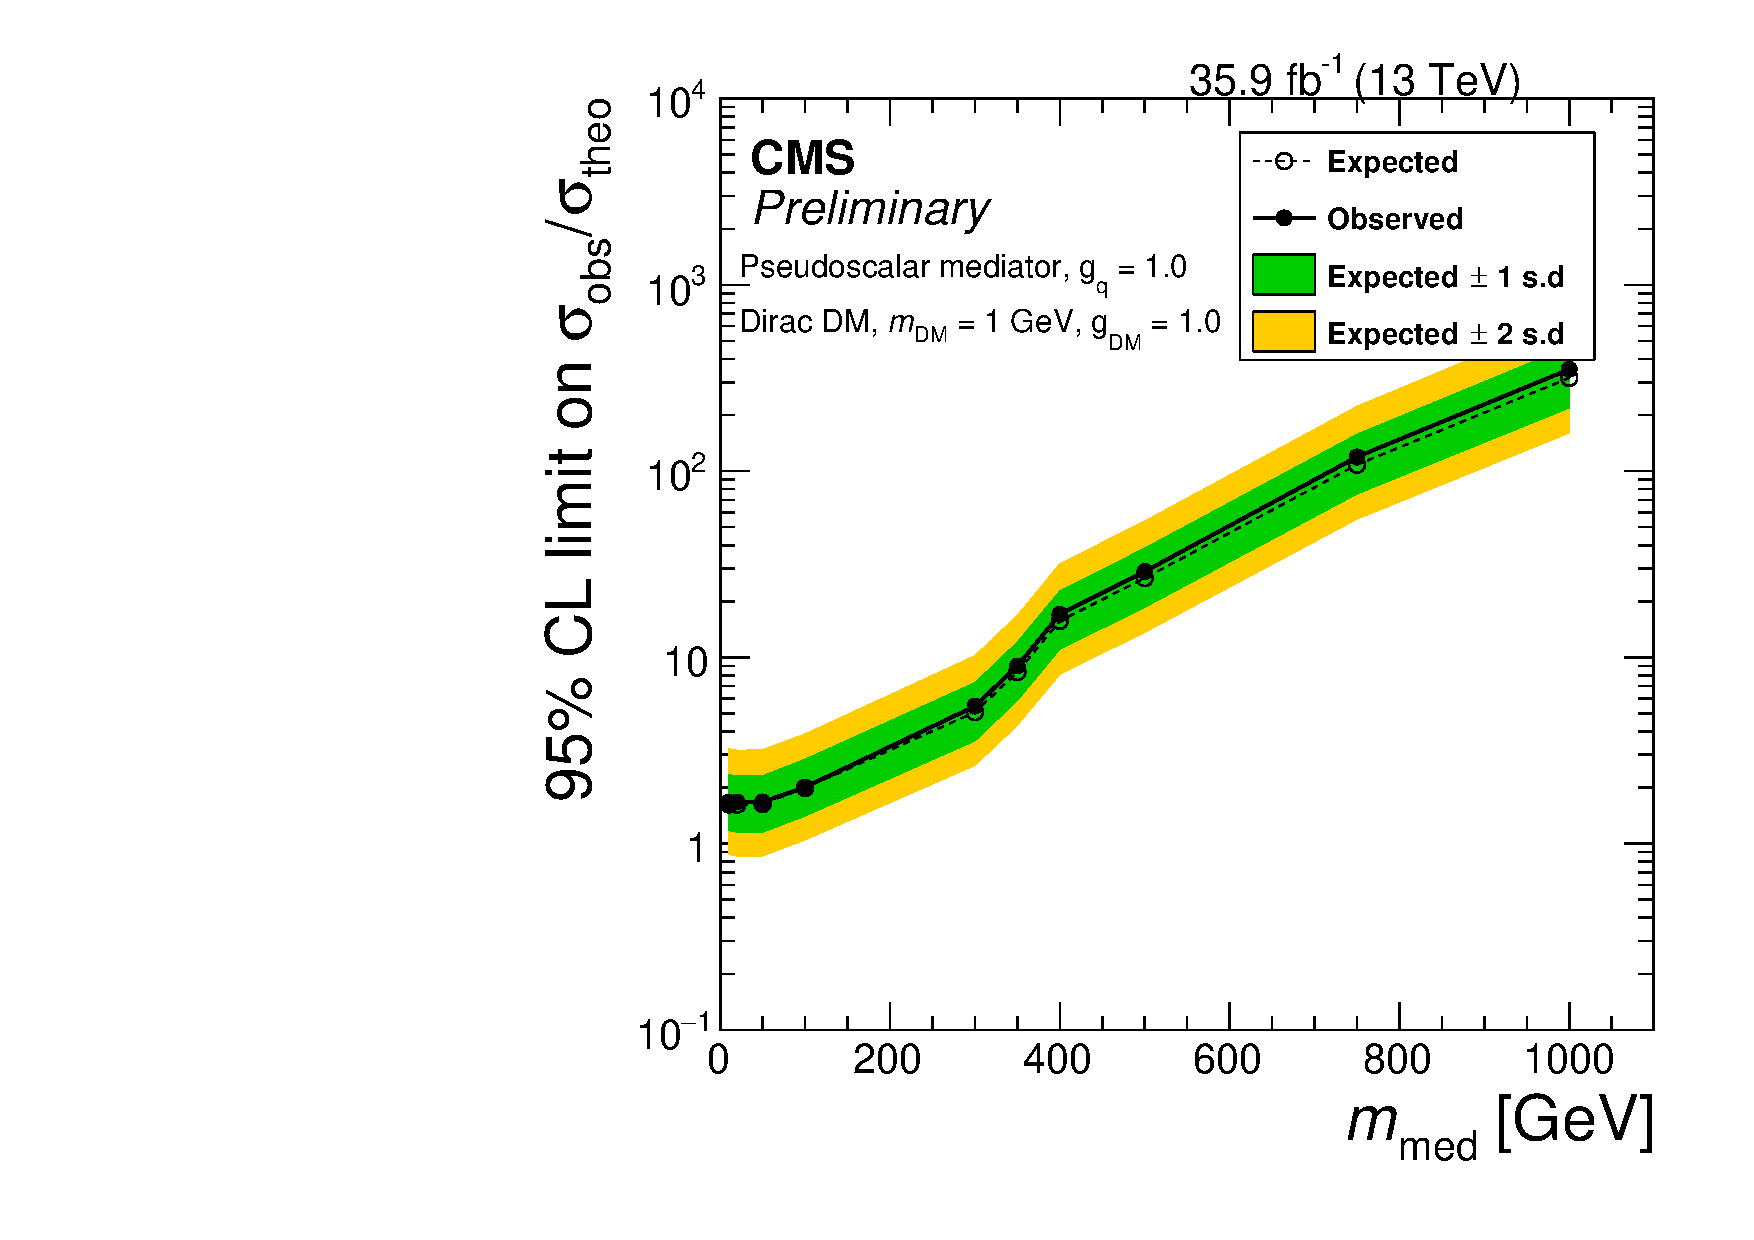
\includegraphics[width=0.48\textwidth]{figures/mu_13TeV_NLOP_Mchi_1.pdf}
   \includegraphics[width=0.48\textwidth]{figures/mu_13TeV_NLOS_Mchi_1.pdf}
  \caption{
    The 95\%~\CL expected and observed limits on signal strength $\sigma^{obs}/\sigma^{th}$
    for the pseudoscalar (left) and scalar (right) mediated DM scenario with $g_{\rm q}=1$.
  } 
  \label{fig:DM13TeV_MS_MX_gq-1}
\end{figure}

\begin{figure}[hbtp]
  \centering
  \includegraphics[width=0.49\textwidth]{figures/Zwimps_13TeV_DM_NucleonXS_SI.pdf}
  \includegraphics[width=0.49\textwidth]{figures/Zwimps_13TeV_DM_NucleonXS_SD.pdf}
  \caption{Observed 90\% CL limits on the DM-nucleon scattering cross sections
          in both spin-independent (left) and spin-dependent (right) cases,
          assuming a mediator-quark coupling constant $g_{\rm q} = 0.25$ and mediator-DM coupling constant $g_{\chi} = 1$. 
          Limits from the LUX~\cite{Akerib:2015rjg}, \mbox{CDMSLite}~\cite{Agnese:2015nto}, PandaX-II~\cite{Tan:2016zwf}, and CRESST-II~\cite{Angloher:2015ewa} experiments are shown for the
          spin-independent case. Limits from the Super-Kamiokande~\cite{Choi:2015ara}, PICO-60~\cite{Amole:2017dex}, and
          IceCube~\cite{Aartsen:2016zhm,Aartsen:2016exj} experiments are shown for the spin-dependent case.
        } 
  \label{fig:DDlimits}
\end{figure}

\begin{table}[hbtp]
  \caption{Expected cross-section limits for a Vector mediator with $\usedLumi$ and couplings $g_\chi=1$, $g_q=0.25$.
  $\mu_{exp}$ corresponds to the expected cross-section limits divided by the theoretical cross section. Limits are with respect to the NLO {\textsc DmSimp} model~\cite{Neubert:2015fka,Backovic:2015soa}}
  \label{tab:vector_limits}
  \begin{center}
{\footnotesize
  \begin{tabular}{rrrrrr}
\hline 
Short title               & $\mu_{exp}$  & $\delta^{+}\mu_{exp}$ & $\delta^{-}\mu_{exp}$ & $\mu_{obs}$  & $\sigma \cdot BR [pb]$ \\
\hline
DM(100)MnloDMV(300)       & 0.29         & 0.4          & 0.21         & 0.33         & 0.0885          \\
DM(10)MnloDMV(10)         & 1.6          & 2.3          & 1.2          & 1.8          & 0.0524          \\
DM(10)MnloDMV(100)        & 0.12         & 0.16         & 0.087        & 0.12         & 0.515           \\
DM(10)MnloDMV(50)         & 0.12         & 0.16         & 0.085        & 0.12         & 0.823           \\
DM(150)MnloDMV(200)       & 10           & 15           & 7.6          & 12           & 0.00184         \\
DM(150)MnloDMV(500)       & 0.72         & 1            & 0.53         & 0.92         & 0.0278          \\
DM(1)MnloDMV(10)          & 1.6          & 2.2          & 1.2          & 1.7          & 0.0545          \\
DM(1)MnloDMV(100)         & 0.14         & 0.19         & 0.1          & 0.15         & 0.516           \\
DM(1)MnloDMV(1000)        & 2.2          & 3.3          & 1.5          & 2.8          & 0.00402         \\
DM(1)MnloDMV(200)         & 0.17         & 0.25         & 0.13         & 0.21         & 0.199           \\
DM(1)MnloDMV(2000)        & 22           & 34           & 15           & 32           & 0.000252        \\
DM(1)MnloDMV(300)         & 0.28         & 0.39         & 0.2          & 0.3          & 0.0949          \\
DM(1)MnloDMV(50)          & 0.12         & 0.17         & 0.085        & 0.13         & 0.841           \\
DM(1)MnloDMV(500)         & 0.57         & 0.82         & 0.41         & 0.7          & 0.029           \\
DM(1)MnloDMV(750)         & 1.2          & 1.8          & 0.86         & 1.5          & 0.00978         \\
DM(300)MnloDMV(750)       & 1.4          & 2            & 1            & 1.9          & 0.00811         \\
DM(40)MnloDMV(100)        & 0.15         & 0.21         & 0.11         & 0.17         & 0.445           \\
DM(490)MnloDMV(1000)      & 5.7          & 8.5          & 3.9          & 8            & 0.00153         \\
DM(500)MnloDMV(500)       & 2e+02        & 3e+02        & 1.4e+02      & 2.7e+02      & 3.63e-05        \\
DM(50)MnloDMV(200)        & 0.2          & 0.28         & 0.15         & 0.22         & 0.194           \\
DM(50)MnloDMV(500)        & 0.59         & 0.83         & 0.42         & 0.68         & 0.0291          \\
DM(75)MnloDMV(500)        & 0.65         & 0.91         & 0.47         & 0.8          & 0.0286          \\
DM(990)MnloDMV(2000)      & 88           & 1.3e+02      & 60           & 1.2e+02      & 7.12e-05        \\
\hline 
  \end{tabular}
}
  \end{center}
\end{table}

\begin{table}[hbtp]
  \caption{Expected cross-section limits for an Axial Vector mediator with $\usedLumi$ and couplings $g_\chi=1$, $g_q=0.25$.
  $\mu_{exp}$ corresponds to the expected cross-section limits divided by the theoretical cross section. Limits are with respect to the NLO {\textsc DmSimp} model.}
  \label{tab:axial_limits}
  \begin{center}
{\footnotesize
  \begin{tabular}{rrrrrr}
\hline 
Short title               & $\mu_{exp}$  & $\delta^{+}\mu_{exp}$ & $\delta^{-}\mu_{exp}$ & $\mu_{obs}$  & $\sigma \cdot BR [pb]$ \\
\hline
DM(100)MnloDMA(300)       & 0.4          & 0.57         & 0.28         & 0.47         & 0.0594          \\
DM(100)MnloDMA(750)       & 1.3          & 1.9          & 0.96         & 1.6          & 0.00925         \\
DM(10)MnloDMA(10)         & 1.6          & 2.2          & 1.1          & 1.9          & 0.0418          \\
DM(10)MnloDMA(100)        & 0.12         & 0.16         & 0.084        & 0.13         & 0.602           \\
DM(10)MnloDMA(50)         & 0.054        & 0.074        & 0.039        & 0.051        & 1.88            \\
DM(140)MnloDMA(300)       & 2.2          & 3.2          & 1.6          & 2.5          & 0.0108          \\
DM(150)MnloDMA(1000)      & 2.6          & 3.7          & 1.8          & 3.4          & 0.00376         \\
DM(150)MnloDMA(200)       & 25           & 35           & 18           & 29           & 0.000693        \\
DM(150)MnloDMA(500)       & 0.89         & 1.3          & 0.65         & 1.1          & 0.0204          \\
DM(1)MnloDMA(10)          & 1.3          & 1.9          & 0.95         & 1.7          & 0.0532          \\
DM(1)MnloDMA(100)         & 0.1          & 0.14         & 0.074        & 0.12         & 0.618           \\
DM(1)MnloDMA(1000)        & 2.2          & 3.2          & 1.5          & 2.8          & 0.00407         \\
DM(1)MnloDMA(200)         & 0.18         & 0.25         & 0.13         & 0.2          & 0.209           \\
DM(1)MnloDMA(2000)        & 22           & 33           & 15           & 29           & 0.000252        \\
DM(1)MnloDMA(300)         & 0.26         & 0.36         & 0.18         & 0.3          & 0.0964          \\
DM(1)MnloDMA(50)          & 0.057        & 0.079        & 0.042        & 0.06         & 1.9             \\
DM(1)MnloDMA(500)         & 0.52         & 0.74         & 0.36         & 0.62         & 0.0307          \\
DM(1)MnloDMA(750)         & 1.1          & 1.6          & 0.76         & 1.4          & 0.01            \\
DM(200)MnloDMA(750)       & 1.7          & 2.4          & 1.2          & 2.2          & 0.00741         \\
DM(300)MnloDMA(750)       & 3.5          & 5.1          & 2.5          & 4.2          & 0.00345         \\
DM(40)MnloDMA(100)        & 0.24         & 0.33         & 0.17         & 0.29         & 0.256           \\
DM(490)MnloDMA(1000)      & 68           & 1e+02        & 47           & 91           & 0.000136        \\
DM(500)MnloDMA(2000)      & 33           & 49           & 22           & 45           & 0.000179        \\
DM(500)MnloDMA(500)       & 6.3e+02      & 9.4e+02      & 4.3e+02      & 8.6e+02      & 1.1e-05         \\
DM(50)MnloDMA(200)        & 0.23         & 0.33         & 0.17         & 0.25         & 0.164           \\
DM(50)MnloDMA(300)        & 0.32         & 0.45         & 0.23         & 0.37         & 0.0896          \\
DM(50)MnloDMA(50)         & 5.3          & 7.4          & 3.8          & 5.7          & 0.00591         \\
DM(50)MnloDMA(500)        & 0.55         & 0.78         & 0.39         & 0.63         & 0.0294          \\
DM(75)MnloDMA(1000)       & 2.2          & 3.3          & 1.6          & 3            & 0.00398         \\
DM(75)MnloDMA(500)        & 0.63         & 0.89         & 0.45         & 0.75         & 0.0279          \\
DM(990)MnloDMA(2000)      & 1.3e+03      & 2e+03        & 8.9e+02      & 1.9e+03      & 4.64e-06        \\
\hline
\end{tabular}
}
  \end{center}
\end{table}

\begin{table}[hbtp]
  \caption{
    Expected and observed signal strength limits for NLO Simplified Model Pseudoscalar-mediated Dark Matter samples with $\usedLumi$.
    $\mu_{obs},$ and $\mu_{exp}$ correspond to the observed and expected cross-section limits divided by the theoretical cross section.
    The cross section times branching ratio is also listed for reference.
    The mapping from short title to dataset is as follows:
    {\footnotesize DM($m_\chi$)MnloDMP($m_\mathrm{med}$) $\rightarrow$ DarkMatter\_MonoZToLL\_NLO\_Pseudo\_Mx-\$mchi\_Mv-\$mmed\_gDM1\_gQ1\_TuneCUETP8M1\_13TeV-madgraph }
  }
  \label{tab:pseudoscalar_limits}
  \begin{center}
{\footnotesize
  \begin{tabular}{rrrrrr}
\hline 
Short title               & $\mu_{exp}$  & $\delta^{+}\mu_{exp}$ & $\delta^{-}\mu_{exp}$ & $\mu_{obs}$  & $\sigma \cdot BR [pb]$ \\
\hline
DM(100)MnloDMP(300)       & 6.3          & 8.9          & 4.6          & 8.4          & 0.00255         \\
DM(100)MnloDMP(350)       & 11           & 15           & 7.7          & 14           & 0.00138         \\
DM(100)MnloDMP(500)       & 35           & 50           & 25           & 48           & 0.000288        \\
DM(100)MnloDMP(750)       & 1.2e+02      & 1.7e+02      & 87           & 1.7e+02      & 6.78e-05        \\
DM(10)MnloDMP(10)         & 33           & 46           & 24           & 41           & 0.00056         \\
DM(10)MnloDMP(100)        & 2.3          & 3.1          & 1.7          & 2.7          & 0.00871         \\
DM(10)MnloDMP(50)         & 2            & 2.8          & 1.5          & 2.5          & 0.00972         \\
DM(1)MnloDMP(10)          & 1.9          & 2.7          & 1.4          & 2.3          & 0.0102          \\
DM(1)MnloDMP(100)         & 2.4          & 3.3          & 1.7          & 2.8          & 0.00879         \\
DM(1)MnloDMP(1000)        & 3.4e+02      & 4.9e+02      & 2.4e+02      & 4.9e+02      & 2.16e-05        \\
DM(1)MnloDMP(20)          & 1.9          & 2.7          & 1.4          & 2.3          & 0.0101          \\
DM(1)MnloDMP(300)         & 6            & 8.4          & 4.3          & 7.9          & 0.00254         \\
DM(1)MnloDMP(350)         & 9.8          & 14           & 7            & 13           & 0.00148         \\
DM(1)MnloDMP(400)         & 18           & 26           & 13           & 25           & 0.000683        \\
DM(1)MnloDMP(50)          & 1.9          & 2.7          & 1.4          & 2.3          & 0.00972         \\
DM(1)MnloDMP(500)         & 31           & 44           & 22           & 42           & 0.000323        \\
DM(1)MnloDMP(750)         & 1.2e+02      & 1.8e+02      & 89           & 1.7e+02      & 7.02e-05        \\
DM(200)MnloDMP(500)       & 47           & 66           & 34           & 64           & 0.000213        \\
DM(350)MnloDMP(1000)      & 4.7e+02      & 6.9e+02      & 3.3e+02      & 6.8e+02      & 1.57e-05        \\
DM(350)MnloDMP(750)       & 2.9e+02      & 4.2e+02      & 2.1e+02      & 4.1e+02      & 2.99e-05        \\
DM(40)MnloDMP(100)        & 2.3          & 3.1          & 1.6          & 2.8          & 0.00876         \\
DM(50)MnloDMP(10)         & 1e+02        & 1.5e+02      & 75           & 1.3e+02      & 0.000151        \\
DM(50)MnloDMP(200)        & 4.3          & 6            & 3.1          & 5.5          & 0.00418         \\
DM(50)MnloDMP(300)        & 6            & 8.4          & 4.3          & 7.9          & 0.00248         \\
DM(50)MnloDMP(350)        & 10           & 14           & 7.2          & 13           & 0.00148         \\
DM(50)MnloDMP(400)        & 17           & 24           & 12           & 23           & 0.00069         \\
DM(50)MnloDMP(50)         & 92           & 1.3e+02      & 67           & 1.2e+02      & 0.000178        \\
DM(50)MnloDMP(500)        & 32           & 45           & 23           & 44           & 0.000304        \\
\hline 
  \end{tabular}
}
  \end{center}
\end{table}

\begin{table}[hbtp]
  \caption{
    Expected and observed signal strength limits for NLO Simplified Model Scalar-mediated Dark Matter samples with $\usedLumi$.
    $\mu_{obs},$ and $\mu_{exp}$ correspond to the observed and expected cross-section limits divided by the theoretical cross section.
    The cross section times branching ratio is also listed for reference.
    The mapping from short title to dataset is as follows:
    {\footnotesize DM(\$mchi)MnloDMS(\$mmed) $\rightarrow$ DarkMatter\_MonoZToLL\_NLO\_Scalar\_Mx-\$mchi\_Mv-\$mmed\_gDM1\_gQ1\_TuneCUETP8M1\_13TeV-madgraph }
  }
  \label{tab:scalar_limits}
  \begin{center}
{\footnotesize
  \begin{tabular}{rrrrrr}
\hline 
Short title               & $\mu_{exp}$  & $\delta^{+}\mu_{exp}$ & $\delta^{-}\mu_{exp}$ & $\mu_{obs}$  & $\sigma \cdot BR [pb]$ \\
\hline
DM(0)MnloDMS(20)          & 2.3          & 3.2          & 1.7          & 2.7          & 0.00739         \\
DM(100)MnloDMS(300)       & 5.1          & 7.1          & 3.7          & 6.4          & 0.00257         \\
DM(100)MnloDMS(350)       & 6.2          & 8.7          & 4.5          & 8.2          & 0.00192         \\
DM(100)MnloDMS(400)       & 10           & 15           & 7.4          & 14           & 0.00105         \\
DM(100)MnloDMS(500)       & 23           & 33           & 17           & 32           & 0.00039         \\
DM(10)MnloDMS(10)         & 45           & 63           & 33           & 56           & 0.000346        \\
DM(10)MnloDMS(100)        & 2.6          & 3.6          & 1.9          & 3.2          & 0.00616         \\
DM(10)MnloDMS(50)         & 2.3          & 3.1          & 1.6          & 2.7          & 0.00722         \\
DM(1)MnloDMS(1000)        & 3.2e+02      & 4.6e+02      & 2.3e+02      & 4.6e+02      & 2.12e-05        \\
DM(1)MnloDMS(20)          & 2.3          & 3.2          & 1.7          & 2.7          & 0.00733         \\
DM(1)MnloDMS(200)         & 3.5          & 4.9          & 2.6          & 4.4          & 0.00433         \\
DM(1)MnloDMS(300)         & 5.2          & 7.3          & 3.8          & 6.7          & 0.00253         \\
DM(1)MnloDMS(350)         & 6.5          & 9.2          & 4.7          & 8.6          & 0.00185         \\
DM(1)MnloDMS(400)         & 10           & 14           & 7.3          & 13           & 0.00112         \\
DM(1)MnloDMS(50)          & 2.3          & 3.2          & 1.7          & 2.8          & 0.00708         \\
DM(1)MnloDMS(500)         & 22           & 32           & 16           & 30           & 0.000421        \\
DM(1)MnloDMS(750)         & 94           & 1.4e+02      & 66           & 1.3e+02      & 7.95e-05        \\
DM(200)MnloDMS(500)       & 48           & 67           & 34           & 65           & 0.000191        \\
DM(350)MnloDMS(1000)      & 6.6e+02      & 9.6e+02      & 4.6e+02      & 9.4e+02      & 9.48e-06        \\
DM(350)MnloDMS(750)       & 8.9e+02      & 1.3e+03      & 6.2e+02      & 1.3e+03      & 7.51e-06        \\
DM(40)MnloDMS(100)        & 2.5          & 3.5          & 1.8          & 3.1          & 0.0065          \\
DM(450)MnloDMS(1000)      & 1.9e+03      & 2.9e+03      & 1.3e+03      & 3e+03        & 2.74e-06        \\
DM(50)MnloDMS(10)         & 1.7e+02      & 2.4e+02      & 1.3e+02      & 2.2e+02      & 8.25e-05        \\
DM(50)MnloDMS(200)        & 3.6          & 5            & 2.6          & 4.5          & 0.00426         \\
DM(50)MnloDMS(300)        & 4.9          & 6.9          & 3.6          & 6.4          & 0.00257         \\
DM(50)MnloDMS(350)        & 6.2          & 8.7          & 4.5          & 8.1          & 0.00189         \\
DM(50)MnloDMS(400)        & 9.5          & 13           & 6.8          & 13           & 0.00113         \\
DM(50)MnloDMS(50)         & 1.5e+02      & 2.1e+02      & 1.1e+02      & 1.9e+02      & 9.31e-05        \\
\hline 
  \end{tabular}
}
  \end{center}
\end{table}


\clearpage
\subsection{Unparticle interpretation}
In the unparticle scenario, a shape analysis of the $\met$ spectrum is performed.
Upper limits are set on the Wilson coefficient $\lambda / \LU^{\dU-1}$ of the unparticle-quark coupling operator.
Additionally, lower limits are set on the cutoff scale \LU, assuming a fixed value of the coupling $\lambda=1$.

The limits both variables are calculated at 95\% CL and shown in Fig.~\ref{fig:unparticleLimits} as a function of the scaling dimension $d_{\textsf U}$.
Limits on the production cross-section as a function of \dU are shown in Fig.~\ref{fig:unparticleLimits2}.
The exclusion limits for each parameter point are given in Tab.~\ref{tab:addunpart_limits}.


\begin{figure}[hbtp]
  \centering
   \includegraphics[width=0.46\textwidth]{figures/unparticles/limit_unparticle_alpha.pdf}
   \includegraphics[width=0.46\textwidth]{figures/unparticles/limit_unparticle_lambda_u_noref.pdf}
  \caption{
			Left: The 95\% CL upper limits on the Wilson coefficient $\lambda / \LU^{\dU-1}$ of the unparticle-quark coupling operator.
			Right: The 95\% CL lower limits on unparticle effective cutoff scale \LU for a fixed coupling $\lambda=1$.
			The results from a previous CMS mono-Z search~\cite{Khachatryan:2015bbl} are shown for comparison.
  }
  \label{fig:unparticleLimits}
\end{figure}
\begin{figure}[hbtp]
  \centering
   \includegraphics[width=0.46\textwidth]{figures/unparticles/limit_unparticle_xs.pdf}
  \caption{
			The 95\% CL upper limits on the cross-section for $pp\rightarrow U\Z$ in the unparticle model.
  }
  \label{fig:unparticleLimits2}
\end{figure}












\begin{table}[hbtp]
  \caption{
    Expected and observed signal strength limits for Large Extra Dimension and Unparticle samples with $\usedLumi$.
    $\mu_{obs},$ and $\mu_{exp}$ correspond to the observed and expected cross-section limits divided by the theoretical cross section.
    The cross section times branching ratio is also listed for reference.
    In both ADD and unparticles the given cross-section is the one produced by pythia for the respective sample.
    The Z branching fractions are not included. The truncation in the ADD case is also not included.
    The properly truncated ADD cross-sections are given in Appendix~\ref{app:add_xs}.
  }
  \label{tab:addunpart_limits}
  \begin{center}
{\footnotesize
  \begin{tabular}{rrrrrr}
\hline 
Short title               & $\mu_{exp}$  & $\delta^{+}\mu_{exp}$ & $\delta^{-}\mu_{exp}$ & $\mu_{obs}$  & $\sigma$ [pb]\\
\hline
ADD $M_{D} = 3\TeV$, $n=2$               & 0.11         & 0.17         & 0.074        & 0.15         & 0.0342          \\
ADD $M_{D} = 3\TeV$, $n=3$               & 0.097        & 0.15         & 0.065        & 0.13         & 0.032           \\
ADD $M_{D} = 3\TeV$, $n=4$               & 0.076        & 0.12         & 0.05         & 0.1          & 0.0369          \\
ADD $M_{D} = 3\TeV$, $n=5$               & 0.052        & 0.082        & 0.035        & 0.071        & 0.0472          \\
ADD $M_{D} = 3\TeV$, $n=6$               & 0.037        & 0.057        & 0.024        & 0.05         & 0.0648          \\
ADD $M_{D} = 3\TeV$, $n=7$               & 0.024        & 0.038        & 0.016        & 0.033        & 0.0939          \\
Unparticle, $\dU=1.01$, $\LU=15\TeV$ &   0.033 &    0.013 &    0.009 &    0.031 & 28.2 \\
Unparticle, $\dU=1.02$, $\LU=15\TeV$ &   0.020 &    0.007 &    0.005 &    0.019 & 46.7 \\
Unparticle, $\dU=1.04$, $\LU=15\TeV$ &   0.014 &    0.006 &    0.004 &    0.014 & 64.4 \\
Unparticle, $\dU=1.06$, $\LU=15\TeV$ &   0.013 &    0.005 &    0.004 &    0.012 & 66.7 \\
Unparticle, $\dU=1.09$, $\LU=15\TeV$ &   0.016 &    0.006 &    0.004 &    0.016 & 57.9 \\
Unparticle, $\dU=1.10$, $\LU=15\TeV$ &   0.016 &    0.006 &    0.004 &    0.014 & 53.7 \\
Unparticle, $\dU=1.20$, $\LU=15\TeV$ &   0.041 &    0.016 &    0.011 &    0.038 & 17.9 \\
Unparticle, $\dU=1.30$, $\LU=15\TeV$ &    0.13 &    0.052 &    0.036 &    0.13  &  4.7 \\
Unparticle, $\dU=1.40$, $\LU=15\TeV$ &    0.40 &     0.16 &     0.11 &    0.38  &  1.1 \\
Unparticle, $\dU=1.50$, $\LU=15\TeV$ &     1.4 &     0.56 &     0.40 &    1.30  &  0.29 \\
Unparticle, $\dU=1.60$, $\LU=15\TeV$ &     4.8 &     1.93 &     1.37 &    4.5   &  0.073 \\
Unparticle, $\dU=1.70$, $\LU=15\TeV$ &    14.8 &     6.20 &      4.2 &   14.0   &  0.019 \\
Unparticle, $\dU=1.80$, $\LU=15\TeV$ &    50.7 &    21.23 &     14.8 &   47.6   &  0.0048 \\
Unparticle, $\dU=1.90$, $\LU=15\TeV$ &     167 &     71.1 &     48.1 &  163     &  0.00127 \\
Unparticle, $\dU=2.00$, $\LU=15\TeV$ &     534 &      224 &      155 &  512     &  0.000345 \\
Unparticle, $\dU=2.20$, $\LU=15\TeV$ &  5.2e+3 &   2.3e+3 &   1.5e+3 & 5.0e+3   &  2.71e-5 \\\hline
  \end{tabular}
}
  \end{center}
\end{table}



\clearpage

 \subsection{ADD Interpretation}
In the framework of the ADD model of extra dimensions, limits are calculated depending on the number of extra dimensions $n$ and $M_{D}$.
For each value of $d$, cross-section limits are calculated as a function of $M_{D}$ (fig.~\ref{fig:limits_add_xs}).
By finding the intersection between the theory cross-section line with the observed and expected excluded cross-sections,
and projecting that point onto the $M_{D}$ axis, limits on $M_{D}$ are found as a function of $n$ (fig.~\ref{fig:limits_add_md}).
The used theoretical cross sections are given in appendix~\ref{app:add_xs} and shown graphically in fig.~\ref{fig:xs_add_md}.

The observed (expected) exclusion of $M_{D}$ ranges between $2.1$ and $2.4$ \TeV ($2.3$ and $2.6$ \TeV) for $n$ between 2 and 7.

To illustrate the impact of the truncation procedure, the cross-sections with and without truncation are shown in fig.~\ref{fig:xs_add_md}.
The truncation has a greater impact on scenarios with more extra dimensions. The relative spread between low-$n$ and high-$n$ scenarios is thus greatly reduced by the truncation and the cross-sections converge.

\begin{figure}[hbtp]
  \centering
  \includegraphics[width=0.7\textwidth]{figures/ADD/add_limit_md.pdf}
  \caption{Expected and observed exclusion limits on $M_{D}$ as a function of $n$.
  }
  \label{fig:limits_add_md}
\end{figure}

\begin{figure}[hbtp]
  \centering
    \includegraphics[width=0.48\textwidth]{figures/ADD/add_limit_nd2.pdf}
    \includegraphics[width=0.48\textwidth]{figures/ADD/add_limit_nd3.pdf}

    \includegraphics[width=0.48\textwidth]{figures/ADD/add_limit_nd4.pdf}
    \includegraphics[width=0.48\textwidth]{figures/ADD/add_limit_nd5.pdf}

    \includegraphics[width=0.48\textwidth]{figures/ADD/add_limit_nd6.pdf}
    \includegraphics[width=0.48\textwidth]{figures/ADD/add_limit_nd7.pdf}

  \caption{Cross-section limits in the ADD scenario as a function of $M_{D}$ for different values of $n$.
		   The Red curve shows the theoretical cross-section for given values of $n$.
		   The cross-sections are calculated for the fiducal phase-space of $\pt(\rm Graviton) > 50\GeV$.
			Gray lines show the projection of the intersection between theory and expected (observed) exclusion onto the $M_{D}$ axis.
  }
    \label{fig:limits_add_xs}
\end{figure}

\begin{figure}[hbtp]
  \centering
  \includegraphics[width=0.48\textwidth]{figures/ADD/ADD_xs_v_md_truncated.pdf}
  \includegraphics[width=0.48\textwidth]{figures/ADD/ADD_xs_v_md_untruncated.pdf}
  \caption{Truncated (left) and untruncated (right) cross-sections for the ADD model as a function of $M_{D}$. Each curve represents one value of $n$.
			The effect of the truncation increases with $n$. The truncated values are used for limit-setting. The untruncated graphs are shown only for illustration.
			The cross-sections are calculated for the fiducal phase-space of $\pt(\rm Graviton) > 50\GeV$.
  }
  \label{fig:xs_add_md}
\end{figure}

\clearpage
\subsection{Simplified Likelihood}
The observed event yields and total expected background yields in the signal region are tabulated in Tab.~\ref{tab:binnedCounts_sr}.
The correlation between $\met$ bins in the signal region is shown in Fig.~\ref{fig:correlation}.
This allows re-interpretation of the results in this paper according to the simplified likelihood approach, as described in Ref.~\cite{simplified-likelihood}

To test the validity of the re-interpretation, a closure test was performed using the Higgs invisible signal model.
The median expected 95\% CL signal strength limit for a Higgs invisible signal was 0.45, as compared to 0.43 for the full likelihood model.
A comparison of the likelihood as a function of signal strength $\mu$ is shown in Fig.~\ref{fig:simplified_likelihood_closure}.

\begin{table}[hbtp]
  \caption{
    Expected event yields in each $\met$ bin for the sum of background processes in the signal region.
    The background yields and their corresponding uncertainties are obtained after performing a combined fit
    to data in all control regions, but excluding data in the signal region.
    The observed events in each bin are also included.
  }
  \label{tab:binnedCounts_sr}
  \begin{center}
{\footnotesize
  \begin{tabular}{lcc}
\hline 
$\met$ Bin             & Observed events & Total background prediction \\
\hline
$100 \leq \met < 125$  & 311             & $256\pm32$           \\
$125 \leq \met < 150$  & 155             & $150\pm12$           \\
$150 \leq \met < 175$  & 87              & $86.9\pm8.4$         \\
$175 \leq \met < 200$  & 50              & $52.7\pm5.3$         \\
$200 \leq \met < 250$  & 56              & $50.2\pm4.9$         \\
$250 \leq \met < 300$  & 15              & $19.4\pm2.2$         \\
$300 \leq \met < 350$  & 11              & $9.4\pm1.2$          \\
$350 \leq \met < 400$  & 6               & $4.58\pm0.66$        \\
$400 \leq \met < 500$  & 6               & $3.31\pm0.54$        \\
$500 \leq \met$        & 1               & $1.57\pm0.33$        \\
\hline 
  \end{tabular}
}
  \end{center}
\end{table}

\begin{figure}[hbtp]
  \centering
  \includegraphics[width=0.6\textwidth]{figures/correlation.pdf}
  \caption{
    Correlations between the uncertainties in the estimated background yields in the signal region $\met$ bins.
    The correlations are obtained after performing a combined fit to data in all control regions, but excluding data in the signal region.
  }
  \label{fig:correlation}
\end{figure}

\begin{figure}[hbtp]
  \centering
  \includegraphics[width=0.6\textwidth]{figures/smHiggs_likelihoodScan_comp.pdf}
  \caption{
    Comparison of likelihood scans for the full likelihood model and the simplified likelihood, for the Higgs invisible signal.
    Good agreement is shown, confirming that the simplified likelihood approximation is valid in this analysis.
  }
  \label{fig:simplified_likelihood_closure}
\end{figure}
